\documentclass%
%[handout]
{beamer}
\newcommand{\currentLecture}{12}
\newcommand{\semester}{Summer 2015}
% % % % % % % %
% % % % % % % %
% % % % % % % %
%IMPORTANT
%compiles with
%pdflatex -shell-escape
%IMPORTANT
% % % % % % % %
% % % % % % % %
% % % % % % % %




\mode<presentation>
{
\useinnertheme{rounded}
\useoutertheme{infolines}
\usecolortheme{orchid}
\usecolortheme{whale}
}
\usepackage[english]{babel}
\usepackage[latin1]{inputenc}
\usepackage[all,cmtip]{xy}
\usepackage{times}
\usepackage{ifthen}
\usepackage{amsmath}
\usepackage{amssymb}
\usepackage{cancel}
\usepackage{comment}
\usepackage{multirow}
\usepackage{psfrag}
\usepackage{rotating}
\usepackage{fp}
\usepackage{calc}
\usepackage{bm}
\usepackage[all,cmtip]{xy}
\RequirePackage{xstring}

%%%%%%%%%%%%%%%%%%%%%%%%%%%%%%%%%%%%%%%%%%
%
% List of commands in this document
%
%
% \logdiffbaseandexp
% \logdifftwouponedown
% \productrulefofx
% \quotientruley
% \limitradical  (broken)
% \limitsub
% \chainruley
% \chainrulefofx
% \chainruleStyleOne
% \chainruleStyleTwo
% \chainruleStyleThree
% \infinitelimit
% \limitfactor
% \newtonsmethod
% \constantmultiple
% \chainruletwice
% \youWillNotBeTested
% \optionalDisplay  %Dummy command needed for compatibility with Calculus notes.
% \Arcsin
% \Arccos
% \Arctan
% \Arccot
% \diff
%%%%%%%%%%%%%%%%%%%%%%%%%%%%%%%%%%%%%%%%%%

\newcommand{\diff}{{\normalfont \text{d}}}
\newtheorem{question}{Question}
\newtheorem{emptyTheorem}{}
\newtheorem{observation}{Observation}
\newtheorem{proposition}{Proposition}
\newtheorem{remark}{Remark}
\newcommand{\youWillNotBeTested}{\begin{frame}You will not be tested on the material in the following slide.\end{frame}}
\DeclareMathOperator{\Vol}{Vol}

\DeclareMathOperator{\Arcsin}{\sin^{-1}}
\DeclareMathOperator{\Arccos}{\cos^{-1}}
\DeclareMathOperator{\Arctan}{\tan^{-1}}
\DeclareMathOperator{\Arccot}{{\cot^{-1}}}
\DeclareMathOperator{\Arcsec}{{\sec^{-1}}}
\DeclareMathOperator{\Arccsc}{{\csc^{-1}}}
\DeclareMathOperator{\maclaurin}{{\normalfont{Mc}}}
\newcommand{\taylor}{{\normalfont{T}}}

\newcommand{\optionalDisplay}[1]{#1}
\renewcommand{\Im}{\mathrm{Im}}
\renewcommand{\Re}{\mathrm{Re}}

%\DeclareMathOperator{\Re}{Re}
%\DeclareMathOperator{\Im}{Im}
\newcommand{\fcv}[1]{{\bf #1}} %this command stands for freecalc Vector
\DeclareMathOperator{\curl}{\fcv{curl}}
\DeclareMathOperator{\divg}{div}
\DeclareMathOperator{\proj}{\fcv{proj}}
\DeclareMathOperator{\orth}{\fcv{orth}}
\DeclareMathOperator{\grad}{\fcv{grad}}
\newcommand{\RR}{{\mathbb{R}}}
\newcommand{\cR}{{\mathcal{R}}}
\newcommand{\cD}{{\mathcal{D}}}
\newcommand{\cP}{{\mathcal{P}}}
\newcommand{\fcUncoverAlert}[2]{\uncover<#1->{\alert<#1>{#2}}}
\newcommand{\alertNoH}[2]{\alert<handout:0|#1>{#2}}
\newcommand{\rectangle}{{%
  \ooalign{$\sqsubset\mkern2mu$\cr$\mkern1mu\sqsupset$\cr}%
}}
\newcommand{\fcAnswerNoH}[2]{
\FPeval{\fcResult}{clip(#1-1)}
\uncover<handout:0|\fcResult>{\alertNoH{\fcResult}{\textbf{?} }} \uncover<handout:0| #1->{\alertNoH{#1}{\!\!\!#2}}
}
\newcommand{\fcAnswer}[2]{
\FPeval{\fcResult}{clip(#1-1)}
\uncover<handout:0|\fcResult>{\alertNoH{\fcResult}{\textbf{?} }} \uncover<#1->{\alertNoH{#1}{\!\!\!#2}}
}
\newcommand{\fcAnswerUncover}[3]{%
\FPeval{\fcResult}{clip(#2-1)}%
\uncover<handout:0|#1-\fcResult>{\alertNoH{\fcResult}{\textbf{?}}} \uncover<#2->{\alertNoH{#2}{\!\!\!#3}}
%\makebox[\widthof{#3}][c]{\only<handout:0|#1-\fcResult>{\alertNoH{\fcResult}{\textbf{?}}} \only<#2->{\alertNoH{#2}{\!\!\!#3}}}%
}
\newcommand{\fcAnswerUncoverNoH}[3]{
\FPeval{\fcResult}{clip(#2-1)}
\uncover<handout:0|#1-\fcResult>{\alertNoH{\fcResult}{\textbf{?}}} \uncover<handout:0|#2->{\alertNoH{#2}{\!\!\!#3}}
}

\newcommand{\fcQuestion}[2]{%
\FPeval{\fcResult}{clip(#1+1)}%
\uncover<#1->{\alertNoH{ #1,\fcResult}{#2}}%
}
\newcommand{\fcEvalToInt}[1]{\FPeval{\fcResult}{clip(#1)}\fcResult}
\newcommand{\refBad}[3]{%
\ifthenelse{\equal{#1}{??}}%
{#2}%
{#3}%
}%example usage: \refBad{\ref{eqMacLaurinDef}}{their definition}{their definition (Definition \ref{eqMacLaurinDef})}
\newcommand{\fcCancel}[2]{
\FPeval{\fcResult}{clip(#1-1)}
\only<handout:0|-\fcResult>{#2} \only<#1->{\alertNoH{#1}{\cancel{\alertNoH{0}{#2}}}}
\vphantom{\cancel{#2}}
}
%<-WARNING: the superflous-looking \alertNoH{0} is needed:
% for some unknown to me reason it causes LaTeX to add the correct amount of spacing.

%code blocks regular expression that replaces all strings of the form \alert<handout:0| a> by \alertNoH{a}:
%Find:
%\\alert<[^|^0]*0|\([^>]*\)>
%Replace:
%\\alertNoH{\1}
%code blocks regular expression that replaces all strings of the form \alert<a> but not containing | by \alertNoH{a}:
%Find:
%\\alert<\([^|^>]*\)>
%Replace:
%\\alertNoH{\1}

\newcommand{\fcLicense}{
\begin{frame}
\frametitle{License to use and redistribute}
These lecture slides and their $\LaTeX${} source code are licensed to you under the Creative Commons license CC BY 3.0. You are free
\begin{itemize}
\item to Share - to copy, distribute and transmit the work,
\item to Remix - to adapt, change, etc., the work,
\item to make commercial use of the work,
\end{itemize}
as long as you reasonably acknowledge the original project (a notice of use freecalc is sufficient).
\begin{itemize}
\item Latest version of the .tex sources of the slides: \url{https://sourceforge.net/p/freecalculus/code/HEAD/tree/}
\item Should the link be outdated/moved, search for  ``freecalc project''.
\item Creative Commons license CC BY 3.0:
\url{https://creativecommons.org/licenses/by/3.0/us/}
and the links therein.
\end{itemize}
\end{frame}
}


\newcommand{\onlyNoH}[2]{\only<handout:0|#1>{#2}}
%
%  An example of logarithmic differentiation of a function with a
%  variable base and exponent.
%  #1 is the base.
%  #2 is the exponent.
%  #3 is the derivative of the natural logarithm of the base.
%  #4 is the derivative of the exponent.
%  #5 is (base)(exponent)' + (exponent)(base)' after simplification.
%
\newcommand{\logdiffbaseandexp}[5]{
\begin{example}[Variable base and exponent]
\abovedisplayskip=0pt
\belowdisplayskip=0pt
\abovedisplayshortskip=0pt
\belowdisplayshortskip=0pt
\begin{align*}
\text{Differentiate}\quad \alertNoH{ 13}{y} %
 & \alertNoH{ 13}{=} %
\alertNoH{ 13}{%
#1^{#2}%
}.%
\uncover<2->{%
\intertext{
Take logarithms of both sides:%
}
}%
\uncover<2->{%
\ln y
}%
 & \uncover<2->{ = } %
\uncover<2->{%
\ln #1^{\alertNoH{ 3}{#2}}%
}\\%
\uncover<3->{%
\alertNoH{ 4-5}{\ln y}%
}%
 & \uncover<3->{ = } %
\uncover<3->{%
\alertNoH{ 6-7}{%
\alertNoH{ 3}{#2} \ln #1%
}.}%
\uncover<4->{%
\intertext{
Differentiate implicitly with respect to $x$:%
}%
}%
\fcAnswer{5}{\frac{1}{y} y'}%
 & \uncover<4->{ = } %
\fcAnswerUncover{4}{7}{%
\left( #2 \right) \alertNoH{ 8-9}{\frac{\diff}{\diff x} \left( \ln #1 \right)} + \left( \ln #1 \right)\alertNoH{ 10-11}{\frac{\diff}{\diff x}\left( #2 \right)} %
}\\%
\uncover<8->{%
\frac{1}{\alertNoH{12}{y}} y'%
}%
 & \uncover<8->{ = } %
\uncover<8->{%
( #2 ) \alertNoH{8-9}{\left( \fcAnswerUncover{8}{9}{ #3 }\right)} + \left( \ln #1 \right) \alertNoH{ 10-11}{ \left( \fcAnswerUncover{8}{11}{ #4 } \right) }
}\\%
\uncover<12->{%
y'%
}%
 & \uncover<12->{ = } %
\uncover<12->{%
\alertNoH{ 12-13}{y} \left( #5 \right)%
}\\%
 & \uncover<13->{ = } %
\uncover<13->{%
\alertNoH{ 13}{#1^{#2}} \left( #5 \right).%
}%
\end{align*}
\end{example}
}


%
%  An example of logarithmic differentiation of a function.
%  It looks as follows:
%
%  Differentiate y = (#1 #2)/#3.
%  Take logarithms of both sides:
%  ln y = ln((#1 #2)/#3)
%  ln y = ln#1 + ln#2 - ln#3
%  ln y = #4 + #5 - #6
%  Differentiate implicitly with respect to x:
%  (1/y)y' = #7 + #8 - #9
%  y' = y(#7 + #8 - #9)
%  y' = ((#1 #2)/#3)(#7 + #8 - #9)
%
\newcommand{\logdifftwouponedown}[9]{
\begin{example}[Logarithmic Differentiation%
]
\abovedisplayskip=0pt
\belowdisplayskip=0pt
\abovedisplayshortskip=0pt
\belowdisplayshortskip=0pt
\begin{align*}
\text{Differentiate}\quad \alertNoH{ 18}{y} %
 & \alertNoH{ 18}{=} %
\alertNoH{ 18}{%
\frac{#1 #2}{#3}%
}.%
\uncover<2->{%
\intertext{
Take logarithms of both sides:%
}
}%
\uncover<2->{%
\ln y
}%
 & \uncover<2->{ = } %
\uncover<2->{%
\ln \frac{\alertNoH{ 3-4}{#1}\alertNoH{ 5-6}{#2}}{\alertNoH{ 7-8}{#3}}%
}\\%
\uncover<2->{%
\ln y
}%
 & \uncover<2->{ = } %
\uncover<2->{%
\ln \alertNoH{ 3-4}{#1} + \ln \alertNoH{ 5-6}{#2} -  \ln \alertNoH{ 7-8}{#3}%
}\\%
\uncover<3->{%
\alertNoH{ 9-10}{\ln y}%
}%
 & \uncover<3->{ = } %
\uncover<3->{%
\alertNoH{ 3-4,11-12}{%
\left( \uncover<4->{#4}\right) %
}%
\alertNoH{ 5-6}{%
\uncover<6->{+} \alertNoH{ 13-14}{\left( \uncover<6->{#5}\right)} %
}%
\alertNoH{ 7-8}{%
\uncover<8->{-} \alertNoH{ 15-16}{\left( \uncover<8->{#6}\right)} %
}%
}%
\uncover<9->{%
\intertext{
Differentiate implicitly with respect to $x$:%
}%
}%
\uncover<10->{%
\alertNoH{ 10}{\frac{1}{\alertNoH{ 17}{y}} y'}%
}%
 & \uncover<9->{ = } %
\uncover<9->{%
\alertNoH{ 11-12}{\left( \uncover<12->{#7} \right)} + %
\alertNoH{ 13-14}{\left( \uncover<14->{#8} \right)} - %
\alertNoH{ 15-16}{\left( \uncover<16->{#9} \right)} %
}\\%
\uncover<17->{%
y'%
}%
 & \uncover<17->{ = } %
\uncover<17->{%
\alertNoH{ 17-18}{y} \left( #7 + #8 - #9 \right)%
}\\%
 & \uncover<18->{ = } %
\uncover<18->{%
\alertNoH{ 18}{\frac{#1 #2}{#3}} \left( #7 + #8 - #9 \right)%
}%
\end{align*}
\end{example}
}


%
%  An example of a derivative with the Product Rule, using the symbol f(x).
%  It looks as follows:
%
%  Differentiate f(x) = #1 #2.
%  Product Rule: f'(x) = (#1)(d/dx)(#2) + (#2)(d/dx)(#1)
%   = (#1)(#4) + (#2)(#3)
%   = #5.
%
%  #6 appears in the subtitle of the example.
%
\newcommand{\productrulefofx}[6]{%
\begin{example}[Product Rule%
\ifthenelse{\equal{#6}{0}}%
{}%
{, #6}%
]%
\abovedisplayskip=0pt
\belowdisplayskip=0pt
\abovedisplayshortskip=0pt
\belowdisplayshortskip=0pt
\begin{align*}
\text{Differentiate}\quad f(x) & = \alertNoH{2}{ #1}\alertNoH{3}{ #2.}\\%
\uncover<2->{%
\text{Product Rule:}\quad f'(x)%
}%
& \uncover<2->{%
 =  \alertNoH{ 6-7}{\frac{\diff}{\diff x}\left( \alertNoH{2}{#1} \right)}\left( \alertNoH{3}{#2} \right)+\left( \alertNoH{2}{#1} \right) \alertNoH{ 4-5}{\frac{\diff}{\diff x}\left( \alertNoH{3}{#2} \right)} %
}\\%
& \uncover<4->{%
 = \alertNoH{ 6-7}{\left( \fcAnswerUncover{4}{7}{#3} \right)}\left( #2 \right)+ \left( #1 \right) \alertNoH{ 4-5}{\left(\fcAnswer{5}{ #4 }\right)}  %
}\\%
& \uncover<8->{%
 = #5.%
}%
\end{align*}
\end{example}
}


%
%  An example of a derivative with the Constant Multiple Rule.
%  It looks as follows:
%
%  Find the derivative of #1 = #2.
%   #1 = (#3)(#4).
%   d#1/dx = (d/dx)((#3)(#4))
% Constant Multiple Rule: = (#3)(d/dx)(#4)
%   = (#3)(#5)
%   = #6.
%
%  #7 appears in the subtitle of the example.
%
\newcommand{\constantmultiple}[7]{%
\begin{example}[Constant Multiple Rule%
\ifthenelse{\equal{#7}{0}}%
{}%
{, #7}%
]%
\abovedisplayskip=0pt
\belowdisplayskip=0pt
\abovedisplayshortskip=0pt
\belowdisplayshortskip=0pt
\begin{align*}
\text{Find the derivative of}\quad #1 & = #2.\\%
\uncover<2->{%
#1 %
}%
& \uncover<2->{%
 = \left( #3\right)\left( #4\right).
}\\%
\uncover<3->{%
\frac{\diff #1}{\diff x} %
}%
& \uncover<3->{%
 = \frac{\diff}{\diff x}\left[ \alertNoH{ 4}{\left( #3\right)}\left( #4\right)\right]
}\\%
\uncover<4->{%
\text{Constant Multiple Rule:}\quad %
}%
& \uncover<4->{%
 =  \alertNoH{ 4}{\left( #3\right)}\alertNoH{ 5-6}{\frac{\diff}{\diff x}\left( #4\right)}
}\\%
& \uncover<5->{%
 =  \left( #3\right)\alertNoH{ 5-6}{\left( \fcAnswer{6}{#5}\right)}
}\\%
& \uncover<7->{%
 =  #6.
}%
\end{align*}
\end{example}
}


%
%  An example of a derivative with the Quotient Rule, using the symbol y.
%  It looks as follows:
%
%  Differentiate y = #1 / #2.
%  Quotient Rule: dy/dx = ((#2)(d/dx)(#1)-(#1)(d/dx)(#2))/(#2)^2
%   = ((#2)(#3)-(#1)(#4))/(#2)^2
%   = #5
%   = #6.
%
%  #7 appears in the subtitle of the example.
%
\newcommand{\quotientruley}[7]{%
\begin{example}[Quotient Rule%
\ifthenelse{\equal{#7}{0}}%
{}%
{, #7}%
]%
\abovedisplayskip=0pt
\belowdisplayskip=0pt
\abovedisplayshortskip=0pt
\belowdisplayshortskip=0pt
\begin{align*}
\text{Differentiate}\quad y & = \frac{\alertNoH{2}{ #1}}{\alertNoH{3}{#2}}.%
\uncover<2->{%
\intertext{Quotient Rule:}%
}%
%&\\%
\uncover<2->{%
\frac{\diff y}{\diff x}%
}%
& \uncover<2->{%
 = \frac%
{ \alertNoH{ 4-5}{\frac{\diff}{\diff x}\left( \alertNoH{2}{ #1} \right)}\left( \alertNoH{3}{#2} \right) - \left( \alertNoH{2}{#1} \right) \alertNoH{ 6-7}{\frac{\diff}{\diff x}\left( \alertNoH{3}{#2} \right)}}%
{\left( \alertNoH{3}{#2}\right)^2}%
}\\%
& \uncover<4->{%
 = \frac%
{\alertNoH{ 4-5}{\left(\fcAnswer{5}{ #3 }\right)}\left( #2 \right)  - \left( #1 \right) \alertNoH{ 6-7}{\left( \fcAnswerUncover{4}{7}{#4} \right)}}%
{\left( #2\right)^2}%
}\\%
& \uncover<8->{%
 = #5%
}\\%
& \uncover<9->{%
 = #6.%
}%
\end{align*}
\end{example}
}

%
%  An example of an indefinite integral with the Substitution Rule.
%  It looks as follows:
%
%  Find \int (#1, with nothing substituted for UU and VV).
%  Let u = #2
%  Then du = #3.
%  Therefore #4 = #5.
%  Substitute: \int (#1, with the alert command for u and du
%          substituted for UU and VV respectively)
%  = \int (#6, with the alert command for u and du substituted for UU and VV)
%  = (#7, with u substituted for UU) + C
%  = (#8, with #2 substituted for UU) + C
%
%  #9 appears in the subtitle of the example.
%
\newcommand{\subrule}[9]{%
\begin{example}[Substitution Rule%
\ifthenelse{\equal{#9}{0}}%
{}%
{, #9}%
]%
\abovedisplayskip=0pt
\belowdisplayskip=0pt
\abovedisplayshortskip=0pt
\belowdisplayshortskip=0pt
\begin{align*}
\text{Find}\quad \int %
 \noexpandarg\exploregroups\StrSubstitute{\StrSubstitute{#1}{UU}{3}}{VV}{6-7}\noexploregroups\expandarg. & \\%
\uncover<2->{%
\text{Let}\quad\alertNoH{2-3, 8, 14}{u}%
}%
& \uncover<2->{%
\alertNoH{ 2-3,8,14}{ = \fcAnswer{3}{#2.}}%
}\\%
\uncover<4->{%
\text{Then}\quad \alertNoH{ 4-5,7}{\diff u}%
}%
& \uncover<4->{%
\alertNoH{ 4-5}{ = \fcAnswer{5}{#3}}%
}\\%
\uncover<6->{%
\alertNoH{ 6-7,10}{#4}%
}%
& \uncover<6->{%
\alertNoH{ 6-7,10}{ = \fcAnswer{7}{#5.}}%
}\\%
\uncover<8->{%
\text{Substitute:}\quad \int%
 \noexpandarg\exploregroups\StrSubstitute{\StrSubstitute{#1}{UU}{8}}{VV}{9,10}\noexploregroups\expandarg}%
& \uncover<8->{= \alertNoH{ 11-12}{\int\noexpandarg\exploregroups\StrSubstitute{\StrSubstitute{#6}{UU}{8}}{VV}{10}\noexploregroups\expandarg %
}}\\%
& \uncover<11->{%
= \fcAnswer{12}{\noexpandarg\exploregroups \StrSubstitute{#7}{UU}{\alertNoH{ 14}{u}}\noexploregroups\expandarg} \uncover<13->{\alertNoH{ 13}{+C}}%
}\\%
& \uncover<14->{%
 = \noexpandarg\exploregroups \StrSubstitute{#8}{UU}{\alertNoH{14}{#2}}\noexploregroups\expandarg +C.%
}%
\end{align*}
\end{example}
}

%
%  An example of a definite integral with the Substitution Rule.
%  There are nine arguments to the function.  The ninth is a string of four
%  groups of the form {AA}{BB}{CC}{DD} where AA is the lower limit of
%  integration, BB is the upper limit of integration, CC is the lower limit
%  of integration with respect to u, and DD is the upper limit of integration
%  with respect to u.
%  It looks as follows:
%
%  Find \int_{AA}^{BB} (#1, with nothing substituted for UU and VV).
%  Let u = #2
%  Then du = #3.
%  #4 = #5.
%  When x = AA, u = CC.
%  When x = BB, u = DD.
%  Substitute: \int_{AA}^{BB} (#1, with the alert command for u and du
%          substituted for UU and VV respectively)
%  = \int_{CC}^{DD} (#6, with the alert command for u and du substituted for UU and VV)
%  = [#7, with u substituted for UU]_{CC}^{DD}
%  = #8.
%
%
\newcommand{\subruledefbounds}[9]{%
\begin{example}[Substitution Rule, Definite Integral%
]%
\abovedisplayskip=0pt
\belowdisplayskip=0pt
\abovedisplayshortskip=0pt
\belowdisplayshortskip=0pt
\begin{align*}
\text{Find}\quad \int%
_{\StrMid{#9}{1}{1}}%
^{\StrMid{#9}{2}{2}} %
 \noexpandarg\exploregroups\StrSubstitute{\StrSubstitute{#1}{UU}{3}}{VV}{6-7}\noexploregroups\expandarg. & \\%
\uncover<2->{%
\text{Let}\quad\alertNoH{ 2-3,8-12}{u}%
}%
& \uncover<2->{%
\alertNoH{ 2-3,8-12}{ = \uncover<3->{#2.}}%
}\\%
\uncover<4->{%
\text{Then}\quad \alertNoH{ 4-5}{\diff u}%
}%
& \uncover<4->{%
\alertNoH{ 4-5}{ = \uncover<5->{#3}}%
}\\%
\uncover<6->{%
\alertNoH{ 6-7,13}{#4}%
}%
& \uncover<6->{%
\alertNoH{ 6-7,13}{ = \uncover<7->{#5.}}%
}\\%
\uncover<8->{%
\alertNoH{ 8-9,14}{\text{When } x = \StrMid{#9}{1}{1}, \quad u }%
}%
& \uncover<8->{%
\alertNoH{ 8-9,14}{ = \uncover<9->{\StrMid{#9}{3}{3}.}}%
}\\%
\uncover<10->{%
\alertNoH{ 10-11,15}{\text{When } x = \StrMid{#9}{2}{2}, \quad u }%
}%
& \uncover<10->{%
\alertNoH{ 10-11,15}{ = \uncover<11->{\StrMid{#9}{4}{4}.}}%
}\\%
\uncover<12->{%
\text{Substitute:}\quad \int%
_{\alertNoH{ 14}{\StrMid{#9}{1}{1}}}%
^{\alertNoH{ 15}{\StrMid{#9}{2}{2}}} %
 \noexpandarg\exploregroups\StrSubstitute{\StrSubstitute{#1}{UU}{12}}{VV}{13}\noexploregroups\expandarg}%
& \uncover<12->{= \alertNoH{ 16-17}{{\int}%
_{\uncover<14->{\alertNoH{ 14}{
\StrMid{#9}{3}{3}}}}%
^{\uncover<15->{
\alertNoH{ 15}{
\StrMid{#9}{4}{4}}}} %
\noexpandarg\exploregroups\StrSubstitute{\StrSubstitute{#6}{UU}{12}}{VV}{13}\noexploregroups\expandarg %
}}\\%
& \uncover<16->{\alertNoH{ 16-17}{%
 = {\left[ \uncover<17->{%
\noexpandarg\exploregroups\StrSubstitute{#7}{UU}{u}\noexploregroups\expandarg %
}\right]}_{\StrMid{#9}{3}{3}}^{\StrMid{#9}{4}{4}}%
}}\\%
& \uncover<18->{%
 = #8.
}%
\end{align*}
\end{example}
}


%
%  An example of a definite integral with the Substitution Rule.
%  There are nine arguments to the function.  The ninth is a string of two
%  groups of the form {AA}{BB} where AA is the lower limit of
%  integration and BB is the upper limit of integration.
%  It looks as follows:
%
%  Find \int_{AA}^{BB} (#1, with nothing substituted for UU and VV).
%  Let u = #2
%  Then du = #3.
%  #4 = #5.
%  Substitute: \int (#1, with the alert command for u and du
%          substituted for UU and VV respectively)
%  = \int (#6, with the alert command for u and du substituted for UU and VV)
%  = #7, with u substituted for UU
%  = #8.
%  Therefore int_{AA}^{BB} (#1, with nothing substituted for UU and VV)
%      = [#8]_{AA}^{BB}
%  = #9.
%
%
\newcommand{\subruledefvar}[9]{%
\begin{example}[Substitution Rule, Definite Integral%
]%
\abovedisplayskip=0pt
\belowdisplayskip=0pt
\abovedisplayshortskip=0pt
\belowdisplayshortskip=0pt
\begin{align*}
\text{Find}\quad \int%
_{\StrMid{#9}{1}{1}}%
^{\StrMid{#9}{2}{2}} %
 \noexpandarg\exploregroups\StrSubstitute{\StrSubstitute{#1}{UU}{3}}{VV}{6-7}\noexploregroups\expandarg. & \\%
\uncover<2->{%
\text{Let}\quad\alertNoH{ 2-3,8,12}{u}%
}%
& \uncover<2->{%
\alertNoH{ 2-3,8,12}{ = \uncover<3->{#2.}}%
}\\%
\uncover<4->{%
\text{Then}\quad \alertNoH{ 4-5}{\diff u}%
}%
& \uncover<4->{%
\alertNoH{ 4-5}{ = \uncover<5->{#3}}%
}\\%
\uncover<6->{%
\alertNoH{ 6-7,9}{#4}%
}%
& \uncover<6->{%
\alertNoH{ 6-7,9}{ = \uncover<7->{#5.}}%
}\\%
\uncover<8->{%
\text{Substitute:}\quad \int%
 \noexpandarg\exploregroups\StrSubstitute{\StrSubstitute{#1}{UU}{8}}{VV}{9}\noexploregroups\expandarg}%
& \uncover<8->{= \alertNoH{ 10-11}{{\int}%
\noexpandarg\exploregroups\StrSubstitute{\StrSubstitute{#6}{UU}{8}}{VV}{9}\noexploregroups\expandarg %
}}\\%
& \uncover<10->{%
 \alertNoH{ 10-11}{ = \uncover<11->{%
\noexpandarg\exploregroups{\StrSubstitute{#7}{UU}{\alertNoH{ 12}{u}}}\noexploregroups\expandarg%
}}%
  \uncover<12->{%
 = \noexpandarg\exploregroups{\StrSubstitute{#7}{UU}{\alertNoH{ 12}{#2}}}\noexploregroups\expandarg.%
}%
}\\%
\uncover<13->{%
\text{Therefore}\quad \int%
_{\StrMid{#9}{1}{1}}%
^{\StrMid{#9}{2}{2}} %
 \noexpandarg\exploregroups\StrSubstitute{\StrSubstitute{#1}{UU}{0}}{VV}{0}\noexploregroups\expandarg}%
& \uncover<13->{%
 = \left[%
 \noexpandarg\exploregroups{\StrSubstitute{#7}{UU}{#2}}\noexploregroups\expandarg%
\right]%
_{\StrMid{#9}{1}{1}}%
^{\StrMid{#9}{2}{2}} %
}\\%
& \uncover<14->{%
 = #8.
}%
\end{align*}
\end{example}
}

%
%  An example of a derivative with the Chain Rule, using the symbol y.
%  It looks as follows:
%
%  Differentiate y = #1.
%  Let u = #2
%  Then y = #3
%  Chain Rule: dy/dx = (dy/du)(du/dx)
%  = (#4, with u substituted for UU)(#5)
%  = #6, with #2 substituted for UU
%
%  #7 appears in the subtitle of the example.
%
\newcommand{\chainruley}[7]{%
\begin{example}[Chain Rule%
\ifthenelse{\equal{#7}{0}}%
{}%
{, #7}%
]%
\abovedisplayskip=0pt
\belowdisplayskip=0pt
\abovedisplayshortskip=0pt
\belowdisplayshortskip=0pt
\begin{align*}
\text{Differentiate}\quad y & = #1.\\%
\uncover<2->{%
\text{Let}\quad\alertNoH{ 2-3,8-10}{u}%
}%
& \uncover<2->{%
\alertNoH{ 2-3,8-10}{ = \uncover<3-| handout:0>{#2.}}%
}\\%
\uncover<4->{%
\text{Then}\quad \alertNoH{ 6-7}{y}%
}%
& \uncover<4->{%
\alertNoH{ 6-7}{ = \uncover<4-| handout:0>{#3.}}%
}\\%
\uncover<5->{%
\text{Chain Rule:}\quad%
\frac{\diff y}{\diff x}%
}%
& \uncover<5->{%
 = \alertNoH{ 6-7}{\frac{\diff y}{\diff u}}%
\alertNoH{ 8-9}{\frac{\diff u}{\diff x}}%
}\\%
& \uncover<6->{%
 = \alertNoH{ 6-7}{\left( \uncover<7-| handout:0>{\noexpandarg\exploregroups\StrSubstitute{#4}{UU}{\alertNoH{ 10}{u}}\noexploregroups\expandarg}\right)}%
\alertNoH{ 8-9}{\left( \uncover<9-| handout:0>{#5}\right)}%
}\\%
& \uncover<10->{ = } \uncover<10-| handout:0>{%
 \noexpandarg\exploregroups \StrSubstitute{#6}{UU}{\alertNoH{ 10}{#2}}.\noexploregroups\expandarg%
}%
\end{align*}
\end{example}
}





%
%  An example of a derivative with the Chain Rule, using the symbol f(x).
%  It looks as follows:
%
%  Differentiate f(x) = #1.
%  Let h(x) = #2
%  Let g(x) = #3
%  Then f(x) = g(h(x))
%  f'(x) = g'(h(x))h'(x)
%  = (#4, with h(x) substituted for UU)(#5)
%  = #6, with #2 substituted for UU
%
%  #7 appears in the subtitle of the example.
%
\newcommand{\chainrulefofx}[7]{%
\begin{example}[Chain Rule%
\ifthenelse{\equal{#7}{0}}%
{}%
{, #7}%
]%
\abovedisplayskip=0pt
\belowdisplayskip=0pt
\abovedisplayshortskip=0pt
\belowdisplayshortskip=0pt
\begin{align*}
\text{Differentiate}\quad f(x) & = #1.\\%
\uncover<2->{%
\text{Let}\quad\alertNoH{ 2-3,9-11}{h(x)}%
}%
& \uncover<2->{%
\alertNoH{ 2-3,9-11}{ = \fcAnswerNoH{3}{#2.}}%
}\\%
\uncover<2->{%
\text{Let}\quad\alertNoH{ 4-5,7-8}{g(x)}%
}%
& \uncover<2->{%
\alertNoH{ 4-5,7-8}{ = \fcAnswerUncover{2}{5}{#3.}}%
}\\%
\uncover<2-| handout:0>{%
\text{Then}\quad f(x)%
}%
& \uncover<2-| handout:0>{%
 = g(h(x)).%
}\\%
\uncover<6-| handout:0>{%
\text{Chain Rule:}\quad%
f'(x)%
}%
& \uncover<6-| handout:0>{%
 = \alertNoH{ 7-8}{g'(h(x))}%
\alertNoH{ 9-10}{h'(x)}%
}\\%
& \uncover<7-| handout:0>{%
=}\uncover<7-| handout:0>{\alertNoH{ 7-8}{\left( \fcAnswerNoH{8}{\noexpandarg\exploregroups\StrSubstitute{#4}{UU}{\alertNoH{ 11}{h(x)}}\noexploregroups\expandarg}\right)}%
\alertNoH{ 9-10}{\left( \fcAnswerUncoverNoH{7}{10}{#5}\right)}%
}\\%
& \uncover<11-| handout:0>{=} \uncover<11-| handout:0>{%
 \noexpandarg \exploregroups \StrSubstitute{#6}{UU}{\alertNoH{ 11}{#2}}.\noexploregroups \expandarg%
}%
\end{align*}
\end{example}
}

%
%  Similar to chainrulefofx but in different style.
%  It looks as follows:
%
%  Recall the chain rule (...).
%******************************
%  Differentiate f(x) = #1.
%  h(x) = #2
%  Let g(u) = #3
%  Then g'(u)=#4
%  Then f(x) = g(u)
%  f'(x) = g'(u)h'(x)
%  = (#4, with h(x) substituted for UU)(#5)
%  = #6, with #2 substituted for UU
%
%  #7 appears in the subtitle of the example.
%
\newcommand{\chainruleStyleOne}[7]{%
{\renewcommand{\arraystretch}{1.2}
$
\begin{array}{rclll}
\alertNoH{1-}{\left(g(h(x))\right)'}&\alertNoH{1-}{=}&\alertNoH{1-}{g'(h(x))\cdot  h'(x)}&& \text{(notation 1)} {~~~~~~~~~~~~~~~~~~~~~~~~~~~~~~~~~~~~} \\
(g(u))'&\alertNoH{0}{=}&g'(u) u'&\text{where } u=h(x)& \text{(notation 2)}\\
\displaystyle\frac{\diff y}{\diff x} &\alertNoH{0}{=}& \displaystyle\frac{\diff y}{\diff u}  \frac{\diff u}{\diff x} &\text{where } y=g(u)& \text{(notation 3)}\quad.\\
\end{array}
$
}
\begin{example}[Chain Rule, Notation 1%
\ifthenelse{\equal{#7}{0}}%
{}%
{, #7}%
]%
\[
\begin{array}{rrcl}
\text{Differentiate } & f(x) & =& #1.\\%
\uncover<2->{%
\text{Let}&\alertNoH{2-3,9-11}{h(x)}%
}%
&\uncover<2-| handout:0>{\alertNoH{2-3, 9-11}{ = }} &\displaystyle \uncover<2-| handout:0>{%
\alertNoH{2-3,9-11}{ \fcAnswerNoH{3}{#2.}}%
}\\%
\uncover<2->{%
\text{Let}&\alertNoH{4-5,7-8}{g(u)}%
}
&\uncover<2->{\alertNoH{4-5,7-8}{=}}&\displaystyle
\uncover<2->{\alertNoH{4-5,7-8}{ \fcAnswerUncover{2}{5}{\uncover<5-| handout:0>{#3.}}}%
}\\%
\uncover<2-| handout:0>{%
\text{Then}& f(x)
}%
&\uncover<2-| handout:0>{{=}}&\uncover<2-| handout:0>{%
 g(h(x)).%
}\\%
\uncover<6->{%
\text{Chain Rule:} &
f'(x)%
}%
&\uncover<6->{=}& \uncover<6->{%
 \alertNoH{ 7-8}{g'(h(x))}%
\alertNoH{ 9-10}{h'(x)}%
}\\%
&&\uncover<7->{=}& \displaystyle
\uncover<7->{\alertNoH{ 7-8}{ \left( \fcAnswerUncoverNoH{7}{8}{\noexpandarg \exploregroups \StrSubstitute{#4}{UU}{\alertNoH{ 11}{h(x)}} \noexploregroups\expandarg}\right)}%
\alertNoH{ 9-10}{\left( \fcAnswerUncoverNoH{7}{10}{#5}\right)}%
}\\%
&&\uncover<11-| handout:0>{=}&\displaystyle \uncover<11-| handout:0>{%
 \noexpandarg \exploregroups \StrSubstitute{#6}{UU}{\alertNoH{ 11}{#2}}.\noexploregroups \expandarg%
}%
\end{array}
\]
\end{example}
}

%
%  Similar to chainrulefofx but in different style.
%  It looks as follows:
%
%  Recall the chain rule (...).
%******************************
%  Differentiate f(x) = #1.
%  Let u= #2
%  Let g(u) = #3
%  Then g'(u)=#4
%  Then f(x) = g(u)
%  f'(x) = g'(u)h'(x)
%  = (#4, with h(x) substituted for UU)(#5)
%  = #6, with #2 substituted for UU
%
%  #7 appears in the subtitle of the example.
%
\newcommand{\chainruleStyleTwo}[7]{%
{\renewcommand{\arraystretch}{1.2}
$
\begin{array}{rclll}
\alertNoH{0}{\left(g(h(x))\right)'}&\alertNoH{0}{=}&g'(h(x))  \cdot  h'(x)&& \text{(notation 1)} {~~~~~~~~~~~~~~~~~~~~} \\
\alertNoH{1-}{(g(u))'}&\alertNoH{1-}{=}&\alertNoH{1-}{g'(u) u'}&\text{where } u=h(x)& \text{(notation 2)}\\
\displaystyle\frac{\diff y}{\diff x} &\alertNoH{0}{=}& \displaystyle\frac{\diff y}{\diff u}  \frac{\diff u}{\diff x} &\text{where } y=g(u)& \text{(notation 3)}\quad.\\
\end{array}
$
}
\begin{example}[Chain Rule, Notation 2%
\ifthenelse{\equal{#7}{0}}%
{}%
{, #7}%
]%
\[
\begin{array}{rrcl}
\text{Differentiate } & f(x) & =& #1.\\%
\uncover<2->{%
\text{Let}&\alertNoH{2-3,9-11}{u}%
}%
&\uncover<2->{\alertNoH{2-3,9-11}{=}}&\displaystyle \uncover<2->{%
\alertNoH{2-3,9-11}{ \fcAnswerNoH{3}{#2.}}%
}\\%
\uncover<2->{%
\text{Let}&\alertNoH{4-5,7-8}{g(u)}%
}
&\uncover<2->{\alertNoH{4-5,7-8}{=}}&\displaystyle
\uncover<2->{\alertNoH{4-5,7-8}{\fcAnswerUncoverNoH{2}{5}{ #3.}}%
}\\%
\uncover<2->{%
\text{Then}& f(x)
}%
&\uncover<2->{{=}}&\uncover<2->{%
 g(u).%
}\\%
\uncover<6->{%
\text{Chain Rule:} &
f'(x)%
}%
&\uncover<6->{=}& \uncover<6->{%
 \alertNoH{ 7-8}{g'(u)}%
\alertNoH{ 9-10}{u'}%
}\\%
&& \uncover<7-|handout:0>{=}&\displaystyle \uncover<7-|handout:0>{\alertNoH{7-8}{\left( \fcAnswerUncoverNoH{7}{8}{\noexpandarg\exploregroups\StrSubstitute{#4}{UU}{\alertNoH{11}{u}}\noexploregroups\expandarg}\right)}%
\alertNoH{9-10}{\left( \fcAnswerUncoverNoH{7}{10}{#5}\right)}%
}\\%
&& \uncover<11-|handout:0>{ = }&\displaystyle \uncover<11-| handout:0>{%
 \noexpandarg \exploregroups \StrSubstitute{#6}{UU}{\alertNoH{11}{#2}}.\noexploregroups \expandarg%
}%
\end{array}
\]
\end{example}
}


%
%  Similar to chainrulefofx but in different style.
%  It looks as follows:
%
%  Recall the chain rule (...).
%******************************
%  Differentiate f(x) = #1.
%  h(x) = #2
%  Let g(u) = #3
%  Then f(x) = g(u)
%  f'(x) = g'(u)h'(x)
%  = (#4, with h(x) substituted for UU)(#5)
%  = #6, with #2 substituted for UU
%
%  #7 appears in the subtitle of the example.
%
\newcommand{\chainruleStyleThree}[7]{%
{\renewcommand{\arraystretch}{1.2}
$
\begin{array}{rclll}
\alertNoH{0}{\left(g(h(x))\right)'}&\alertNoH{0}{=}&g'(h(x))  \cdot  h'(x)&& \text{(notation 1)} {~~~~~~~~~~~~~~~~~~~~} \\
(g(u))'&\alertNoH{0}{=}&g'(u) u'&\text{where } u=h(x)& \text{(notation 2)}\\
\displaystyle\alertNoH{1-}{\frac{\diff y}{\diff x}}&\alertNoH{1-}{=}&\displaystyle\alertNoH{1-}{\frac{\diff y}{\diff u}  \frac{\diff u}{\diff x}} &\text{where } y=g(u)& \text{(notation 3)}\quad.\\
\end{array}
$
}
\begin{example}[Chain Rule, Notation 3%
\ifthenelse{\equal{#7}{0}}%
{}%
{, #7}%
]%
\[
\begin{array}{rrcl}
\text{Differentiate } & y & =& #1.\\%
\uncover<2->{%
\text{Let}&\alertNoH{2-3,9-11}{u}%
}%
&\uncover<2->{\alertNoH{2-3,9-11}{=}}& \displaystyle \uncover<2->{%
\alertNoH{2-3,9-11}{ \fcAnswerNoH{3}{#2.}}%
}\\%
\uncover<2->{%
\text{Then}&\alertNoH{4-5,7-8}{y}%
}
&\uncover<2->{\alertNoH{4-5,7-8}{=}}&\displaystyle
\uncover<2->{\alertNoH{4-5,7-8}{\fcAnswerUncoverNoH{2}{5}{ #3.}}%
}\\%
\uncover<6->{%
\text{Chain Rule:} &
\displaystyle \frac{\diff y}{\diff x}%
}%
&\uncover<6->{=}&\displaystyle  \uncover<6->{%
 \alertNoH{7-8}{\frac{\diff y}{\diff u}}%
\alertNoH{9-10}{\frac{\diff u}{\diff x}}%
}\\%
&& \uncover<7->{ =&\displaystyle  \alertNoH{7-8}{ \left( \fcAnswerUncoverNoH{7}{8}{\noexpandarg \exploregroups \StrSubstitute{#4}{UU}{\alertNoH{ 11}{u}} \noexploregroups\expandarg}\right)}%
\alertNoH{9-10}{\left( \fcAnswerUncoverNoH{7}{10}{#5}\right)}}%
\\%
&&\uncover<11->{=}&\displaystyle \uncover<11-| handout:0>{%
\noexpandarg \exploregroups \StrSubstitute{#6}{UU}{\alertNoH{ 11}{#2}}.\noexploregroups \expandarg%
}%
\end{array}
\]
\end{example}
}

%
%  An example of an infinite limit calculation.
%  There are nine arguments to the function.  The ninth is a string of six
%  plus and minus signs.  Let AA, BB, CC, DD, EE, and FF denote these plus
%  and minus signs.  Then the output of the function looks as follows:
%
%  Find lim_{x \to #1^AA} (#2, with x substituted for UU)/(#3, with x substituted for UU).
%  Plug in #1.
%  (#2, with (#1) substituted for UU)/(#3, with (#1) substituted for UU) = #4/0.
%  The numerator is non-zero and the denominator is zero.
%  Therefore the answer is DNE, infty, or -infty.
%  Factor: (#3, with x substituted for UU)/(#4, with x substituted for UU) = (#5 #6)/(#7 #8)
%  \to ((BB)(CC))/((DD)(EE))
%  = (FF).
%  Therefore lim_{x \to #1^AA} (#2, with x substituted for UU)/(#3, with x substituted for UU) = FF infty.
%
\newcommand{\infinitelimit}[9]{%
\begin{example}[Infinite Limit]%
\abovedisplayskip=0pt
\belowdisplayskip=0pt
\abovedisplayshortskip=0pt
\belowdisplayshortskip=0pt
\begin{align*}
\text{Find}\quad \lim_{x\to #1^{\StrMid{#9}{1}{1}}}
\frac%
{\noexpandarg\StrSubstitute{#2}{UU}{x}\expandarg}%
{\noexpandarg\StrSubstitute{#3}{UU}{x}\expandarg}%
& \\%
\uncover<2->{%
\text{Plug in $#1$:}\quad%
\frac%
{\alertNoH{ 2-3}{\noexpandarg\StrSubstitute{#2}{UU}{(#1)}\expandarg}}%
{\alertNoH{ 4-5}{\noexpandarg\StrSubstitute{#3}{UU}{(#1)}\expandarg}}%
}%
& \uncover<2->{= \frac{\fcAnswer{3}{#4}}{ \fcAnswerUncover{2}{5}{ 0}}}%
\uncover<6->
Therefore the answer is DNE, $\infty$, or $-\infty$.}
}%
\uncover<7->{%
\text{Factor:}\quad
}%
\uncover<7->{%
\lim_{x\to #1^{\StrMid{#9}{1}{1}}}%
\frac%
{\alertNoH{ 8-9}{\noexpandarg\StrSubstitute{#2}{UU}{x}\expandarg}}%
{\alertNoH{ 10-11}{\noexpandarg\StrSubstitute{#3}{UU}{x}\expandarg}}%
}%
& \uncover<8->{%
 = \lim_{x\to #1^{\StrMid{#9}{1}{1}}}%
\frac%
{%
\fcAnswer{9}{%
\alertNoH{ 12-13}{%
#5%
}%
\alertNoH{ 14-15}{%
#6%
}%
}%
}{%
\fcAnswerUncover{8}{11}{%
\alertNoH{ 16-17}{%
#7%
}%
\alertNoH{ 18-19}{%
#8%
}%
}%
}%
}\\%
& \uncover<12->{%
 \to \alertNoH{ 20-21}{\frac%
{%
\alertNoH{ 12-13}{( \fcAnswerUncover{12}{13}{%
\StrMid{#9}{2}{2}%
})}%
\alertNoH{ 14-15}{(\fcAnswerUncover{12}{15}{%
\StrMid{#9}{3}{3}%
})}%
}{%
\alertNoH{ 16-17}{(\fcAnswerUncover{12}{17}{%
\StrMid{#9}{4}{4}%
})}%
\alertNoH{ 18-19}{(\fcAnswerUncover{12}{19}{%
\StrMid{#9}{5}{5}%
})}%
}%
}%
}\\%
& \uncover<20->{\alertNoH{ 20-21}{ = \fcAnswer{21}{(\alertNoH{22}{ \StrMid{#9}{6}{6}})}}}\\%
\uncover<22->{%
\text{Therefore}\quad\lim_{x\to #1^{\StrMid{#9}{1}{1}}}%
\frac%
{\noexpandarg\StrSubstitute{#2}{UU}{x}\expandarg}%
{\noexpandarg\StrSubstitute{#3}{UU}{x}\expandarg}%
}%
& \uncover<22->{ = } \uncover<handout:0| 22->{ \alertNoH{ 22}{\StrMid{#9}{6}{6}}\infty.}
\end{align*}
\end{example}
}




%
%  An example of a limit calculation with factoring.
%
%  It looks as follows.
%
%  Find lim_{x \to #1} (#2, with x substituted for UU)/(#3, with x substituted for UU).
%  Plug in #1.
%  (#2, with (#1) substituted for UU)/(#3, with (#1) substituted for UU) = 0/0.
%  Zero over zero gives no information.
%  Factor: (#2, with x substituted for UU)/(#3, with x substituted for UU) = ((#4, with x substituted for UU) #6)/((#5, with x substituted for UU) #6)
%  = (#4, with x substituted for UU)/(#5, with x substituted for UU)
%  Plug in #1: = (#4, with (#1) substituted for UU)/(#5, with (#1) substituted for UU)
%  = #7
%  = #8
%
\newcommand{\limitfactor}[8]{%
\begin{example}[Limit with Factoring]%
\abovedisplayskip=0pt
\belowdisplayskip=0pt
\abovedisplayshortskip=0pt
\belowdisplayshortskip=0pt
\begin{align*}
\text{Find}\quad \lim_{x\to #1}
\frac%
{\noexpandarg\StrSubstitute{#2}{UU}{x}\expandarg}%
{\noexpandarg\StrSubstitute{#3}{UU}{x}\expandarg}%
& \\%
\uncover<2->{%
\text{Plug in $#1$:}\quad%
\frac%
{\alertNoH{2-3}{\noexpandarg\StrSubstitute{#2}{UU}{(#1)}\expandarg}}%
{\alertNoH{4-5}{\noexpandarg\StrSubstitute{#3}{UU}{(#1)}\expandarg}}%
}%
& \uncover<2->{%
= \frac%
{\fcAnswerUncoverNoH{2}{3}{0}}%
{\fcAnswerUncoverNoH{2}{5}{0}}%
}%
\uncover<6->{%
\intertext{Zero over zero is undefined, so we can't use direct substitution.}
}%
\uncover<7->{%
\text{Factor:}\quad%
\lim_{x\to #1} \frac%
{\alertNoH{8-9}{\noexpandarg\StrSubstitute{#2}{UU}{x}\expandarg}}%
{\alertNoH{10-11}{\noexpandarg\StrSubstitute{#3}{UU}{x}\expandarg}}%
}%
& \uncover<8->{%
 = \lim_{x\to #1} \frac%
{%
\fcAnswerUncoverNoH{8}{9}{%
(\noexpandarg\StrSubstitute{#4}{UU}{x}\expandarg)%
\fcCancel{12}{#6}%
}%
}{%
\fcAnswerUncoverNoH{8}{11}{%
(\noexpandarg\StrSubstitute{#5}{UU}{x}\expandarg)%
\fcCancel{12}{#6}%
}%
}%
}\\%
& \uncover<12->{%
 = \lim_{x\to #1} \frac%
{\uncover<handout:0| 12->{\noexpandarg\StrSubstitute{#4}{UU}{\alertNoH{ 13}{x}}\expandarg}}%
{\uncover<handout:0| 12->{\noexpandarg\StrSubstitute{#5}{UU}{\alertNoH{ 13}{x}}\expandarg}}%
}\\%
\uncover<13->{%
\text{Plug in $#1$:}\quad%
\lim_{x\to #1} \frac%
{\noexpandarg\StrSubstitute{#2}{UU}{x}\expandarg}%
{\noexpandarg\StrSubstitute{#3}{UU}{x}\expandarg}%
}%
& \uncover<13->{%
 = \frac%
{\uncover<handout:0| 13->{\noexpandarg\StrSubstitute{#4}{UU}{(\alertNoH{ 13}{#1})}\expandarg}}%
{\uncover<handout:0| 13->{\noexpandarg\StrSubstitute{#5}{UU}{(\alertNoH{ 13}{#1})}\expandarg}}%
}\\%
& \uncover<14->{%
= \uncover<handout:0| 14->{#7}%
}\\%
& \uncover<15->{%
= \uncover<handout:0| 14->{#8.}%
}%
\end{align*}
\end{example}
}




%
%  An example of a limit calculation with a conjugate radical.
%
%  It looks as follows.
%
%  Find lim_{x \to #1} (#2, with x substituted for UU)/(#3, with x substituted for UU).
%  Plug in #1.
%  (#2, with (#1) substituted for UU)/(#3, with (#1) substituted for UU) = 0/0.
%  Zero over zero gives no information.
%  Factor: (#2, with x substituted for UU)/(#3, with x substituted for UU) = ((#4, with x substituted for UU) #6)/((#5, with x substituted for UU) #6)
%  = (#4, with x substituted for UU)/(#5, with x substituted for UU)
%  Plug in #1: = (#4, with (#1) substituted for UU)/(#5, with (#1) substituted for UU)
%  = #7
%  = #8
%
\newcommand{\limitradical}[9]{%
\begin{example}[Limit with Conjugate Radical]%
\abovedisplayskip=0pt
\belowdisplayskip=0pt
\abovedisplayshortskip=0pt
\belowdisplayshortskip=0pt
\begin{align*}
& \text{Find}\quad \lim_{x\to #1}
\frac%
{\noexpandarg\StrSubstitute{#2}{UU}{x}\expandarg}%
{\noexpandarg\StrSubstitute{#3}{UU}{x}\expandarg}%
 \\%
\uncover<2->{%
& \text{Plug in $#1$:}\quad%
\frac%
{\alertNoH{ 2-3}{\noexpandarg\StrSubstitute{#2}{UU}{(#1)}\expandarg}}%
{\alertNoH{ 4-5}{\noexpandarg\StrSubstitute{#3}{UU}{(#1)}\expandarg}}%
}%
 \uncover<2->{%
= \frac%
{\uncover<3->{\alertNoH{ 3}{0}}}%
{\uncover<5->{\alertNoH{ 5}{0}}}%
}%
\uncover<6->{%
\intertext{Zero over zero gives no information.  Use a conjugate radical.}
}%
& \uncover<7->{%
\lim_{x\to #1} \frac%
{\noexpandarg\StrSubstitute{#2}{UU}{x}\expandarg}%
{\alertNoH{ 7-8}{\noexpandarg\StrSubstitute{#3}{UU}{x}\expandarg}}%
\cdot %
\frac%
{\uncover<8->{\alert<8>{\noexpandarg\StrSubstitute{#4}{UU}{x}\expandarg}}}%
{\uncover<8->{\alert<8>{\noexpandarg\StrSubstitute{#4}{UU}{x}\expandarg}}}%
}\\%
& \uncover<9->{%
 = \lim_{x\to #1} \frac%
{(\noexpandarg\StrSubstitute{#2}{UU}{x}\expandarg)%
\left(\noexpandarg\StrSubstitute{#4}{UU}{x}\expandarg\right)}%
{#5}%
}\\%
& \uncover<10->{%
 = \lim_{x\to #1} \frac%
{(\alert<11-12>{\noexpandarg\StrSubstitute{#2}{UU}{x}\expandarg})%
\left(\noexpandarg\StrSubstitute{#4}{UU}{x}\expandarg\right)}%
{\alert<13-14>{#6}}%
}\\%
\uncover<11->{%
\text{Factor:}\quad%
}%
& \uncover<11->{%
 = \lim_{x\to #1} \frac%
{\uncover<12->{\alert<12>{(\noexpandarg\StrSubstitute{#7}{UU}{x}\expandarg)(x-#1)}}%
\left(\noexpandarg\StrSubstitute{#4}{UU}{x}\expandarg\right)}%
{\uncover<14->{\alert<14>{(\noexpandarg\StrSubstitute{#8}{UU}{x}\expandarg)(x-#1)}}}%
}\\%
& \uncover<15->{%
 = \lim_{x\to #1} \frac%
{(\noexpandarg\StrSubstitute{#7}{UU}{x}\expandarg)%
\left(\noexpandarg\StrSubstitute{#4}{UU}{x}\expandarg\right)}%
{\noexpandarg\StrSubstitute{#8}{UU}{x}\expandarg}%
}\\%
\uncover<16->{%
\text{Plug in $#1$:}\quad%
}%
& \uncover<16->{%
 = \frac%
{(\noexpandarg\StrSubstitute{#7}{UU}{(#1)}\expandarg)%
\left(\noexpandarg\StrSubstitute{#4}{UU}{(#1)}\expandarg\right)}%
{\noexpandarg\StrSubstitute{#8}{UU}{(#1)}\expandarg}%
}\\%
& \uncover<17->{%
#9.
}%
\end{align*}
\end{example}
}


%
%  An example of a limit calculation with direct substitution.
%
%  It looks as follows.
%
%  Find lim_{x \to #1} (#2, with x substituted for UU)/(#3, with x substituted for UU).
%  Plug in #1.
%  (#2, with (#1) substituted for UU)/(#3, with (#1) substituted for UU) = 0/0.
%  Zero over zero gives no information.
%  Factor: (#2, with x substituted for UU)/(#3, with x substituted for UU) = ((#4, with x substituted for UU) #6)/((#5, with x substituted for UU) #6)
%  = (#4, with x substituted for UU)/(#5, with x substituted for UU)
%  Plug in #1: = (#4, with (#1) substituted for UU)/(#5, with (#1) substituted for UU)
%  = #7
%  = #8
%
\newcommand{\limitsub}[7]{%
\begin{example}[%
\ifthenelse{\equal{#6}{0}}%
{Limit in Which Direct Substitution Doesn't Work}%
{Limit with Direct Substitution}%
]%
\abovedisplayskip=0pt
\belowdisplayskip=0pt
\abovedisplayshortskip=0pt
\belowdisplayshortskip=0pt
\begin{align*}
\text{Find}\quad \lim_{x\to #1}
\frac%
{\noexpandarg\StrSubstitute{#2}{UU}{x}\expandarg}%
{\noexpandarg\StrSubstitute{#3}{UU}{x}\expandarg}%
& \\%
\uncover<2->{%
\text{Plug in $#1$:}\quad%
\frac%
{\alertNoH{ 2-3}{\noexpandarg\StrSubstitute{#2}{UU}{(#1)}\expandarg}}%
{\alertNoH{ 4-5}{\noexpandarg\StrSubstitute{#3}{UU}{(#1)}\expandarg}}%
}%
& \uncover<2->{%
= \frac%
{\uncover<3->{\alertNoH{ 3}{#4}}}%
{\uncover<5->{\alertNoH{ 5}{#5}}}%
}\\%
\ifthenelse{\equal{#6}{0}}%
{ }%
{&}%
\uncover<6->{%
\ifthenelse{\equal{#6}{0}}%
{\intertext{Dividing by zero is undefined, so we can't use direct substitution.}}%
{ = #7.}%
}%
\ifthenelse{\equal{#6}{0}}%
{ }%
{ \text{Therefore}= #7.}%
\end{align*}
\end{example}
}



%
%  An example Newton's Method.
%
%  It looks as follows.
%
%  Starting with x_1 = #1, find the third approximation x_3 to the root of the equation #2.
%
%  f(x) = (#3, with x substituted for UU).
%  f'(x) = (#4, with x substituted for UU).
%  Newton's Method: x_{n+1} = x_n - f(x_n)/f'(x_n) = x_n - (#3, with x_n substituted for UU)/(#4, with x_n substituted for UU).
%
%  x_2 = x_1 - (#3, with x_1 substituted for UU)/(#4, with x_1 substituted for UU)     x_3 = x_2 - (#3, with x_2 substituted for UU)/(#4, with x_2 substituted for UU)
%   = (#1) - (#3, with (#1) substituted for UU)/(#4, with (#1) substituted for UU)     = (#5) - (#3, with (#5) substituted for UU)/(#4, with (#5) substituted for UU)
%  = #5.      = #6.
%
\newcommand{\newtonsmethod}[8]{%
\begin{example}[Newton's Method%
\ifthenelse{\equal{#8}{0}}%
{}%
{, #8}%
]%
\ifthenelse{\equal{#7}{0}}%
{%
Starting with $x_1 = #1$, find the third approximation $x_3$ to the root of the equation $#2$.
}%
{#7}%
\abovedisplayskip=0pt
\belowdisplayskip=10pt
\abovedisplayshortskip=0pt
\belowdisplayshortskip=0pt
\begin{align*}
\uncover<2->{%
\alertNoH{ 2-3,7}{f(x)}%
& \alertNoH{ 2-3,7}{ = \uncover<3->{\noexpandarg \exploregroups \StrSubstitute{#3}{UU}{x}.\noexploregroups \expandarg}}%
}\\%
\uncover<4->{%
\alertNoH{ 4-5,8}{f'(x)}%
& \alertNoH{ 4-5,8}{ = \uncover<5->{\noexpandarg \exploregroups \StrSubstitute{#4}{UU}{x}.\noexploregroups \expandarg}}%
}\\%
\uncover<6->{%
\text{Newton's Method:}\quad %
x_{n+1} & = x_n - \frac{\alertNoH{ 7}{f(x_n)}}{\alertNoH{ 8}{f'(x_n)}}%
}
\uncover<7->{%
 = x_n - \frac%
{\alertNoH{ 7}{\noexpandarg \exploregroups \StrSubstitute{#3}{UU}{x_n}\noexploregroups \expandarg}}%
{\alertNoH{ 8}{\uncover<8->{\noexpandarg \exploregroups \StrSubstitute{#4}{UU}{x_n}\noexploregroups \expandarg}}}%
}
\end{align*}
\begin{align*}
\uncover<9->{%
x_2 %
}%
& \uncover<9->{%
 = \alertNoH{ 10}{x_1} - \frac%
{\noexpandarg \exploregroups \StrSubstitute{#3}{UU}{\alertNoH{ 10}{x_1}}\noexploregroups \expandarg}%
{\noexpandarg \exploregroups \StrSubstitute{#4}{UU}{\alertNoH{ 10}{x_1}}\noexploregroups \expandarg}%
}%
& \uncover<12->{%
x_3 %
}%
& \uncover<12->{%
 = \alertNoH{ 13}{x_2} - \frac%
{\noexpandarg \exploregroups \StrSubstitute{#3}{UU}{\alertNoH{ 13}{x_2}}\noexploregroups \expandarg}%
{\noexpandarg \exploregroups \StrSubstitute{#4}{UU}{\alertNoH{ 13}{x_2}}\noexploregroups \expandarg}%
}\\%
& \uncover<10->{%
 = \alertNoH{ 10}{(#1)} - \frac%
{\noexpandarg \exploregroups \StrSubstitute{#3}{UU}{\alertNoH{ 10}{(#1)}}\noexploregroups \expandarg}%
{\noexpandarg \exploregroups \StrSubstitute{#4}{UU}{\alertNoH{ 10}{(#1)}}\noexploregroups \expandarg}%
}%
& %
& \uncover<13->{%
 = \alertNoH{ 13}{(#5)} - \frac%
{\noexpandarg \exploregroups \StrSubstitute{#3}{UU}{\alertNoH{ 13}{(#5)}}\noexploregroups \expandarg}%
{\noexpandarg \exploregroups \StrSubstitute{#4}{UU}{\alertNoH{ 13}{(#5)}}\noexploregroups \expandarg}%
}\\%
& \uncover<11->{%
 = #5.%
}%
& %
& \uncover<14->{%
 = #6.
}%
\end{align*}
\end{example}
}


%
%  An example of a derivative using the Chain Rule twice, using dy/dx.
%  It looks as follows:
%
%  Differentiate: y = #1.
%		  dy\dx  = d\dx(#1)
%  Chain Rule:     = (#2) (d/dx)(#3)
%  Chain Rule:     = (#2)(#4) d/dx(#5)
%  #7 [optional]    = (#2)(#3)(#6)
%                             = (#8)
%                             = (#9)    [optional]
%

\newcommand{\chainruletwice}[9]{%
\begin{example}[Using the Chain Rule twice]%
\abovedisplayskip=0pt
\belowdisplayskip=0pt
\abovedisplayshortskip=0pt
\belowdisplayshortskip=0pt
\begin{align*}
\text{Differentiate:}\quad y & = #1.\\%
\uncover<2->{\frac{\diff y}{\diff x} & = \alertNoH{3-5}{\frac{\diff}{\diff x}\left( #1\right)}}\\%
\uncover<4->{\text{Chain Rule:} \ \ \quad &= \alertNoH{4-5}{\left(\fcAnswerNoH{5}{#2} \right)\alertNoH{6-8}{\frac{\diff}{\diff x} \left(\uncover<4-| handout:0>{#3}\right)}}} \\%
\uncover<7->{\text{Chain Rule:} \ \ \quad &= \left(\uncover<7-| handout:0>{#2}\right) \alertNoH{7-8}{\left(\fcAnswerNoH{8}{#4}\right) \alertNoH{9-10}{\frac{\diff}{\diff x}\left( \uncover<7-| handout:0>{#5} \right)}}}\\%
\uncover<9->{\uncover<10->{\ifthenelse{\equal{#7}{}}{}{\text{#7 :} \ \ \quad}}& = \left(\uncover<9-| handout:0>{#2} \right) \left(\uncover<9-| handout:0>{#4}\right)\alertNoH{9-10}{\left( \fcAnswerNoH{10}{#6} \right) }} \\%
\uncover<11->{& = \uncover<11-| handout:0>{#8 \ifthenelse{\equal{#9}{}}{.}{\\}}}%
\ifthenelse{\equal{#9}{}}{}{\uncover<12->{& = \uncover<12-| handout:0>{#9.}}}
\end{align*}
\end{example}
}

\ProvidesPackage{pstricks-commands}
\usepackage{etex, ifthen}
\usepackage{auto-pst-pdf}
\usepackage{pst-plot}
\usepackage{pst-math}
%WARNING THE FOLLOWING PACKAGE IS BROKEN use only with EXTREME CAUTION
%\usepackage{pst-3dplot}

\makeatletter
\begingroup
\catcode `P=12  % digits and punct. catcode
\catcode `T=12  % digits and punct. catcode
\lowercase{%
\def\x{\def\rem@pt##1.##2PT{##1\ifnum##2>\z@.##2\fi}}}
\expandafter\endgroup\x%
\newcommand{\stripPoints}[1]{\expandafter\rem@pt\the#1}
\makeatother

\newcommand{\fcShiftX}{0}
\newcommand{\fcShiftY}{0}
\newcommand{\fcXLabel}{$x$}
\newcommand{\fcYLabel}{$y$}
\newcommand{\fcZLabel}{$z$}
\newcommand{\fcDelta}{0.5}
\newcommand{\fcZBufferNumXIntervals}{20}
\newcommand{\fcZBufferNumYIntervals}{20}
\newcommand{\fcStartXIId}{0}
\newcommand{\fcStartYIId}{0}
\newcommand{\fcIterationsX}{9\space}
\newcommand{\fcIterationsY}{9\space}
\newcommand{\fcIterationsU}{9\space}
\newcommand{\fcIterationsV}{9\space}
\newcommand{\fcScreenStyle}{z}
\newcommand{\fcLineColor}{black}
\newcommand{\fcLineWidth}{1\space}
\newcommand{\fcArrows}{}
\newcommand{\fcPlotPoints}{200}
\newcommand{\fcLineStyle}{0}
\newcommand{\fcDashLength}{2}
\newcommand{\fcDashesCode}{%
(\fcLineStyle) (dashed) eq %
{[\fcDashLength\space \fcDashLength] 0 setdash}%
{[] 0 setdash}%
ifelse\space %
}
\newcommand{\fcScreen}{[-1 1 -0.5] -1} %default projection plane. Renew this command to change projection plane.

\newcommand{\fcSet}[1]{\setkeys{fcGraphics}{#1}}

\makeatletter %needed for define@key command.
\define@key{pstricks,pst-plot}{xLabel}[]{}
\define@key{pstricks,pst-plot}{yLabel}[]{}
\define@key{pstricks,pst-plot}{zLabel}[]{}
\define@key{fcGraphics}{Delta}[\renewcommand{\fcDelta}{1}]{\renewcommand{\fcDelta}{#1}}
\define@key{fcGraphics}{shiftX}[\renewcommand{\fcShiftX}{0}]{\renewcommand{\fcShiftX}{#1}}
\define@key{fcGraphics}{shiftY}[\renewcommand{\fcShiftY}{0}]{\renewcommand{\fcShiftY}{#1}}
\define@key{fcGraphics}{startX}[\renewcommand{\fcStartXIId}{0}]{\renewcommand{\fcStartXIId}{#1}}
\define@key{fcGraphics}{startY}[\renewcommand{\fcStartYIId}{0}]{\renewcommand{\fcStartYIId}{#1}}
\define@key{fcGraphics}{iterationsU}[\renewcommand{\fcIterationsU}{9\space}]{\renewcommand{\fcIterationsU}{#1\space}}
\define@key{fcGraphics}{iterationsV}[\renewcommand{\fcIterationsU}{9\space}]{\renewcommand{\fcIterationsV}{#1\space}}
\define@key{fcGraphics}{iterationsX}[\renewcommand{\fcIterationsX}{9\space}]{\renewcommand{\fcIterationsX}{#1\space}}
\define@key{fcGraphics}{iterationsY}[\renewcommand{\fcIterationsY}{9\space}]{\renewcommand{\fcIterationsY}{#1\space}}
\define@key{fcGraphics}{screenStyle}[\renewcommand{\fcScreenStyle}{z}]{\renewcommand{\fcScreenStyle}{#1}}
\define@key{fcGraphics}{xLabel}[\renewcommand{\fcXLabel}{$x$}]{\renewcommand{\fcXLabel}{#1}}
\define@key{fcGraphics}{yLabel}[\renewcommand{\fcYLabel}{$y$}]{\renewcommand{\fcYLabel}{#1}}
\define@key{fcGraphics}{zLabel}[\renewcommand{\fcZLabel}{$z$}]{\renewcommand{\fcZLabel}{#1}}
\define@key{fcGraphics}{linecolor}[\renewcommand{\fcLineColor}{black}]{\renewcommand{\fcLineColor}{#1}}
\define@key{fcGraphics}{linestyle}[\renewcommand{\fcLineStyle}{0}]{\renewcommand{\fcLineStyle}{#1}}
\define@key{fcGraphics}{plotpoints}[\renewcommand{\fcPlotPoints}{200}]{\renewcommand{\fcPlotPoints}{#1}}
\define@key{fcGraphics}{dashes}[\renewcommand{\fcDashLength}{300}]{\renewcommand{\fcDashLength}{#1 \fcConvertPSXUnit\space}}
\define@key{fcGraphics}{arrows}[\renewcommand{\fcArrows}{}]{\renewcommand{\fcArrows}{#1}}
\makeatother %undoes \makeatletter.


\newcommand{\fcHollowDot}[2]{
\pscircle*[fillcolor=white, linecolor=red](#1, #2){0.07}
\pscircle*[fillcolor=white, linecolor=white](#1, #2){0.04}
}

\newcommand{\fcFullDot}[3][linecolor=red]{
\pscircle*[#1](! #2 #3){0.07}
}

\newcommand{\fcFullDotCode}{
\fcCoordsPStricksToPS [0.07 0] \fcCoordsPStricksToPS pop 0 360 arc 1 0 0 setrgbcolor fill stroke
}

\newcommand{\fcHollowDotBlue}[2]{
\pscircle*[fillcolor=white, linecolor=blue](#1, #2){0.07}
\pscircle*[fillcolor=white, linecolor=white](#1, #2){0.04}
}
\newcommand{\fcFullDotBlack}[2]{
\pscircle*[fillcolor=white, linecolor=black](#1, #2){0.07}
}
\newcommand{\fcFullDotBlue}[2]{
\pscircle*[fillcolor=white, linecolor=blue](#1, #2){0.07}
}
\newcommand{\fcXTickColored}[2]{\psline[linecolor=#1](#2, -0.1)(#2,0.1)}

\newcommand{\fcXTick}[1]{\psline(#1, -0.1)(#1,0.1)}
\newcommand{\fcYTick}[1]{\psline(-0.1, #1)(0.1, #1)}
\newcommand{\fcXYTick}[2]{\fcXTick{#1} \fcYTick{#2}}

\newcommand{\fcXTickWithLabel}[2]{\fcXTick{#1}\rput[t](#1,-0.2){#2}}
\newcommand{\fcYTickWithLabel}[2]{\fcYTick{#1}\rput[r](-0.2,#1){#2}}

\newcommand{\fcLabelNumberXaxis}[1]{\fcXTickWithLabel{#1}{#1}}
\newcommand{\fcLabelNumberYaxis}[1]{\fcYTickWithLabel{#1}{#1}}

\newcommand{\fcLabelNumberXYaxes}[2]{\fcLabelNumberXaxis{#1} \fcLabelNumberYaxis{#2} }

\newcommand{\fcLabelXOne}{\fcLabelNumberXaxis{1} }
\newcommand{\fcLabelYOne}{\fcLabelNumberYaxis{1} }

\newcommand{\fcLabelOnXaxis}[2]{\fcXTick{#1}\rput[t](#1,-0.2){#2}}
\newcommand{\fcLabelOnYaxis}[2]{\fcYTick{#1}\rput[r](-0.2, #1){#2}}

\newcommand{\fcLabels}[1][$x$]{%
  \def\ArgpsXAxisLabel{{#1}}%
  \fcLabelsRelay
}
\newcommand\fcLabelsRelay[3][$y$]{\rput[t](! #2 -0.1){\ArgpsXAxisLabel}\rput[r](! -0.1 #3){#1}}

\newcommand{\fcLabelsWithOnes}[2]{\psline(1, -0.1)(1,0.1) \rput[t](1, -0.2 ) { $1$} \psline(-0.1, 1)(0.1, 1) \rput[r](-0.2, 1 ) { $1$} \fcLabels{#1}{#2}}

\newcommand{\fcDefaultXLabel}{$x$}
\newcommand{\fcDefaultYLabel}{$y$}

\newcommand{\fcBoundingBox}[4]{%
\psframe*[linecolor=white](! #1\space #2)(! #3\space #4)%
\psline[linecolor=black!1](! #1 #2 )(! #1 #2 0.01 add)%
\psline[linecolor=black!1](! #3 #4 )(! #3 #4 0.01 add)%
}
\newcommand{\fcAxesStandardNoFrame}[4]{%
\psaxes[ticks=none, labels=none]{<->}(0,0)(#1,#2)(#3,#4)% \fcLabels[\fcDefaultXLabel][\fcDefaultYLabel]{#3}{#4}%
}%

\newcommand{\fcAxesStandard}[4]{%
\psframe*[linecolor=white](! #1\space #2)(! #3 \space 0.1 add #4 \space 0.1 add)%
\fcAxesStandardNoFrame{#1}{#2}{#3}{#4}%
}%
\newcommand{\fcColorTangent}{blue}
\newcommand{\fcColorGraph}{red}
\newcommand{\fcColorAreaUnderGraph}{cyan}
\newcommand{\fcColorNegativeAreaUnderGraph}{orange}

\newcommand{\fcMachine}[2]{
\pscustom*[linecolor=#2]{
\psline(1,1.1)(1,0.1)(1.5,0.1)(2, 0.6)(2.5, 0.6)(2.5, -0.6)(2, -0.6)(1.5,-0.1)(1,-0.1)(1,-1.1)(-1,-1.1)(-1,-0.1)(-1.5,-0.1)(-2, -0.6)(-2.5, -0.6)(-2.5, 0.6)(-2, 0.6)(-1.5,0.1)(-1,0.1)(-1,1.1)
}
\pscircle*[linecolor=white](0,0){0.3}
\rput(0,0){#1}
}

%command format
%first argument gives you formula for the direction field in
%postscript notation, for example x y add.
%second and third argument give the starting x,y coordinates
\newcommand{\fcDirectionFieldOneTangent}[6]{%
\pstVerb{%
3 dict begin%
/x #2 \space def%
/y #3 \space def%
/F #1 \space def%
}%
\psline[#6](! x F ATAN 57.295 mul cos #4 mul sub y F ATAN 57.295 mul sin #4 mul sub)(! x F ATAN 57.295 mul cos #4 mul add y F ATAN 57.295 mul sin #4 mul add)%
\pscircle*[linecolor=red!60](! x y){#5}%
\pstVerb{%
end%
}%
}

\newcommand{\fcDirectionFieldOneTangentDefault}[3]{%
\fcDirectionFieldOneTangent{#1}{#2}{#3}{0.3}{0.03}{linecolor=blue}%
}

%command format
%first argument gives you formula for the direction field in
%postscript notation, for example x y add.
%second and third argument give the starting x,y coordinates
%fourth coordinate gives the delta x=delta y
%fifth argument gives the number of iterations delta x
%sixth argument gives the number of iterations delta y
%seventh argument gives the length of the vector
%eighth  argument gives the circle radius
%ninth argument gives the arguments of the psline command
\newcommand{\fcDirectionFieldFull}[9]{%
\multido{\ra=#2+#4}{#5}{%
\multido{\rb=#3+#4}{#6}{%
\fcDirectionFieldOneTangent{#1}{\ra}{\rb}{#7}{#8}{#9}%
}%end multido
}%end multido
}%end newcommand

\newcommand{\fcDirectionFieldDefault}[5]{%
\fcDirectionFieldFull{#1}{#2}{#3}{#4}{#5}{#5}{0.2}{0.02}{linecolor=blue}%
}%
\newcommand{\fcDirectionFieldDefaultRange}[1]{%
\fcDirectionFieldFull{#1}{-4}{-4}{0.5}{21}{21}{0.2}{0.02}{linecolor=blue}%
}

\newcommand{\fcVectorProjectOntoVector}{%
\fcVectorNormalize dup 3 1 roll \fcVectorScalarVector \fcVectorTimesScalar%
} %

%fcAngleIIId Arguments:
%first optional: pstricks options
%second: vector describing arm of first angle
%third: vector describing arm of second angle
%fourth: radius of arc representing the angle
\newcommand{\fcAngleIIId}[4][]{%
\pstVerb{%
3 dict begin%
/firstV #2 \fcVectorNormalize def%
/orthonormalV #3 dup firstV  \fcVectorProjectOntoVector \fcVectorMinusVector \fcVectorNormalize def%
/theAngle firstV #3\space \fcVectorNormalize \fcVectorScalarVector arccos def%
}%
\parametricplot[#1]{0}{theAngle}{firstV t cos #4 mul \fcVectorTimesScalar orthonormalV t sin #4 mul \fcVectorTimesScalar \fcVectorPlusVector \fcCoordsIIIdToPStricks}%
\pstVerb{end}%
}

\makeatletter
\newcommand{\fcAngle}[5][linecolor=\fcColorGraph]{%
\ifPst@algebraic{%
\parametricplot[#1, algebraic=true]{#2}{#3}{#4*cos(t)| #4*sin(t)}%
\rput(! #2\space #3\space add 2 div 57.29578 mul cos #4\space 0.2 add mul #2\space #3\space add 2 div 57.29578 mul sin #4\space 0.2 add mul){#5}%
}%
\else%
\parametricplot[#1, algebraic=false]{#2}{#3}{t 57.29578 mul cos #4\space mul t 57.29578 mul sin #4\space mul}%
\rput(! #2\space #3\space add 2 div 57.29578 mul cos #4\space 0.2 add mul #2\space #3\space add 2 div 57.29578 mul sin #4\space 0.2 add mul){#5}%
\fi%
}
\makeatother

\newcommand{\fcDistance}{ \fcVectorMinusVector \fcVectorNorm\space}

\newcommand{\fcLengthIndicator}[5]{
\psline[arrows=<-, linecolor=red](! #1 #2)(! #1 0.58 mul #3 0.42 mul add #2 0.58 mul #4 0.42 mul add)
\psline[arrows=->, linecolor=red]{->}(! #1 0.42 mul #3 0.58 mul add #2 0.42 mul #4 0.58 mul add)(! #3 #4)
\rput(! #1 #3 add 0.5 mul #2 #4 add 0.5 mul){ #5}
}

\makeatletter
\newcommand{\fcDrawPolar}[4][linecolor=\fcColorGraph]{%
\ifPst@algebraic{%
\parametricplot[#1]{#2}{#3}{(#4) *cos(t) | (#4) * sin(t)}%
}%
\else%
\parametricplot[#1]{#2}{#3}{#4 t 57.29578 mul cos mul #4 t 57.29578 mul sin mul}%
\fi%
}
\makeatother

\newcommand{\fcPolarCurveEvaluateX}[2]{
1 dict begin /t #1 def #1 57.29578 mul cos #2 mul end
}

\newcommand{\fcPolarCurveEvaluateY}[2]{
1 dict begin /t #1 def #1 57.29578 mul sin #2 mul end
}

\newcommand{\fcPolarCurveEvaluateXY}[2]{
\fcPolarCurveEvaluateX{#1}{#2} \fcPolarCurveEvaluateY{#1}{#2}
}

\newcommand{\fcPolarWedge}[3]{%
\ifPst@algebraic{%
\rput(0,0){Set algebraic to FALSE}%
}%
\else%
\pstVerb{%
%/firstX 1 dict begin /t #1 def #1 57.29578 mul sin #2 mul end def%
/firstX \fcPolarCurveEvaluateX{#1}{#3} def%
/firstY \fcPolarCurveEvaluateY{#1}{#3} def%
/secondX \fcPolarCurveEvaluateX{#2}{#3} def%
/secondY \fcPolarCurveEvaluateY{#2}{#3} def%
}%
\pscustom[fillcolor=\fcColorAreaUnderGraph, fillstyle=solid, linecolor=blue]{%
\psline(0,0)(! \fcPolarCurveEvaluateXY{#1}{#3} )(! \fcPolarCurveEvaluateXY{#2}{#3})(0,0)%
}%
\fi%
}%

\newcommand{\fcPolarWedgeSequence}[4]{%
\multido{\ra=#1+#2}{#3}{%
\fcPolarWedge{\ra}{\ra\space #2 add}{#4}
}%
}

\newcommand{\fcRegularNgon}[3][linecolor=\fcColorGraph]{%
\multido{\ra=0+1}{#2}{%
\psline[#1](! \ra \space #2 div 360 mul cos #3 mul \ra \space #2 div 360 mul sin #3 mul)(! \ra \space 1 add #2 div 360 mul cos #3 mul \ra \space 1 add #2 div 360 mul sin #3 mul)%
}%end multido
}

\newcommand{\fcEvaluateT}[2]{%
1 dict begin /t #1 def #2 end
}

\newcommand{\fcPolylineAlongCurve}[5][linecolor=\fcColorGraph]{%
\multido{\ra=0+1}{#2}{%
\psline[#1](! \fcEvaluateT{\ra\space #2 div #3 mul 1 \ra \space #2 div sub #4 mul add}{#5})(! \fcEvaluateT{\ra\space 1 add #2 div #3 mul 1 \ra \space 1 add #2 div sub #4 mul add}{#5})%
\rput(! \fcEvaluateT{\ra\space #2 div #3 mul 1 \ra \space #2 div sub #4 mul add}{#5}){\fcFullDot{0}{0}}%
}%
\rput(! \fcEvaluateT{#3}{#5}){\fcFullDot{0}{0}}%
}

\newcommand{\fcPolylineAlongCurveWithLabels}[6][linecolor=\fcColorGraph]{%
\fcPolylineAlongCurve[#1]{#2}{#3}{#4}{#5}%
\multido{\ia=0+1}{#2}{%
\rput[b](! \fcEvaluateT{\ia\space #2 div #3 mul 1 \ia \space #2 div sub #4 mul add}{#5} 0.1 add){${#6}_{\ia}$}%
}%
\rput[b](! \fcEvaluateT{#3}{#5}){${#6}_{#2}$}%
}

\newcommand{\fcVectorNormalize}{ %
1 dict begin %
/theV exch def % theV is our vector
theV 1 theV \fcVectorNorm div \fcVectorTimesScalar %
end %
} %pushes elements of array onto the stack

\newcommand{\fcArrayToStack}{ %
aload pop
} %pushes elements of array onto the stack

\newcommand{\fcSpliceArrayOperationArray}{ %
5 dict begin %
/theOp exch def %
/secondV exch def %
/firstV exch def %
/counter 0 def %
/dimension firstV length def %
[dimension {firstV counter get secondV counter get theOp /counter counter 1 add def } repeat] %
end %
} %splices two arrays and operation, for example [a b] [c d] {op} -> [a c op b d op]

\newcommand{\fcSpliceArrayOperation}{ %
4 dict begin %
/theOp exch def %
/firstV exch def %
/counter 0 def %
/dimension firstV length def %
[ dimension {firstV counter get theOp /counter counter 1 add def } repeat ] %
end %
} %splices array with operation. [a b] {op} -> [a op b op]

\newcommand{\fcArrayOperation}{ %
4 dict begin %
/theOp exch def %
/firstV exch def %
/counter 0 def%
/dimension firstV length def %
dimension {firstV counter get /counter counter 1 add def} repeat %
dimension 1 sub {theOp} repeat %
end %
} %applies operation n-1 times to array. Example: [a b c] {op} -> a b c op op

\newcommand{\fcVectorScalarVector}{%
{mul} \fcSpliceArrayOperationArray {add}\fcArrayOperation
} %Scalar product two vectors

\newcommand{\fcVectorPlusVector}{%
{add} \fcSpliceArrayOperationArray %
} %Adds two vectors

\newcommand{\fcVectorMinusVector}{%
{sub} \fcSpliceArrayOperationArray %
} %Adds two vectors

\newcommand{\fcVectorTimesScalar}{ %
2 dict begin %
/theScalar exch def %
/theV exch def %
theV {theScalar mul} \fcSpliceArrayOperation %
end %
} %

\newcommand{\fcVectorTripleProduct}{%
\fcVectorCrossVector \fcVectorScalarVector\space %
}

\newcommand{\fcVectorCrossVector}{ %
8 dict begin %
/vectB exch def %
/vectA exch def %
vectA \fcArrayToStack %
/a3 exch def %The three coordinates of Vector a
/a2 exch def %
/a1 exch def %
vectB \fcArrayToStack %
/b3 exch def %The three coordinates of Vector b
/b2 exch def %
/b1 exch def %
[a2 b3 mul a3 b2 mul sub a3 b1 mul a1 b3 mul sub a1 b2 mul a2 b1 mul sub] %the cross product of a and b
end %
}

\newcommand{\fcVectorNorm}{%
dup \fcVectorScalarVector sqrt %
} %

\newcommand{\fcVectorNormSquared}{%
dup \fcVectorScalarVector %
} %

\newcommand{\fcProjectOntoScreen}{%
%(calling project onto plane with arguments:) == %
%dup == %
3 dict begin %
\fcScreen\space %
/theD exch def %
/theNormal exch def %
/theV exch def %
theV theNormal theD theV theNormal \fcVectorScalarVector sub theNormal \fcVectorNormSquared div \fcVectorTimesScalar \fcVectorPlusVector %
end %
} %Projection of point onto a plane. First argument is point, second argument is plane normal, third argument is the scalar product you need to have with the normal to be in the plane. Format: [1 2 3] [4 5 6] 7, corresponds to projecting the point (1,2,3) onto the plane 4x+5y+6z=7

\newcommand{\fcCoordsIIIdToPStricks}{%
5 dict begin %
/theV exch def %
/theVprojected theV \fcProjectOntoScreen [0 0 0] \fcProjectOntoScreen  \fcVectorMinusVector def%
/theNormalizedNormal \fcScreen\space pop \fcVectorNormalize def %
(\fcScreenStyle) (z) eq %
{ %
/theYUnitV [0 0 1] \fcProjectOntoScreen [0 0 0] \fcProjectOntoScreen \fcVectorMinusVector \fcVectorNormalize def %
/theXUnitV theNormalizedNormal theYUnitV \fcVectorCrossVector def %
} %
{ %
(\fcScreenStyle) (x) eq %
{
/theXUnitV [1 0 0] \fcProjectOntoScreen [0 0 0] \fcProjectOntoScreen \fcVectorMinusVector \fcVectorNormalize def %
/theYUnitV theXUnitV theNormalizedNormal \fcVectorCrossVector def%
}
{
/theYUnitV \fcScreenStyle \fcProjectOntoScreen [0 0 0] \fcProjectOntoScreen \fcVectorMinusVector \fcVectorNormalize def%
/theXUnitV theNormalizedNormal theYUnitV \fcVectorCrossVector def%
} ifelse%
}%
ifelse %
%(normalized normal: ) == theNormalizedNormal ==
%(y unit v) == theYUnitV ==
%(x unit v: ) == theXUnitV ==
theVprojected theXUnitV \fcVectorScalarVector theVprojected theYUnitV \fcVectorScalarVector
end %
}

\newcommand{\fcCoordsIIIdToPS}{%
[ exch \fcCoordsIIIdToPStricks ] \fcCoordsPStricksToPS
}

\newcommand{\fcBoxIIId}[5][]{%
\pstVerb{%
4 dict begin%
/visibleCorner #2 def%
/vectorOne #3 #2 \fcVectorMinusVector def%
/vectorTwo #4 #2 \fcVectorMinusVector def%
/vectorThree #5 #2 \fcVectorMinusVector def%
}%
\fcPolyLineIIId[#1]{visibleCorner dup vectorOne \fcVectorPlusVector dup vectorTwo \fcVectorPlusVector dup vectorOne \fcVectorMinusVector dup vectorTwo \fcVectorMinusVector visibleCorner}%
\fcPolyLineIIId[#1]{visibleCorner dup vectorOne \fcVectorPlusVector dup vectorThree \fcVectorPlusVector dup vectorOne \fcVectorMinusVector dup vectorThree \fcVectorMinusVector}%
\fcPolyLineIIId[#1]{visibleCorner vectorTwo \fcVectorPlusVector dup vectorThree \fcVectorPlusVector dup vectorTwo \fcVectorMinusVector}%
\fcPolyLineIIId[#1, linestyle=dashed]{visibleCorner vectorOne  vectorTwo vectorThree \fcVectorPlusVector \fcVectorPlusVector \fcVectorPlusVector dup vectorOne \fcVectorMinusVector}%
\fcPolyLineIIId[#1, linestyle=dashed]{visibleCorner vectorOne  vectorTwo vectorThree \fcVectorPlusVector \fcVectorPlusVector \fcVectorPlusVector dup vectorTwo \fcVectorMinusVector}%
\fcPolyLineIIId[#1, linestyle=dashed]{visibleCorner vectorOne  vectorTwo vectorThree \fcVectorPlusVector \fcVectorPlusVector \fcVectorPlusVector dup vectorThree \fcVectorMinusVector}%
\pstVerb{end}%
}

\newcommand{\fcBoxIIIdFilled}[5][]{%
\pscustom*[#1]{%
\fcPolyLineIIId{4 dict begin%
/visibleCorner #2 def%
/vectorOne #3 #2 \fcVectorMinusVector def%
/vectorTwo #4 #2 \fcVectorMinusVector def%
/vectorThree #5 #2 \fcVectorMinusVector def %
visibleCorner vectorOne \fcVectorPlusVector dup vectorTwo \fcVectorPlusVector dup vectorOne \fcVectorMinusVector dup vectorThree \fcVectorPlusVector dup vectorTwo \fcVectorMinusVector dup vectorOne \fcVectorPlusVector visibleCorner vectorOne \fcVectorPlusVector end %
}%
}%
}

\newcommand{\fcParallelogramIIId}[4][linecolor=cyan!30]{%
\pscustom*[#1]{%
\fcParallelogramHollowIIId{#2}{#3}{#4}%
}%
}

\newcommand{\fcParallelogramHollowIIId}[4][]{ %
\fcPolyLineIIId[#1]{3 dict begin /corner #2 def /vectorOne #3 #2 \fcVectorMinusVector def /vectorTwo #4 #2 \fcVectorMinusVector def corner dup vectorOne \fcVectorPlusVector dup vectorTwo \fcVectorPlusVector dup vectorOne \fcVectorMinusVector corner end
}%
}

\newcommand{\fcParallelogramHalfVisibleIIId}[4][]{%
\pstVerb{3 dict begin /corner #2 def /vectorOne #3 #2 \fcVectorMinusVector def /vectorTwo #4 #2 \fcVectorMinusVector def}%
\fcPolyLineIIId[#1]{corner vectorOne \fcVectorPlusVector corner dup vectorTwo \fcVectorPlusVector}%
\fcPolyLineIIId[#1,linestyle=dashed]{corner vectorOne \fcVectorPlusVector dup vectorTwo \fcVectorPlusVector dup vectorOne \fcVectorMinusVector}%
\pstVerb{end}%
}

\newcommand{\fcPolyLineIIId}[2][linecolor=black]{%
\listplot[#1]{ [#2] {\fcCoordsIIIdToPStricks} \fcSpliceArrayOperation \fcArrayToStack}%
}

\makeatletter %makes the @ symbol usable temporarily

\newcommand{\fcConvertPSXYUnit}{\fcShiftX\space sub \stripPoints{\psxunit} 72.27 div 8000 mul mul\space %
\pst@number\pst@dima\space %3 sub 
72.27 div 8000 mul sub  %
}%I have no clue why this works. Since the pstricks.tex code is a cesspool of filth, it is not possible for me to decode what it does, so this is the best I could do.
\newcommand{\fcConvertPSYUnit}{\fcShiftY\space sub \stripPoints{\psyunit} 72.27 div -8000 mul mul\space %
\pst@number\pst@dimb\space 72.27 div -8000 mul sub %
}%I have no clue why this works. Since the pstricks.tex code is a cesspool of filth, it is not possible for me to decode what it does, so this is the best I could do.
\makeatother

%\newcommand{\fcCoordsPStricksToPS}{\fcArrayToStack \fcConvertPSYUnit exch \fcConvertPSXUnit exch\space }
\makeatletter
\newcommand{\fcCoordsPStricksToPS}{\fcArrayToStack \tx@ScreenCoor\space }
\makeatother

\newcommand{\fcLine}[3][]{%
\pscustom{%
\code{%
1 setlinewidth newpath %
#2\space \fcCoordsPStricksToPS moveto %
#3\space \fcCoordsPStricksToPS lineto %
stroke %
}%
}%
}

\newcommand{\fcLineFormatCode}{\fcDashesCode \fcLineWidth\space setlinewidth }

\newcommand{\fcCurveCode}{%
%(calling fcCurveCode) == %
5 dict begin %
%newpath 0 0 moveto 1000 1000 lineto stroke
/theCurve exch def %
%theCurve == %
/tMin exch def%
/tMax exch def%
/Delta tMax tMin sub \fcPlotPoints \space 1 sub div def %
/t tMin def %
\fcLineFormatCode %
newpath %
theCurve \fcCoordsPStricksToPS moveto %
\fcPlotPoints\space 1 sub {/t t Delta add def theCurve \fcCoordsPStricksToPS lineto %
} repeat %
stroke %
end\space%
}

\newcommand{\fcCurve}[4][]{%
\setkeys{fcGraphics}{#1}%
\pstVerb{#2\space #3\space {#4} \space \fcCurveCode}%
}

\newcommand{\fcLineIIId}[3][linecolor=black]{%
\psline[#1](! #2 \space \fcCoordsIIIdToPStricks)(! #3 \space \fcCoordsIIIdToPStricks)%
}
\newcommand{\fcAxesIIIdFull}[4][linecolor=black, arrows=->]{%
\fcAxesIIId[#1]{#2}{#3}{#4}%
\fcLineIIId[#1]{[0 0 0]}{[#2\space -1 mul 0 0]}%
\fcLineIIId[#1]{[0 0 0]}{[0 #3\space -1 mul 0]}%
\fcLineIIId[#1]{[0 0 0]}{[0 0 #4\space -1 mul]}%
} %

\newcommand{\fcAxesIIId}[4][linecolor=black, arrows=->]{%
\setkeys{fcGraphics}{#1}%
\fcLineIIId[#1]{[0 0 0]}{[#2 0 0]}%
\rput(! [#2 0 0] \fcCoordsIIIdToPStricks){\fcXLabel}%
\fcLineIIId[#1]{[0 0 0]}{[0 #3 0]}%
\rput(! [0 #3 0] \fcCoordsIIIdToPStricks){\fcYLabel}%
\fcLineIIId[#1]{[0 0 0]}{[0 0 #4]}%
\rput(! [0 0 #4] \fcCoordsIIIdToPStricks){\fcZLabel}%
}

\newcommand{\fcDotIIId}[2][linecolor=\fcColorGraph]{%
\pscircle*[#1](! #2 \fcCoordsIIIdToPStricks){0.07} %
} %

\newcommand{\fcPutIIId}[3][]{ \rput[#1](! #2 \fcCoordsIIIdToPStricks) {#3}%
} %

\newcommand{\fcPaintCone}{ %
\fcArrayToStack %
15 dict begin %
/c exch def %
/b exch def %
/a exch def %
/z1 exch def %
/y1 exch def %
/x1 exch def %
/zmax exch def %
/zmin exch def %
}

\newcommand{\fcZBufferRowColumn}{ %
\fcCoordsIIIdToPStricks %
2 dict begin %
/rowIndex exch \space getZBufferYmin sub getZBufferYmax getZBufferYmin sub div \fcZBufferNumYIntervals\space mul floor cvi def %
/columnIndex exch getZBufferXmin sub getZBufferXmax getZBufferXmin sub div \fcZBufferNumXIntervals\space mul floor cvi def %
rowIndex \fcZBufferNumYIntervals\space ge {/rowIndex rowIndex 1 sub def}if %
columnIndex \fcZBufferNumXIntervals\space ge {/columnIndex columnIndex 1 sub def}if %
rowIndex \fcZBufferNumYIntervals\space ge {(ERROR: bad row index!!!) == rowIndex ==}if %
columnIndex \fcZBufferNumXIntervals\space ge {(ERROR: bad column index: ) == columnIndex == }if %
rowIndex 0 lt {/rowIndex rowIndex 1 add def}if %
columnIndex 0 lt {/columnIndex columnIndex 1 add def}if %
rowIndex 0 lt {(ERROR: bad row index!!!) == rowIndex ==}if %
columnIndex 0 lt {(ERROR: bad column index: ) == columnIndex ==  }if %
rowIndex columnIndex %
end %
}

\newcommand{\fcZBufferGetForeMostDepthAtPoint}{ %
5 dict begin %
/thePoint exch def %
thePoint \fcZBufferRowColumn %
/column exch def %
/row exch def %
theZBuffer row get column get %
dup (infty) eq {( <br>ERROR: z-buffer not computed properly, row, column: ) print row == column ==} if %
end %
}

\newcommand{\fcIsInForeGround}{ %
1 dict begin 
/thePoint exch def
thePoint \fcZBufferGetForeMostDepthAtPoint 
dup (infty) ne {
thePoint \fcScreen\space pop \fcVectorScalarVector 
sub -0.001 gt
} 
{ pop true
} ifelse
end
}

\newcommand{\fcZBufferAccountPoint}{ %
5 dict begin %
/thePoint exch def %
thePoint \fcZBufferRowColumn %
/currentColumn exch def %
/currentRow exch def %
/Zdepth theZBuffer currentRow get currentColumn get def %
/currentZdepth thePoint \fcScreen\space pop \fcVectorScalarVector def %
Zdepth (infty) eq {theZBuffer currentRow get currentColumn currentZdepth put }{ currentZdepth Zdepth lt {theZBuffer currentRow get currentColumn currentZdepth put} if %
}ifelse %
end %
}

\newcommand{\fcZBufferAccountBoundingBoxPoint}{ %
%Account bounding box:
\fcCoordsIIIdToPStricks % 
dup dup getZBufferYmin lt {setZBufferYmin}{pop}ifelse %
dup getZBufferYmax gt {setZBufferYmax}{pop}ifelse %
dup dup getZBufferXmin lt {setZBufferXmin}{pop}ifelse %
dup getZBufferXmax gt {setZBufferXmax}{pop}ifelse \space%
}

\newcommand{\fcZBufferSurface}{ %
(computing z buffer surface) == %
pstack
/theSurface exch def %
/vmax exch def %
/umax exch def %
/vmin exch def %
/umin exch def %
0 0 0 0
}

\newcommand{\fcZBufferEllipsoid}{ %
%(calling fcZBufferEllipsoid with input: ) == dup == %
\fcArrayToStack
6 dict begin
/c exch def %
/b exch def %
/a exch def %
/z1 exch def %
/y1 exch def %
/x1 exch def %
[a -1 mul x1 add b -1 mul y1 add c -1 mul z1 add a x1 add b y1 add c z1 add] %
end
}

\newcommand{\fcBoundingBoxCone}{ %
%(calling fcBoundingBoxCone with input: ) == dup ==
\fcArrayToStack %
9 dict begin %
/c exch def %
/b exch def %
/a exch def %
/z1 exch def %
/y1 exch def %
/x1 exch def %
/zmax exch abs def %
abs dup zmax gt {/zmax exch def}{pop}ifelse %
[a c div zmax sqrt div -1 mul b c div zmax sqrt div -1 mul zmax -1 mul  
a c div zmax sqrt div b c div zmax sqrt div zmax
] %
end %
}

\newcommand{\fcSegmentBoundingBox}{ %
\fcZBufferAccountBoundingBoxPoint %
\fcZBufferAccountBoundingBoxPoint %
}

\newcommand{\fcZBufferSegment}{ %
5 dict begin %
/secondPoint exch def %
/firstPoint exch def %
/numPointsToAccount %
[firstPoint \fcZBufferRowColumn ] %
[secondPoint\fcZBufferRowColumn ] %
\fcVectorMinusVector \fcVectorNorm 2 mul 2 add cvi def %
/Delta 1 numPointsToAccount 1 sub div def %
/t 0 def %
numPointsToAccount {secondPoint t \fcVectorTimesScalar firstPoint 1 t sub \fcVectorTimesScalar \fcVectorPlusVector \fcZBufferAccountPoint
/t t Delta add def %
}repeat %
end %
%(zbuffer after accounting: ) ==
%theZBuffer ==
}

\newcommand{\fcSegmentPaint}{ %
2 dict begin %
/firstPoint exch def %
/secondPoint exch def %                                                                                                                                                                                                                                                     
firstPoint \fcIsInForeGround secondPoint \fcIsInForeGround or %
{[] 0 setdash} %
{[1 1] 0 setdash} %
ifelse %
newpath %
firstPoint \fcCoordsIIIdToPS moveto %
secondPoint \fcCoordsIIIdToPS lineto %
stroke %
end %
}

\newcommand{\fcPaintZbuffForDebug}{ %
6 dict begin %
/DeltaX getZBufferXmax getZBufferXmin sub \fcZBufferNumXIntervals\space div def %
/DeltaY getZBufferYmax getZBufferYmin sub \fcZBufferNumYIntervals\space div def %
gsave %
0.1 setlinewidth %
/x getZBufferXmin def %
0.5 0.5 0.5 setrgbcolor %
\fcZBufferNumYIntervals {newpath [x getZBufferYmin] \fcCoordsPStricksToPS moveto [x getZBufferYmax] \fcCoordsPStricksToPS lineto stroke /x x DeltaX add def}repeat %
/y getZBufferYmin def %
\fcZBufferNumXIntervals { newpath [getZBufferXmin y] \fcCoordsPStricksToPS moveto [getZBufferXmax y] \fcCoordsPStricksToPS lineto stroke /y y DeltaY add def}repeat %
/y getZBufferYmin DeltaY 2 div add def %
/counterY 0 def %
\fcZBufferNumYIntervals { %
/x getZBufferXmin DeltaX 2 div add def %
/counterX 0 def %
\fcZBufferNumXIntervals { %
theZBuffer counterY get counterX get length 0 gt{ %
%[x y] \fcFullDotCode %
} if %
/x x DeltaX add def %
/counterX counterX 1 add def %
}repeat %
/y y DeltaY add def %
/counterY counterY 1 add def %
}repeat %
grestore %
end %
}

\newcommand{\fcStartIIIdScene}{%
\pstVerb{%
1 dict begin %
/theIIIdObjects [] def %
}%
}

\newcommand{\fcFinishIIIdScene}{%
\pscustom{%
\code{%
%print the objects we are about to paint:
theIIIdObjects length 0 gt { %
(about to process IIId scene given by: ) print %
theIIIdObjects == %
} if %
20 dict begin %
/ZBufferRectangle [0 0 0 0] def %
/setZBufferXmin {ZBufferRectangle exch 0 exch put} def %
/setZBufferYmin {ZBufferRectangle exch 1 exch put} def %
/setZBufferXmax {ZBufferRectangle exch 2 exch put} def %
/setZBufferYmax {ZBufferRectangle exch 3 exch put} def %
/getZBufferXmin {ZBufferRectangle 0 get} def %
/getZBufferYmin {ZBufferRectangle 1 get} def %
/getZBufferXmax {ZBufferRectangle 2 get} def %
/getZBufferYmax {ZBufferRectangle 3 get} def %
/theZBuffer [\fcZBufferNumYIntervals {[\fcZBufferNumXIntervals{[]} repeat]}repeat] def %
/processCurve {\fcZBufferBoundingBoxPolyline} def%
/processPatch {pop} def %
(computing bounding box IIId scene... ) print %
theIIIdObjects \fcArrayToStack theIIIdObjects length {\fcProcessObject } repeat %
%extend slightly the bounding box to take care of floating point errors at the 
%border 
getZBufferXmin 0.1 sub setZBufferXmin %
getZBufferXmax 0.1 add setZBufferXmax %
getZBufferYmin 0.1 sub setZBufferYmin %
getZBufferYmax 0.1 add setZBufferYmax %
(bounding box computed: ) == ZBufferRectangle == %
/processCurve {pop} def %
/processPatch {\fcZBufferPatch} def %
(computing z-buffer IIId scene... ) print %
theIIIdObjects \fcArrayToStack theIIIdObjects length {\fcProcessObject } repeat %
(z buffer computed) == 
theZBuffer ==
\fcPaintZbuffForDebug %
/processCurve {\fcPolylineInScene} def %
/processCurve {\fcPatchInScene} def %
(painting IIId scene... ) print %
theIIIdObjects \fcArrayToStack theIIIdObjects length {\fcProcessObject } repeat %
end %
}%
}%
\pstVerb{end}
}%

\newcommand{\fcProcessObject}{%
(processing object) == \fcArrayToStack dup == 
1 dict begin
4 1 roll setrgbcolor %
/HandlerNotFound true def %
HandlerNotFound{dup (surface) eq {pop \fcProcessSurface /HandlerNotFound false def} if} if %
HandlerNotFound{== (ERROR: OBJECT PAINTING HANDLER NOT FOUND)} if %
end %
}%

\newcommand{\fcProcessSurface}{%
20 dict begin %
(processing Surface: ) ==
pstack
/theSurface exch def %
/vMax exch def %
/uMax exch def %
/vMin exch def %
/uMin exch def %
/uIterations \fcIterationsU\space def %
/vIterations \fcIterationsV\space def %
/DeltaU uMax uMin sub uIterations div def %
/DeltaV vMax vMin sub vIterations div def %
/u uMin def %
/v {t} def %
uIterations 1 add { %
vMin vMax {theSurface} \fcCurveIIIdInSceneCode %
/u u DeltaU add def %
}repeat %
/v vMin def %
/u {t} def %
vIterations 1 add { %
uMin uMax {theSurface} \fcCurveIIIdInSceneCode %
/v v DeltaV add def %
}repeat %
/u uMin def %
uIterations { %
/v vMin def %
vIterations{ %
[ %start of patch data structure
theSurface %(x(u,v), y(u,v), z(u,v))
/oldU u def %
/u u DeltaU add def %
theSurface %(x(u+Delta,v), y(u+Delta,v), z(u+Delta,v))
/u oldU def %
/v v DeltaV add def %
theSurface %(x(u,v+Delta), y(u,v+Delta), z(u,v+Delta))
(patch) %
] %patch data structure complete
processPatch %
}repeat %
/u u DeltaU add def %
}repeat %
end %
}%

\newcommand{\fcPaintEllipsoid}{%
(painting ellipsoid: ) == %
dup == %
\fcArrayToStack %
15 dict begin %
/c exch def %
/b exch def %
/a exch def %
/z1 exch def %
/y1 exch def %
/x1 exch def %
/theSurfaceNormal {[v cos u cos a mul mul v sin u cos b mul mul u sin -1 mul c mul] [v sin -1 mul u sin a mul mul v cos u sin b mul mul 0] \fcVectorCrossVector} def %
0 0 180 360 {[v cos u sin a mul mul x1 add v sin u sin b mul mul y1 add u cos c mul z1 add]} \fcSurfaceIIIdCode %
end %
}

\newcommand{\fcGetCurrentColorCode}{
2 dict begin
/theColor {0 0 0} def %
/colorNotFound true def %
(\fcLineColor) (black) eq{/theColor {0 0 0} def /colorNotFound false def}if %
(\fcLineColor) (red) eq{/theColor {1 0 0} def /colorNotFound false def}if %
(\fcLineColor) (blue) eq{/theColor {0 0 1} def /colorNotFound false def}if %
(\fcLineColor) (green) eq{/theColor {0 1 0} def /colorNotFound false def}if %
colorNotFound{/theColor {\fcLineColor} def}if %
theColor %
end %
}

%Let the ellipsoid be given by the set of points  (x,y,z), for which (x-x1)^2/a^2+ (y-y1)/b^2 +(z-z1)^2/c^2=1, where x1, y1, z1, a, b, c are the parameters of the ellipsoid. We store the ellipsoid as the data a, b, c in the data structure [ [x1 y1 z1 a b c] red green blue (ellipsoid)]
\newcommand{\fcEllipsoid}[2][linecolor=red]{%
\setkeys{fcGraphics}{#1}%
\pstVerb{%
9 dict begin %
%default 
mark #2\space %
/c exch def %
/b exch def %
/a exch def %
/x1 0 def %
/y1 0 def %
/z1 0 def %
counttomark 0 gt{ %
/z1 exch def %
/y1 exch def %
/x1 exch def %
}if %
pop %remove the mark
[theIIIdObjects \fcArrayToStack [[x1 y1 z1 a b c] \fcGetCurrentColorCode (ellipsoid)] ] %
end %
/theIIIdObjects exch def %
}%
}

%Let the cone be given by the set of points  (x,y,z), for which (x-x1)^2/a^2+ (y-y1)/b^2 =(z-z1)^2/c^2, where x1, y1, z1, a, b, c are the parameters of the cone. We plot the cone from zmin to zmax We store the ellipsoid as the data a, b, c in the data structure [ [zmin zmax x1 y1 z1 a b c] red green blue (ellipsoid)]
\newcommand{\fcCone}[2][linecolor=red]{%
\setkeys{fcGraphics}{#1}%
\pstVerb{%
11 dict begin %
%default 
mark #2\space %
/c exch def %
/b exch def %
/a exch def %
/x1 0 def %
/y1 0 def %
/z1 0 def %
counttomark 2 gt{ %
/x1 exch def %
/y1 exch def %
/z1 exch def %
}if %
counttomark 1 gt{ %
/zmax exch def %
/zmin exch def %
}if %
pop %remove the mark
[theIIIdObjects \fcArrayToStack [[zmin zmax x1 y1 z1 a b c] \fcGetCurrentColorCode (cone)] ] %
end %
/theIIIdObjects exch def %
}%
}

%Format of surface: we store the surface in the format [umin vmin umax vmax [fx fy fz] red green blue (surface)]
\newcommand{\fcSurfaceInScene}[6][]{%
\setkeys{fcGraphics}{#1} %
\pstVerb{ %
[theIIIdObjects \fcArrayToStack [#2\space #3\space #4\space #5\space {#6} \fcGetCurrentColorCode (surface)] ] %
/theIIIdObjects exch def %
} %
}%

\newcommand{\fcCurveIIIdNoSceneCode}{%
15 dict begin%
/theCurve exch def%
/tMax exch def%
/tMin exch def%
/numPoints \fcPlotPoints\space def%
/Delta tMax tMin sub numPoints 1 sub div def%
/t tMin def %
\fcLineFormatCode %
newpath %
theCurve \fcCoordsIIIdToPS moveto %
numPoints 1 sub {/t t Delta add def theCurve \fcCoordsIIIdToPS lineto } repeat %
stroke %
end %
}%

\newcommand{\fcZBufferBoundingBoxPolyline}{ %
{\fcZBufferAccountBoundingBoxPoint} forall
}

\newcommand{\fcZBufferPolyline}{ %
{\fcZBufferAccountPoint} \fcSpliceArrayOperation pop
}

\newcommand{\fcAreEqual}{ %
1 dict begin
/areEqual
{5 dict begin 
/left exch def
/right exch def
left type  right type ne{false}
{ left type (arraytype) ne{ left right eq}
{ left length right length ne{false}
{ /counter 0 def %
true %
left length { left  counter get right counter get areEqual not{pop false exit }if /counter counter 1 add def }repeat
}ifelse
}ifelse
}ifelse
end
} def %
areEqual
end
}

\newcommand{\fcZBufferAccountPatchXY}{ %
(patch row col: ) print x == y ==
5 dict begin %
/currentArray theZBuffer y get x get def %
/counter 0 def %
true %
currentArray length {currentArray counter get thePatch \fcAreEqual {pop false exit}if /counter counter 1 add def} repeat
{ theZBuffer y get x [currentArray \fcArrayToStack thePatch ] put}if
end %
}

\newcommand{\fcZBufferPatch}{ %
15 dict begin %
/thePatch exch def %
(Processing patch: ) print 
thePatch ==
/secondPointBuffer [thePatch 2 get \fcZBufferRowColumn] def %
/firstPointBuffer  [thePatch 1 get \fcZBufferRowColumn] def %
/basePointBuffer   [thePatch 0 get \fcZBufferRowColumn] def %
(Index vector:) print
secondPointBuffer ==
basePointBuffer ==
firstPointBuffer ==
/firstDirection firstPointBuffer basePointBuffer \fcVectorMinusVector def %
/secondDirection secondPointBuffer basePointBuffer \fcVectorMinusVector def %
/iterationsFirst firstDirection \fcVectorNorm 2 mul 1 add round cvi def %
/iterationsSecond secondDirection \fcVectorNorm 2 mul 1 add round cvi def %
/s 0 def %
iterationsFirst{ %
/firstComponent firstDirection s iterationsFirst div \fcVectorTimesScalar basePointBuffer \fcVectorPlusVector def%
/t 0 def %
iterationsSecond{ %
secondDirection t iterationsSecond div \fcVectorTimesScalar %
firstComponent \fcVectorPlusVector \fcArrayToStack %
/y exch round cvi def %
/x exch round cvi def %
\fcZBufferAccountPatchXY %
/t t 1 add def %
}repeat
/s s 1 add def %
}repeat
end %
}

\newcommand{\fcPatchInScene}{ %
}

\newcommand{\fcPolylineInScene}{ %
15 dict begin %
(got to polyline in scene) ==
/thePoints exch def %
/numSegments thePoints length 1 sub def %
/currentStyle (none) def %
/styleNext (none) def %
/numSegmentsAccounted 0 def %
newpath %
{ numSegmentsAccounted numSegments ge {exit} if %
  thePoints numSegmentsAccounted get \fcZBufferRowColumn %
  /column exch def %
  /row exch def %
  thePoints numSegmentsAccounted get \fcIsInForeGround {/styleNext (solid) def}{/styleNext (dashed) def} ifelse
  /numSegmentsNext 1 def %
  { numSegmentsAccounted numSegmentsNext add numSegments ge {exit} if %
    thePoints numSegmentsAccounted numSegmentsNext add get %
    \fcZBufferRowColumn column ne exch row ne or {exit}if 
    thePoints numSegmentsAccounted numSegmentsNext add get %
    \fcIsInForeGround {/styleNext (solid) def} if %
    /numSegmentsNext numSegmentsNext 1 add def %
  }loop %
  styleNext currentStyle ne{ %
  (unequal styles) ==
  stroke  %
  styleNext (dashed) eq {[1 1]0 setdash }{[]0 setdash}ifelse %
  newpath %
  thePoints numSegmentsAccounted get \fcCoordsIIIdToPS moveto %
  }if %
  /currentStyle styleNext def %
  numSegmentsNext { %
    /numSegmentsAccounted numSegmentsAccounted 1 add def %  
    thePoints numSegmentsAccounted get %
    \fcCoordsIIIdToPS lineto %
  }repeat
}loop
stroke
end
}

\newcommand{\fcCurveIIIdInSceneCode}{%
20 dict begin %
/theCurve exch def %
/tmax exch def %
/tmin exch def %
/numPoints \fcPlotPoints\space dup == def %
/numIntervals numPoints 1 sub dup == def % 
/Delta tmax tmin sub numIntervals div def %
/t tmin def %
/outputArray [theCurve %
numIntervals { /t t Delta add def theCurve}repeat %
]def %
(got to curve processing) ==
outputArray processCurve %
end %
}

\newcommand{\fcCurveIIId}[4][linecolor=\fcColorGraph]{%
\parametricplot[#1]{#2}{#3}{#4 \fcCoordsIIIdToPStricks}%
}

\newcommand{\fcZeroVector}{[exch {0} repeat]}

\newcommand{\fcPerpendicularComputeHeel}[3]{%
\pstVerb{%
7 dict begin%
/thePoint #1 def%
/heelSize #3 def %
mark #2 %
counttomark 1 eq {%
/directionUnitVector exch \fcVectorNormalize def%
/basePoint thePoint length \fcZeroVector def%
}{%
/basePoint exch def%
/directionUnitVector exch basePoint \fcVectorMinusVector \fcVectorNormalize def%
} ifelse %
pop%
/heel directionUnitVector thePoint basePoint \fcVectorMinusVector directionUnitVector \fcVectorScalarVector \fcVectorTimesScalar basePoint \fcVectorPlusVector def%
%heel == %
/perpendicularUnitVector thePoint heel \fcVectorMinusVector \fcVectorNormalize def %
%perpendicularUnitVector == %
/polyLineInput {%
heel directionUnitVector heelSize \fcVectorTimesScalar \fcVectorMinusVector %
%dup ==
dup perpendicularUnitVector heelSize \fcVectorTimesScalar \fcVectorPlusVector %
heel perpendicularUnitVector heelSize \fcVectorTimesScalar \fcVectorPlusVector%
} def%
}%
}

\newcommand{\fcPerpendicular}[4][]{%
\fcPerpendicularComputeHeel{#2}{#3}{#4}%
\psline[#1](! thePoint \fcArrayToStack)(! heel \fcArrayToStack)%
\listplot[linecolor=red]{ [polyLineInput] {\fcArrayToStack} \fcSpliceArrayOperation \fcArrayToStack}%
\pstVerb{end}%
}

\newcommand{\fcPerpendicularIIId}[4][]{%
\fcPerpendicularComputeHeel{#2}{#3}{#4}%
\fcLineIIId[#1]{thePoint}{heel}%
\fcPolyLineIIId[linecolor=red]{polyLineInput}%
\pstVerb{end}%
}%

\newcommand{\fcPlotIIId}[7][]{%
\fcPlotIIIdXconst[#1]{#2}{#3}{#4}{#5}{#6}{#7}%
\fcPlotIIIdYconst[#1]{#2}{#3}{#4}{#5}{#6}{#7}%
}
\newcommand{\fcPlotIIIdXconst}[7][]{%
\setkeys{fcGraphics}{#2}%
\multido{\ra=0+1}{\fcIterationsX}{%
\pstVerb{%
3 dict begin %
/x \ra \space #3 mul \fcIterationsX \space \ra \space sub 1 sub  #5\space mul add \fcIterationsX\space 1 sub div def%
/ymin #4 def%
/ymax #6 def%
}%
\parametricplot[#1]{ymin}{ymax}{%
1 dict begin /y t def  [x y #7] \fcCoordsIIIdToPStricks end%
}%
\pstVerb{end}%
}%end multido
}

\newcommand{\fcPlotIIIdYconst}[7][]{%
\setkeys{fcGraphics}{#2}%
\multido{\ra=0+1}{\fcIterationsY}{%
\pstVerb{%
3 dict begin%
/y \ra \space #4 mul \fcIterationsY \space \ra \space sub 1 sub  #6\space mul add \fcIterationsY\space 1 sub div def%
/xmin #3 def%
/xmax #5 def%
}%
\parametricplot[#1]{xmin}{xmax}{%
1 dict begin /x t def  [x y #7] \fcCoordsIIIdToPStricks end%
}%
\pstVerb{end}%
}%end multido
}

\newcommand{\fcSurfaceIIIdUConst}[7][]{%
\setkeys{fcGraphics}{#2}%
\multido{\ra=0+1}{\fcIterationsX}{%
\pstVerb{%
3 dict begin%
/u \ra \space #3 mul \fcIterationsX \space \ra \space sub 1 sub  #5\space mul add \fcIterationsX\space 1 sub div def%
/vmin #4 def%
/vmax #6 def%
}%
\parametricplot[#1]{vmin}{vmax}{%
1 dict begin /v t def #7 \fcCoordsIIIdToPStricks end%
}%
\pstVerb{end}%
}%end multido
}

\newcommand{\fcSurfaceIIIdVConst}[7][]{%
\setkeys{fcGraphics}{#2}%
\multido{\ra=0+1}{\fcIterationsY}{%
\pstVerb{%
3 dict begin%
/v \ra \space #4 mul \fcIterationsY \space \ra \space sub 1 sub  #6\space mul add \fcIterationsY\space 1 sub div def%
/umin #3 def%
/umax #5 def%
}%
\parametricplot[#1]{umin}{umax}{%
1 dict begin /u t def #7 \fcCoordsIIIdToPStricks end%
}%
\pstVerb{end}%
}%end multido
}

\newcommand{\fcSurfaceDirectDraw}[7][]{%
\fcSurfaceIIIdUConst[#1]{#2}{#3}{#4}{#5}{#6}{#7}%
\fcSurfaceIIIdVConst[#1]{#2}{#3}{#4}{#5}{#6}{#7}%
}%

\newcommand{\fcVectorField}[3][linecolor=blue]{%
\setkeys{fcGraphics}{#2}%
\multido{\ra=\fcStartXIId+\fcDelta}{\fcIterationsX}{%
\multido{\rb=\fcStartYIId+\fcDelta}{\fcIterationsY}{%
\pstVerb{%
4 dict begin%
/x \ra\space def%
/y \rb\space def %
#3\space%
/vY exch def%
/vX exch def%
}%
\psline[#1](! x vX 2 div sub y vY 2 div sub)(! x vX 2 div add y vY 2 div add)%
\pscircle*[linecolor=red](! x y){0.02}%
\pstVerb{end}%
}%end multido
}%end multido
}%


\usepackage{pst-3dplot}


\usepackage[T1]{fontenc}
% Or whatever. Note that the encoding and the font should match. If T1
% does not look nice, try deleting the line with the fontenc.

\graphicspath{{../../modules/}}

\setbeamertemplate{navigation symbols}{}

\newcommand{\lect}[4]{
\ifnum#3=\currentLecture
  \date{#1}
  \lecture[#1]{#2}{#3}
#4
\else
%include nothing
\fi
}

\setbeamertemplate{footline}
{
  \leavevmode%
  \hbox{%
  \begin{beamercolorbox}[wd=.333333\paperwidth,ht=2.25ex,dp=1ex,center]{author in head/foot}%
    \usebeamerfont{author in head/foot}\insertshortauthor
  \end{beamercolorbox}%
  \begin{beamercolorbox}[wd=.333333\paperwidth,ht=2.25ex,dp=1ex,center]{title in head/foot}%
    \usebeamerfont{title in head/foot}\insertshorttitle
  \end{beamercolorbox}%
  \begin{beamercolorbox}[wd=.333333\paperwidth,ht=2.25ex,dp=1ex,center]{date in head/foot}%
    \usebeamerfont{date in head/foot}\insertshortdate{}
  \end{beamercolorbox}}%
  \vskip0pt%
}

% If you have a file called "university-logo-filename.xxx", where xxx
% is a graphic format that can be processed by latex or pdflatex,
% resp., then you can add a logo as follows:

%\pgfdeclareimage[height=0.8cm]{logo}{bluelogo}
%\logo{\pgfuseimage{logo}}

\begin{document}

\AtBeginLecture{%

\title[\insertlecture]{Math 130}
\subtitle{\insertlecture}
\author[FreeCalc \\ Math 130]{Greg Maloney \\~\\  Todor Milev}

%when people substitute for me:
%\author[FreeCalc \\ Math 140]{ Instructor: Shuang Cai }
\institute[UMass Boston]{University of Massachusetts Boston}
\date{\insertshortlecture}
\begin{frame}
  \titlepage
\end{frame}

\begin{frame}{Outline}
  \tableofcontents[pausesections]
\end{frame}
}%

\lect{\semester}{Lecture  1}{1}{
%DesiredLectureName: Cartesian_Coordinates_Vector_Addition_Scalar_Product
\fcLicense
\section{Cartesian coordinate system}
\begin{frame}
\frametitle{Rectangular/Cartesian Coordinates}
\begin{columns}
\column{0.3\textwidth}
\psset{xunit=2cm, yunit=2cm}
\begin{pspicture}(-1 ,-1)(1, 1)
\fcBoundingBox{-1}{-1}{1}{1}
\tiny
\psline[arrows=->](0,-1)(0,1)
\psline[arrows=->](-1,0)(1,0)
\rput[t](1, -0.1){$x$}
\rput[l](-0.1, 1){$y$}
\fcFullDot{0}{0}
\end{pspicture}


\column{0.7\textwidth}
\begin{itemize}
\item The Cartesian (rectangular) coordinate system is a way to represent points on the plane.
\item To introduce Cartesian coordinates, fix:
\begin{itemize}
\item<2-> a point $O$ (called the origin),
\item<3-> 2 pairwise perpendicular lines intersecting at the origin, called axes,
\item<4-> a direction in each of the coordinate axis.
\end{itemize}
\item<5-> The axes are labeled as $x$-axis and $y$-axis. 
\item<6-> The $x$ axis is drawn horizontal with direction pointing from left to right.
\item<7-> The $y$ axis is drawn vertical, pointing up.
\item<8-> The Cartesian coordinate system is named after Ren\'e Descartes (1596-1650) (Latinized name: Cartesius).
\end{itemize}

\vskip 3cm
\end{columns}
\end{frame}
\begin{frame}
\frametitle{Rectangular/Cartesian Coordinates}
\begin{columns}
\column{0.3\textwidth}
\psset{xunit=2cm, yunit=2cm}
\begin{pspicture}(-1 ,-1)(1, 1)%
\fcBoundingBox{-1}{-1}{1}{1}%
\tiny%
\psline[arrows=->](0,-1)(0,1)%
\psline[arrows=->](-1,0)(1,0)%
\rput[t](1, -0.1){$x$}%
\rput[l](-0.1, 1){$y$}%
%\fcFullDot{0}{0}
\fcFullDot{0.7}{0.5}%
\rput[b](0.7, 0.6){$P(x,y)$}%
\fcPerpendicular{[0.7 0.5]}{[0 1]}{0.07}%
\fcPerpendicular{[0.7 0.5]}{[1 0]}{0.07}%
\fcLengthIndicator[arrows=->]{0}{-0.1}{0.7}{-0.1}{$x$}%
\fcLengthIndicator[arrows=->]{-0.1}{0}{-0.1}{0.5}{$y$}%
\psline[linecolor=red](-0.05,0)(-0.15,0)
\psline[linecolor=red](-0.05,0.5)(-0.15,0.5)
\psline[linecolor=red](0,-0.05)(0,-0.15)
\psline[linecolor=red](0.7,-0.05)(0.7,-0.15)
\end{pspicture}
\column{0.7\textwidth}
\begin{itemize}
\item<1-> Let $P$ -point. We assign to it a pair of numbers $(x,y)$.
\item<2-> Assignment will be such that distinct points are assigned distinct pairs.
\item<3-> $Q=$ base of perpendicular from $P$ to $x$-axis.
\item<4-> Define $x$ as \alert<5>{signed distance b-n $O$ and $Q$}.
\item<5-> Take distance with \alert<5>{$+$ sign if $OQ$ points in direction of $x$-axis, $-$ sign else}.
\item<6-> To define $y$, do the same with the $y$ axis.
\item<7-> $(x,y)$ = Cartesian coordinates of $P$. 
\item<8-> $x$ is called the $x$-coordinate of $P$, $y$- the $y$ coordinate.
\item<9-> $(x,y)$ = singed lengths of sides of the rectangle indicated in the picture.
\end{itemize}

\vfill
\end{columns}

\vskip 5cm

\end{frame}

\begin{frame}
\frametitle{Rectangular/Cartesian Coordinates}
\begin{columns}
\column{0.3\textwidth}
\psset{xunit=2cm, yunit=2cm}
\begin{pspicture}(-1 ,-1)(1.1, 1.1)%
\fcBoundingBox{-1}{-1}{1}{1}%
\tiny%
\psline[arrows=->](0,-1)(0,1)%
\psline[arrows=->](-1,0)(1,0)%
\rput[t](1, -0.1){$x$}%
\rput[l](-0.1, 1){$y$}%
%\fcFullDot{0}{0}
\rput(0.5, 0.5){Quadrant I}
\rput(-0.5, 0.5){Quadrant II}
\rput(-0.5, -0.5){Quadrant III}
\rput(0.5, -0.5){Quadrant IV}
\end{pspicture}

\begin{tabular}{|c|c|}\hline
Quadrant&$(x,y)$\\\hline
I & $(+,+)$\\\hline
II& $(-,+)$\\\hline
III& $(-,-)$\\\hline
IV& $(+,-)$\\\hline
\end{tabular}

\column{0.7\textwidth}
\begin{itemize}
\item The coordinate axes split the plane in 4 regions, called quadrants. 
\item The quadrants are labeled as indicated. 
\item For a point has coordinates $(x,y)$, $x\neq 0$, $y\neq 0$, the signs of $x$ and $y $ are determined by the quadrant that contains the point.

\end{itemize}

\vfill
\end{columns}

\vskip 5cm

\end{frame}

\begin{frame}
\begin{example}

\begin{columns}
\column{0.4\textwidth}
\psset{xunit=0.6cm, yunit=0.6cm}
\begin{pspicture}(-4, -4)(5,5)
\tiny
\fcBoundingBox{-4.2}{-4.2}{4.2}{4.2}
\psgrid[subgriddiv=0,griddots=10,gridlabels=0pt](-4,-4)(4,4)
\psaxes[labels=none, arrows=->](0,0)(-4,-4)(4,4)
\fcLabels{4}{4}
\uncover<3->{%
\fcFullDot{1}{2}
\rput[l](1,2){~$(1,2)$}
}
\uncover<7->{%
\fcFullDot{2}{-3}
\rput[r](2,-3){$(2,-3)~$}
}
\uncover<11->{
\fcFullDot{-3}{2}
\rput[b](-3,2.05){$(-3,2)$}
}
\uncover<15->{
\fcFullDot{-1}{-1}
\rput[tr](-1,-1){$(-1,-1)~$}
}
\end{pspicture}
\column{0.6\textwidth}
Plot the points and name the Quadrant that contains them
\begin{itemize}
\item \alertNoH{2-5}{$(1,2)$. } \uncover<4->{\alertNoH{4,5}{Quadrant} \fcAnswer{5}{I}} 
\item \alertNoH{6-9}{$(2,-3)$. } \uncover<8->{\alertNoH{8,9}{Quadrant} \fcAnswer{9}{IV}}
\item \alertNoH{10-13}{$(-3,2)$. } \uncover<12->{\alertNoH{12,13}{Quadrant} \fcAnswer{13}{II}}
\item \alertNoH{14-17}{$(-1,-1)$. } \uncover<16->{\alertNoH{16,17}{Quadrant} \fcAnswer{17}{III}}
\end{itemize}
\end{columns}

\end{example}
\end{frame}

\subsection{The Pythagorean Theorem, Euclidean Distance}
\begin{frame}
\begin{itemize}
\item A triangle is a right-angled triangle if two of its sides are perpendicular.
\item The two sides perpendicular to one another are called legs. 
\item The two legs form a right angle (90$^{\circ}$).
\item The side opposite to the right angle is called the hypothenuse. 
\end{itemize}

\begin{theorem}
Let $a,b$ be the lengths of the legs of a right-angled triangle and $c$ the length of its hypotenuse. Then
\[
a^2+b^2=c^2.
\]
\end{theorem}

\end{frame}
\begin{frame}
\begin{theorem}
Let $(x_1,y_1)$ and $(x_2, y_2)$ be two points in the plane. Then the distance $d$ between the two points is given by
\[
d=\sqrt{(x_1-x_2)^2-(y_1-y_2)^2}
\]
\end{theorem}

\end{frame}
\begin{frame}
\begin{example}
Find the distance between $(-2,3)$ and $(3,5)$.

$d=\sqrt{(x_1-x_2)^2+(y_1 -y_2)^2}= \sqrt{(-2-3)^2+ (3-5)^2} = \sqrt{(-5)^2+(-2)^2}= \sqrt{25+4}=\sqrt{29}\approx 5.385$.

\end{example}
\begin{example}
Find the distances between the indicated points.
\begin{tabular}{ccc}
$P$& $Q$& distance\\
$(2,3)$   & $(3,5)$ & $\textbf{?}$\\
$(-2,-3)$ & $(3,5)$ & $\textbf{?}$\\
$(-2,-3)$ & $(3,-5)$& $\textbf{?}$\\
$(-2, 3)$ & $(3,-5)$& $\textbf{?}$
\end{tabular}
\end{example}
\end{frame}
\begin{frame}
\begin{example}
Do the points $(1,2)$, $(2,3)$, $(4,-1)$ form a right-angled triangle?
\end{example}
\begin{example}
Do the points $(1,2)$, $(2,4)$, $(3,1)$ form a right-angled triangle?
\end{example}

\begin{example}
Do the indicated points form a right-angled triangle?
\begin{tabular}{cccc}
$(-1,-2)$& $(3,5)$& $(6,-6)$&\textbf{?}\\
$(1,2)$& $(3,5)$& $(6,6)$&\textbf{?}\\
$(0,0)$& $(2,3)$& $(3,-2)$&\textbf{?}\\
$(0,0)$& $(2,3)$& $(-2,3)$&\textbf{?}\\
\end{tabular}
\end{example}
\end{frame}
\subsection{Vectors}
\begin{frame}
\begin{columns}
\column{0.3\textwidth}
\psset{xunit=0.9cm, yunit=0.9cm}
\begin{pspicture}(-0.5,-0.5)(3.2,3.2)
\tiny
\fcAxesStandard{-0.5}{-0.5}{3}{3}
\fcLabels{3}{3}
\uncover<9-13>{%
\rput[lt](1, 0.45){$(x_1, y_1)$}
}
\uncover<10-13>{%
\rput[br](0.5, 1.55){$(x_2, y_2)$}
}
\uncover<10->{%
\fcFullDot{0}{0}
\rput[tr](0, 0){$O~~$}
}%
\uncover<12->{\fcFullDot{1.5}{2}}
\uncover<12,13>{\rput[b](1.5, 2.05){$(x_1+x_2, y_1+ y_2)$}}
\uncover<14,15>{
\psline[linecolor=blue](3,1.5)(-0.5, -0.25) 
\psline[linecolor=blue](3,2.75)(-0.5, 1) 
}
\uncover<15>{
\psline[linecolor=blue](!-0.5 3 div -0.5)(1, 3) 
\psline[linecolor=blue](! 2 3 div -0.5)(! 11 6 div 3) 
}
\uncover<16->{
\psline[arrows=->, linecolor=red, linewidth=1.5pt](1, 0.5)(1.5, 2)
\psline[arrows=->, linecolor=red, linewidth=1.5pt](0.5, 1.5)(1.5, 2)
\psline[arrows=->, linecolor=red, linewidth=1.5pt](0,0)(0.5, 1.5)
\psline[arrows=->, linecolor=red, linewidth=1.5pt](0,0)(1, 0.5)
}
\uncover<13->{
\rput[lt](1.5, 1.95){$P+Q$}
}
\uncover<9->{%
\fcFullDot{1}{0.5}
\rput[br](1, 0.55){$P$}
}%
\uncover<10->{%
\fcFullDot{0.5}{1.5}
\rput[tl](0.5, 1.45){$Q$}
}%
\end{pspicture}
\column{0.7\textwidth}
\begin{definition}[$+, \cdot$ in $\mathbb R^2$]
Let $\alertNoH{2,6}{\fcv{u}=(x_1, y_1)}$ and $\alertNoH{3}{\fcv{v}=(x_2, y_2)}$ be pairs of numbers and let $c$ be a number. \alertNoH{4,5,7,8}{Define}

\hfil \hfil $
\begin{array}{rcl}
\alertNoH{2}{\fcv{u}} +\alertNoH{3}{\fcv{v}} \uncover<2->{&=& \alertNoH{2}{(\alertNoH{4}{x_1}, \alertNoH{5}{ y_1})} \alertNoH{4,5}{+} \alertNoH{3}{( \alertNoH{4}{x_2}, \alertNoH{5}{y_2} )}} \uncover<4->{= (\alertNoH{4}{ x_1+x_2},\alertNoH{5}{ y_1+ y_2})} \\
c\cdot \alertNoH{6}{\fcv{u}}\uncover<6->{ &=&\alertNoH{7,8}{c \cdot} \alertNoH{6}{( \alertNoH{7}{ x_1}, \alertNoH{8}{y_1} )}} \uncover<7->{ =(\alertNoH{7}{cx_1},\alertNoH{8}{ cy_1} ).}
\end{array}
$
\end{definition}
\end{columns}
\begin{itemize}
\item<8-> Fix a Cartesian coordinate system in the plane.
\item<9-> Let $P,Q$ be points with respective coordinates $\alertNoH{9}{(x_1, y_1)}$ and $\alertNoH{10}{(x_2, y_2)}$; \alertNoH{11}{let $O$ be the origin}.
\item<12-> $(x_1, y_1)+(x_2, y_2)= \!(x_1+x_2, y_1+y_2)$ \uncover<13->{corresponds to a new point which we denote by \alertNoH{12}{$P+Q$}.}
\item<14-> One can show: the line through $O$ and $P$ is parallel to the line through $Q$ and $P+Q$.
\item<15-> One can show: the line through $O$ and $Q$ is parallel to the line through $P$ and $P+Q$.
\item<16-> The points $O$, $P$, $P+Q$ and $Q$ form a parallelogram. 
\end{itemize}


\vskip 10cm
\end{frame}


%\item<13-> $c(x_1, y_1)=(cx_1, cy_1)$ corresponds to a new point which we denote by $cP$.
%\item $\cdot, +$ are defined only relative to the fixed Cartesian coordinate system. If we change the coordinate system we change $+, \cdot$.

\begin{frame}
\begin{columns}
\column{0.3\textwidth}
\psset{xunit=0.9cm, yunit=0.9cm}
\begin{pspicture}(-0.5,-0.5)(3.2,3.2)
\tiny
\fcAxesStandard{-0.5}{-0.5}{3}{3}
\fcLabels{3}{3}
\fcFullDot{1}{0.5}
\uncover<4->{
\psline[linecolor=blue](-0.5, -0.25) (3,1.5)
}
\rput[b](1, 0.55){$P$}
\rput[t](1, 0.45){$(x_1, y_1)$}
\uncover<2->{
\fcFullDot{2}{1}
\rput[t](2, 0.95){$(cx_1, cy_1)$}
}
\uncover<3->{\rput[b](2, 1.05){$cP$}}
\fcFullDot{0}{0}
\rput[tr](0, 0){$O~~$}
\end{pspicture}
\column{0.7\textwidth}
\begin{definition}[$+, \cdot$ in $\mathbb R^2$]
Let $\fcv{u}=(x_1, y_1)$ and $\fcv{v}=(x_2, y_2)$ be pairs of numbers and let $c$ be a number. Define

\hfil \hfil $
\begin{array}{rcl}
\fcv{u} +\fcv{v} &=& (x_1,  y_1) + (x_2, y_2 ) = ( x_1+x_2, y_1+ y_2) \\
c\cdot \fcv{u}&=& c \cdot (  x_1, y_1 ) =(cx_1, cy_1 ).
\end{array}
$
\end{definition}
\end{columns}
\begin{itemize}
\item Fix a Cartesian coordinate system in the plane.
\item Let $P,Q$ be points with respective coordinates $(x_1, y_1)$ and $(x_2, y_2)$; let $O$ be the origin.
\item<2-> $c(x_1, y_1)=(cx_1, cy_1)$ \uncover<3->{corresponds to a new point which we denote by $cP$.}
\item<4-> One can show $O$, $P$ and $cP$ lie on the same line.
\end{itemize}



\vskip 10cm
\end{frame}






\begin{frame}
\begin{columns}
\column{0.3\textwidth}
\psset{xunit=0.9cm, yunit=0.9cm}
\begin{pspicture}(-0.5,-0.5)(3,3)
\tiny
\fcAxesStandard{-0.5}{-0.5}{3}{3}
\fcLabels{3}{3}
\psline[arrows=->, linecolor=red, linewidth=1.5pt](1, 0.5)(1.5, 2)
\psline[arrows=->, linecolor=red, linewidth=1.5pt](0.5, 1.5)(1.5, 2)
\psline[arrows=->, linecolor=red, linewidth=1.5pt](0,0)(0.5, 1.5)
\psline[arrows=->, linecolor=red, linewidth=1.5pt](0,0)(1, 0.5)
\fcFullDot{1}{0.5}
\rput[b](1, 0.55){$P$}
\rput[t](1, 0.45){$(x_1, y_1)$}
\fcFullDot{0.5}{1.5}
\rput[t](0.5, 1.45){$Q$}
\rput[b](0.5, 1.55){$(x_2, y_2)$}
\rput[b](1.5, 2.05){$(x_1+x_2, y_1+y_2)$}
\rput[t](1.5, 1.95){$P+Q$}
\end{pspicture}
\column{0.7\textwidth}
\begin{definition}[$+, \cdot$ in $\mathbb R^2$]
Let $\fcv{u}=(x_1, y_1)$ and $\fcv{v}=(x_2, y_2)$ be pairs of numbers and let $c$ be a number. Define

\hfil \hfil $
\begin{array}{rcl}
\fcv{u} +\fcv{v} &=& (x_1,  y_1) + (x_2, y_2 ) = ( x_1+x_2, y_1+ y_2) \\
c\cdot \fcv{u}&=& c \cdot (  x_1, y_1 ) =(cx_1, cy_1 ).
\end{array}
$
\end{definition}
\end{columns}
\begin{itemize}
\item Fix a Cartesian coordinate system in the plane.
\item<2-> The correspondence between points in the plane and pairs of numbers depends on the choice of Cartesian coordinate system.
\item<3-> If we change the coordinate system we change $+, \cdot$.
\item<4-> The points in the plane, equipped with the operations $+,\cdot$ form a mathematical object which we call a vector space. 
\end{itemize}
\vskip 10cm
\end{frame}










\begin{frame}
\begin{columns}
\column{0.3\textwidth}
\psset{xunit=0.9cm, yunit=0.9cm}
\begin{pspicture}(-0.5,-0.5)(3,3)
\tiny
\fcAxesStandard{-0.5}{-0.5}{3}{3}
\fcLabels{3}{3}
\psline[arrows=->, linecolor=blue, linewidth=1.5pt](1, 0.5)(1.5, 2)
%\psline[arrows=->, linecolor=blue, linewidth=1.5pt](0.5, 1.5)(1.5, 2)
%\psline[arrows=->, linecolor=red, linewidth=1.5pt](0,0)(0.5, 1.5)
\psline[arrows=->, linecolor=red, linewidth=1.5pt](0,0)(1, 0.5)
\fcFullDot{1}{0.5}
\fcFullDot{1.5}{2}
\rput[lb](1, 0.55){$~~P$}
\rput[lt](1, 0.45){$~~(x_1, y_1)$}
%\fcFullDot{0.5}{1.5}
%\rput[lb](0.5, 1.55){$(a, b)$}
\rput[lb](1.5, 2.05){$(x_1+a, y_1+b)$}
%\rput[lt](1.5, 1.95){$~~P+(a,b)$}
\end{pspicture}
\column{0.7\textwidth}
\begin{definition}[$+, \cdot$ in $\mathbb R^2$]
Let $\fcv{u}=(x_1, y_1)$ and $\fcv{v}=(x_2, y_2)$ be pairs of numbers and let $c$ be a number. Define

\hfil \hfil $
\begin{array}{rcl}
\fcv{u} +\fcv{v} &=& (x_1,  y_1) + (x_2, y_2 ) = ( x_1+x_2, y_1+ y_2) \\
c\cdot \fcv{u}&=& c \cdot (  x_1, y_1 ) =(cx_1, cy_1 ).
\end{array}
$
\end{definition}
\end{columns}

\begin{definition}[Translation]
Let $P$ with coordinates $(x,y)$ be a point and let $(a,b)$ be a pair of numbers. The point $P=(x,y)+(a,b)=(x+a,y+b)$ is called the translation (shift) of $P$ $a$ units right and $b$ units up.
\end{definition}


\begin{itemize}
\item<2-> We allow shifts by negative units.
\item<3-> Translation down by $b$ units we define to be translation up by $-b$ units.
\item<4-> Translation left by $a$ units we define to be translation right by $-a $ units.
\end{itemize}


\vskip 10cm
\end{frame}










\begin{frame}
\begin{example}
\begin{columns}
\column{0.3\textwidth}
\psset{xunit=0.5cm, yunit=0.5cm}
\begin{pspicture}(-3,-3)(4,3)
\tiny
\fcBoundingBox{-3.2}{-3.2}{4.2}{3.2}
\psgrid[subgriddiv=0,griddots=10,gridlabels=0pt](-3,-3)(4,3)
\fcAxesStandardNoFrame{-3}{-3}{4}{3}
\fcLabels{3}{3}
\uncover<2->{
\fcFullDot{-3}{2}
}
\uncover<7->{
\fcFullDot{1}{0}
}
\uncover<8->{
\psline[arrows=->, linecolor=red](-3, 2)(1,0)
}
\uncover<9->{
\psline[arrows=->, linecolor=red](0,0 )(-3, 2)
\psline[arrows=->, linecolor=red](0,0 )(4, -2)
\psline[arrows=->, linecolor=red](4,-2)(1,0)
}
\end{pspicture} 
\column{0.7\textwidth}
Translate  $\alertNoH{2}{(-3,2)}$  $4$ units right and $2$ units down.
\uncover<3->{
\[
(-3,2) +(\fcAnswer{4}{4}, \fcAnswer{4}{-2}) \uncover<5->{=(-3+4, 2+(-2))}\uncover<6->{= (\fcAnswerUncover{3}{7}{ 1}, \fcAnswerUncover{3}{7}{0})}.
\]
}
\end{columns}
\end{example}
\uncover<10->{
\begin{example}
Translate the point in the indicated way.

\begin{tabular}{ccc}
Point & Translation & result\\
$(2,3)$& $2$ units left $3$ units up& \textbf{?}\\
$(2,1)$& $2$ units left $-2$ units down& \textbf{?}\\
$(-2,1)$& $-1$ units right $2$ units down& \textbf{?}\\
$(-2,3)$& $-1$ units left $2$ units up& \textbf{?}\\
\end{tabular}
\end{example}
}

\end{frame}
\subsection{Segments, Midpoints}
\begin{frame}
\begin{observation}The segment connecting $P$ and $Q$ consists of all points of the form 
\[
t P+(1-t)Q,
\]
where $t$ runs over all numbers in the interval $[0,1]$.
\end{observation}
\begin{itemize}
\item Let $P$  have coordinates $(x_1, y_1)$ and $Q$ have coordinates $(x_2, y_2)$.

\item Then the segment between $P$ and $Q$ consists of the points with coordinates
\[
t(x_1, y_1)+(1-t)(x_2, y_2).
\]
\end{itemize}
\begin{observation}
The midpoint of the segment between $P$ and $Q$ is the point with $t=\frac{1}{2}$.
\[
\text{Midpoint}(P,Q)= \frac{1}{2}P+\frac{1}{2}Q=\left( \frac{x_1+x_2}{2}, \frac{y_1+y_2}{2} \right).
\]
\end{observation}
\end{frame}
\begin{frame}
\begin{example}
Let $P$ have coordinates $(x_1, y_1)$ and $Q$ have coordinates $(x_2, y_2)$. Let the midpoint of $P$ and $Q$ be $R$. Write the formula for the distance $a$ between $P$ and $Q$, and for the distance $b$ between $Q$ and $R$. Show that $b=\frac{1}{2}a$.
\end{example}


\end{frame}
\begin{frame}
\begin{example}
Find the midpoint of the indicated pairs of points.
\begin{tabular}{ccc}
$P$ & $Q$ & midpoint\\
$(1,2)$& $(-1,-2)$&\textbf{?}\\
$(1,2)$& $(1,-2)$&\textbf{?}\\
$(-1,2)$& $(1,-2)$&\textbf{?}\\
$(-2,-3)$& $(3,2)$&\textbf{?}
\end{tabular}
\end{example}
\end{frame}
}% end lecture

\lect{\semester}{Lecture  2}{2}{
%DesiredLectureName: Graphing-Equations-Circle-Equation
\fcLicense
\section{Graph of an equation}
\begin{frame}
\begin{itemize}
\item Let $F(x,y)$ and $G(x,y)$ be arbitrary functions in the variables $x,y$. 
\item<2-> An equation in $x,y$ is an expression of the form 
\[
F(x,y)=G(x,y).
\]
\item<3-> An ordered pair of numbers $(a,b)$ is a solution of the equation if the number $F(a,b)$ equals the number $G(a,b)$.
\end{itemize}
\uncover<4->{
\begin{definition}
The graph of the equation $F(x,y)=G(x,y)$ is the set of all solutions $(a,b)$ of the equation. 
\end{definition}
}
\begin{itemize}
\item<5-> Two equations are equivalent if they have the same graphs (set of solutions).
\item<6-> If we set $H(x,y)=F(x,y)-G(x,y)$, we transform an arbitrary equation to an equivalent equation of the form:
\[
H(x,y)=0.
\]
\end{itemize}
\end{frame}
\begin{frame}
\begin{example}
Determine which  of the following points
\begin{itemize}
\item $\left(-3, -5\right)$
\item $(3,5)$
\end{itemize}
is a solution to the equation 

\hfil \hfil $\alertNoH{6,10}{7x-4y=-1}.$ 
\begin{itemize}
\item<2-> For $\alertNoH{3}{x=-3}$, $\alertNoH{4}{y=-5}$, we have: \uncover<3->{\[ \alertNoH{6}{7\alertNoH{3}{ x}-4\alertNoH{4}{y}} = 7(\alertNoH{3}{-3}) -4(\alertNoH{4}{-5}) \uncover<5->{=-21+20 \alertNoH{6}{=-1},}\]}
\uncover<6->{so $(-3,-5)$ is a solution.}
\item<7-> For $\alertNoH{8}{x=3}$, $\alertNoH{9}{y=5}$, we have: \uncover<8->{
\[
\left(7\alertNoH{8}{ x}-4\alertNoH{9}{y}\right) = 7(\alertNoH{8}{3}) -4(\alertNoH{9}{5}) \uncover<10->{=21-20=\alertNoH{10}{ 1\neq -1},}\]
}
\uncover<10->{so $(3,5)$ is \textbf{not} a solution.}
\end{itemize}

\end{example}

\end{frame}


\begin{frame}

\begin{example}
Determine which of the points
$\left(\frac{ \sqrt{3}}{2}, \frac{1}{2}\right)$,
$\left(\frac{ \sqrt{3}}{2}, \frac{\sqrt{2}}{4}\right)$
is a solution to the equation 

\hfil \hfil $\alertNoH{8,15}{x^2+2y^2=1}.$ 
\begin{itemize}
\item<2-> For $\alertNoH{3}{x=\frac{\sqrt{3}}{2}}$, $\alertNoH{4}{y=\frac{1 }{2}}$, we have: 

\uncover<3->{
\hfil \hfil$\displaystyle 
\alertNoH{8}{\alertNoH{3}{ x}^2+2\alertNoH{4}{y}^2} = \alertNoH{5}{\left(\alertNoH{3}{\frac{\sqrt{3}}{2}}\right)^2 } +2\alertNoH{6}{\left(\alertNoH{4}{\frac{1}{2}}\right)^2} \uncover<5->{ =\alertNoH{5}{\frac{3}{4}}+2\cdot \alertNoH{6}{\frac{1}{ 4}}} \uncover<7->{ = \frac{5}{4} \uncover<8->{\alertNoH{8}{\neq 1},}}
$
}

\uncover<8->{
\noindent so $\left(\frac{\sqrt{3}}{2}, \frac{1}{2}\right)$ is \textbf{not} a solution.
}
\item<9-> For $\alertNoH{10}{x=\frac{\sqrt{3}}{2}}$, $\alertNoH{11}{y=\frac{\sqrt{2}}{4}}$, we have: 

\uncover<10->{
\hfil \hfil $\displaystyle
\alertNoH{15}{\alertNoH{10}{ x^2}+2\alertNoH{11}{y} } = \alertNoH{12}{\left(\alertNoH{10}{\frac{\sqrt{3}}{2}}\right)^2} +2 \alertNoH{13}{\left(\alertNoH{11}{\frac{\sqrt{2}}{4}}\right)^2} \uncover<12->{=\alertNoH{12}{\frac{3}{4}}+ \fcCancel{14}{2}\cdot \alertNoH{13}{\frac{\fcCancel{14}{2}}{ 4^{\fcCancel{14}{2}}}} \uncover<14->{\alertNoH{15}{= 1},}}
$
}

\uncover<15->{\noindent so $\left(\frac{\sqrt{3}}{2}, \frac{\sqrt{2}}{4}\right)$ is a solution.}
\end{itemize}
\end{example}
\end{frame}

\begin{frame}
\begin{question}
Can we plot the graph of an arbitrary equation, $F(x,y)=G(x,y)$?
\end{question}
\begin{itemize}
\item<2-> For sufficiently well behaved equations the answer is yes.
\item<3-> We illustrate one computer algorithm for doing this.
\item<4-> The theory behind plotting arbitrary equations, even when they are well behaved, is well beyond the scope of the present course. 
\item<5-> In particular, while computer algorithms plot graphs of well-behaved equations relatively well, it is not clear why those algorithms work.
\item<6-> When, using algebra, we can express one variable in terms of the other, it is easy to produce the graph of the equation.
\end{itemize}
\end{frame}

\begin{frame}
\begin{question}
Can we plot the graph of an equation of the form $y=f(x)$ or $x=h(y)$ (for continuous $h,f$)? Yes.
\end{question}
\begin{columns}
\column{0.3\textwidth}
\psset{xunit=0.2cm, yunit=0.2cm}
\begin{pspicture}(-1,-1)(1,1)%
\tiny%
\newcommand{\theFun}{-1 3 div x mul 1 add\space}%
\newcommand{\xMax}{9\space}%
\newcommand{\xMin}{-9\space}%
\fcAxesStandard{-10}{-10}{10}{10}%
\only<handout:1|13->{\renewcommand{\numPoints}{10}}%
\only<handout:0|14->{\renewcommand{\numPoints}{19}}%
\only<handout:2|15->{\renewcommand{\numPoints}{37}}%
\only<handout:3,4|16->{\renewcommand{\theFun}{1 9 div x x mul mul 0.5 x mul sub 4 sub\space }}
\only<handout:3|16->{\renewcommand{\numPoints}{10}}%
\only<handout:0|17->{\renewcommand{\numPoints}{19}}%
\only<handout:4|18->{\renewcommand{\numPoints}{37}}%
\only<handout:5,6|19->{\renewcommand{\theFun}{-1 9 div x x mul mul 0.5 x mul sub 6 add\space }}
\only<handout:3|19->{\renewcommand{\numPoints}{10}}%
\only<handout:0|20->{\renewcommand{\numPoints}{19}}%
\only<handout:4|21->{\renewcommand{\numPoints}{37}}%
\rput[l](-10, -5){\uncover<7-12>{$\alertNoH{5}{n=3}$,} \uncover<8-12>{$\alertNoH{6}{\Delta = \frac{9-(-9)}{3}=6}$,} \uncover<9-12>{$\alertNoH{7}{x_j=-9+6j}$}}%
\newcommand{\numPoints}{4}%
\uncover<5->{%
\psline(9, -0.4) (9, 0.4)%
\rput[t](9, -0.5){$9$}%
}%
\uncover<4->{%
\psline(-9, -0.4)(-9, 0.4)%
\rput[t](-9, -0.5){$-9$}%
}%
\pstVerb{40 dict begin %
/xMax \xMax def %
/xMin \xMin def %
/numPoints \numPoints\space def %
/Delta xMax xMin sub numPoints 1 sub div def %
}%
\multido{\na=0+1}{\numPoints}{%
\pstVerb{%
/counter \na \space def
/theX counter Delta mul xMin add def
/theXnext theX Delta add def
theXnext xMax gt{/theXnext theX def}if
/theY 1 dict begin /x theX def \theFun end def
/theYnext 1 dict begin /x theXnext def \theFun end def
}%
\uncover<10-12>{%
\psline(! theX -0.4)(! theX 0.4)%
\rput[b](! theX 0.5){$x_{\na}$}%
}%
\uncover<11->{\fcFullDot{theX}{theY}}%
\uncover<12->{\psline[linecolor=\fcColorGraph](! theX theY)(! theXnext theYnext)}%
}%
\pstVerb{end}%
\end{pspicture}
\uncover<3->{Demonstration of the algorithm for \only<handout:1,2|-15>{$\alertNoH{3}{y=-\frac{1}{3}x+1}$}
\only<handout:3,4|16-18>{$\alertNoH{16}{y=\frac{1}{9}x^2-\frac{1}{2}x+4}$}
\only<handout:3,4|19-21>{$\alertNoH{19}{y=-\frac{1}{9}x^2-\frac{1}{2}x+6}$}
} 

\uncover<4->{from $\alertNoH{4}{x=-9}$ to $\alertNoH{5}{x=9}$.} 
\column{0.7\textwidth}
\begin{itemize}
\item<2-> Suppose $y=f(x)$. 
\item<4-> To plot the graph from $\alertNoH{4}{x=a}$ to $\alertNoH{5}{x=b}$, select $n+1$ points $x_0, x_1, \dots, x_n$ on $[a,b]$. 
\begin{itemize}
\item<6-> Usually we choose the points to be evenly spaced with $x_0=a$ and $x_n=b$.
\item<7-> $n+1$ points split $[a,b]$ into $n$ intervals. 
\item<8-> Each interval has length $\alertNoH{6}{\Delta=\frac{b-a}{n}}$.
\item<9-> The formula for the $j^{th}$ point is then $\alertNoH{7}{x_j=a+\Delta\cdot j}$.
\end{itemize}
\item<11-> The points $(x_0, f(x_0)), \dots, (x_n, f(x_n))$ all lie on the graph. 
\item<12-> Connect them with straight lines. 
\item<13-> Repeat for increasing number of segments $n$.
\end{itemize}
\end{columns}
\end{frame}
\youWillNotBeTested
\begin{frame}
\begin{emptyTheorem}[Elementary Computer algorithm for sketching graphs]
\alertNoH{1}{\alertNoH{14}{Let $H$-continuous}; is there simple algorithm to sketch $\alertNoH{5}{H(x,y)=0}$?} \uncover<2->{\alertNoH{2}{Yes.}}
\end{emptyTheorem}
\begin{columns}[T]
\column{0.3\textwidth}
\only<handout:1-6|-27>{%
\psset{xunit=0.8cm, yunit=0.8cm}
\begin{pspicture}(-2,-2)(3.1,3.1)
\tiny%
\fcBoundingBox{-1.8}{-1.8}{3}{3}%
\newcommand{\theFun}{x x mul 2 y y mul mul add 1 sub}%
\fcAxesStandard{-1.6}{-1.6}{1.6}{1.6}%
\uncover<handout:1|7-18>{\fcImplicitIId[linestyle=dashed, dashes={[1 1] 0}, showGridImplicitIId=true, useMidpointImplicitPlots=true ]{-1.6}{-1.6}{2}{2}{1.6}{1.6}{-1} }%
\uncover<handout:1|19>{\fcImplicitIId[linestyle=solid, linecolor=red, showGridImplicitIId=true, useMidpointImplicitPlots=true]{-1.6 }{-1.6}{2}{2}{1.6}{1.6}{\theFun} }%
\uncover<handout:2|20>{\fcImplicitIId[linestyle=solid, linecolor=red, showGridImplicitIId=true, useMidpointImplicitPlots=true]{-1.6 }{-1.6}{4}{4}{0.8}{0.8}{\theFun} }%
\uncover<handout:3|21>{\fcImplicitIId[linestyle=solid, linecolor=red, showGridImplicitIId=true, useMidpointImplicitPlots=true]{-1.6 }{-1.6}{8}{8}{0.4}{0.4}{\theFun} }%
\uncover<handout:4|22>{\fcImplicitIId[linestyle=solid, linecolor=red, showGridImplicitIId=false, useMidpointImplicitPlots=true]{-1.6}{ -1.6}{16}{16}{0.2}{0.2}{\theFun} }%
\uncover<handout:0|23>{\fcImplicitIId[linestyle=solid, linecolor=red, showGridImplicitIId=false, useMidpointImplicitPlots=true]{-1.6}{-1.6 }{32}{32}{0.1}{0.1}{\theFun} }%
\uncover<handout:0|24>{\fcImplicitIId[linestyle=solid, linecolor=red, showGridImplicitIId=false, useMidpointImplicitPlots=true]{-1.6}{-1.6 }{64}{64}{0.05}{0.05}{\theFun} }%
\uncover<handout:0|25>{\fcImplicitIId[linestyle=solid, linecolor=red, showGridImplicitIId=false, useMidpointImplicitPlots=true]{-1.6}{-1.6 }{128}{128}{0.025}{0.025}{\theFun} }%
\uncover<handout:5|26>{\fcImplicitIId[linestyle=solid, linecolor=red, showGridImplicitIId=false, useMidpointImplicitPlots=true ]{-1.6}{-1.6}{400}{400 }{3.2 400 div }{3.2 400 div}{\theFun} }%
\uncover<handout:6|27>{\fcImplicitIId[linestyle=solid, linecolor=red, showGridImplicitIId=false, useMidpointImplicitPlots=true]{-1.6}{-1.6 }{1000}{1000}{3.2 1000 div }{3.2 1000 div}{\theFun} }%
\uncover<handout:0|6>{%
\psline[linestyle=dotted](-1.6,-1.6)(1.6,-1.6)(1.6,1.6)(-1.6,1.6)(-1.6,-1.6)%
}%
\uncover<handout:1|9-18>{%
\fcFullDot{1.6}{1.6}%
\fcFullDot{0}{0}%
\rput[lt](1.6,1.5){$\begin{array}{@{}l}\alertNoH{9}{(1.6, 1.6)}\end{array} $}%
\rput[lt](0,-0.1){$\begin{array}{l} \alertNoH{10}{(0, 0)}\end{array}$}%
}%
\uncover<handout:1|11-18>{\rput[cb](1.6,1.7){$\begin{array}{l}\alertNoH{11,13}{H(1.6,1.6)} \alertNoH{11}{= 6.68}\uncover<13->{\alertNoH{13}{ >0}}\end{array} $}}%
\uncover<handout:1|12-18>{\rput[lt](0,-0.4){$\begin{array}{l}\alertNoH{12,13}{H(0,0)} \alertNoH{12}{=- 1}\uncover<13->{\alertNoH{13}{<0}}\end{array}$}}%
\uncover<handout:0|14>{\psline[linecolor=red, linewidth=1.5pt](0,0)(1.6,1.6)}%
\uncover<handout:1|16-19>{\fcFullDot{0.8}{0.8}}%
\uncover<handout:1|17-19>{\fcFullDot{0.8}{0}}%
\uncover<handout:1|18>{\psline[linecolor=red](0.8, 0)(0.8, 0.8)}%
\uncover<handout:1|19>{%
\fcFullDot{0}{-0.8}%
\fcFullDot{-0.8}{-0.8}%
\fcFullDot{-0.8}{0}%
\fcFullDot{0}{0.8}%
}%
\end{pspicture}
\uncover<3-27>{
We illustrate the algorithm for:
$
\begin{array}{@{}r@{}c@{}l@{}l@{}|l}
\uncover<3->{x^{2}+2y^2&\alertNoH{0}{=}&\alertNoH{4}{1}}\\
\uncover<4->{\alertNoH{5}{x^{2}+2y^2\alertNoH{4}{-1}}&\alertNoH{0}{=}&0}\\
\uncover<5->{\text{Set }\alertNoH{5,11,12}{H(x,y)} &\alertNoH{5,11, 12}{=}&\alertNoH{5,11,12}{x^{2}+2y^{2}-1}}
\end{array}
$
}}%only

\only<handout:7|28-39>{
\psset{xunit=0.2cm, yunit=0.2cm}
\begin{pspicture}(-7.3,-7.3)(12.3,12.3)%
\tiny%
\fcBoundingBox{-7.2}{-7.2}{12}{12}%
\newcommand{\theFun}{ y y mul y y mul 3 sub mul x x mul x x mul 5 sub mul sub}%
\fcAxesStandard{-6}{-6}{6}{6}%
\uncover<handout:0|28,29>{%
\fcImplicitIId[linestyle=solid, linecolor=red, showGridImplicitIId=true, useMidpointImplicitPlots=true ]{-6}{-6}{4}{4}{3}{3}{-1}%
}%
\uncover<handout:0|30>{%
\fcImplicitIId[linestyle=solid, linecolor=red, showGridImplicitIId=true, useMidpointImplicitPlots=true ]{-6}{-6}{4}{4}{3}{3}{\theFun}%
}%
\uncover<handout:0|31>{%
\fcImplicitIId[linestyle=solid, linecolor=red, showGridImplicitIId=true, useMidpointImplicitPlots=true ]{-6}{-6}{6}{6}{2}{2}{\theFun}%
}%
\uncover<handout:0|32>{%
\fcImplicitIId[linestyle=solid, linecolor=red, showGridImplicitIId=true, useMidpointImplicitPlots=true ]{-6}{-6}{8}{8}{1.5}{1.5}{\theFun}%
}%
\uncover<handout:0|33>{%
\fcImplicitIId[linestyle=solid, linecolor=red, showGridImplicitIId=true, useMidpointImplicitPlots=true ]{-6}{-6}{12}{12}{1}{1}{\theFun}%
}%
\uncover<handout:0|34>{%
\fcImplicitIId[linestyle=solid, linecolor=red, showGridImplicitIId=true, useMidpointImplicitPlots=true ]{-6}{-6}{24}{24}{0.5}{0.5}{\theFun}%
}%
\uncover<handout:0|35>{%
\fcImplicitIId[linestyle=solid, linecolor=red, showGridImplicitIId=false, useMidpointImplicitPlots=true ]{-6}{-6}{48}{48}{0.25}{0.25}{\theFun}%
}%
\uncover<handout:0|36>{%
\fcImplicitIId[linestyle=solid, linecolor=red, showGridImplicitIId=false, useMidpointImplicitPlots=true ]{-6}{-6}{100}{100}{0.12}{0.12}{\theFun}%
}%
\uncover<handout:0|37>{%
\fcImplicitIId[linestyle=solid, linecolor=red, showGridImplicitIId=false, useMidpointImplicitPlots=true ]{-6}{-6}{200}{200}{0.06}{0.06}{\theFun}%
}%
\uncover<handout:0|38>{%
\fcImplicitIId[linestyle=solid, linecolor=red, showGridImplicitIId=false, useMidpointImplicitPlots=true ]{-6}{-6}{400}{400}{0.03}{0.03}{\theFun}%
}%
\uncover<handout:7|39>{%
\fcImplicitIId[linestyle=solid, linecolor=red, showGridImplicitIId=false, useMidpointImplicitPlots=true ]{-6}{-6}{800}{800}{0.015}{0.015}{\theFun}% 
}%
\end{pspicture}
Illustrate the algorithm for:
$\begin{array}{@{}r@{}c@{}l@{}l@{}|l}
\alertNoH{28}{y^{2}(y^{2}-3)}&\alertNoH{28}{=}&\alertNoH{28}{x^2(x^2-5)}\\
\alertNoH{29}{H(x,y)}&\alertNoH{29}{=}&\alertNoH{29}{y^{2}(y^{2}-3)}\\
&&\alertNoH{29}{-x^2(x^2-5)}
\end{array}
$
}
\column{0.7\textwidth}
\begin{itemize}
\item<6-> Elementary algorithm: fix  large rectangle. 
\item<7-> Split the grid in triangular mesh. One strategy to do that is shown.
\item<8-> \alertNoH{19}{For each triangle:}
\begin{itemize}
\item<9-> Fix two corners $\alertNoH{9}{P(x_P, y_P)}$ and $\alertNoH{10}{Q(x_Q, y_Q)}$. 
\item<11-> If $\alertNoH{11}{H(x_P, y_P)}$ and $\alertNoH{12}{H(x_Q, y_Q)}$ \alertNoH{13}{have different sign} \alertNoH{14}{then $H$ must become zero somewhere on the segment between $P$ and $Q$}. 
\item<15-> Select a point between $P$ and $Q$ and ``guess'' that $H$ is zero there. 
\begin{itemize}
\item<16-> In our implementation, we select the midpoint (i.e., $\frac{1}{2}P+\frac{1}{2}Q$).
\item<17-> Connect the selected pts. for each triangle.
\end{itemize}
\item<20-> Repeat for ever finer grid.
\end{itemize}

\end{itemize}
\end{columns}

\vskip 5cm

\end{frame}
\begin{frame}
\begin{definition}
Points on the graph of $ F(x,y)=G(x,y)$ for which 
\begin{itemize}
\item $x=0$ are called $y$-intercepts (those lie on the $y$ axis)
\item<2-> $y=0$ are called $x$-intercept (those lie on the $x$ axis). 
\end{itemize}
\end{definition}
\begin{columns}
\column{0.2\textwidth}

\begin{pspicture}(-1,-1)(1,1)
\tiny
\fcAxesStandard{-1.2}{-1}{1.4}{1.4}
\fcLabels{1.4}{1.4}
\parametricplot[linecolor=\fcColorGraph]{0}{360}{t sin t 30 add cos mul t cos t 30 sub cos mul 1.5 mul 0.5 sub}
\fcFullDot{0}{30 cos 1.5 mul 0.5 sub}
\fcFullDot{0}{60 cos 30 cos mul 1.5 mul 0.5 sub}
\uncover<2->{\fcFullDot{2 -0.99702 180 3.141592654 div mul  mul  dup sin exch 30 add cos mul}{0}
\fcFullDot{2 -0.31198 180 3.141592654 div mul  mul  dup sin exch 30 add cos mul}{0}}
\end{pspicture}
\column{0.8\textwidth}
\begin{itemize}
\item<3-> To find the $x$ intercepts set $y=0$ and solve for $x$.
\item<4-> To find the $y$ intercepts set $x=0$ and solve for $y$.
\end{itemize}
\end{columns}
\end{frame}
\begin{frame}
\begin{example}
\begin{columns}
\column{0.25\textwidth}
\begin{pspicture}(-1.4,-1.4)(1.4,1.4)
\fcAxesStandard{-1.3}{-1.3}{1.3}{1.3}
\psplot[linecolor=\fcColorGraph]{-1.3}{1.3}{x x x mul mul x sub}
\uncover<2->{
\fcFullDot{-1}{0}
\fcFullDot{1}{0}
\fcFullDot{0}{0}
}
\end{pspicture}
\column{0.75\textwidth}
Find the $x$ and $y$ intercepts of the graph of the equation 
$
y=x^3-x.
$

\uncover<2->{To find the $y$ intercept, set $x=0$ to get $y=0$. To find the $x$ intercepts, set $y=0$ and solve 
$\begin{array}{rcl}
x^3-x&=&0\\
x(x^2-1)&=&0\\
x(x-1)(x+1)&=&0\\
x=0 \text{ or } x=1 && \text{ or }x=-1.
\end{array}
$
The $x$-intercepts are: $(-1,0), (0,0), (1,0)$, the $y$-intercept is $(0,0)$.
}
\end{columns}

\end{example}
\end{frame}
\begin{frame}
\begin{example}
\begin{columns}
\column{0.3\textwidth}
\psset{xunit=0.7cm, yunit=0.7cm}
\begin{pspicture}(-4,-2.6)(1.1,2.6)
\fcAxesStandard{-4}{-2.5}{1}{2.5}
\parametricplot[linecolor=\fcColorGraph]{0}{360}{t cos 2 mul -1.5 add t sin 2 mul }
\uncover<2->{
\fcFullDot{0}{7 4 div sqrt}
\fcFullDot{0}{7 4 div sqrt -1  mul}
\fcFullDot{0.5}{0}
\fcFullDot{-7 2 div}{0}
}
\end{pspicture}
\uncover<2->{Answer: the $y$-intercepts are: $\left(0,\sqrt{\frac{7}{4}} \right)$, $\left(0,-\sqrt{\frac{7}{4}} \right)$; the $x$ intercepts are:  $\left(\frac{1}{2},0)\right)$ and $(-\frac{7}{2},0)$}

\column{0.7\textwidth}
Find the $x$ and $y$ intercepts of the graph of the equation 
$
x^{2}+3x+ y^{2}= \frac{7}{4}.
$

\uncover<2->{To find the $y$ intercept, set $x=0$ and solve:

$
\displaystyle y^{2}=\displaystyle \frac{7}{4}\Rightarrow
\displaystyle y = \displaystyle \pm \sqrt{\frac{7}{4}}
$



To find the $x$ intercepts, set $y=0$ and solve:

$\begin{array}{rcl}
\displaystyle x^{2}+3x&=&\displaystyle \frac{7}{4}\\
\displaystyle x^2+3x-\frac{7}{4}&=&0\\
\displaystyle 4x^2+12x-7&=&0\\
\displaystyle (2x-1)(2x+7)&=&0\\
2x-1=0 &\text{or}& 2x+7=0\\
\displaystyle x=\frac{1}{2}&\text{or}&\displaystyle x=-\frac{7}{2}
\end{array}
$
}
\end{columns}

\end{example}
\end{frame}
\begin{frame}
\begin{itemize}
\item A graph is symmetric with respect to the $x$ axis for each $(x,y)$ lying on the graph $(x,-y)$ also lies on the graph.
\item A graph is symmetric with respect to the $y$ axis for each $(x,y)$ lying on the graph $(-x,y)$ also lies on the graph.
\item A graph is symmetric with respect to the origin if for each $(x,y)$ lying on the graph $(-x,-y)$ also lies on the graph.


\end{itemize}
\end{frame}
\begin{frame}
\begin{columns}
\column{0.3\textwidth}
\begin{pspicture}(-1, -1)(2.5,2.5)%
\tiny
\fcAxesStandard{-0.5}{-0.5}{2.5}{2.5}%
\parametricplot[linecolor=\fcColorGraph]{0}{360}{t cos 1.2 add  t sin 1.4 add}%
\fcFullDot{1.2}{1.4}%
\rput[l](1.2, 1.4){$~(h,k)$}%
\psline[linecolor=blue](1.2, 1.4)(! 1.2 2 sqrt 2 div sub 2 sqrt -2 div  1.4 add)
\fcFullDot{1.2 2 sqrt 2 div sub}{2 sqrt -2 div  1.4 add}
\rput[t](0.8, 0.8){$r$}
\end{pspicture}
\column{0.7\textwidth}
\begin{observation}
The graph of the equation 
\[
(x-h)^2+(y-k)^2=r^2
\]
is a circle with radius $r$ and center $(h,k)$.
\end{observation}
\end{columns}
\end{frame}
\begin{frame}
\begin{definition}[Completing the square]
Let $a\neq 0$. \alertNoH{13}{To \emph{complete the square} means} to carry out the following algebraic manipulation.
$
\begin{array}{@{\!\!}r@{}c@{}l@{}l|l}
\displaystyle \alertNoH{13}{ \alertNoH{2}{ax^2}+\alertNoH{3}{b} x+c } \uncover<2->{&\alertNoH{0}{=}&\displaystyle  \alertNoH{2,3}{a}\left( \alertNoH{2}{x^2}+ \alertNoH{3}{\frac{b}{a}}x \right)+c }\\
\uncover<4->{&\alertNoH{0}{=}&\displaystyle  a\! \left(x^{2}+\alertNoH{4}{2}\cdot \alertNoH{6}{\frac{b}{\alertNoH{4}{2}a}} x \right) +c}\\
\uncover<5->{&\alertNoH{0}{=}&\displaystyle  a\left( \! \alertNoH{7}{\alertNoH{8}{x}^{2}+2\alertNoH{9}{ \frac{ b }{ 2 a}} \alertNoH{8}{x} \alertNoH{5}{+{\left( \uncover<6->{\alertNoH{6, 9}{\frac{ b}{2a}}}\right)}^2}}\! \!\alertNoH{5}{- \alertNoH{10}{{\left( \uncover<6->{\alertNoH{6}{\frac{ b}{2 a}}}\right)}^2}} \right)+c} \uncover<5->{&& \begin{array}{@{}l} \text{\alertNoH{5}{Add \& subtract}} \\ {\left( \uncover<6->{\alertNoH{6}{ \frac{ b}{2a}}}\right)}^2\end{array}} \\
\uncover<7->{&\alertNoH{0}{=}&\displaystyle \alertNoH{11}{ a} \left( \alertNoH{7}{\left(\alertNoH{8}{x}+ \alertNoH{9}{\frac{ b}{2 a}}\right)^2} -\alertNoH{10}{\frac{b^2}{4a^2}} \right)+c &&\begin{array}{@{}l} \alertNoH{7}{\text{use }}\\ \alertNoH{7}{(\alertNoH{8}{A}+\alertNoH{9}{B})^2=}\\ \alertNoH{7}{\alertNoH{8}{A}^2+2\alertNoH{8}{A}\alertNoH{9}{B}+\alertNoH{9}{B}^2} \end{array}}\\
\uncover<11->{&\alertNoH{0}{=}&\displaystyle  \alertNoH{11}{a} \left(x +\frac{b}{2a}\right)^2 - \fcCancel{12}{\alertNoH{11}{a}} \cdot \frac{b^2}{4a^{\fcCancel{12}{2}}} +c} \\
\uncover<12->{&\alertNoH{13}{=}&\displaystyle  \alertNoH{13}{a\left(x +\frac{ b}{2a}\right)^2 + c-  \frac{b^2}{4a}}}.
\end{array}
$

\end{definition}

\end{frame}
\begin{frame}
\begin{example}[Completing the square]
Complete the square. 
\[
\begin{array}{rcl}
\displaystyle 3x^2-5x+1\uncover<2->{&=&\displaystyle 3\left(x^2- \fcAnswer{3}{ \frac{5}{3}}x  \right) +1}\\
\uncover<4->{&=&\displaystyle 3\left(x^2- \alertNoH{4}{2}\cdot \frac{5}{ \alertNoH{5}{\alertNoH{4}{2}\cdot 3}}x \right)+1}\\
\uncover<5->{&=&\displaystyle 3\left(\alertNoH{8,9}{ x^2- 2\cdot \frac{5}{\alertNoH{5}{6}} x+ \fcAnswerUncover{5}{7}{\left( \frac{5}{6}\right)^2}} - \fcAnswerUncover{5}{7}{\alertNoH{10,11}{ \left( \frac{5 }{ 6}\right)^2}}  \right)+1}\\
\uncover<8->{&=& \displaystyle \alertNoH{12,13,14}{3} \left(\fcAnswer{9}{\left( x-\frac{5}{ 6}\right)^2} -\fcAnswerUncover{8}{11}{\frac{25}{\alertNoH{13}{36}}} \right)+1} \\
\uncover<12->{&=& \displaystyle \alertNoH{12}{3}\left( x-\frac{5}{ 6}\right)^2 \alertNoH{14,15}{-\frac{25}{\alertNoH{13}{12}} +1 }} \\
\uncover<14->{&=& \displaystyle 3\left( x-\frac{5}{ 6}\right)^2 \fcAnswer{15}{-\frac{13}{12}.}} 
\end{array}
\]
\end{example}
\end{frame}
\begin{frame}
\begin{example}
Show that the graph of the given equation is a circle. Find the center and radius of the circle.

\begin{itemize}
\item $x^2+2x+y^2=1$.
\item $x^2+x+2y^2+y=1+y^2$.
\item $x^2=3x-y^2-2y$.
\item $3x^2+y=-3y^2$.
\item $2x^2+y=\frac{1}{2}x-2y^2$.
\end{itemize}
\end{example}
\end{frame}
\begin{frame}

\begin{example}
Find an equation of a circle with center  $(2,3)$ and passing through the point $(-1,1)$.
\end{example}

\end{frame}

}% end lecture

\lect{\semester}{Lecture  3}{3}{
%DesiredLectureName: Lines
\fcLicense
\section{Lines}
\begin{frame}
\frametitle{$\mathbb R^2$}
\begin{definition}
The set of ordered pairs of real numbers is denoted by $\mathbb R^2$.
\end{definition}
\end{frame}
\begin{frame}
\begin{definition}
\begin{itemize}
\item An equation of the form $ax+by+c=0$, where $a,b,c$ are constants such that $a$ and $b$ are not simultaneously zero, is called a linear equation.
\item<2->\alertNoH{0}{A set of pairs of numbers $(x,y)$ is called a line in $\mathbb R^2$ if it is the set of solutions to some linear equation.}
\item<3->  \alertNoH{6}{\only<handout:0|7->{\color{gray!30}} A set of points in the plane will be called a line if it is the graph of some linear equation.}
\end{itemize}
\end{definition}

\begin{itemize}
\item<4-> To introduce the Cartesian coordinate system we used informal, intuitive notions of point, lines and the plane.
\item<5-> We could (and often do in more advanced subjects) remove this informality by \emph{defining} $\mathbb R^2$ to be the Euclidean plane.
\end{itemize}
\end{frame}
\begin{frame}
\begin{example}
Find an equation of the line passing through $(\alertNoH{13}{1},\alertNoH{13}{2})$ and $(\alertNoH{13}{2},\alertNoH{13}{3})$.
\[
\fcAnswerUncover{3}{10}{(\alertNoH{13}{4}-\alertNoH{13}{2})} \uncover<3->{(\alertNoH{12,4}{x-\alertNoH{13}{1}})=} \fcAnswerUncover{3}{9}{(\alertNoH{13}{2}-\alertNoH{13}{1})} \uncover<3->{(\alertNoH{12,5}{y-\alertNoH{13}{2}})}
\]
\begin{itemize}

\item<2-> It suffices to manufacture a linear equation such that when we plug in $(\alertNoH{13}{1},\alertNoH{13}{2})$ and $(\alertNoH{13}{2},\alertNoH{13}{4})$ we get an identity.
\item<3-> A (very simple) equation satisfied by $\alertNoH{4}{x=\alertNoH{13}{1}}$, $\alertNoH{5}{y=\alertNoH{13}{2}}$ is:

\hfil \hfil$
\alertNoH{4}{\alertNoH{6}{x}-\alertNoH{13}{1}}=\alertNoH{5}{\alertNoH{7}{y}-\alertNoH{13}{2}}.
$

\uncover<4->{This is so because both sides \alertNoH{4,5}{become zero} when $\alertNoH{4}{x=\alertNoH{13}{1}}$, $\alertNoH{5}{y=\alertNoH{13}{2}}$.}
\item<6-> If we plug in $\alertNoH{6}{x=\alertNoH{13}{2}}$ and $\alertNoH{7}{y=\alertNoH{13}{4}}$ in the above \alertNoH{8}{we don't get an identity}\uncover<9->{, but that can be easily fixed:}

\hfil \hfil $
\uncover<10->{\alertNoH{10}{(\alertNoH{13}{4}-\alertNoH{13}{2})}} \alertNoH{9}{(\alertNoH{6,13}{2}-\alertNoH{13}{1})} \only<10->{=}\only<handout:0|6-9>{\alertNoH{8}{\neq}}  \uncover<9->{\alertNoH{9}{(\alertNoH{13}{2}-\alertNoH{13}{1})}} \alertNoH{10}{(\alertNoH{7,13}{4}-\alertNoH{13}{2})} 
$
\item<11-> Perhaps the last modification caused $x=\alertNoH{13}{1}$, $y=\alertNoH{13}{2}$ to no longer be solutions? \uncover<12->{No - both sides are still zero when $\alertNoH{12}{x=\alertNoH{13}{1}}$, $\alertNoH{12}{y=\alertNoH{13}{2}}$.}
\end{itemize}
\end{example}
\end{frame}

\begin{frame}
\begin{example}
Find an equation of the line passing through $(\alertNoH{1}{x_1},\alertNoH{1}{y_1})$ and $(\alertNoH{1}{x_2}, \alertNoH{1}{y_2})$.
\[
(\alertNoH{1}{y_2}-\alertNoH{1}{y_1})(x-\alertNoH{1}{x_1})=(\alertNoH{1}{x_2}-\alertNoH{1}{x_1})(y-\alertNoH{1}{y_1})
\]
\begin{itemize}

\item It suffices to manufacture a linear equation such that when we plug in $(\alertNoH{1}{x_1},\alertNoH{1}{y_1})$ and $(\alertNoH{1}{x_2},\alertNoH{1}{y_2})$ we get an identity.
\item A (very simple) equation satisfied by $x=\alertNoH{1}{x_1}$, $ y=\alertNoH{1}{y_2}$ is:

\hfil \hfil$
x-\alertNoH{1}{x_1}=y-\alertNoH{1}{y_2}.
$

This is so because both sides become zero when $x=\alertNoH{1}{x_1}$, $y=\alertNoH{1}{y_1}$.
\item If we plug in $x=\alertNoH{1}{x_2}$ and $y=\alertNoH{1}{y_2}$ in the above we don't get an identity (necessarily), but that can be easily fixed:

\hfil \hfil $
(\alertNoH{1}{y_2}-\alertNoH{1}{y_1}) (\alertNoH{1}{x_2}-\alertNoH{1}{x_1}) =(\alertNoH{1}{x_2}-\alertNoH{1}{x_1})(\alertNoH{1}{y_2}-\alertNoH{1}{y_1}) 
$
\item Perhaps the last modification caused $x=\alertNoH{1}{x_1}$, $y=\alertNoH{1}{y_1}$ to no longer be solutions? No - both sides are still zero when $x=\alertNoH{1}{x_1}$, $y=\alertNoH{1}{y_1}$.
\end{itemize}
\end{example}
\end{frame}
\begin{frame}
%\begin{itemize}
%\item

\begin{proposition} 
Let $(x_1, y_1)$ and $(x_2, y_2)$ be points and $L$ be the line between them. Then $L$ has equation
$
\renewcommand{\arraystretch}{1.7}
\begin{array}{rcll|l}
\alertNoH{1}{(\alertNoH{2}{x_2-x_1})(y-y_1)}&\alertNoH{1}{=}&\alertNoH{1}{(y_2-y_1)(x-x_1).}\\
\multicolumn{5}{c}{\text{\uncover<2->{If $x_1\neq x_2$, \uncover<3->{set $\displaystyle \alertNoH{3,4}{m=\frac{y_2-y_1}{x_2-x_1}}$;} then $L$ has also equations}}}\\
\displaystyle \uncover<2->{y-y_1&\alertNoH{0}{=}&\displaystyle \alertNoH{3,4}{\frac{y_2-y_1}{\alertNoH{2}{x_2-x_1}}}(x-x_1)} \\
\displaystyle \uncover<4->{ y\alertNoH{5}{-y_1}& =&\displaystyle\alertNoH{4}{m}(x-x_1) &&\text{point-slope form}}\\
\uncover<5->{\displaystyle y &\alertNoH{0}{=}&\displaystyle \alertNoH{6}{m} (x-\alertNoH{6}{x_1})\alertNoH{5}{+y_1}}\\
\uncover<6->{\displaystyle y &\alertNoH{0}{=}&\displaystyle m x +\alertNoH{7,8}{y_1-\alertNoH{6}{m x_1}}} \\
\multicolumn{3}{c}{\uncover<7->{\text{Set } \alertNoH{7,8}{b= y_1-mx_1}}}\\
\uncover<8->{\displaystyle\alertNoH{9}{y} &\alertNoH{9}{=}&\displaystyle \alertNoH{9}{m x +\alertNoH{8}{b}} &&\text{slope-intercept form} }\\
\end{array}
$
\end{proposition}
\end{frame}
\subsection{Slope-intercept Form}
\begin{frame}

\begin{definition}[non-vertical line, slope-intercept form]
A line that is the graph of an equation of the form 

\hfil \hfil $
\alertNoH{1}{y=mx+b}
$

is called a \emph{non-vertical} line.
\begin{itemize}
\item<2-> The equation above is called the slope-intercept form of the (non-vertical) line. 
\item<3-> The number $m$ is called the slope of the line.
\item<4-> The number $b$ is the $y$ intercept of the line.
\end{itemize}
\end{definition}
\hfil\hfil\psset{xunit=0.9cm, yunit=0.9cm}
\begin{pspicture}(-1,-1)(3.3,3)%
\tiny%
\fcAxesStandard{-0.5}{-0.5}{3}{2.8}%
\psline[linecolor=\fcColorGraph](-0.5, 0.5)(3,2.5)%
\fcLabels{3}{2.8}%
\end{pspicture}

\end{frame}
\begin{frame}\frametitle{Geometric Interpretation of Slope}

\begin{definition}[non-vertical line, slope-intercept form]
$
y=mx+b
$, $m$ - is called slope, $b$ is called  $y$-intercept.

\end{definition}
\vskip -0.15cm
\begin{columns}
\column{0.25\textwidth}
\psset{xunit=0.9cm, yunit=0.9cm}
\begin{pspicture}(-1,-1)%
\tiny%
\fcAxesStandard{-0.5}{-0.5}{3}{2.8}%
\psline[linecolor=\fcColorGraph](-0.5, 0.5)(3,2.5)%
\fcLabels{3}{2.8}%
\uncover<3->{
\fcPerpendicular{[2.65 2.3]}{[1 0.9] [-0.5 0.9]}{0.1}%
\psline(0.2, 0.9)(2.65, 0.9)
}
\uncover<2->{%
\fcFullDot{0.2}{0.9}
\fcFullDot{2.65}{2.3}
\rput[r](2.65, 2.4){$(x_2,y_2)$}%
\rput[tl](0.1,0.8 ){$(x_1,y_1)$}%
}%
\uncover<5->{\rput[l](2.7, 1.6 ){rise}}
\uncover<3->{\rput[t](1.4, 0.8 ){run}}
\end{pspicture}
\uncover<6->{
\psset{xunit=0.9cm, yunit=0.9cm}
\begin{pspicture}(-1,-1)%
\tiny%
\fcAxesStandard{-0.5}{-0.5}{3}{2.8}%
\psline[linecolor=\fcColorGraph](-0.5, 2.47)(!3  0.75)%
\fcLabels{3}{2.8}%
\fcPerpendicular{[2.5 1]}{  [2 2.05] [-0.5 2.05]}{0.1}%
\psline(0.4, 2.05)(2.5, 2.05)%
\fcFullDot{0.4}{2.05}%
\fcFullDot{2.5}{1}%
\rput[t](2.5, 0.9){$(x_2,y_2)$}%
\rput[bl](0.1,2.1 ){$(x_1,y_1)$}%
\rput[r](2.45, 1.4 ){rise<0}%
\rput[b](1.4, 2.1 ){run}%
\rput[lt](0.2,-0.1){negative rise allowed}%
\end{pspicture}
}%
\column{0.75\textwidth}
\begin{itemize}
\item<2-> Fix pts. $(x_1, y_1)$, $(x_{2}, y_2)$ on the line with \alertNoH{4}{$x_2>x_1$}.
\item<3-> \alertNoH{15}{Call $x_2-x_1$ the run} of the line between the points. \uncover<4->{\alertNoH{4}{The run is assumed positive.}}
\item<5-> \alertNoH{14}{Call $y_{2}-y_1 $ the rise} of the line between the two points. \uncover<6->{Negative rise is allowed.}

$
\begin{array}{rrcl}
\uncover<7->{&y_2&=&m x_2+b\\
\cline{1-1}&y_1&=&mx_1+b\\\hline}
\uncover<8->{&y_2-y_1&=&\alertNoH{10}{m}x_2+\fcCancel{9}{b}-\alertNoH{10}{m}x_1-\fcCancel{9}{b}}\\
\uncover<9->{& \alertNoH{12}{y_2-y_1}& =&\alertNoH{10, 11}{m}( \alertNoH{13}{ x_2-x_1})}\\
\uncover<11->{&\alertNoH{11}{m}&=&\displaystyle \frac{\alertNoH{12, 14}{y_2-y_1}}{\alertNoH{13,15}{x_2-x_1}}}\\
\uncover<14->{&m&=&\displaystyle \frac{\alertNoH{14}{ \text{rise} }}{\alertNoH{15}{ \text{run}}}}
\end{array}
$

\end{itemize}

\end{columns}
\end{frame}
% begin module compare-linear
\begin{frame}
\ \only<handout:0| -1>{%
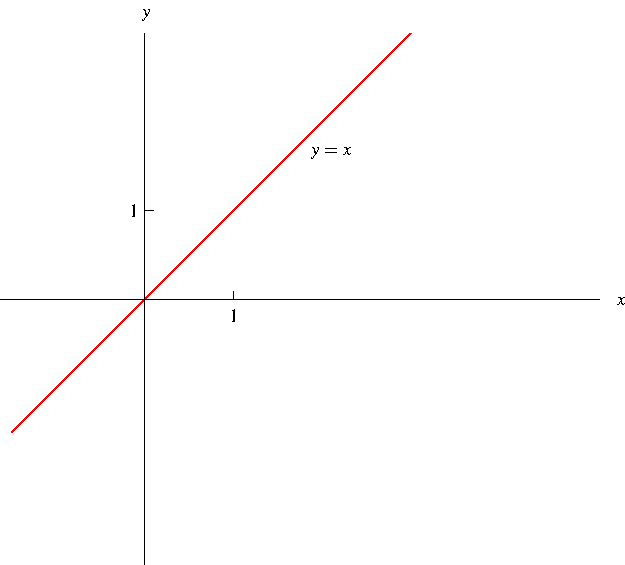
\includegraphics[height=5cm]{../../modules/lines-2d/pictures/01-02-positivea.pdf}%
}%
\only<handout:0| 2>{%
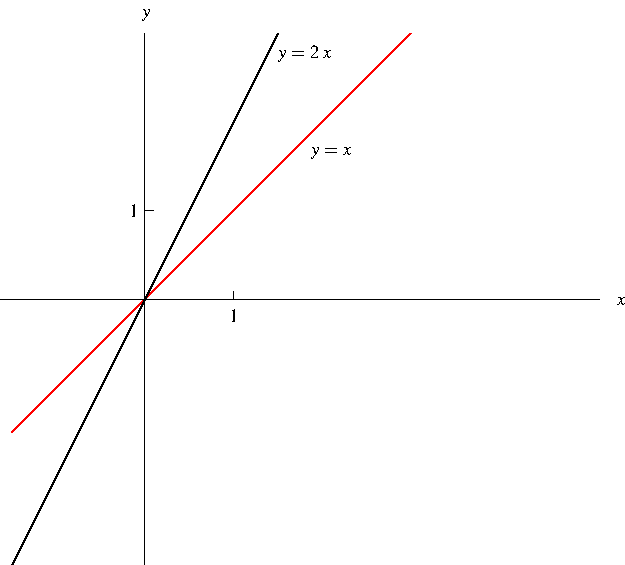
\includegraphics[height=5cm]{../../modules/lines-2d/pictures/01-02-positiveb.pdf}%
}%
\only<handout:0| 3>{%
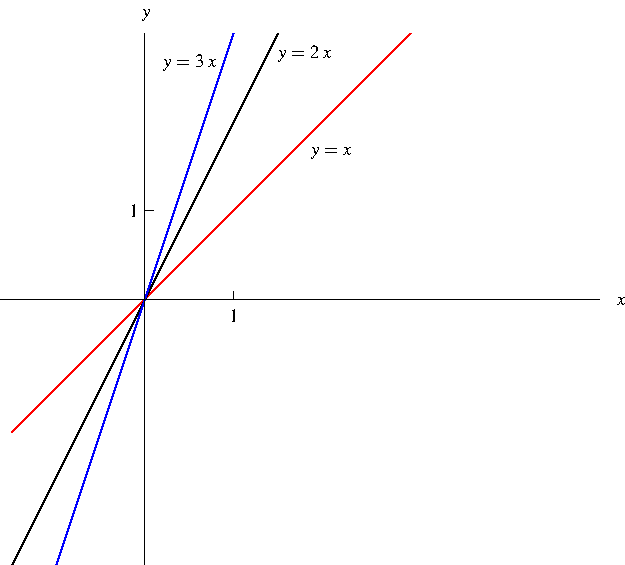
\includegraphics[height=5cm]{../../modules/lines-2d/pictures/01-02-positivec.pdf}%
}%
\only<handout:0| 4>{%
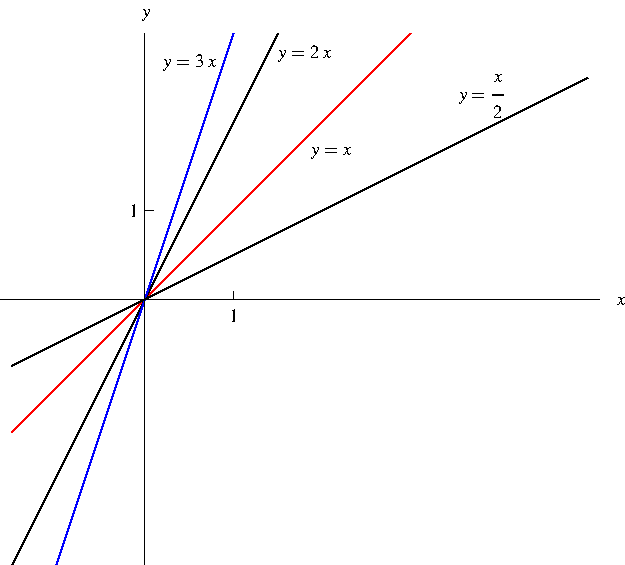
\includegraphics[height=5cm]{../../modules/lines-2d/pictures/01-02-positived.pdf}%
}%
\only<5>{%
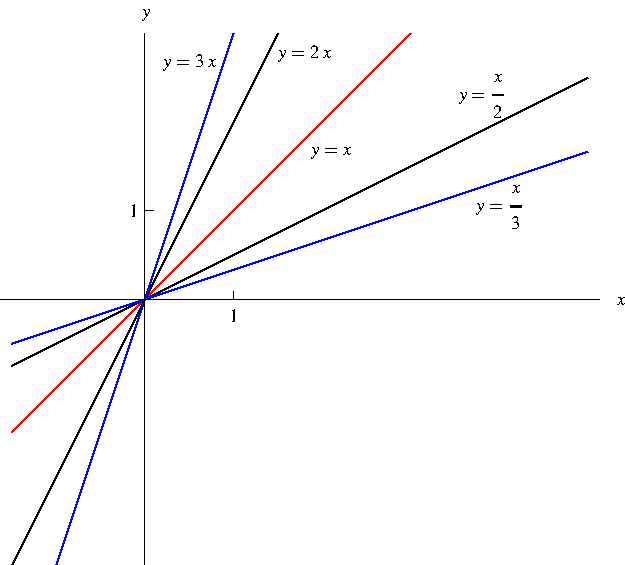
\includegraphics[height=5cm]{../../modules/lines-2d/pictures/01-02-positivee.pdf}%
}%

\begin{itemize}
\item<1->  If two linear functions have positive slopes, the one with the bigger slope increases faster.
\item<2->  $y = 2x$ increases twice as fast as $y = x$.
\item<3->  $y = 3x$ increases three times as fast as $y = x$.
\item<4->  $y = \frac{x}{2}$ increases half as fast as $y = x$.
\item<5->  $y = \frac{x}{3}$ increases one third as fast as $y = x$.
\end{itemize}
\end{frame}

\begin{frame}
\ \only<handout:0| -1>{%
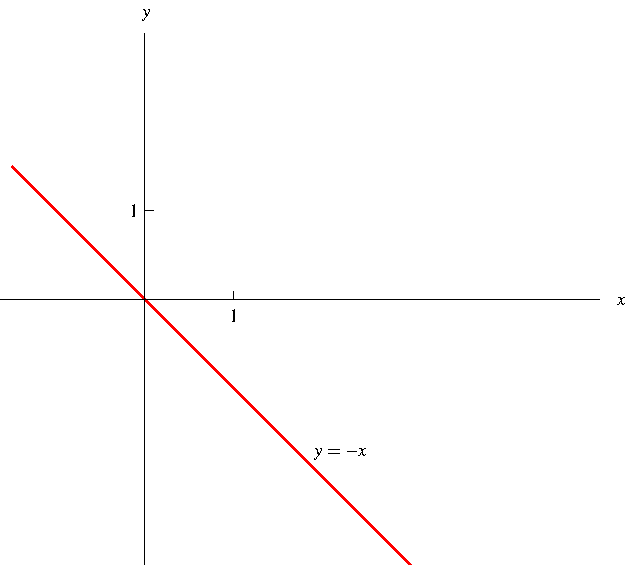
\includegraphics[height=5cm]{precalculus/pictures/01-02-negativea.pdf}%
}%
\only<handout:0| 2>{%
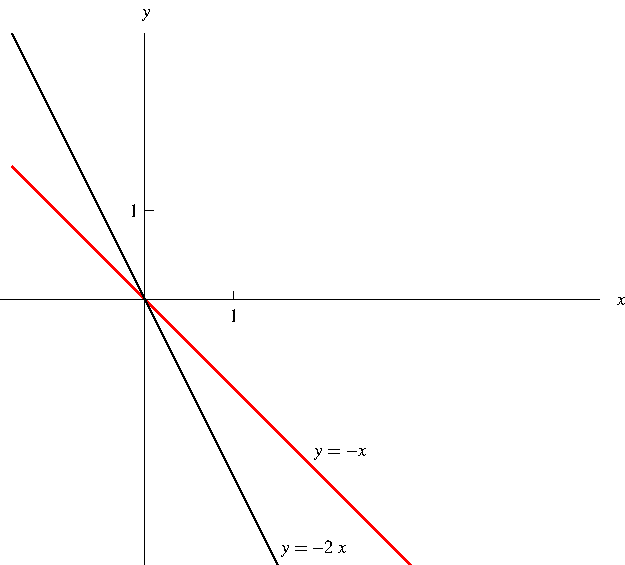
\includegraphics[height=5cm]{precalculus/pictures/01-02-negativeb.pdf}%
}%
\only<handout:0| 3>{%
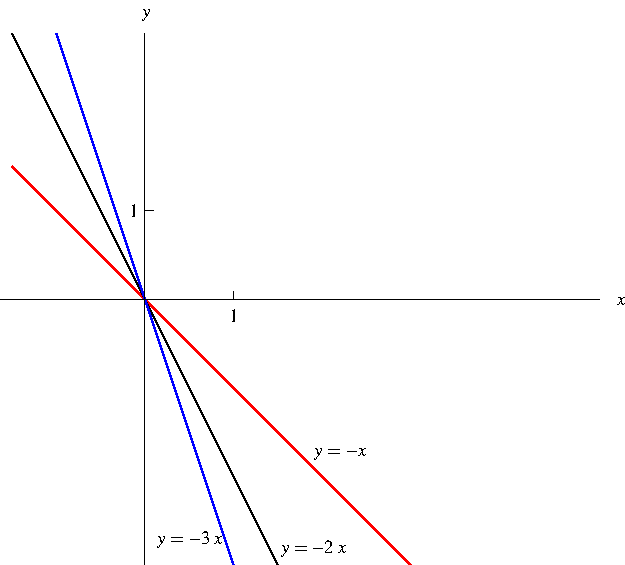
\includegraphics[height=5cm]{precalculus/pictures/01-02-negativec.pdf}%
}%
\only<handout:0| 4>{%
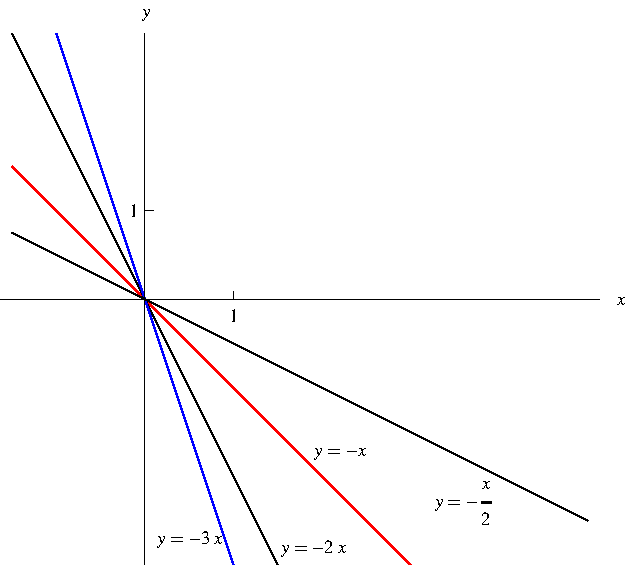
\includegraphics[height=5cm]{precalculus/pictures/01-02-negatived.pdf}%
}%
\only<5>{%
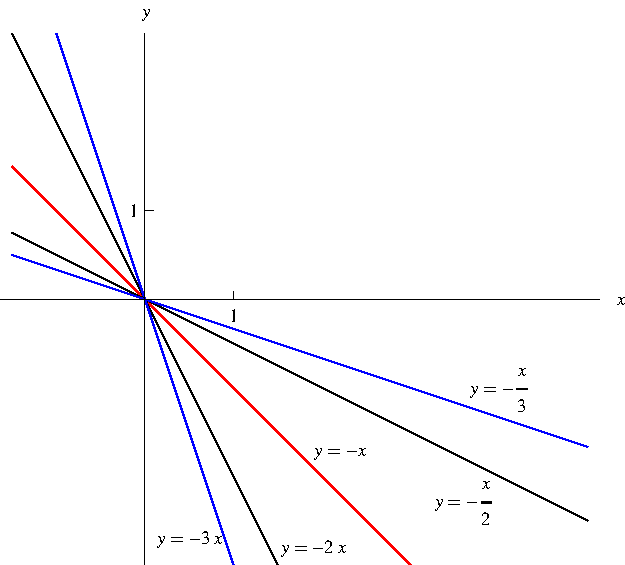
\includegraphics[height=5cm]{precalculus/pictures/01-02-negativee.pdf}%
}%

\begin{itemize}
\item<1->  If two linear functions have negative slopes, the one with the lower slope decreases faster.
\item<2->  $y = -2x$ decreases twice as fast as $y = -x$.
\item<3->  $y = -3x$ decreases three times as fast as $y = -x$.
\item<4->  $y = -\frac{1}{2}x$ decreases half as fast as $y = -x$.
\item<5->  $y = -\frac{1}{3}x$ decreases one third as fast as $y = -x$.
\end{itemize}
\end{frame}
% end module compare-linear


\begin{frame}

\begin{definition}[Vertical line]
A line of the form $x=a$ is called a vertical line.
\end{definition}
\begin{columns}
\column{0.25\textwidth}
\begin{pspicture}(-0.6,-0.6)(2.1,2.1)
\tiny
\fcAxesStandard{-0.5}{-0.5}{2}{2}
\psline[linecolor=\fcColorGraph](1, -0.5)(1,2)
\rput[lt](1.05,-0.05){$a$}
\rput[lt](1.05,1){$(a,y)$}
\fcFullDot{1}{1}
\end{pspicture}
\column{0.75\textwidth}

\begin{itemize}
\item<2-> $y$ does not participate directly in the equation $x=a$.
\item<3-> Therefore the equation cannot be rewritten in slope-intercept form ($y=\textbf{?}x+\textbf{?}$).
\item<4-> Consequently the notion of a slope is not undefined for vertical lines. 
\end{itemize}
\end{columns}
\end{frame}
\begin{frame}
\frametitle{Plotting Lines from line equation}
To plot a line from its equation $ax+by=c$ do the following.
\begin{itemize}
\item<2-> If $b=0 $, the line is vertical through $x=\frac{c}{a}$. \uncover<3->{Suppose $b\neq 0$.}
\begin{itemize}
\item<4-> Plug in arbitrary number for $x$ and find $y$ from $y=\frac{c-ax}{b}$.
\item<5-> Use same procedure to find a second point on the line.
\item<6-> If $a\neq 0$: can also plug in values for $y$ to find $x$.
\item<7-> Draw a line between the two dots. 
\end{itemize}
\end{itemize}
\uncover<7->{
\vskip -0.2cm
\begin{example}
\vskip -0.1cm
\begin{columns}
\column{0.4\textwidth}
\psset{xunit=0.5cm, yunit=0.5cm}
\begin{pspicture}(-4, -4)(5,5)
\tiny
\fcBoundingBox{-4.2}{-4.2}{4.2}{4.2}
\psgrid[subgriddiv=0,griddots=10,gridlabels=0pt](-4,-4)(4,4)
\psaxes[labels=none, arrows=->](0,0)(-4,-4)(4,4)
\fcLabels{4}{4}
\uncover<9-10>{
\fcFullDot{1}{0}
\fcFullDot{0}{1}
}
\uncover<10>{\psline[linecolor=\fcColorGraph](-3,4)(4,-3)}
\uncover<11->{\psline[linecolor=gray](-3,4)(4,-3)}
%
\uncover<12-13>{
\fcFullDot{0}{-3}
\fcFullDot{1.5}{0}
}
\uncover<13>{\psline[linecolor=\fcColorGraph](3.5,4)(-0.5,-4)}
\uncover<14->{\psline[linecolor=gray](3.5,4)(-0.5,-4)}
%
\uncover<15-16>{
\fcFullDot{0}{2}
\fcFullDot{1}{2}
}
\uncover<16>{\psline[linecolor=\fcColorGraph](-4,2)(4,2)}
\uncover<17->{\psline[linecolor=gray](-4,2)(4,2)}
%
\uncover<18-19>{
\fcFullDot{-1}{0}
\fcFullDot{-1}{1}
}
\uncover<19>{\psline[linecolor=\fcColorGraph](-1,-4)(-1,4)}
%\uncover<19>{\psline[linecolor=gray](-3,4)(4,-3)}
\end{pspicture}
\column{0.6\textwidth}
Plot the line with the given equation.
\begin{tabular}{ccc}
equation& pt.  & another pt.\\
$\alertNoH{8-10}{x+y=1}$ & $\fcAnswer{9}{(1,0)}$ &$\fcAnswer{9}{(0,1)}$ \\
$\alertNoH{11-13}{2x-y=3}$& $\fcAnswer{12}{(0,-3)}$ &$\fcAnswer{12}{\left(\frac{3}{2},0\right)}$\\
$\alertNoH{14-16}{y=2}$   & $\fcAnswer{15}{(0,2)}$ &$\fcAnswer{15}{(1,2)}$\\
$\alertNoH{17-19}{x=-1}$  & $\fcAnswer{18}{(-1,0)}$ &$\fcAnswer{18}{(-1,1)}$
\end{tabular}
Other points can be used as well.
\end{columns}
}
\vskip -0.2cm
\end{example}
\end{frame}

\begin{frame}
\begin{example}
Find an equation of a line passing though the indicated pairs of points.
\begin{itemize}
\item $(1,2)$ and $(2,-1)$.
\item $(1,1)$ and $(2,-2)$.
\item $(0,1)$ and $(1,0)$.
\item $(3,5)$ and $(7,-11)$.
\end{itemize}
\end{example}
\end{frame}
\begin{frame}

\begin{example}
Find an equation of the line passing through $(1,2)$ with slope $-\frac{1}{ 2}$.
\end{example}
\end{frame}

\subsection{Line intersection}
\begin{frame}
To find the intersection of two lines  (if they do intersect) with equations $a_1x+b_1y+c_1=0$ and $a_2x+b_2y+c_2=0$ we need to solve the system of equations

\[
\left|\begin{array}{rcl}
a_1x+b_1y+c_1&=&0\\
a_2x+b_2y+c_2&=&0
\end{array}\right.
\]
\end{frame}
\begin{frame}
\begin{example}
Find the intersection of the following lines.
\begin{enumerate}
\item $x-y=3$ and $x+2y=10$.
\item $3x-y=3$ and $x+3y=1$.
\item Line through $(2,0)$ and $(1,2)$ and line through $(3,7 )$ and $(2,5)$.
\item Line through $(3,-1)$ and $(-1, 3)$ and line through $(1,1)$ and $(2,3)$.
\end{enumerate}

\end{example}

\end{frame}
\begin{frame}
\vskip -0.15cm
\begin{definition}
Two lines are parallel if they have no common point.
\end{definition}
\vskip -0.15cm
\begin{proposition}
Two non-vertical lines are parallel if and only if they have equal slopes and different $y$ intercepts.
\end{proposition}
\vskip -0.15cm
\begin{proof}[\only<handout:1|1>{Proof $\Leftarrow$}\only<handout:2|2>{Proof $\Rightarrow$} ]
\only<handout:1|1>{
\begin{itemize}
\item Suppose the two lines have different $y$ intercepts and have the same slope $m$.
\item Then the lines have equations as shown below.
\[
\left|\begin{array}{rcl}
y&=& mx+b_1\\
y&=& mx+b_2
\end{array}\right.
\]
\item System has no solutions as $b_1\neq b_2$ $\Rightarrow$ the lines don't intersect.
\end{itemize}
}
\only<handout:2|2->{
\begin{itemize}
\item Suppose the two lines have different slopes. 
\item Suppose the lines have equations as shown below.
$
\begin{array}{c@{}r@{}c@{}l@{}l|l}
&y&=&m_1x+b_1\\
\cline{1-1}&y&=&m_2x+b_2\\\cline{1-4}
&0&=&(m_1-m_2)x+b_1-b_2\\
&(m_1-m_2)x&=&b_2-b_1 &&\text{Div. by }{m_1-m_2\neq 0}\\
&x&=&\displaystyle \frac{b_2-b_1}{m_1-m_2}
\end{array}
$
\item The system has solution $x=  \frac{b_2-b_1}{m_1-m_2}$, $y= m_1\frac{b_2-b_1}{m_1-m_2}+b_1$ $\Rightarrow$ the lines intersect.
\end{itemize}
}
\vskip -0.7cm
\end{proof}

\vskip 10cm

\end{frame}
}% end lecture

\lect{\semester}{Lecture  4}{4}{
%DesiredLectureName: Functions
\fcLicense
\section{The Definition of a Function}
% begin module function-def
\begin{frame}
\begin{columns}
\column{0.4\textwidth}
\psset{xunit=0.6cm,yunit=0.6cm}
\begin{pspicture}(0,0)(5,5)
\fcBoundingBox{-0.5}{-3.65}{1.1}{3.1}
\rput[r](-1.2,0){$D$}
\uncover<handout:3|6->{
\fcFullDot[scale=2, linecolor=red]{5}{2.5}
\fcFullDot[scale=2, linecolor=red]{0}{2.5}

}
\psellipse*[linecolor=cyan](0,0)(1, 3)
\fcFullDot[scale=1, linecolor=red]{0}{2.5}
\fcFullDot{0}{1.5}
\fcFullDot{0}{0.5}
\fcFullDot{0}{-0.5}
\fcFullDot{0}{-1.5}
\fcFullDot{0}{-2.5}
\uncover<handout:0|4,6>{
\fcFullDot[scale=2, linecolor=red]{0}{-0.5}
}
\uncover<handout:0|4>{
\fcFullDot[scale=2, linecolor=red]{0}{2.5}
\fcFullDot[scale=2, linecolor=red]{0}{1.5}
\fcFullDot[scale=2, linecolor=red]{0}{0.5}
\fcFullDot[scale=2, linecolor=red]{0}{-1.5}
\fcFullDot[scale=2, linecolor=red]{0}{-2.5}
}
\uncover<4->{\rput[t](0, -3.2){\alertNoH{4}
{Domain}}}

\rput[l](6.2,0){$E$}
\psellipse*[linecolor=cyan](5,0)(1, 3)
\fcFullDot[scale=1, linecolor=red]{5}{2.5}
\fcFullDot{5}{1.25}
\fcFullDot{5}{0}
\fcFullDot{5}{-1.25}
\fcFullDot{5}{-2.5}
\fcFullDot{5}{-2.5}
\uncover<handout:0|5,12>{
\fcFullDot[scale=2, linecolor=red]{5}{0}
}
\uncover<handout:0|5,6,9,11>{
\fcFullDot[scale=2, linecolor=red]{5}{2.5}
}
\uncover<handout:0|5,9>{
\fcFullDot[scale=2, linecolor=red]{5}{1.25}
\fcFullDot[scale=2, linecolor=red]{5}{-1.25}
\fcFullDot[scale=2, linecolor=red]{5}{-2.5}
}
\uncover<5->{\rput[t](5, -3.2){\alertNoH{5}{Co-domain}}}
\rput(2.5, 2.5){$f$}
\psline[linestyle=dashed]{->}(0,2.5)(5,1.25)
\psline[linestyle=dashed]{->}(0,1.5)(5,-1.25)
\psline[linestyle=dashed]{->}(0,0.5)(5,-2.5)
\psline[linestyle=dashed]{->}(0,-0.5)(5,2.5)
\psline[linestyle=dashed]{->}(0,-1.5)(5,-1.25)
\psline[linestyle=dashed]{->}(0,-2.5)(5,2.5)
\uncover<handout:3|6->{%
\rput(5.4, 2.5){~~~$f(x)$}
\rput[r](-0.3, -0.5){$x$}
}
\end{pspicture}
\column{0.6\textwidth}
\begin{itemize}
\item<10-> A function has domain $D$ $\Rightarrow$ there is exactly one arrow starting at each element of $D$.
\item<11-> An element of the co-domain can be at the tip of more than one arrow.
\item<12-> It is allowed to have an element in the co-domain without arrows pointing to it.
\end{itemize}
\end{columns}

\begin{definition}[Function]
A function $f$ is a rule that assigns to each element $x$ in a set $D$ exactly one element, called $f(x)$, in a set $E$.
\end{definition}

\only<handout:1| 2-4>{
\begin{itemize}
\item<2-> Functions are also synonymously called ``maps''.
\item<3-> In the picture above, $f$ is represented via the arrows.
\end{itemize}

\uncover<4->{
\begin{definition}[Domain]
The set $D$ in the definition of $f$ is called the domain of $f$. 
\end{definition}
}
}

\only<handout:2| 5>{
\begin{definition}[Co-domain]
The set $E$ in the definition of $f$  is called the co-domain of $f$. 
\end{definition}
}

\only<handout:3| 6-8>{
\begin{definition}[Value of $f$ at $x$]
The number $f(x)$ is called \emph{the value of $f$ at $x$} and is read ``$f$ of $x$''.
\end{definition}

\begin{itemize}
\item<7-> The value of $f$ at $x$ is also called the image of $x$ under the map $f$.
\item<8-> In the expression $f(x)$, $x$ is referred to as the \emph{argument} of $f$. 
\end{itemize}
}
\only<handout:4| 9->{
\begin{definition}[Range]
The set of all possible values taken by $f(x)$ as the element $x$ runs over elements of $D$ is called the range of $f$. 
\end{definition}
}

\vskip 10cm 



\end{frame}
% end module function-def
% begin module function-def
\begin{frame}

\psset{xunit=1.1cm,yunit=1.1cm}
\begin{pspicture}(-1,-1)(4.2,3.1)
\tiny
\psaxes[labels=none, ticks=none]{->}(0,0)(-0.5,-0.5)(4,3)
\rput[r](0,3){$y$}
\rput[l](4,0){$x$}
\psplot[linecolor=red]{0.5}{3}{0.2 x 2 exp mul 0.5 180 x mul sin mul 0.333333 add add
 }
\rput( 3, 2.5){$y=f(x)$}

\only<3>{
\psline[linecolor=red, linewidth=2pt]{<->}(0.5, 0)(3,0)
\rput(1.75, -0.3){\color{red}Domain}
}
\only<4>{
\psline[linecolor=blue, linewidth=2pt]{<->}(0, -0.5)(0,3)
\rput[l](0.05, 2.35){\color{blue}Co-Domain}
}
\only<5>{
\psline[linewidth=1pt](2.166666667, 0)(2.166666667, 1.522222)
\rput[l](2.2,0.7){$f(x)$}
\rput[t](2.2, -0.1){$x$}
}
\only<8>{
\psline[linecolor=purple, linewidth=3pt]{<->}(0, 0.245)(0,2.205)
\rput[l](0.05, 1.1){\color{purple}Range}
\psline[linestyle=dashed](0,0.245)(1.4, 0.245)
\psline[linestyle=dashed](0,2.205)(2.75, 2.205)
}
\end{pspicture}
\begin{definition}[Function]
A function $f$ is a rule that assigns to each element $x$ in a set $D$ exactly one element, called $f(x)$, in a set $E$.
\end{definition}

\only<handout:1| 2-3>{
\begin{itemize}
\item Functions are also synonymously called ``maps''.
\end{itemize}

\uncover<3->{
\begin{definition}[Domain]
The set $D$ in the definition of $f$ is called the domain of $f$. 
\end{definition}
}
}

\only<handout:2| 4>{
\begin{definition}[Co-domain]
The set $E$ in the definition of $f$  is called the co-domain of $f$. 
\end{definition}
}
\only<handout:3| 5-7>{
\begin{definition}[Value of $f$ at $x$]
The number $f(x)$ is called \emph{the value of $f$ at $x$} and is read ``$f$ of $x$''.
\end{definition}

\begin{itemize}
\item<6-> The value of $f$ at $x$ is also called the image of $x$ under the map $f$.
\item<7-> In the expression $f(x)$, $x$ is referred to as the \emph{argument} of $f$. 
\end{itemize}
}
\only<handout:4| 8->{
\begin{definition}[Range]
The set of all possible values taken by $f(x)$ as the element $x$ runs over elements of $D$ is called the range of $f$. 
\end{definition}
}


\vskip 10cm 


\end{frame}
% end module function-def
\begin{frame}
\begin{itemize}
\item The notation $f(x)$ for the image of $x$ was introduced by Leonhard Euler.
\item<2-> Expressions such as $a(x+y)$ may either refer to
\begin{itemize}
\item<3-> the function $a$ applied to the argument $x+y$ or
\item<4-> the number $a$ multiplied by $x+y$.
\end{itemize}
\item<5-> Which of the two cases is at hand should be clarified with English language. 
\item<6-> However if no such clarification is present (as often is the case in mathematical exercises/tests), the matter is up to the reader's intelligent interpretation.
\end{itemize}
\end{frame}
\begin{frame}
\frametitle{Functions via formulas}
\begin{itemize}
\item When we want to define a function $f$ whose domain (input) is a number, we often use algebraic formulas, for example:
\[
f(\only<handout:1,2|-16>{ {\color{blue}x}} \only<handout:3|17->{ {\color{purple}t}} )=2{{\only<handout:1,2|-16>{\color{blue}x}} {\only<handout:3|17->{\color{purple}t}} }^2+ \only<handout:1,2|-16>{{\color{blue}x}} \only<handout:3|17->{{\color{purple}t}}+ 1.
\]
\item<2-> In the notation above, ${\color{blue}x}$ is an \alertNoH{6}{independent}, \alertNoH{8}{bounded (dummy, placeholder)} variable - it denotes a substitution pattern. 
\only<handout:1|1-6>{
\item<3-> We could think of ${\color{blue}x}$ as a placeholder - instead of $f({\color{blue}x})=2{\color{blue}x}^2+{\color{blue}x}+1$ we could write $f({\color{blue}\Box}) = 2 {\color{blue}\Box} ^2 + {\color{blue}\Box}+1$. 
\item<4-> Here, ${\color{blue}\Box}$ denotes our ability to substitute $f({\color{blue}\Box})$ by $2{\color{blue}\Box}^2+{\color{blue}\Box}+1$.
\item<5-> For example $f(\alertNoH{5}{1})=2\cdot \alertNoH{5}{1}^2+\alertNoH{5}{1}+1$. 
\item<6-> The word \alertNoH{6}{independent} refers to the fact that ${\color{blue}x}$ is no relation with any of the other variables in the text.
}
\only<handout:2|7->{
\item Another example is $f({\color{red}x}^2)= 2 \left({\color{red}x}^2\right)^2+{\color{red}x}^2+1$.
}
\only<handout:2|8-13>{
\item This example illustrates the meaning of the word \alertNoH{8}{bounded (dummy, placeholder)}: \uncover<9->{the dummy variable ${\color{blue}x}$ is only a convenient placeholder label,} \uncover<10->{and is a distinct mathematical object from the variable ${\color{red}x}$ which has meaning outside of the expression $f({\color{red}x}^2)$.} 
\item<11-> If we omit the clarification colors, it is no longer clear whether $f(x)$ refers to the defining expression for $f({\color{blue}x})$, \uncover<12->{or to an expression $f({\color{red}x})$ where ${\color{red}x}$ has meaning outside of the definition of $f$.}
}
\only<handout:3|13->{
\item Computer algebra systems will ``keep track of the colors'' and will not confuse the dummy ${\color{blue}x}$ with the non-dummy variable ${\color{red}x} $.
}
\only<handout:3|14->{
\item<15-> For humans however the danger of confusion is real. 
\item<16-> In case of human confusion, clarification should be sought through \alertNoH{16,17}{renaming variables}, \alertNoH{17}{as illustrated above}.
\item<18-> The relabeling of the dummy variable to ${\color{purple}{t}}$ removes any confusion about the meaning of $f({\color{red}x}^2)$.
\item<19-> In computer programming, the issues described here are addressed via ``variable scope rules''.
}
\end{itemize}

\vskip 10cm
\end{frame}
\begin{frame}
\begin{example}
Let $\alertNoH{2,4}{ f{}({\alertNoH{3,5}{x}})=\alertNoH{3,5}{x}^2- \alertNoH{3,5}{x}-1}$.  Evaluate the difference quotient and \alertNoH{6,13}{simplify your answer}. 
\[
\begin{array}{rcl}
\displaystyle \frac{\alertNoH{2}{ f{}(\alertNoH{3}{2+h})} - \alertNoH{4}{f{}(\alertNoH{4}{2})} }{h}&=&\displaystyle \uncover<2->{\frac{\left( \alertNoH{2}{ \alertNoH{6,7}{ (\alertNoH{3}{2+h})^2} \alertNoH{8}{-}(\alertNoH{3}{2+h})-1} \right) \alertNoH{9}{-} (\alertNoH{4}{\alertNoH{5}{2}^2 \alertNoH{9}{-}\alertNoH{5}{2}\alertNoH{9}{-} 1})}{h}}\\
\uncover<6->{ &=&\displaystyle \frac{ \fcAnswer{7}{\fcCancel{10}{ 2^2} + \alertNoH{11}{2\cdot 2 h} +h^2} \alertNoH{8}{-}\fcCancel{10}{2} \alertNoH{11}{\alertNoH{8}{-}h}-\fcCancel{10}{1} \alertNoH{9}{-} \fcCancel{10}{2^2} \alertNoH{9}{+} \fcCancel{10}{2} \alertNoH{9}{+}\fcCancel{10}{1}}{h} }\\
\uncover<11->{&=&\displaystyle \frac{h^2 + \alertNoH{11}{3h} }{h}}\\
\uncover<12->{&=&\displaystyle \frac{\fcCancel{13}{h}(h+3)}{\fcCancel{13}{h}}}\\
\uncover<13->{&=&\displaystyle h+3}\\
\end{array}
\]


\end{example}
\end{frame}
\subsection{Function Domains}
% begin module domains
\begin{frame}
\frametitle{A Note on Domains of Functions}
If the domain of a function isn't specified, it is implied to be all numbers $x$ for which the formula $f(x)$ is defined. There are some restrictions to consider:
\begin{itemize}
\item<2->  Can't divide by $0$.
\item<3->  Even roots of a negative number are not defined in this course ($\sqrt{-1} , \sqrt[4]{-2053}, \sqrt[6]{-15} \ldots$ not allowed).
\item<4->  Taking $\log x$ if $x \leq 0$ is not allowed in this course; taking  $\log 0$ is not allowed in any course.
\end{itemize}
\end{frame}


% end module domains

\begin{frame}
\begin{example}
Find the implied domains of the given functions.
\begin{columns}
\column{.5\textwidth}
\[
f(x) = \alertNoH{ 5}{\sqrt[4]{x-2}} + \sqrt[3]{6-x}
\]
\begin{itemize}
\item<2->  Any risk of dividing by $0$?  \uncover<3->{No.}
\item<4->  Any risk of taking the even root of a negative number? \uncover<5->{\alertNoH{ 5}{Yes.}}
\item<6->  $x - 2$  must not be negative.
\end{itemize}
\begin{eqnarray*}
\uncover<7->{x - 2} & \uncover<7->{\geq} & \uncover<7->{0}\\
\uncover<8->{x} & \uncover<8->{\geq} & \uncover<8->{2}
\end{eqnarray*}
\uncover<9->{Domain is all real numbers greater than or equal to $2$; that is, $[2,\infty )$.
}%
\column{.5\textwidth}
\[
g(x) = \frac{x^2 - 9}{\alertNoH{ 11}{x^2 - x - 6}}
\]
\begin{itemize}
\item<10->  Any risk of dividing by $0$?  \uncover<11->{\alertNoH{ 11}{Yes.}}
\item<12->  Any risk of taking the even root of a negative number? \uncover<13->{No.}
\item<14->  $x^2 - x - 6$ must not equal $0$.
\end{itemize}
\abovedisplayskip=0pt
\belowdisplayskip=0pt
\abovedisplayshortskip=0pt
\belowdisplayshortskip=0pt
\begin{eqnarray*}
\uncover<15->{x^2 - x - 6} & \uncover<15->{\neq} & \uncover<15->{0}\\
\uncover<16->{(x - 3)(x + 2)} & \uncover<16->{\neq} & \uncover<16->{0}\\
\uncover<17->{x} & \uncover<17->{\neq} & \uncover<17->{3 \text{ or } -2}\\
\end{eqnarray*}
\uncover<18->{Domain is all real numbers except $3$ and $-2$; that is, \\ $(-\infty , -2)$ $\cup (-2,3)$ $\cup (3,\infty )$.
}%
\end{columns}
\end{example}
\end{frame}

\subsection{The Vertical Line Test}
% begin module vertical-line-test
\begin{frame}
\frametitle{The Vertical Line Test}
\begin{question}
Given a curve in the plane, is it the graph of a function or not?
\end{question}

\uncover<2->{The answer is as follows.
\begin{proposition}[The Vertical Line Test]
A curve in the plane is the graph of a function if and only if no vertical line intersects it more than once.
\end{proposition}
}

\begin{tabular}{ccc}
\psset{xunit=0.35cm, yunit=0.35cm}
\begin{pspicture}(-5, -5)(5,5) 
\psframe*[linecolor=white](-5,-5)(5,5) 
\psaxes[ticks=none, labels=none]{<->}(0,0)(-4.5,-4.5)(4.5,4.5)\tiny
%Function formula: sin{}(x) 
\psplot[linecolor=red, plotpoints=1000]{-5}{5}{x 57.29578 mul sin }
\end{pspicture}
%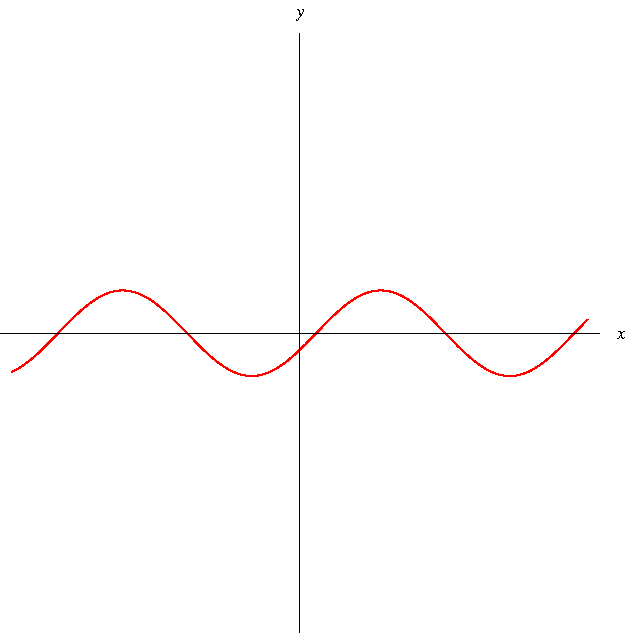
\includegraphics[height=3.8cm]{precalculus/pictures/01-02-vlt3.pdf} 
&%
\psset{xunit=0.35cm, yunit=0.35cm}
\begin{pspicture}(-5, -5)(5,5) \psframe*[linecolor=white](-5,-5)(5,5) 
\psaxes[ticks=none, labels=none]{<->}(0,0)(-4.5,-4.5)(4.5,4.5)\parametricplot[linecolor=red, plotpoints=1000]{0.05}{3}{t t 2.2 mul 57.29578 mul sin 1 add add t 57.29578 mul cos mul t t 2.2 mul 57.29578 mul sin 1 add add t 57.29578 mul sin mul}
\only<handout| 6->{%
\psline(1.7, -4.5)(1.7, 4.5)
}
\end{pspicture}
%\only<handout:0| -2>{%
%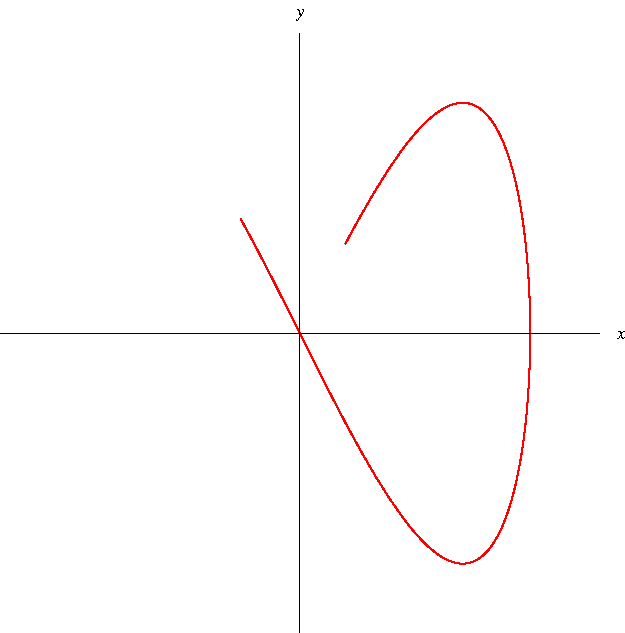
\includegraphics[height=3.8cm]{precalculus/pictures/01-02-vlt1a.pdf}%
%}%
%\only<handout| 3->{%
%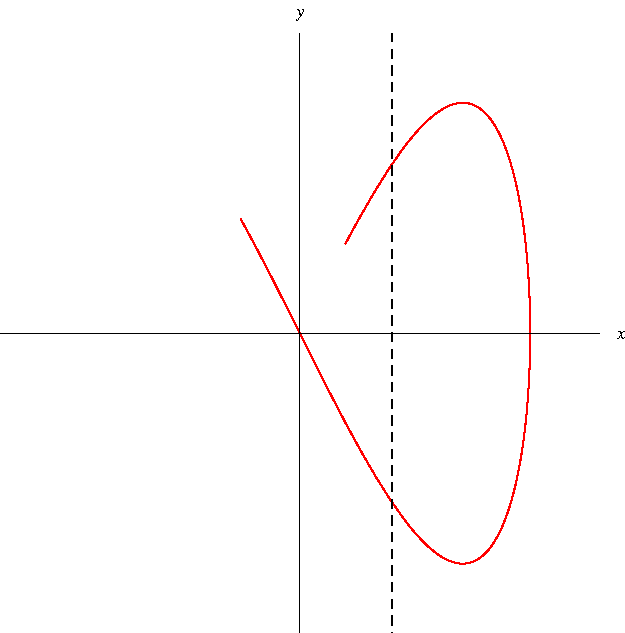
\includegraphics[height=3.8cm]{precalculus/pictures/01-02-vlt1b.pdf}%
%} 
&%
\psset{xunit=0.35cm, yunit=0.35cm}
\begin{pspicture}(-5, -5)(5,5) 
\psframe*[linecolor=white](-5,-5)(5,5) 
\psaxes[ticks=none, labels=none]{<->}(0,0)(-4.5,-4.5)(4.5,4.5)\tiny
%Function formula: 3/8+3/2 ((x)^{2})+1/4 (x)- ((x)^{3}) 
\psplot[linecolor=red, plotpoints=1000]{-0.5}{2}{x 3 exp -1 mul x 0.25 mul x 2 exp 1.5 mul 0.375 add add add } %Function formula: 1+1/2 (x) 
\psplot[linecolor=red, plotpoints=1000]{-4}{-0.5}{x 0.5 mul 1 add }
\end{pspicture} 
%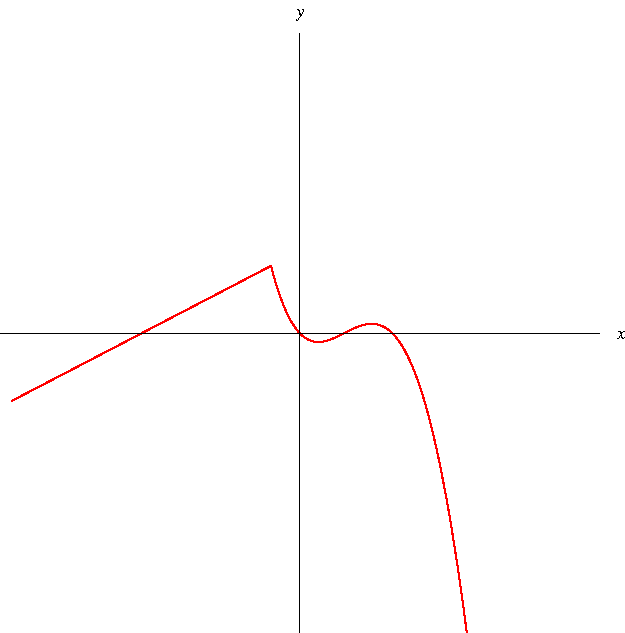
\includegraphics[height=3.8cm]{precalculus/pictures/01-02-vlt2.pdf} 
\\%
\fcAnswerUncoverNoH{1}{4}{Function} &
\fcAnswerUncoverNoH{1}{6}{Not a function}&
\fcAnswerUncoverNoH{1}{8}{Function}
\end{tabular}
\end{frame}
% end module vertical-line-test

\subsection{Piecewise Defined Functions}
% begin module function-piecewise
\begin{frame}
\frametitle{Piecewise Defined Functions}
\begin{definition}[Piecewise Defined Function]
A piecewise defined function is a function that is defined by different algebraic formulas on different subsets of its domain.
\end{definition}
\uncover<2->{
\begin{example}
\begin{columns}[t]
\column{.4\textwidth}
\ 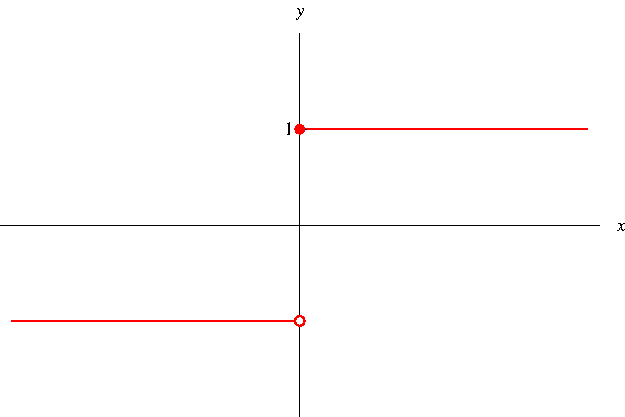
\includegraphics[height=3.5cm]{precalculus/pictures/01-01-piecewise.pdf}
\column{.5\textwidth}
\[
f(x) = \left\{ \begin{array}{rcc}
1 & \textrm{ if } & x \geq 0 \\
-1 & \textrm{ if } & x < 0 
\end{array}\right. 
\]

The filled red circle means $(0,1)$ is on the curve.  

The open circle means $(0, -1)$ is not on the curve.
\end{columns}
\end{example}
}
\end{frame}
% end module function-piecewise

% begin module absolute-value 
\begin{frame}
\begin{example}[Example 8, p. 18]
The absolute value $|a|$ of a number $a$ is defined to be
\[
|a| = \left\{ \begin{array}{ccccl}
\alert<handout:0| 2-3>{a} & \alert<handout:0| 3>{\textrm{if}} & \alert<handout:0| 3>{ a} & \alert<handout:0| 3>{\geq} & \alert<handout:0| 3>{0} \\
\alert<handout:0| 4-5>{-a} & \alert<handout:0| 5>{\textrm{if}} &  \alert<handout:0| 5>{a} & \alert<handout:0| 5>{<} & \alert<handout:0| 5>{0}. \end{array}\right.
\]

Sketch a graph of the function $f(x) = |x|$.

\begin{center}
\ \only<handout:0| 1>{%
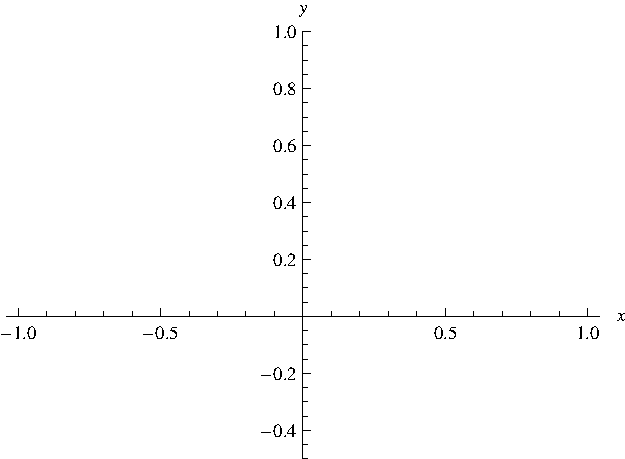
\includegraphics[height=4cm]{precalculus/pictures/01-01-ex-08a.pdf}%
}%
\only<handout:0| 2>{%
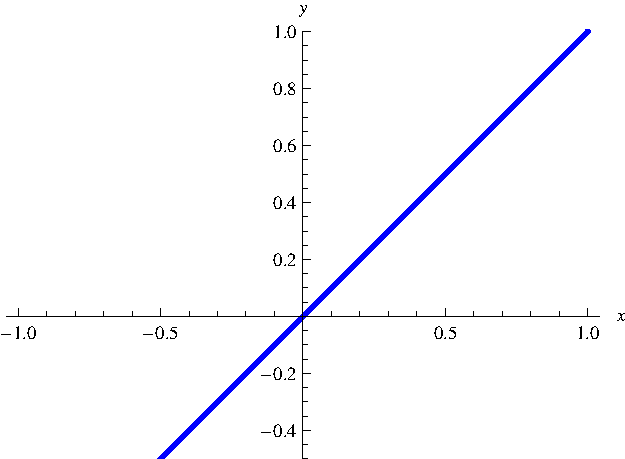
\includegraphics[height=4cm]{precalculus/pictures/01-01-ex-08b.pdf}%
}%
\only<handout:0| 3>{%
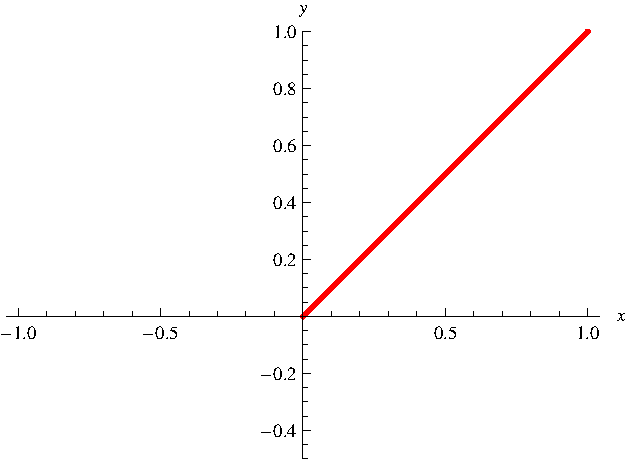
\includegraphics[height=4cm]{precalculus/pictures/01-01-ex-08c.pdf}%
}%
\only<handout:0| 4>{%
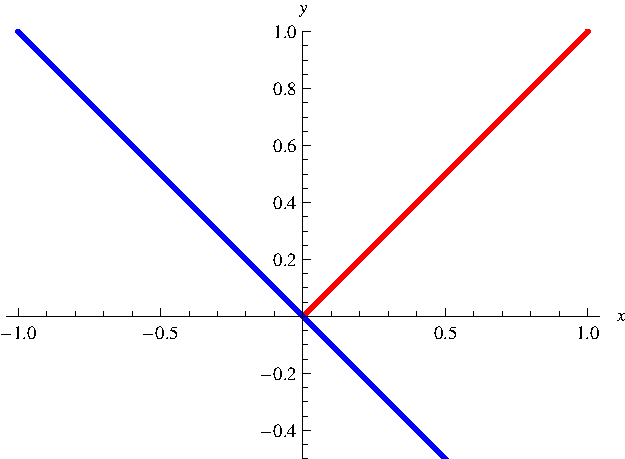
\includegraphics[height=4cm]{precalculus/pictures/01-01-ex-08d.pdf}%
}%
\only<handout:1-| 5>{%
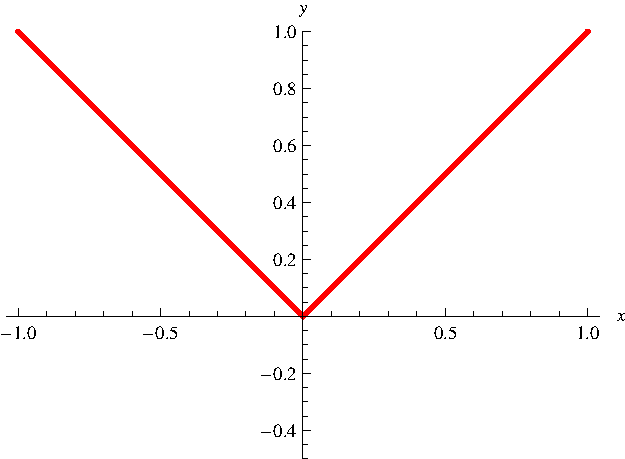
\includegraphics[height=4cm]{precalculus/pictures/01-01-ex-08e.pdf}%
}%
\end{center}
\end{example}
\end{frame}
% end module absolute-value 

% begin module piecewise-formula
\begin{frame}
\begin{example} %[Example 9, p. 18]
Find a formula for the function $f$ in the graph.

\psset{xunit=1.2cm, yunit=1.2cm}
\begin{pspicture}(-4, -0.5)(4,4) 
\tiny
\psframe*[linecolor=white](-5,-5)(5.2,5.2) 
\psaxes{<->}(0,0)(-0.5,-0.5)(5.2,2.2)
\psLabels{5.1}{2.2}
\psline[linecolor=red](0,0)(1,1)(2,0)(5,0)
\psHollowDot{5}{0}
\psFullDot{0}{0}
\only<4-5>{
\psline[linecolor=blue](-0.5, -0.5)(2,2)
}
\only<6-7>{
\psline[linecolor=blue](-0.2, 2.2)(2.5,-0.5)
}
\only<8-9>{
\psline[linecolor=blue](2, 0)(5,0)
}
\end{pspicture} 
%\ \only<1-3,10>{%
%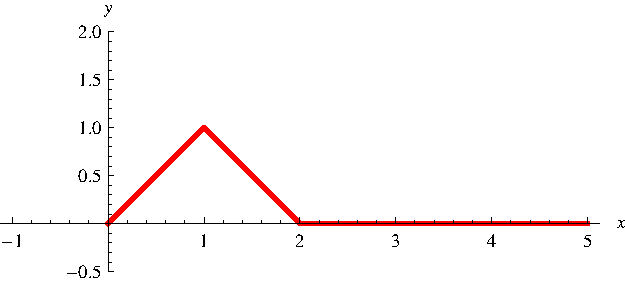
\includegraphics[height=4cm]{precalculus/pictures/01-01-ex-09a.pdf}%
%}%
%\only<handout:0| 4-5>{%
%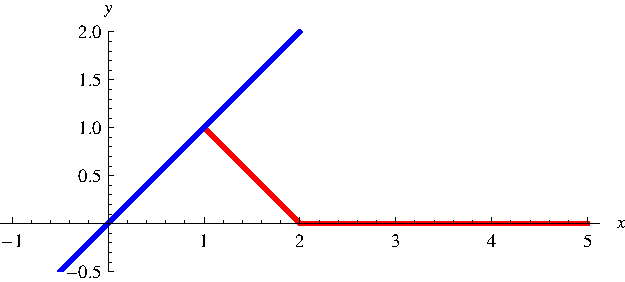
\includegraphics[height=4cm]{precalculus/pictures/01-01-ex-09b.pdf}%
%}%
%\only<handout:0| 6-7>{%
%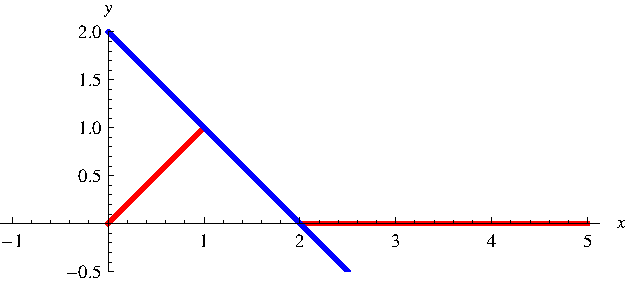
\includegraphics[height=4cm]{precalculus/pictures/01-01-ex-09c.pdf}%
%}%
%\only<handout:0| 8-9>{%
%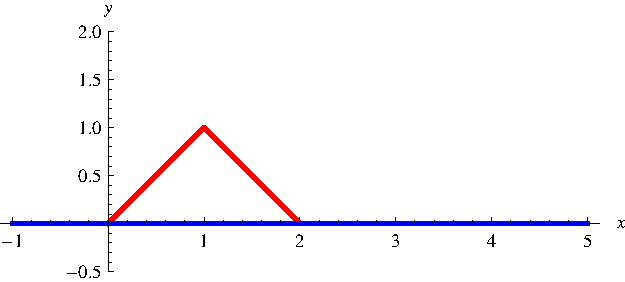
\includegraphics[height=4cm]{precalculus/pictures/01-01-ex-09d.pdf}%
%}%

\uncover<2->{
Different formulas on $[0, 1)$, $[1, 2)$, and $[2, 5)$. 
}

\uncover<3->{
\[
f(x) = \left\{ \begin{array}{ccccccl}
\uncover<5->{\alert<handout:0| 5>{x}} & \alert<handout:0| 4-5>{\textrm{if}} & \alert<handout:0| 4-5>{0} & \alert<handout:0| 4-5>{\leq} & \alert<handout:0| 4-5>{x} & \alert<handout:0| 4-5>{<} & \alert<handout:0| 4-5>{1} \\
\uncover<7->{\alert<handout:0| 7>{2 - x}} & \alert<handout:0| 6-7>{\textrm{if}} & \alert<handout:0| 6-7>{1} & \alert<handout:0| 6-7>{\leq} & \alert<handout:0| 6-7>{x} & \alert<handout:0| 6-7>{<} & \alert<handout:0| 6-7>{2} \\
\uncover<9->{\alert<handout:0| 9>{0}} & \alert<handout:0| 8-9>{\textrm{if}} & \alert<handout:0| 8-9>{2} & \alert<handout:0| 8-9>{\leq} & \alert<handout:0| 8-9>{x} & \alert<handout:0| 8-9>{<} & \alert<handout:0| 8-9>{5} \end{array}\right.
\]
}
\end{example}
\end{frame}
% end module piecewise-formula

% begin module piecewise-ex1
\begin{frame}
\begin{example}
Sketch the function $f(x)  = |2x-3|$.
\begin{columns}
\column{.4\textwidth}
\psset{xunit=1.6cm, yunit=1.6cm}
\begin{pspicture}(-0.5, -0.5)(2.8,2.8)
\tiny
\psframe*[linecolor=white](-0.5,-0.5)(2.8,2.8)
\psaxes{<->}(0,0)(-0.5,-0.5)(2.75,2.5)
\fcLabels{2.75}{2.5}
\uncover<6->{
\psline[linecolor=red](1.5, 0)(2.75,2.5)
}
\uncover<7->{
\psline[linecolor=red](0.25,2.5)(1.5, 0)
}
\end{pspicture}
%\only<-5| handout:0>{%
%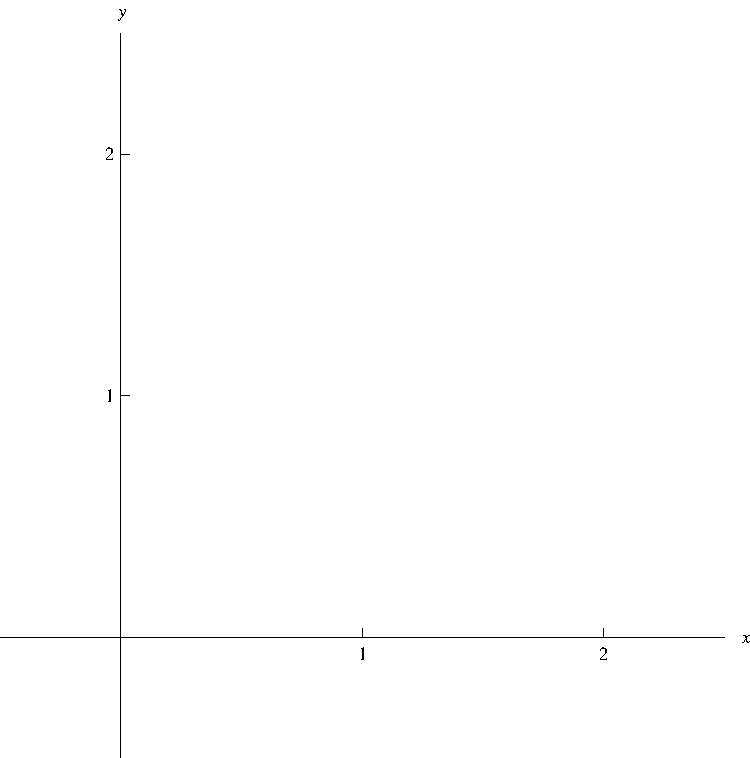
\includegraphics[width=4.5cm]{precalculus/pictures/piecewise-ex1-1.pdf}%
%}%
%\only<6| handout:0>{%
%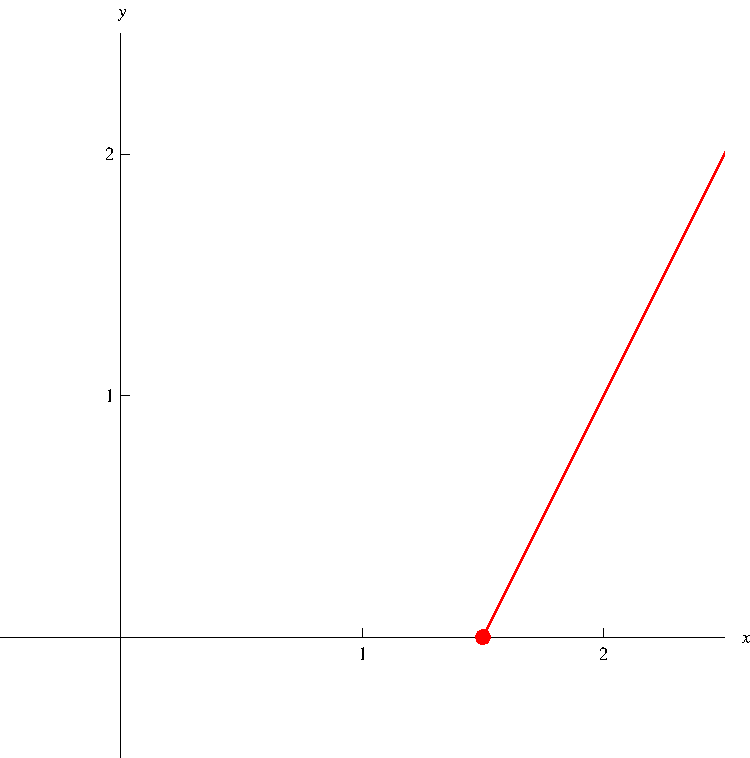
\includegraphics[width=4.5cm]{precalculus/pictures/piecewise-ex1-2.pdf}%
%}%
%\only<7-| handout:1>{%
%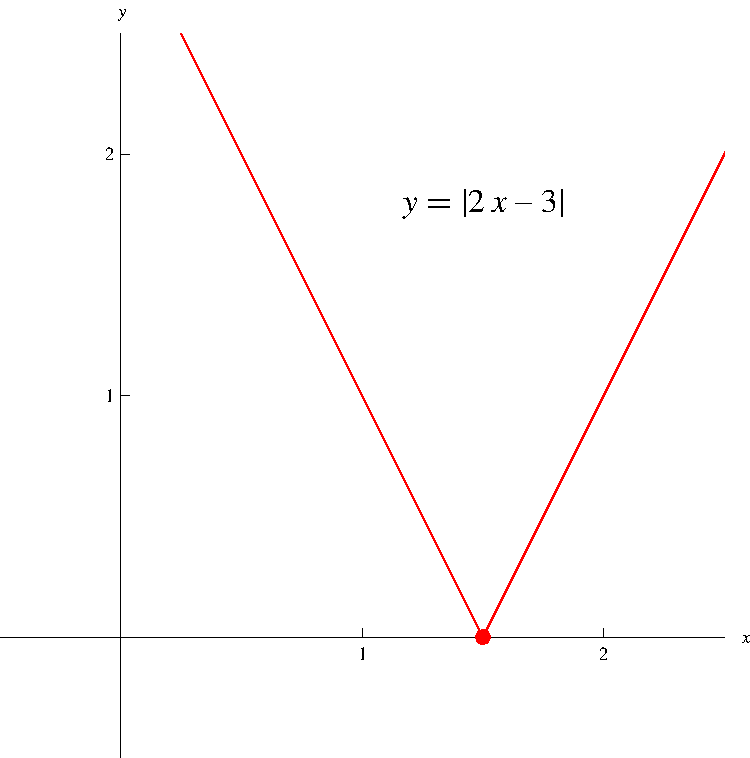
\includegraphics[width=4.5cm]{precalculus/pictures/piecewise-ex1-3.pdf}%
%}%
\column{.55\textwidth}
\abovedisplayskip=0pt
\belowdisplayskip=-15pt
\abovedisplayshortskip=0pt
\belowdisplayshortskip=0pt
\begin{align*}
\uncover<2->{%
|\alert<handout:0| 3>{x}| %
}%
& \uncover<2->{%
 = \begin{cases}
\alert<handout:0| 3>{x} & \text{if $\alert<handout:0| 3>{x} \geq 0$}\\
-\alert<handout:0| 3>{x} & \text{if $\alert<handout:0| 3>{x} < 0$}.\\
\end{cases}
}\\%
\uncover<3->{%
|\alert<handout:0| 3>{2x-3}| %
}%
& \uncover<3->{%
 = \begin{cases}
\alert<handout:0| 3>{2x-3} & \text{if $\alert<handout:0| 3>{2x-3} \geq 0$}\\
-(\alert<handout:0| 3>{2x-3}) & \text{if $\alert<handout:0| 3>{2x-3} < 0$}\\
\end{cases}
}\\%
& \uncover<4->{%
 = \begin{cases}
2x-3 & \text{if $2x \geq 3$}\\
-2x+3 & \text{if $2x < 3$}\\
\end{cases}
}\\%
& \uncover<5->{%
 = \begin{cases}
\alert<handout:0| 6>{2x-3} & \alert<handout:0| 6>{\text{if $x \geq 3/2$}}\\
\alert<handout:0| 7>{-2x+3} & \alert<handout:0| 7>{\text{if $x < 3/2$}}.\\
\end{cases}
}%
\end{align*}
\end{columns}
\end{example}
\end{frame}
% end module piecewise-ex1

% begin module piecewise-ex2
\begin{frame}
\begin{example}
Sketch the function $\displaystyle f(x)  = \frac{|4x+2|}{2x+1}$.
\begin{columns}
\column{.4\textwidth}
\psset{xunit=1cm, yunit=1cm}
\begin{pspicture}(-4, -0.5)(4,4) 
\tiny
\psframe*[linecolor=white](-5,-5)(5.2,5.2) 
\psaxes{<->}(0,0)(-3.2,-3.2)(2.2,3.2)
\psLabels{2.2}{3.2}
\uncover<9->{
\psline[linecolor=red](-0.5, 2)(2.2,2)
\psHollowDot{-0.5}{2}
}
\uncover<10->{
\psline[linecolor=red](-0.5,-2)(-3, -2)
\psHollowDot{-0.5}{-2}
}
\end{pspicture} 
%\only<-8| handout:0>{%
%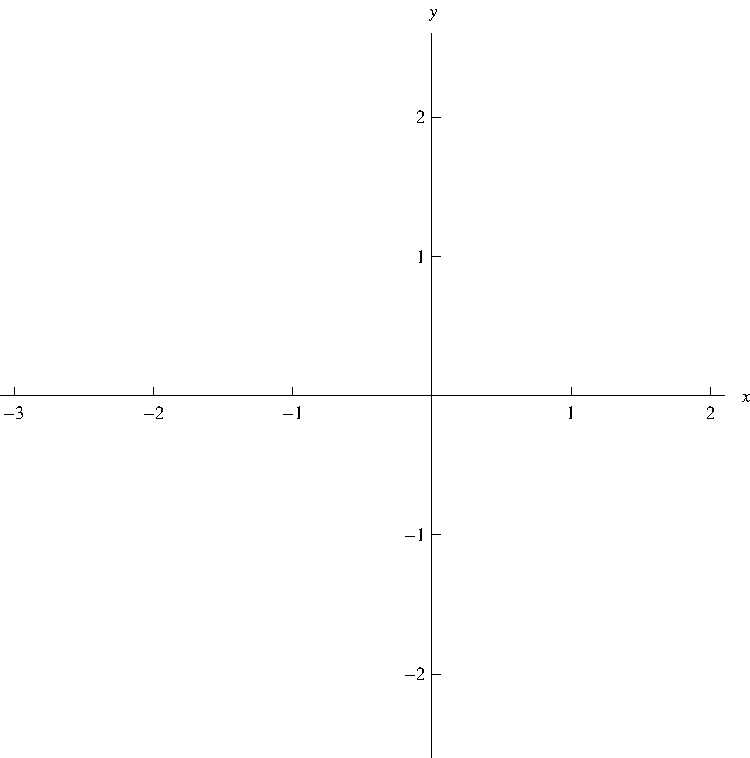
\includegraphics[width=4.5cm]{precalculus/pictures/piecewise-ex2-1.pdf}%
%}%
%\only<9| handout:0>{%
%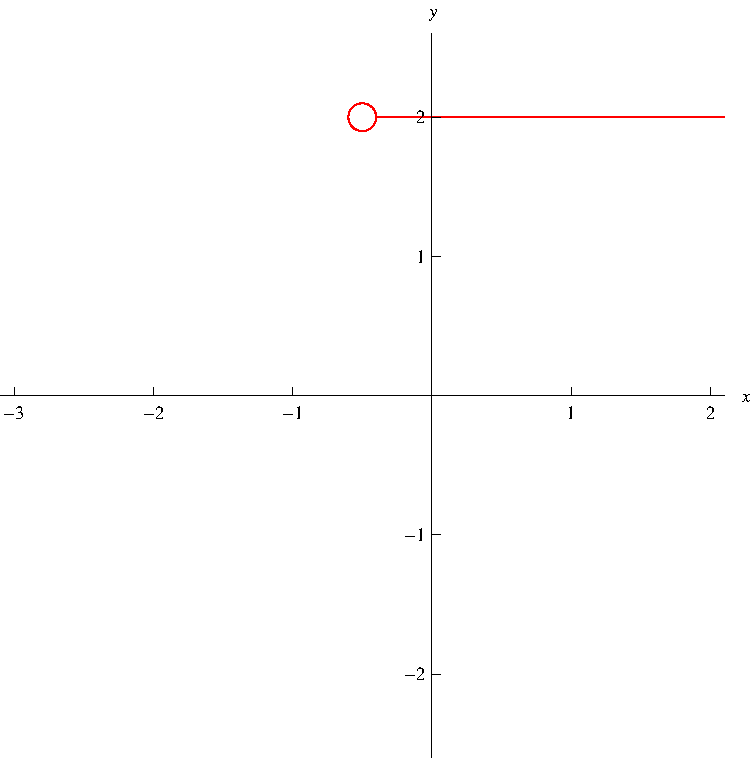
\includegraphics[width=4.5cm]{precalculus/pictures/piecewise-ex2-2.pdf}%
%}%
%\only<10-| handout:1>{%
%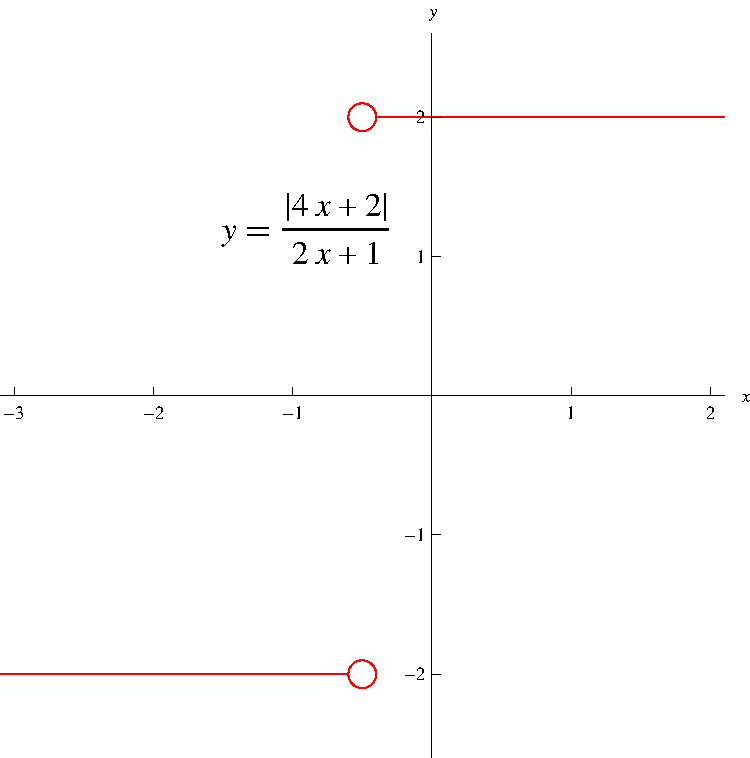
\includegraphics[width=4.5cm]{precalculus/pictures/piecewise-ex2-3.pdf}%
%}%
\column{.55\textwidth}
\abovedisplayskip=0pt
\belowdisplayskip=-15pt
\abovedisplayshortskip=0pt
\belowdisplayshortskip=0pt
\begin{align*}
\uncover<2->{%
|\alert<handout:0| 3>{x}| %
}%
& \uncover<2->{%
 = \begin{cases}
\alert<handout:0| 3>{x} & \text{if $\alert<handout:0| 3>{x} \geq 0$}\\
-\alert<handout:0| 3>{x} & \text{if $\alert<handout:0| 3>{x} < 0$}.\\
\end{cases}
}\\%
\uncover<3->{%
\frac{|\alert<handout:0| 3>{4x+2}|}{2x+1} %
}%
& \uncover<3->{%
 = \begin{cases}
\frac{\alert<handout:0| 3-5>{4x+2}}{2x+1} & \text{if $\alert<handout:0| 3>{4x+2} > 0$}\\
\frac{\alert<handout:0| 6-7>{-(\alert<handout:0| 3>{4x+2})}}{2x+1} & \text{if $\alert<handout:0| 3>{4x+2} < 0$}\\
\end{cases}
}\\%
& \uncover<4->{%
 = \begin{cases}
\frac{\uncover<5->{\alert<handout:0| 5>{2(2x+1)}}}{2x+1} & \text{if $4x > -2$}\\
\frac{\uncover<7->{\alert<handout:0| 7>{-2(2x+1)}}}{2x+1} & \text{if $4x < -2$}\\
\end{cases}
}\\%
& \uncover<8->{%
 = \begin{cases}
\alert<handout:0| 9>{2} & \alert<handout:0| 9>{\text{if $x > -1/2$}}\\
\alert<handout:0| 10>{-2} & \alert<handout:0| 10>{\text{if $x < -1/2$}}.\\
\end{cases}
}%
\end{align*}
\end{columns}
\end{example}
\end{frame}
% end module piecewise-ex2

\subsection{Zeroes of a function}
\begin{frame}

\begin{definition}
The zeroes of a function $f$ are the values of the argument $x$ for which $f(x)=0$.
\end{definition}

\begin{observation}
The zeroes of a function are the $x$-coordinates of the $x$ intercepts of the graph of the function.
\end{observation}

\hfil\hfil\begin{pspicture}(-1.2,-1.2)(1.2,1.1)
\fcAxesStandard{-1.2}{-1.2}{1.2}{1.2}
\psplot[linecolor=\fcColorGraph]{-1.2}{1.2}{x 1 sub x x 1 add mul mul}
\fcFullDot{0}{0}
\fcFullDot{1}{0}
\fcFullDot{-1}{0}
\end{pspicture}


\end{frame}
\begin{frame}

\begin{example}
\begin{columns}
\column{0.45\textwidth}
\begin{pspicture}(-1,-1)(1,1)
\fcAxesStandard{-3.2}{-2}{2.2}{2}
\psplot[linecolor=\fcColorGraph]{-3.2}{2.2}{1 6 div x x x mul mul mul 1 6 div x x mul mul -1 x mul add add }
\uncover<2->{
\fcFullDot{-3}{0}
\fcFullDot{2}{0}
\fcFullDot{0}{0}
}
\end{pspicture}
\column{0.55\textwidth}
Find the zeroes of $\displaystyle  f(x)=\frac{1}{6}x^3+\frac{1}{6}x^2-x$.

\end{columns}
\uncover<2->{}
\end{example}
\end{frame}
\begin{frame}
\begin{example}
\begin{itemize}
\item Find when $f(x)=g(x)$, where 
\[
f(x)=\frac{1}{6}x^3+\frac{1}{6}x^2\qquad \qquad g(x)=x
\]
\item Find the intersections of the graphs of $f$ and $g$.
\end{itemize}
\end{example}
\end{frame}
\begin{frame}
Let $g$ of $x$ and $f$ of $x$ be functions.
\begin{columns}

\column{0.45\textwidth}
\psset{xunit=0.5cm, yunit=0.5cm}
\begin{pspicture}(-4,-4)(2.2,3)
\tiny
\fcAxesStandard{-4}{-4}{2.2}{3}
\uncover<2->{
\psplot[linecolor=\fcColorGraph]{-3.2}{2.2}{1 6 div x x x mul mul mul 1 6 div x x mul mul add }
\rput[l](-2,1){$f(x)=\frac{1}{6}x^3+\frac{1}{6}x^2$}
}
\uncover<3->{
\psline[linecolor=\fcColorGraph](-3.2,-3.2)(2.2,2.2)
\rput[t](-1,-2){$g(x)=x$}
}
\uncover<4->{
\fcFullDot{-3}{-3}
\fcFullDot{0}{0}
\fcFullDot{2}{2}
}
\uncover<5->{
\rput[l](-3,-3){$~~(\alertNoH{5,10}{-3}, -3)$}
\rput[tl](0,-0.1){$~~(\alertNoH{5,10}{0}, 0)$}
\rput[r](2,2){$(\alertNoH{5,10}{2}, 2)~~$}
}
\end{pspicture}
\psset{xunit=0.5cm, yunit=0.5cm}
\begin{pspicture}(-4,-4)(2.2,3)
\tiny
\fcAxesStandard{-4}{-4}{2.2}{3}
\uncover<8->{
\psplot[linecolor=\fcColorGraph]{-3.2}{2.2}{1 6 div x x x mul mul mul 1 6 div x x mul mul add -1 x mul add}
}
\uncover<7->{%
\rput(-1,2){$f(x)-g(x)=\frac{1}{6}x^3+\frac{1}{6}x^2-x$}
}%
\uncover<9->{
\fcFullDot{-3}{0}
\fcFullDot{2}{0}
\fcFullDot{0}{0}
}
\uncover<10->{
\rput[tl](-3, -0.1){$(\alertNoH{10}{-3},0)$}
\rput[tl](0, -0.1){$~~(\alertNoH{10}{0},0)$}
\rput[br](2, 0.1){$(\alertNoH{10}{2},0)~~$}
}
\end{pspicture}
\column{0.55\textwidth}
\begin{observation}
\begin{itemize}
\item To solve $\alertNoH{2}{f(x)}=\alertNoH{3}{g(x)}$ means to find the \alertNoH{5}{$x$ coordinates} of the \alertNoH{4}{intersections of the graphs of $f$ and $g$}. 
\item<6-> To solve $f(x)=g(x)$ is equivalent to solving the equation $f(x)-g(x)=0$.
\item<7-> To solve $f(x)=g(x) $ means to find \alertNoH{9}{the zeroes} of $\alertNoH{7,8}{f(x)-g(x)}$.
\item<10-> The \alertNoH{10}{$x$ coordinates of the intersections of $f(x)$ and $g(x)$} coincide with the \alertNoH{10}{$x$ coordinates of the $x$ intercepts of $f(x)-g(x)$}.
\end{itemize}
\end{observation}
\end{columns}
\end{frame}
\subsection{Symmetry}
% begin module even-and-odd
\begin{frame}
\frametitle{Symmetry}
\begin{definition}[Even and Odd Functions]
A function $f$ is called even if $f(-x) = f(x)$ for all $x$ in its domain.  A function $f$ is called odd if $f(-x) = -f(x)$ for all $x$ in its domain.
\end{definition}
\uncover<2->{
\begin{example}[$x^2$ is Even, $x^3$ is Odd]
The function $f(x) = x^2$ is even:
\uncover<3->{
\[
f(-x) = (-x)^2 = x^2 = f(x) .
\]
}
The function $g(x) = x^3$ is odd:
\uncover<4->{
\[
g(-x) = (-x)^3 = -x^3 = -g(x) .
\]
}
\end{example}
}
\end{frame}

\begin{frame}
\begin{definition}[Even and Odd Functions]
A function $f$ is called even if $f(-x) = f(x)$ for all $x$ in its domain.  A function $f$ is called odd if $f(-x) = -f(x)$ for all $x$ in its domain.
\end{definition}
\begin{example}[Example 11, p. 19]
Determine whether each of the following functions is even, odd, or neither even nor odd.

\begin{columns}[t]
\column{.33\textwidth}
\[
f(x) = x^5 + x
\]
\[
\begin{array}{r@{ \ }c@{ \ }l}
\uncover<2->{f(-x)} & \uncover<2->{=} & \uncover<3->{(-x)^5 + (-x)} \\
& \uncover<4->{=} & \uncover<4->{-x^5 - x} \\
& \uncover<5->{=} & \uncover<5->{-(x^5 + x)} \\
& \uncover<6->{=} & \uncover<6->{-f(x)} 
\end{array}
\]
\uncover<7->{
Therefore $f$ is odd.
}
\column{.33\textwidth}
\[
g(x) = 1 - x^4
\]
\[
\begin{array}{r@{ \ }c@{ \ }l}
\uncover<2->{g(-x)} & \uncover<2->{=} & \uncover<8->{1 - (-x)^4} \\
& \uncover<9->{=} & \uncover<9->{1 - x^4} \\
& \uncover<10->{=} & \uncover<10->{g(x)} 
\end{array}
\]
\uncover<11->{
Therefore $g$ is even.
}
\column{.33\textwidth}
\[
h(x) = 2x - 1
\]
\[
\begin{array}{r@{ \ }c@{ \ }l}
\uncover<2->{h(-x)} & \uncover<2->{=} & \uncover<12->{2(-x) - 1} \\
& \uncover<13->{=} & \uncover<13->{-2x - 1} \\
& \uncover<14->{\neq} & \uncover<14->{h(x), -h(x)}
\end{array}
\]
\uncover<15->{
Therefore $h$ is neither even nor odd.
}
\end{columns}
\end{example}
\end{frame}
% end module even-and-odd

\subsection{Increasing and Decreasing Functions}
% begin module increasing-decreasing
\begin{frame}
\frametitle{Increasing and Decreasing Functions}
\begin{definition}[Increasing and Decreasing Functions]
A function $f$ is called increasing on an interval $I$ if $f(x_1) < f(x_2)$ whenever $x_1 < x_2$  in $I$.  

It is called decreasing on the interval $I$ if $f(x_1) > f(x_2)$ whenever $x_1 < x_2$ in $I$.
\end{definition}
\uncover<2->{
\begin{example}[Increasing and Decreasing]
\begin{columns}[t]
\column{.6\textwidth}

\psset{xunit=3.4cm, yunit=3.4cm}
\begin{pspicture}(-1.1, -0.4)(1.15,0.7) 
\psframe*[linecolor=white](-1.1,-0.4)(1.15,0.7) 
\tiny
\psaxes[Dx=0.25, Dy=0.25]{<->}(0,0)(-1.1,-0.3)(1.1,0.6)
\psLabels{1.1}{0.6}
%Function formula: 7/40+13/10 ((x)^{3})-39/40 (x) 
\psplot[linecolor=red, plotpoints=1000]{-1}{1}{x -0.975 mul x 3 exp 1.3 mul 0.175 add add }
\uncover<3>{
\psplot[linecolor=blue, plotpoints=1000]{-1}{-0.5}{x -0.975 mul x 3 exp 1.3 mul 0.175 add add }
}
\uncover<4>{
\psplot[linecolor=blue, plotpoints=1000]{-0.5}{0.5}{x -0.975 mul x 3 exp 1.3 mul 0.175 add add }
}
\uncover<5>{
\psplot[linecolor=blue, plotpoints=1000]{0.5}{1}{x -0.975 mul x 3 exp 1.3 mul 0.175 add add }
}
\end{pspicture} 
%\ \only<-2>{%
%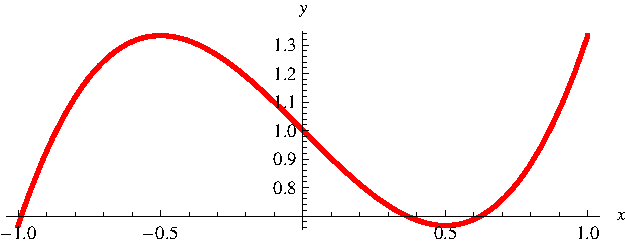
\includegraphics[height=2.8cm]{precalculus/pictures/01-01-inc-dec-a.pdf}%
%}%
%\only<handout:0| 3>{%
%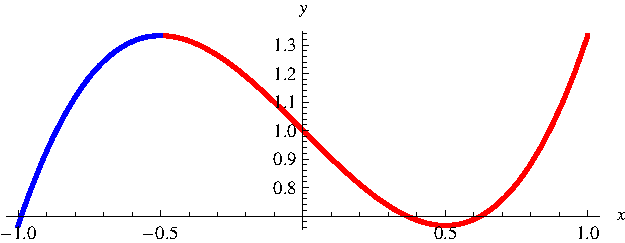
\includegraphics[height=2.8cm]{precalculus/pictures/01-01-inc-dec-b.pdf}%
%}%
%\only<handout:0| 4>{%
%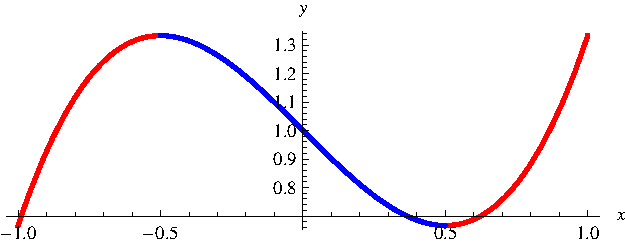
\includegraphics[height=2.8cm]{precalculus/pictures/01-01-inc-dec-c.pdf}%
%}%
%\only<handout:0| 5->{%
%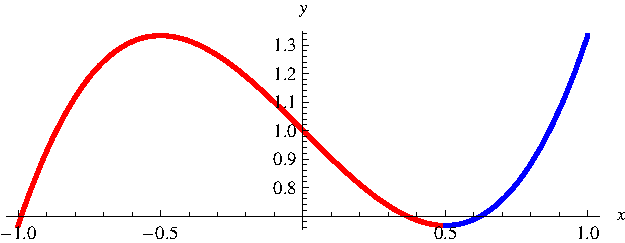
\includegraphics[height=2.8cm]{precalculus/pictures/01-01-inc-dec-d.pdf}%
%}%
\column{.4\textwidth}
\begin{itemize}
\item<3-| alert@3> \only<3>{\color{blue}} $f$ is increasing on $[-1, -\frac{1}{2}]$.
\item<4-| alert@4> \only<4>{\color{blue}} $f$ is decreasing on $[-\frac{1}{2}, \frac{1}{2}]$.
\item<5-| alert@5> \only<5>{\color{blue}} $f$ is increasing on $[\frac{1}{2}, 1]$.
\end{itemize}
\end{columns}
\end{example}
}
\end{frame}
% end module increasing-decreasing


}% end lecture

\lect{\semester}{Lecture  5}{5}{
%DesiredLectureName: Functions
\fcLicense
\section{A Catalog of Essential Functions}
\subsection{Linear Functions}
% begin module linear-functions
\begin{frame}
\frametitle{Linear Functions}
\begin{definition}[Linear Function]
A linear function is a function the graph of which is a line.  We can write any linear function in slope-intercept form:
\[
f(x) = mx + b.
\]
$m$ is called the slope, and $b$ is called the $y$-intercept.
\end{definition}
\begin{columns}
\column{0.5\textwidth}

\uncover<2->{
\psset{xunit=0.6cm, yunit=0.6cm}
\begin{pspicture}(-0.5,-0.5)(3.2,3)%
\tiny%
\fcAxesStandard{-0.5}{-0.5}{3}{2.8}%
\psline[linecolor=\fcColorGraph](-0.5, 0.5)(3,2.5)%
\fcLabels{3}{2.8}%
\end{pspicture}
\begin{itemize}
\item Any non-vertical line arises as the graph of a linear function.

\end{itemize}
}
\column{0.5\textwidth}
\uncover<3->{
\psset{xunit=0.6cm, yunit=0.6cm}
\begin{pspicture}(-0.5,-0.5)(3.2,3)%
\tiny%
\fcAxesStandard{-0.5}{-0.5}{3}{2.8}%
\psline[linecolor=\fcColorGraph](1.5, -0.5)(1.5,3)%
\fcLabels{3}{2.8}%
\end{pspicture}
\begin{itemize}
\item Vertical lines fail the vertical line test and therefore are not graphs of a function of $x$. 
\end{itemize}
}
\end{columns}
\end{frame}


% end module linear-functions

%\begin{frame}
\begin{columns}[c]
\column{.5\textwidth}

\psset{xunit=0.7cm, yunit=0.7cm}
\begin{pspicture}(-2.6, -2.5)(4.1,2.6)
\psframe*[linecolor=white](-2.6,-2.5)(4.1,2.6)
\tiny
\fcAxesStandard{-2.6}{-2.5}{5}{2.6}
\fcLabelXOne
\uncover<2>{
\psline[linecolor=red](-2.5, -1.5)(1.5, 2.5)
}
\uncover<3->{
\psline[linecolor=blue](-2.5, -1.5)(1.5, 2.5)
}
\uncover<2->{
\rput[l](1.5, 2){$y=x+1$}
}
\uncover<5->{
\fcFullDot{0}{1}
\rput[r](-0.1, 1){\alert<5>{$(0,1)$}}
}

\uncover<3>{
\psline[linecolor=red](-2.5, 1.25)(5, -2.5)
}
\uncover<4->{
\psline[linecolor=blue](-2.5, 1.25)(5, -2.5)
}
\uncover<3->{
\rput[r](3.3, -2){$y=-0.5x$}
}
\uncover<6->{
\fcFullDot{0}{0}
\rput[lb](0.1, 0.1){\alert<6>{$(0,0)$}}
}

\uncover<4>{
\psline[linecolor=red](-2.5,-1)(5, -1)
}
\uncover<5->{
\psline[linecolor=blue](-2.5, -1)(5, -1)
}
\uncover<4->{
\rput[t](4, -1.1){$y=-1$}
}
\uncover<7->{
\fcFullDot{0}{-1}
\rput[lt](0.1, -1.1){\alert<7>{$(0,-1)$}}
}
\end{pspicture}
%\ \only<handout:0| -2>{%
%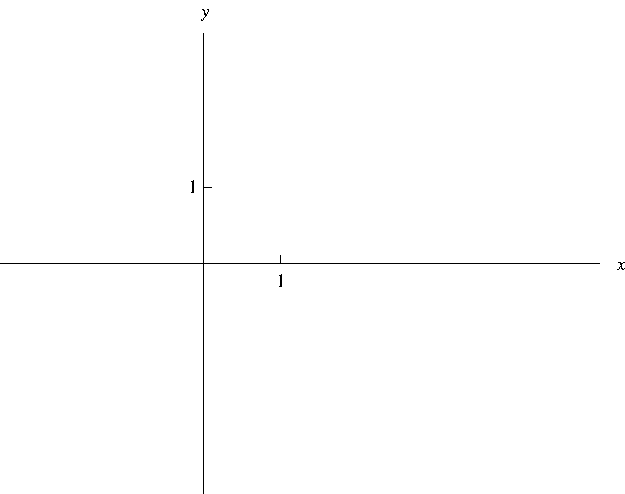
\includegraphics[height=4.5cm]{precalculus/pictures/01-02-linesa.pdf}%
%}%
%\only<handout:0| 3>{%
%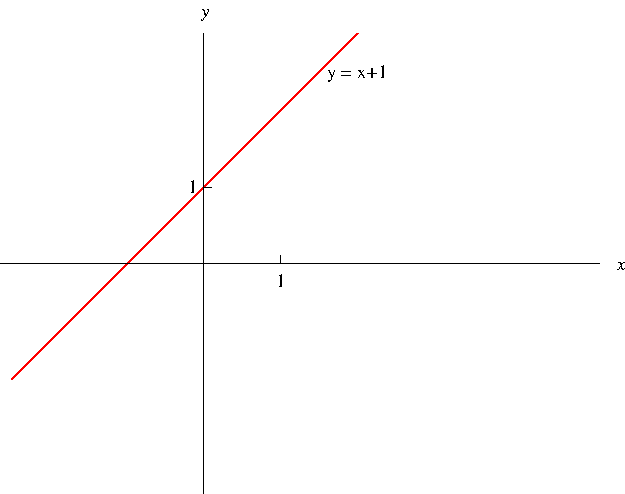
\includegraphics[height=4.5cm]{precalculus/pictures/01-02-linesb.pdf}%
%}%
%\only<handout:0| 4>{%
%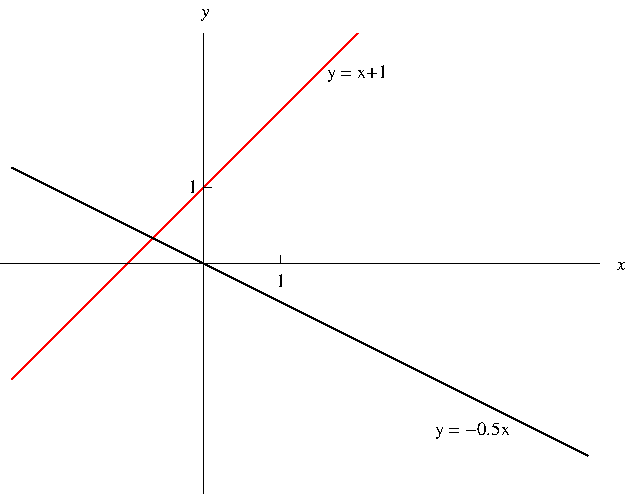
\includegraphics[height=4.5cm]{precalculus/pictures/01-02-linesc.pdf}%
%}%
%\only<handout:0| 5>{%
%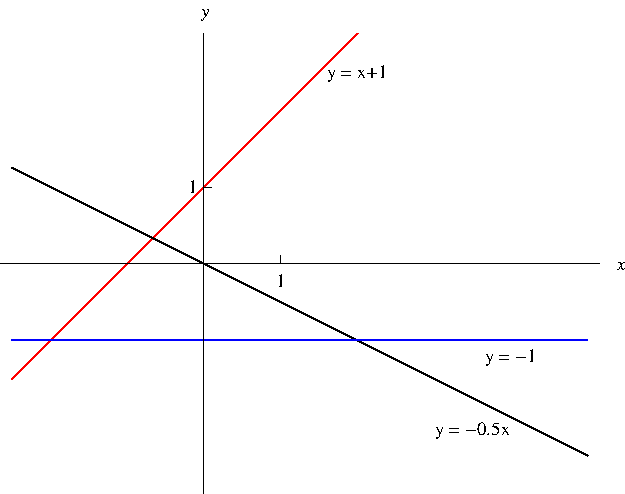
\includegraphics[height=4.5cm]{precalculus/pictures/01-02-linesd.pdf}%
%}%
%\only<handout:0| 6>{%
%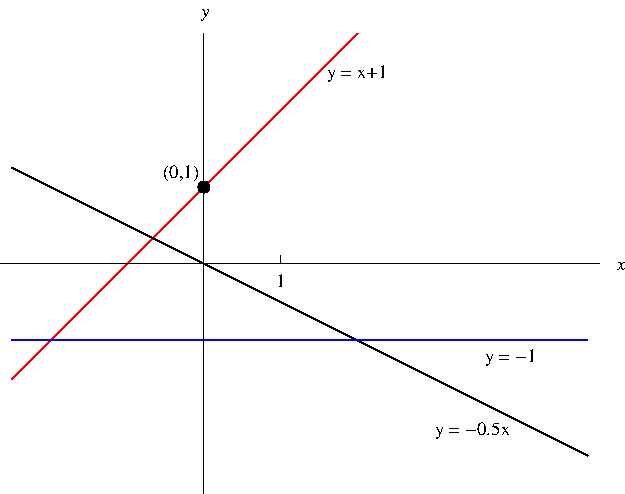
\includegraphics[height=4.5cm]{precalculus/pictures/01-02-linese.pdf}%
%}%
%\only<handout:0| 7>{%
%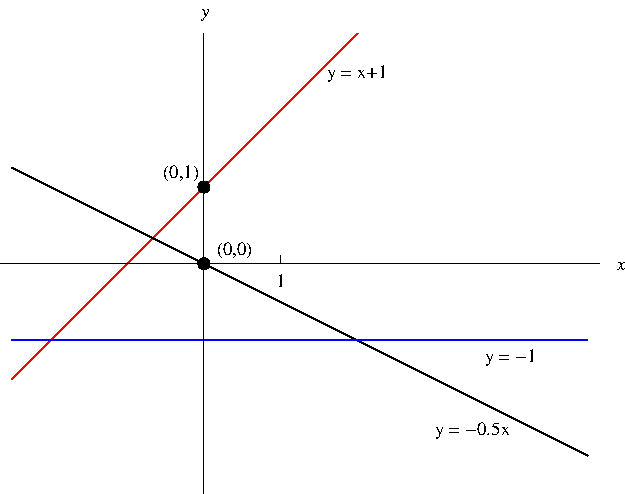
\includegraphics[height=4.5cm]{precalculus/pictures/01-02-linesf.pdf}%
%}%
%\only<8>{%
%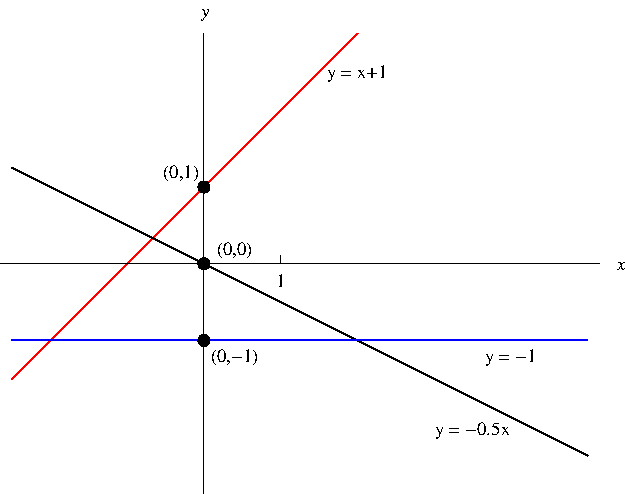
\includegraphics[height=4.5cm]{precalculus/pictures/01-02-linesg.pdf}%
%}%
\column[t]{.55\textwidth}
\begin{tabular}{|c|c|c|}
\hline
$f(x)$ & Direction & $y$-intercept \\
\hline
\uncover<1->{\alertNoH{ 2}{$x + \alertNoH{ 5}{1}$}} &
\uncover<2->{\alertNoH{ 2}{$\nearrow$}} &
\uncover<5->{\alertNoH{ 5}{1}} \\
\uncover<1->{\alertNoH{ 3}{$-0.5x \uncover<6>{\alertNoH{ 6}{+ 0}}$}} &
\uncover<3->{\alertNoH{ 3}{$\searrow$}} &
\uncover<6->{\alertNoH{ 6}{0}} \\
\uncover<1->{\alertNoH{ 4,7}{$-1$}} &
\uncover<4->{\alertNoH{ 4}{$\rightarrow$}} &
\uncover<7->{\alertNoH{ 7}{-1}} \\
\hline
\end{tabular}
\end{columns}

\begin{itemize}
\item<2->  $m > 0$ means the graph of $f$ points up ($\nearrow$).
\item<3->  $m < 0$ means the graph of $f$ points down ($\searrow$).
\item<4->  $m = 0$ means the graph of $f$ is horizontal ($\rightarrow$).
\item<5->  $b$ tells us the height of the point where the graph hits the $y$-axis.
\end{itemize}
\end{frame}
\subsection{Polynomials}
% begin module polynomials
\begin{frame}
\frametitle{Polynomials}
\begin{definition}[Polynomial Function]
A polynomial function is a function $f$ of the form
\[
f(x) = a_0 + a_1x + a_2x^2 + \cdots + a_{n - 1}x^{n-1} + a_nx^n ,
\]
where $n$ is a non-negative integer and $a_0, \ldots , a_n$ are real numbers, called the coefficients.

If the leading coefficient $a_n \neq 0$, then we say the degree of $f$ is $n$.
\end{definition}
\uncover<2->{
\[
\begin{array}{|c|c|c|c|c|c|}
\hline
f(x) &%
\alert<handout:0| 3-4,13-14,23-26,35-36>{\text{Polynomial?}} &%
\alert<handout:0| 5-6,15-16,27-28>{\text{Degree}} &%
\alert<handout:0| 7-8,17-18,29-30>{a_0} &%
\alert<handout:0| 9-10,19-20,31,32>{a_1} &%
\alert<handout:0| 11-12,21-22,33-34>{a_2} \\
\hline
\alert<handout:0| 3-12>{x^4-x+1} &%
\uncover<4->{\alert<handout:0| 4>{\text{Yes}}}&%
\uncover<6->{\alert<handout:0| 6>{4}}&%
\uncover<8->{\alert<handout:0| 8>{1}}&%
\uncover<10->{\alert<handout:0| 10>{-1}}&%
\uncover<12->{\alert<handout:0| 12>{0}}\\%
\alert<handout:0| 13-22>{6} &%
\uncover<14->{\alert<handout:0| 14>{\text{Yes}}}&%
\uncover<16->{\alert<handout:0| 16>{0}}&%
\uncover<18->{\alert<handout:0| 18>{6}}&%
\uncover<20->{\alert<handout:0| 20>{0}}&%
\uncover<22->{\alert<handout:0| 22>{0}}\\%
\alert<handout:0| 23>{3x^2 - \frac{1}{2}x + \alert<handout:0| 24>{\sqrt{x}}} &%
\uncover<24->{\alert<handout:0| 24>{\text{No}}}&%
&%
&%
&\\
\alert<handout:0| 25-34>{3x^2 - \frac{1}{2}x + \sqrt{2}} &%
\uncover<26->{\alert<handout:0| 26>{\text{Yes}}}&%
\uncover<28->{\alert<handout:0| 28>{2}}&%
\uncover<30->{\alert<handout:0| 30>{\sqrt{2}}}&%
\uncover<32->{\alert<handout:0| 32>{-\frac{1}{2}}}&%
\uncover<34->{\alert<handout:0| 34>{3}}\\%
\alert<handout:0| 35>{3x^2 - \frac{1}{2\alert<handout:0| 36>{x}} + \sqrt{2}} &%
\uncover<36->{\alert<handout:0| 36>{\text{No}}}&%
&%
&%
&\\
\hline
\end{array}
\]
}
\end{frame}


\begin{frame}
\begin{itemize}
\item<1->  Linear functions are polynomials.
\item<2->  So are quadratic functions.  Their graphs are parabolas.
\item<3->  And there are many more.
\end{itemize}
\only<handout:1| 1>{%
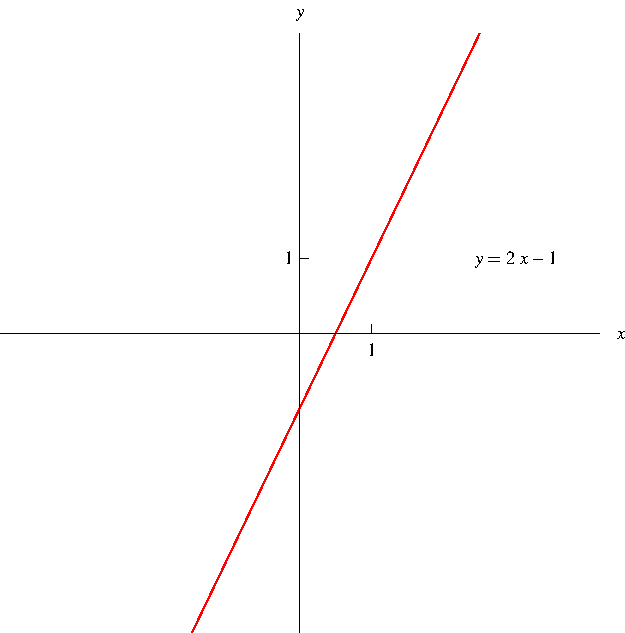
\includegraphics[height=6cm]{precalculus/pictures/01-02-line.pdf}%

Linear
}%
\only<handout:2| 2>{%
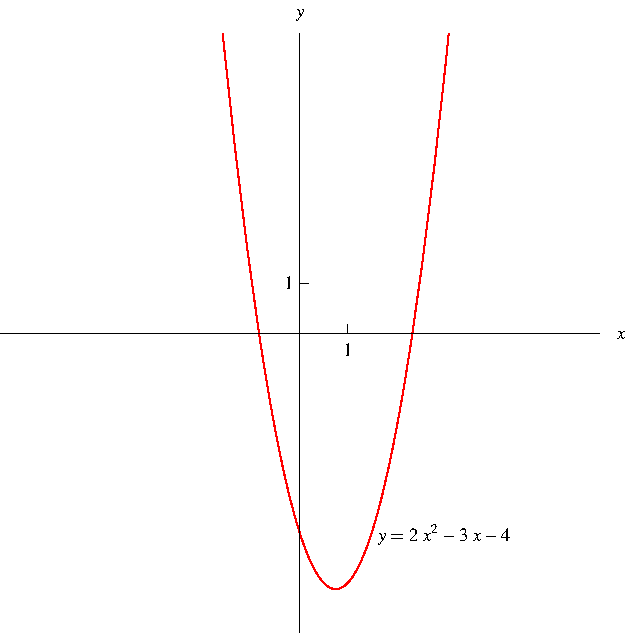
\includegraphics[height=6cm]{precalculus/pictures/01-02-parabola.pdf}%

Quadratic
}%
\only<handout:3| 3>{%
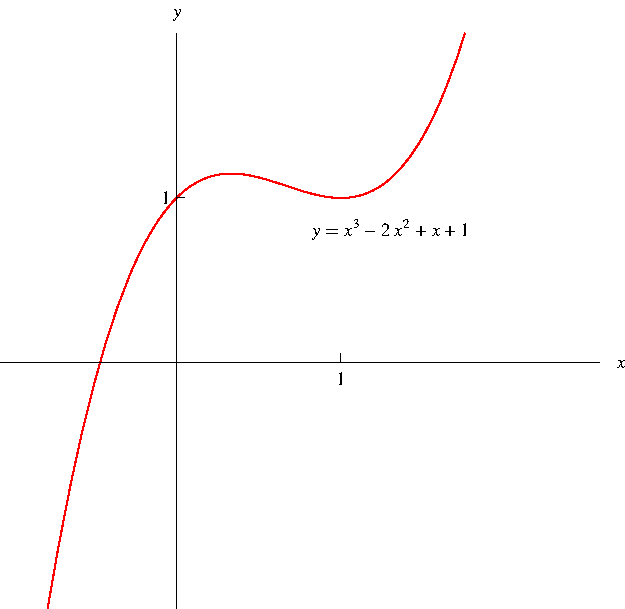
\includegraphics[height=6cm]{precalculus/pictures/01-02-polya.pdf}%

Cubic
}%
\only<handout:4| 4>{%
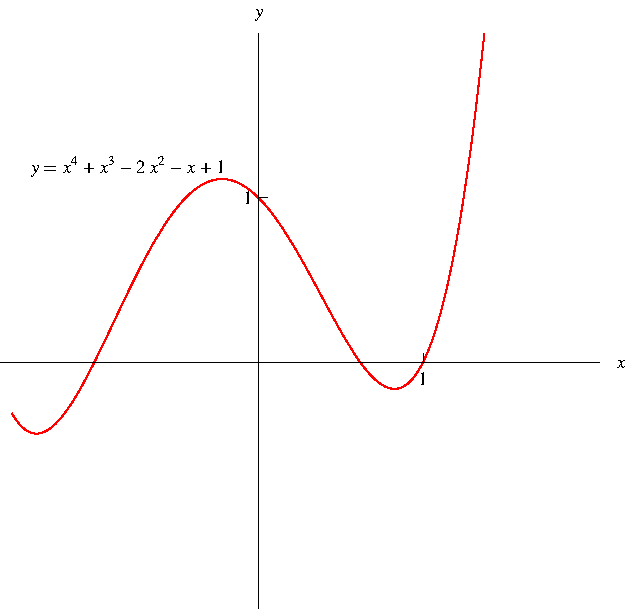
\includegraphics[height=6cm]{precalculus/pictures/01-02-polyb.pdf}%

Quartic
}%
\only<handout:5| 5>{%
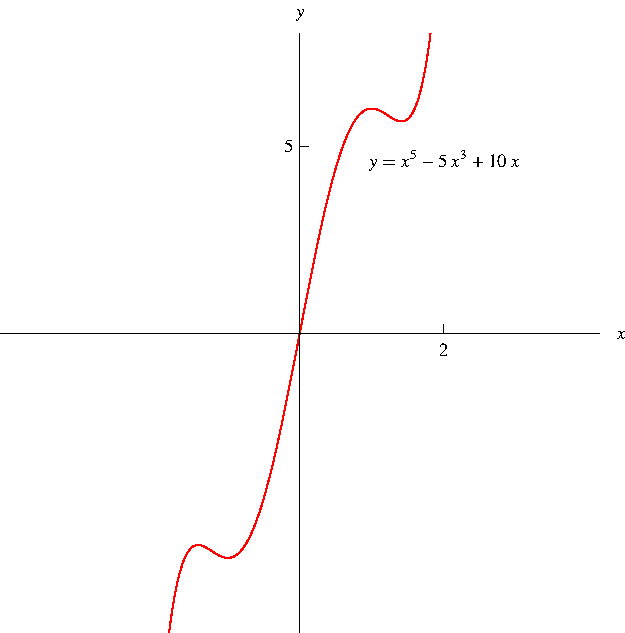
\includegraphics[height=6cm]{precalculus/pictures/01-02-polyc.pdf}%

Quintic
}
\end{frame}
% end module polynomials

\subsection{Power Functions}
%Old Version from Greg. Greg, this slide is changed substantially, please take a look.
%% begin module power-functions-def
%\begin{frame}
%\frametitle{Power Functions}
%\begin{definition}[Power Function]
%A power function is a function of the form
%\[
%f(x) = x^a,
%\]
%where $a$ is a fixed real number.
%\end{definition}
%\uncover<2->{
%If $a$ is a positive integer like $1, 2, 3, \ldots$ then $x^a$ is a polynomial.

%\only<handout:-2| -2>{%
%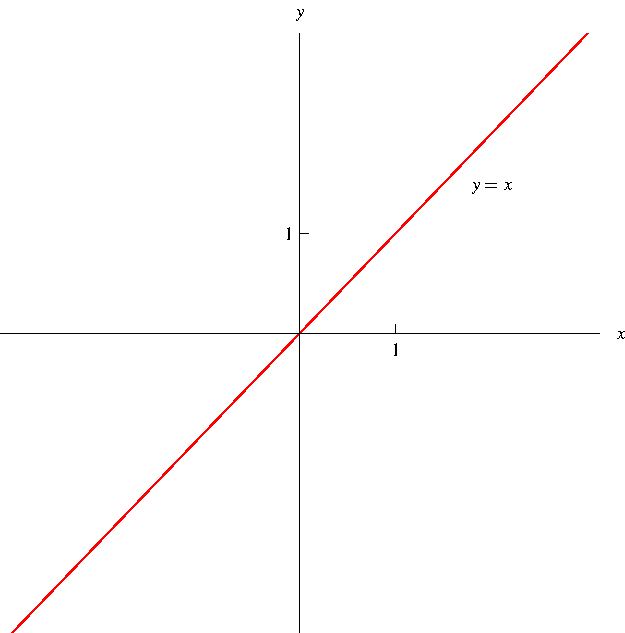
\includegraphics[height=4cm]{precalculus/pictures/01-02-x.pdf}%
%}%
%\only<handout:3| 3>{%
%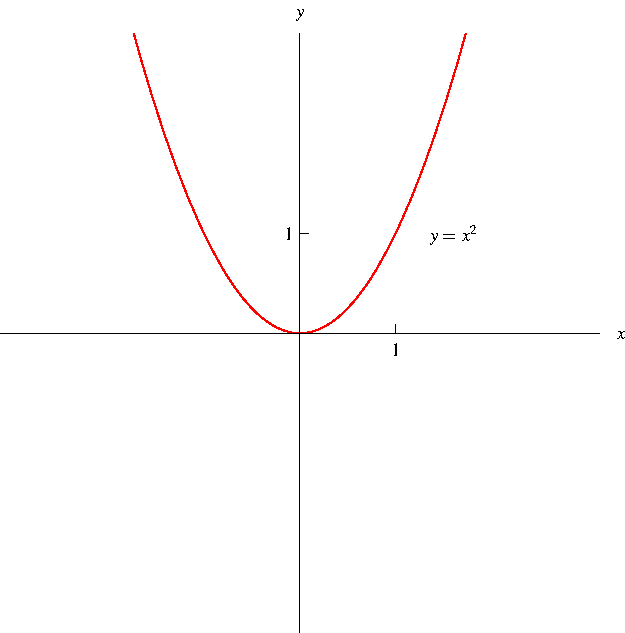
\includegraphics[height=4cm]{precalculus/pictures/01-02-xsquared.pdf}%
%}%
%\only<handout:4| 4>{%
%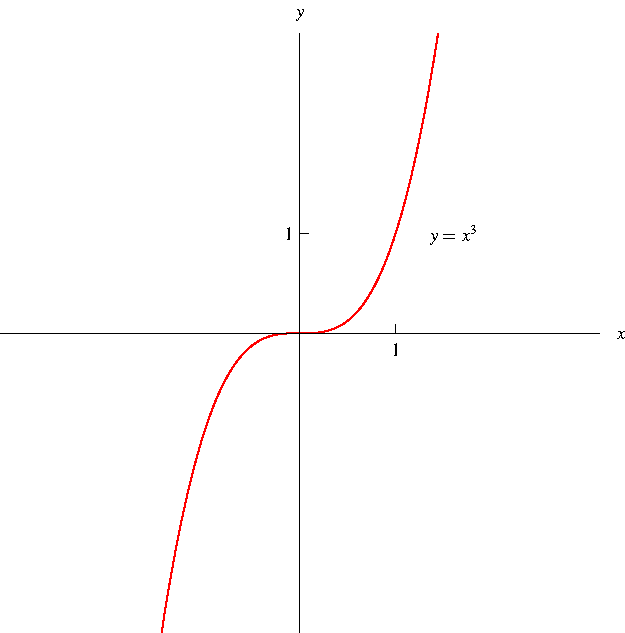
\includegraphics[height=4cm]{precalculus/pictures/01-02-xcubed.pdf}%
%}%
%\only<handout:5| 5>{%
%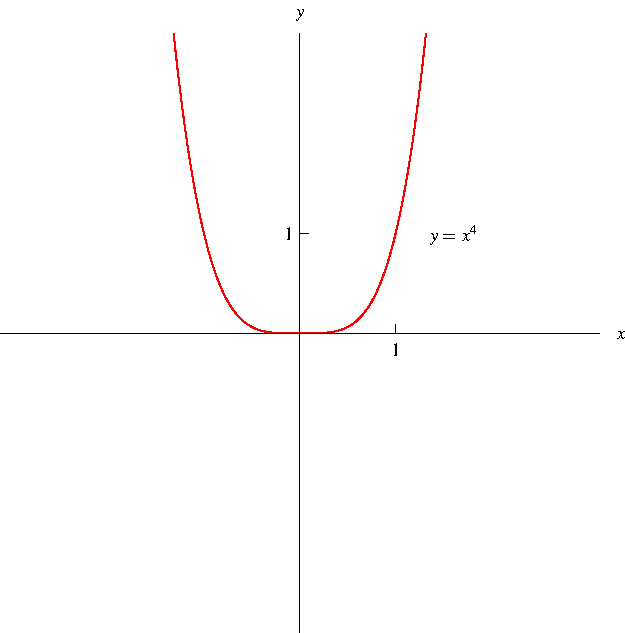
\includegraphics[height=4cm]{precalculus/pictures/01-02-xfourth.pdf}%
%}%
%\only<handout:6| 6>{%
%\includegraphics[height=4cm]{precalculus/pictures/01-02-xfifth.pdf}
%}%
%}%
%\end{frame}
%% end module power-functions-def

% begin module power-functions-def
\begin{frame}[t]
\frametitle{Power Functions}
\begin{definition}[Power Function]
Let $x>0$, $a$ - arbitrary real number. The power function is defined as
\[
f(x) \uncover<4->{\alertNoH{ 4}{=e^{a\ln x} } }= \alertNoH{2}{x}^{\alertNoH{3}{a}} \quad .
\]
\uncover<2->{$x$ = \alertNoH{2}{base}. } \uncover<3->{$a$ = \alertNoH{3}{exponent} or \alertNoH{3}{power}. }
\uncover<4->{\alertNoH{ 4}{First equality = one of ways to define for non-integer $a$ (we study $\ln x$, $e^x$ later). } }
\end{definition}
\begin{tabular}{@{}l}
\uncover<5->{
If $a$ - positive integer ($1, 2, 3, \ldots$) \\
then $x^a$ = polynomial function.
}\\
\uncover<5->{
$x^{n}    =\underbrace{x\dots x }_{n~\mathrm{times}}$ when $n$-integer. \\

$\begin{array}{rcl}
\alertNoH{12}{(x^{a})^b}&=&\fcAnswer{13}{x^{ab}}  \\
\alertNoH{14}{(xy)^b}   &=&\fcAnswer{15}{ x^by^b}\\
\alertNoH{16}{x^{a+b}}  &=&\fcAnswer{17}{x^ax^b } \\
\alertNoH{18}{x^{-a}}   &=&\fcAnswer{19}{\frac{1}{x^a}}
\end{array}
$\\
~\\~\\~\\~\\~\\~\\~\\
}
\end{tabular}
\uncover<6->{
\psset{xunit=0.38cm,yunit=0.38cm}
\begin{pspicture}(-5,-5)(5.4,5.2)
\psaxes[labels=none]{<->}(0,0)(-5,-5)(5,5)
\tiny
\rput[r](0,5){\tiny{$y$}}
\rput[l](5,0){\tiny{$x$}}
\only<handout:1|7>{
\psplot[linecolor=red]{-5}{5}{ x 1 exp }
\rput( 3, 1){$y=x^{\phantom{1}}$}
} %only
\only<handout:2|8>{
\psplot[linecolor=red]{-2.23}{2.23}{ x 2 exp }
\rput( 3, 1){$y=x^2$}
}
\only<handout:3|9>{
\psplot[linecolor=red]{-1.7}{1.7}{ x 3 exp }
\rput( 3, 1){$y=x^3$}
}
\only<handout:4|10>{
\psplot[linecolor=red]{-1.49}{1.49}{ x 4 exp }
\rput( 3, 1){$y=x^4$}
}
\only<handout:5|11->{
\psplot[linecolor=red]{-1.37}{1.37}{ x 5 exp }
\rput( 3, 1){$y=x^5$}
}
\end{pspicture}
\uncover<handout:5|11->{}
%\only<handout:-2| -2>{%
%\includegraphics[height=4cm]{precalculus/pictures/01-02-x.pdf}%
%}%
%\only<handout:3| 3>{%
%\includegraphics[height=4cm]{precalculus/pictures/01-02-xsquared.pdf}%
%}%
%\only<handout:4| 4>{%
%\includegraphics[height=4cm]{precalculus/pictures/01-02-xcubed.pdf}%
%}%
%\only<handout:5| 5>{%
%\includegraphics[height=4cm]{precalculus/pictures/01-02-xfourth.pdf}%
%}%
%\only<handout:6| 6>{%
%\includegraphics[height=4cm]{precalculus/pictures/01-02-xfifth.pdf}
%}%
}
\end{frame}
% end module power-functions-def

%Old Version from Greg. Greg, this slide is changed substantially, please take a look.
% begin module root-functions
%\begin{frame}
%\begin{itemize}
%\item<1->  If $n$ is a positive integer, the function $f(x) = x^{\frac{1}{n}} = \sqrt[n]{x}$ is called a root function.
%\item<2->  When $n = 2$, it is the square root function $f(x) = \sqrt{x}$.
%\item<3->  The square root is not defined for negative numbers, so its domain is $[0, \infty)$.
%\item<4->  Its graph is the top half of the parabola $x = y^2$.
%\item<5->  The graph of the cube root function $f(x) = \sqrt[3]{x}$ is similar to that of the square root, but it is defined everywhere.
%\end{itemize}
%\begin{tabular}{cc}
%\uncover<2->{%
%\includegraphics[height=3.5cm]{precalculus/pictures/01-02-sqrtx.pdf}%
%}%
%&%
%\uncover<5->{%
%\includegraphics[height=3.5cm]{precalculus/pictures/cube-root.pdf}%
%}%
%\end{tabular}
%\end{frame}
% end module root-functions

% begin module root-functions
\begin{frame}
\begin{itemize}
\item<1->  $n$ - positive integer, $f(x) = x^{\frac{1}{n}} = \sqrt[n]{x}$ = the $n^{th}$ root function. $\sqrt[n]{x}\geq 0$ for $x\geq 0$. 
\item<2->  For $n = 2$, we get the square root $\sqrt{x}$; for $n=3$ we get the cube root $\sqrt[3]{x}$, and so on. 
\item<3-> Let $x>0$. For $n=2m+1$-odd, we can extend the definition of $n^{th}$ root to negative numbers by $ \sqrt[2m+1]{-x}:= -\sqrt[2m+1]{x}$. 
\item<4-> In this course, even roots of negative numbers are not defined.
\item<5-> The graph of $\sqrt{x}$ is the top half of the parabola $x = y^2$. \uncover<6->{Similarly for $y=\sqrt[2m]{x}$, we graph top of $x=y^{2m}$.}
\item<7->  The graph of the cube root $f(x) = \sqrt[3]{x}$ is the graph of the polynomial $x=y^3$. \uncover<8->{Similarly for $y=\sqrt[2m+1]{x}$, we graph $x=y^{2m+1}$}.
\end{itemize}
\begin{tabular}{cc}
\uncover<5->{%
\psset{xunit=0.6cm,yunit=0.6cm}
\tiny
\begin{pspicture}(-3,-2)(3,2)
\psaxes[labels=none]{<->}(0,0)(-3,-2)(3,2)
\rput[r](0,2){{$y$}}
\rput[l](3,0){{$x$}}
\uncover<5>{
\psplot[linecolor=red]{0}{3}{ x 0.5 exp }
\rput( 3, 0.5){$y=\sqrt{x}$}
}
\uncover<6->{
\psplot[linecolor=red, plotpoints=300]{0}{3}{ x 0.25 exp }
\rput( 3, 0.5){$y=\sqrt[4]{x}$}
}
\end{pspicture}
%\uncover<2->{%
%\includegraphics[height=3.5cm]{precalculus/pictures/01-02-sqrtx.pdf}%
%}%
}%
&%
\uncover<7->{%
\psset{xunit=0.6cm,yunit=0.6cm}
\tiny
\begin{pspicture}(-3,-2)(3,2)
\psaxes[labels=none]{<->}(0,0)(-3,-2)(3,2)
\rput[r](0,2){\tiny{$y$}}
\rput[l](3,0){\tiny{$x$}}
\uncover<7>{
\psplot[linecolor=red, plotpoints=300]{-3}{0}{ x -1 mul 0.3333 exp -1 mul}
\psplot[linecolor=red, plotpoints=300]{0}{3}{ x         0.3333 exp }
\rput( 3, 0.5){$y=\sqrt[3]{x}$}
}
\uncover<8->{
\psplot[linecolor=red]{-3}{0}{ x -1 mul 0.2 exp -1 mul}
\psplot[linecolor=red]{0}{3}{ x         0.2 exp }
\rput( 3, 0.5){$y=\sqrt[5]{x}$}
}
\end{pspicture}
%\uncover<5->{%
%\includegraphics[height=3.5cm]{precalculus/pictures/cube-root.pdf}%
%}%
}%
\end{tabular}
\end{frame}
% end module root-functions
% begin module reciprocal-function
\begin{frame}
$f(x) = x^{-1} = \frac{1}{x}$ is called the reciprocal function.  Its graph has equation $y = \frac{1}{x}$, or $xy = 1$, and is an hyperbola with the coordinate axes as its asymptotes.
%\begin{center}%center does not work with well with pstricks and pgflayout.
\hfil\hfil\psset{xunit=0.6cm, yunit=0.6cm}
\begin{pspicture}(-5, -5)(5,5)
\psframe*[linecolor=white](-5,-5)(5,5)
\psaxes[ticks=none, labels=none]{<->}(0,0)(-5,-5)(5,5)\tiny
%Function formula: (1)/(x)
\rput(1,3){$y=\frac 1 x$}
\psplot[linecolor=red, plotpoints=1000]{0.2}{5}{1 x div } %Function formula: (1)/(x)
\rput(1,3){$y=\frac 1 x$}
\psplot[linecolor=red, plotpoints=1000]{-5}{-0.2}{1 x div }
\fcLabels{4.5}{4.5}
\end{pspicture}
%\includegraphics[height=5cm]{precalculus/pictures/reciprocal-function.pdf}%
%\end{center}
\end{frame}
% end module reciprocal-function

\subsection{Rational Functions}
% begin module rational-functions
\begin{frame}
\frametitle{Rational Functions}
\begin{definition}[Rational Function]
A rational function is a quotient of two polynomials; that is, a function of the form
\[
f(x) = \frac{g(x)}{h(x)},
\]
where $g$ and $h$ are polynomials.
\end{definition}
\begin{columns}[c]
\column{.4\textwidth}
\uncover<2->{
\psset{xunit=0.4cm, yunit=0.4cm}
\begin{pspicture}(-5, -5)(5,5)
\psframe*[linecolor=white](-5,-5)(5,5)
\psaxes[ticks=none, labels=none]{<->}(0,0)(-4.5,-4.5)(4.5,4.5)\tiny
%Function formula: \frac{x}{(x)^{2}-1}
\rput(2.5,-3){$y=\frac{x}{x^{2}-1}$}
\psplot[linecolor=red, plotpoints=1000]{1.11727}{4.5}{x -1 x 2 exp add div } %Function formula: \frac{x}{(x)^{2}-1}
\psplot[linecolor=red, plotpoints=1000]{-0.895043}{0.895043}{x -1 x 2 exp add div } %Function formula: \frac{x}{(x)^{2}-1}
\psplot[linecolor=red, plotpoints=1000]{-4.5}{-1.11727}{x -1 x 2 exp add div }
\fcLabels{4.5}{4.5}
\end{pspicture}
%\includegraphics[height=4cm]{precalculus/pictures/01-02-rational.pdf}%
}
\column{.6\textwidth}
\uncover<2->{
\begin{example}[$x/(x^2-1)$]
The function
\[
f(x) = \frac{x}{x^2-1}
\]
is a rational function.
\end{example}
}
\end{columns}
\end{frame}
% end module rational-functions

\subsection{Algebraic Functions}
%Old Version from Greg. Greg, this slide is changed substantially, please take a look.
%% begin module algebraic-functions
%\begin{frame}
%\frametitle{Algebraic Functions}
%\begin{definition}[Algebraic Function]
%An algebraic function is a function that can be constructed using algebraic operations (such as addition, subtraction, multiplication, division, and taking roots) starting from polynomials.
%\end{definition}
%\uncover<2->{
%Algebraic functions can look pretty funny.
%\begin{tabular}{ccc}
%\includegraphics[height=3.8cm]{precalculus/pictures/01-02-algebraic1.pdf}&%
%\includegraphics[height=3.8cm]{precalculus/pictures/01-02-algebraic2.pdf}&%
%\includegraphics[height=3.8cm]{precalculus/pictures/01-02-algebraic3.pdf}%
%\end{tabular}
%}
%\end{frame}
%% end module algebraic-functions


% begin module algebraic-functions
\begin{frame}
\frametitle{Algebraic Functions}
\begin{definition}[Algebraic Function]
A function in $x$ that can be constructed using $x$, constants, and finitely many of the operations $+, -, *, /,$ and $\sqrt[n]{~}$ is an algebraic function.

\uncover<2->{{\footnotesize Outside of Calculus I: function $f(x)$ = algebraic if it satisfies a polynomial equation with polynomial coefficients, i.e., $a_0(x) +a_1(x)f(x)+\dots +a_n(x) \left(f(x)\right)^n=0$ for some polynomials  $a_i(x)$.}}
\end{definition}
\uncover<3->{
Examples.

\begin{tabular}{ccc}
\psset{xunit=0.3cm, yunit=0.3cm}
\begin{pspicture}(-5, -5)(5,5) 
\tiny\psframe*[linecolor=white](-5,-5)(5,5) 
\psaxes[ticks=none, labels=none]{<->}(0,0)(-4.5,-4.5)(4.5,4.5)\tiny
%Function formula: - ((- (x))^{5/3})- ((- (x))^{2/3}) 
\psplot[linecolor=red, plotpoints=1000]{-2}{-0.001}{x -1 mul 0.666667 exp -1 mul x -1 mul 1.66667 exp -1 mul add } %Function formula: (x)^{5/3}- ((x)^{2/3}) 
\rput[t](1,-5){$y=(x-1)\sqrt[3]{x^2}$} 
\psplot[linecolor=red, plotpoints=1000]{0.001}{3}{x 0.666667 exp -1 mul x 1.66667 exp add }
\psLabels{4.5}{4.5}
\end{pspicture} 
%\includegraphics[height=3.8cm]{precalculus/pictures/01-02-algebraic1.pdf}
&%
\psset{xunit=0.3cm, yunit=0.3cm}
\begin{pspicture}(-5, -5)(5,5) 
\tiny\psframe*[linecolor=white](-5,-5)(5,5) 
\psaxes[ticks=none, labels=none]{<->}(0,0)(-4.5,-4.5)(4.5,4.5)\tiny
\psplot[linecolor=red, plotpoints=1000]{1}{5}{-1 x 2 exp add 0.5 exp x 2 exp mul -0.2 mul -1 x 2 exp add 0.5 exp x mul 0.8 mul add } %Function formula: 4/5 ((x) (((x)^{2}-1)^{1/2}))-1/5 (((x)^{2}) (((x)^{2}-1)^{1/2})) 
\rput[t](1,-5){$y=\frac15(4x-x^2)\sqrt{x^2-1}$} 
\psplot[linecolor=red, plotpoints=1000]{-2}{-1}{-1 x 2 exp add 0.5 exp x 2 exp mul -0.2 mul -1 x 2 exp add 0.5 exp x mul 0.8 mul add }
\psLabels{4.5}{4.5}
\end{pspicture} 
%\includegraphics[height=3.8cm]{precalculus/pictures/01-02-algebraic2.pdf}
&%
\psset{xunit=0.3cm, yunit=0.3cm}
\begin{pspicture}(-5, -5)(5,5) 
\tiny\psframe*[linecolor=white](-5,-5)(5,5) 
\psaxes[ticks=none, labels=none]{<->}(0,0)(-4.5,-4.5)(4.5,4.5)\tiny
%Function formula: - ((4- ((x)^{2}))^{1/2})+(x) ((4- ((x)^{2}))^{1/2}) 
\rput[t](1,-5){$y=(x-1)\sqrt{4-x^2}$} 
\psplot[linecolor=red, plotpoints=1000]{-2}{2}{x 2 exp -1 mul 4 add 0.5 exp x mul x 2 exp -1 mul 4 add 0.5 exp -1 mul add }
\psLabels{4.5}{4.5}
\end{pspicture} 
%\includegraphics[height=3.8cm]{precalculus/pictures/01-02-algebraic3.pdf}
%
\end{tabular}
}
\end{frame}
% end module algebraic-functions

\subsection{Transcendental Functions}
% begin module transcendental-functions
\begin{frame}
\frametitle{Transcendental Functions}
Transcendental functions include many classes of functions.
\begin{itemize}
\item<2->  Trigonometric functions such as $\cos x, \sin x, \tan x,$ etc.
\item<3->  Exponential functions such as $2^x, \left( \frac{1}{2}\right)^x, 5^x, e^x$, etc.
\item<4->  The logarithm function $\ln x$.
\item<5->  And many more.
\item<6-> Outside of Calculus I: by definition, a function is transcendental if it is not algebraic, i.e., if it satisfies no polynomial equation with polynomial coefficients.
\end{itemize}
\end{frame}
% end module transcendental-functions 

\subsection{Miscellaneous}
% begin module greatest-integer-function
\begin{frame}
\begin{definition}[Greatest Integer Function]
The \emph{greatest integer function} $\lfloor x\rfloor$ is defined as the largest integer that is less than or equal to $x$.
\end{definition}
In computer science this function is called the \emph{floor} function.
\begin{columns}[c]
\column{.5\textwidth}
\psset{xunit=1cm, yunit=1cm}
\begin{pspicture}(-1.5, -1.5)(3.8,3.8)
\psaxes[labels=x, ticks=x]{<->}(0,0)(-1.5,-1.5)(3.8,3.8)
\psline(-0.1,1)(0.1,1)
\rput[b](-0.25, 1){$1$}
\psline[linecolor=red](-1,-1)(0,-1)
\psFullDot{-1}{-1}
\psHollowDot{0}{-1}

\psline[linecolor=red](0,0)(1,0)
\psFullDot{0}{0}
\psHollowDot{1}{0}

\psline[linecolor=red](1,1)(2,1)
\psFullDot{1}{1}
\psHollowDot{2}{1}

\psline[linecolor=red](2,2)(3,2)
\psFullDot{2}{2}
\psHollowDot{3}{2}

\psline[linecolor=red](3,3)(3.8,3)
\psFullDot{3}{3}
%\psHollowDot{4}{3}
\end{pspicture}
%\ \includegraphics[height=4.5cm]{continuity/pictures/02-05-ex2d.pdf}%

\column{.5\textwidth}
\begin{align*}
\uncover<2->{%
\alert<handout:0| 2-3>{%
\lfloor 
4 
\rfloor
}}%
& \uncover<2->{%
\alert<handout:0| 2-3>{%
 = \uncover<handout:0| 3->{%
 4%
}}}\\%
\uncover<2->{%
\alert<handout:0| 4-5>{%
\lfloor 
4.8%
\rfloor
}}%
& \uncover<2->{%
\alert<handout:0| 4-5>{%
 = \uncover<handout:0| 5->{%
 4%
}}}\\%
\uncover<2->{%
\alert<handout:0| 6-7>{%
\lfloor 
\pi%
\rfloor
}}%
& \uncover<2->{%
\alert<handout:0| 6-7>{%
 = \uncover<handout:0| 7->{%
 3%
}}}\\%
\uncover<2->{%
\alert<handout:0| 8-9>{%
\lfloor 
\sqrt{2}%
\rfloor
}}%
& \uncover<2->{%
\alert<handout:0| 8-9>{%
 = \uncover<handout:0| 9->{%
 1%
}}}\\%
\uncover<2->{%
\alert<handout:0| 10-11>{%
\left\lfloor 
-\frac{1}{2}%
\right\rfloor %
}}%
& \uncover<2->{%
\alert<handout:0| 10-11>{%
 = \uncover<handout:0| 11->{%
-1%
}}}\\%
\uncover<2->{%
\alert<handout:0| 12-13>{%
\left\lfloor 
-\pi%
\right\rfloor %
}}%
& \uncover<2->{%
\alert<handout:0| 12-13>{%
 = \uncover<handout:0| 13->{%
-4%
}}}%
\end{align*}
\end{columns}
\end{frame}
% end module greatest-integer-function

\section{New Functions from Old Functions}
% begin module combinations-functions
\begin{frame}
\frametitle{Combinations of Functions}
Two functions $f$ and $g$ can be combined to form new functions $f+g$, $f-g$, $fg$, and $f/g$.  The sum and difference functions are defined by the formulas
\[
(f+g)(x) = f(x) + g(x), \qquad (f-g)(x) = f(x)-g(x).
\]
If $A$ is the domain of $f$ and $B$ is the domain of $g$, then the domain of $f+g$ and $f-g$ is $A\cap B$, the intersection of $A$ and $B$.

The product and quotient functions are defined by the formulas
\[
(fg)(x) = f(x)g(x), \qquad \left( \frac{f}{g}\right)(x) = \frac{f(x)}{g(x)}.
\]
These functions also have the domain $A\cap B$, with one exception: in the quotient function, we aren't allowed to divide by 0, so we must exclude those values of $x$ that make $g(x) = 0$.  We write this domain as
\[
\{ x\in A\cap B | \ g(x) \neq 0\} .
\]
\end{frame}
% end module combinations-functions

% begin module composition-functions
\begin{frame}
\begin{definition}[Composition of $f$ and $g$]
If $f$ and $g$ are two functions, then the composition of $f$ and $g$ is written $f\circ g$ and is defined by the formula
\[
(f\circ g)(x) = f(g(x)).
\]
\end{definition}

Imagine $f$ and $g$ as machines taking some input and producing some output. Then $f\circ g$ corresponds to attaching both machines end-to-end so that the output of $g$ becomes the input of $f$.

\psset{xunit=0.75cm, yunit=0.75cm}
\begin{pspicture}(-4, -2.5)(13,2.5) 
\footnotesize
\rput[r] (-3.1, 0){$x$}
\psline[linewidth=3pt]{->}(-3,0)(-2.25,0)

\rput(0.25,0){
\psMachine{$g$}{blue}
}
\rput (4, 0){$g(x)$}
\psline[linewidth=3pt]{->}(2.75,0)(3.5,0)
\psline[linewidth=3pt]{->}(4.5,0)(5.25,0)
\rput(7.75,0){
\psMachine{$f$}{red}
}
\rput (11.75, 0){$f(g(x))$}
\psline[linewidth=3pt]{->}(10.25,0)(11,0)
\end{pspicture} 
%\includegraphics[height=2cm]{precalculus/pictures/01-03-machines.pdf}%

\uncover<2->{
The domain of $f\circ g$ is the set of all numbers $x$ in the domain of $g$ such that $g(x)$ is in the domain of $f$.  If the domain of $f$ is $A$ and the domain of $g$ is $B$, we write this as
\[
\{ x\in B |\ g(x) \in A\} .
\]
}
\end{frame}
% end module composition-functions
% begin module composition-example
\begin{frame}
\begin{example}
Find $\alertNoH{2}{f\circ g},\alertNoH{14}{g\circ f}, \alertNoH{27}{g\circ g}$ and their domains, where \alertNoH{10,16}{$\alertNoH{5}{ f(} \alertNoH{6}{ x} \alertNoH{5}{) =}\only<handout:0|5> {\color{red}} \sqrt{\only<handout:0|5>{\color{black}} \alertNoH{6}{x}}$} and \alertNoH{4,29}{$\alertNoH{17,30}{ g(}\alertNoH{18,31}{ x} \alertNoH{17,30}{) = }\only<handout:0|17,30>{\color{red}} \sqrt{3 - \only<handout:0|17,30>{ \color{black}} \alertNoH{18,31}{x} }$}.

$
\begin{array}{rclll}
\only<handout:1|1-26>{%
\uncover<2->{\alertNoH{3}{ (\alertNoH{2}{f\circ g})(x)}} &\uncover<3->{ \alertNoH{3}{ =}} & \uncover<3->{\alertNoH{3}{ f(\alertNoH{4}{g(x)})}} \uncover<4->{ =\only<handout:0|5>{\color{red}} f\left( \only<handout:0|5>{ \color{black}}   \alertNoH{4,6}{\sqrt{3 - x}} \only<handout:0|5>{\color{red}} \right)} \uncover<5->{ = \only<handout:0|5>{ \color{red}}  \alertNoH{7}{\sqrt{ \only<handout:0|5>{ \color{black}} \alertNoH{6}{\sqrt{3-x}}}}} \uncover<7->{  \alertNoH{7}{= \sqrt[4]{\alertNoH{7,9}{ 3-x} }}}\\
\uncover<8->{\text{Domain: }}\\
\uncover<9->{\alertNoH{9}{\alertNoH{10}{3}-x}&\alertNoH{9}{\geq} & \alertNoH{9}{0}} \\ 
\uncover<10->{\alertNoH{11}{-}x&\alertNoH{11}{\geq} & \alertNoH{10}{ \alertNoH{11}{-} 3}}\\
\uncover<11->{\alertNoH{13}{x}&\alertNoH{11,13}{\leq}&\alertNoH{13}{ 3} }\\
\uncover<12->{\alertNoH{12,13}{x} &\alertNoH{12,13}{\in}& \fcAnswer{13}{(-\infty , 3].}}\\
\uncover<14->{\alertNoH{15}{ (\alertNoH{14}{g\circ f})(x)}}& \uncover<15->{ \alertNoH{15}{=} } & \uncover<15->{ \alertNoH{15}{ g(\alertNoH{16}{ f(x)})}}
\uncover<16->{ = \alertNoH{17}{g(}\alertNoH{16,18}{\sqrt{x}}\alertNoH{17}{)}} \uncover<17->{ = \only<handout:0|17>{\color{red}}  \sqrt{\alertNoH{21}{ 3 - \only<handout:0|17>{ \color{black}} \alertNoH{18}{\sqrt{\alertNoH{20}{x}} }} }}\\
\uncover<19->{\text{Domain}:}\\
\uncover<20->{\alertNoH{20,26}{x}&\alertNoH{20,26}{\geq} & \alertNoH{20,26}{0} }\\
\uncover<21->{\alertNoH{21}{\alertNoH{22}{ 3} - \sqrt{x}}& \alertNoH{21}{ \geq } & \alertNoH{21}{ 0} }\\
\uncover<22->{ \alertNoH{23}{-} \sqrt{x} &\alertNoH{23}{\geq }& \alertNoH{22}{ \alertNoH{23}{-}3 }}\\
\uncover<23->{\sqrt{x}&\alertNoH{23}{ \leq} & 3} \\
\uncover<24->{\alertNoH{26}{ x}& \alertNoH{26}{ \alertNoH{0}{\leq}} &\alertNoH{26}{ 9}}\\
\uncover<25->{ \alertNoH{25,26}{x}&\alertNoH{25,26}{\in}& \fcAnswer{26}{[0,9]}} \\
}%only<handout:1|1->  
\only<handout:2|27->{%
\uncover<27->{\alertNoH{28}{ (\alertNoH{27}{g\circ g})(x)}} & \uncover<28->{ \alertNoH{28} {=} } & \uncover<28->{\alertNoH{28}{ g( \alertNoH{29 }{ g(x)})}} \uncover<29->{ = \only<handout:0|30>{\color{red}}  g \left( \only<handout:0|30>{ \color{black}} \alertNoH{29}{\sqrt{3 - x}}  \only<handout:0|30>{\color{red}} \right)}  \uncover<30->{ \only<handout:0|30>{\color{red}} = \sqrt{\alertNoH{36}{ 3 - \only<handout:0|30>{\color{black}}\alertNoH{31}{\sqrt{\alertNoH{33}{3-x} } }}}}\\
\uncover<32->{\text{Domain}:}\\
\uncover<33->{\alertNoH{33}{\alertNoH{34} {3}-x} & \alertNoH{33}{\geq} &\alertNoH{33}{ 0}}\\
\uncover<34->{\alertNoH{35}{-}x&\alertNoH{35}{\geq} & \alertNoH{34}{ \alertNoH{35}{ - } 3}}\\ 
\uncover<35->{\alertNoH{43}{x}&\alertNoH{35,43}{\leq} &\alertNoH{43}{ 3}}\\ 
\uncover<36->{\alertNoH{36}{\alertNoH{37}{3}-\sqrt{3-x}}&\alertNoH{36}{\geq }&\alertNoH{36}{ 0}} \\
\uncover<37->{\alertNoH{38}{-}\sqrt{3-x}&\alertNoH{38}{\geq}& \alertNoH{37}{\alertNoH{38}{-} 3}}\\
\uncover<38->{\sqrt{3-x}&\alertNoH{38}{\leq}& 3} \\
\uncover<39->{\alertNoH{40}{3}-x&\alertNoH{0}{\leq} &\alertNoH{40}{ 9}}\\
\uncover<40->{\alertNoH{41}{-}x&\alertNoH{41}{\leq}& \alertNoH{40}{6}}\\
\uncover<41->{\alertNoH{43}{x}&\alertNoH{41,43}{\geq}& \alertNoH{43}{ \alertNoH{41}{-}6} }\\  
\uncover<42->{\alertNoH{42,43}{x}&\alertNoH{42,43}{\in}& \fcAnswer{43}{[-6 , 3].}}
}%only<handout:2|>
\end{array}
$

%\column{.2\textwidth}
%\begin{eqnarray*}
%& & f\circ f  \\
%& & \uncover<2->{(f\circ f)(x)}\\
%& \uncover<3->{ = } & \uncover<3->{f(\alert<handout:0| 4>{f(x)})}\\
%& \uncover<4->{ = } & \uncover<4->{\alert<handout:0| 5>{f(}\alert<handout:0| 4-5>{\sqrt{x}}\alert<handout:0| 5>{)}}\\
%& \uncover<5->{ = } & \uncover<5->{\alert<handout:0| 5>{\sqrt{\sqrt{x}}}}\\
%& \uncover<6->{ = } & \uncover<6->{\alert<handout:0| 5>{\sqrt[4]{x}}}\\
%\end{eqnarray*}
\end{example}

\vskip 10cm
\end{frame}
% end module composition-example

\begin{frame}
\vskip -0.2cm
\begin{example}
Give simplified f-las for $f\circ g$, $f\circ f$, $g\circ f$, $g\circ g$. \alertNoH{2,3,4,5,21,22,31,32}{Find the implied domains.}
$
\begin{array}{@{}r@{}c@{}l@{}l|l}
\displaystyle \alertNoH{26}{ \alertNoH{8,27}{f(} \alertNoH{9,28}{x} \alertNoH{8,27}{)} }& \alertNoH{26}{=} &\displaystyle  \alertNoH{26}{ \only<handout:0|8,27>{\color{red}} \frac{2 \only<handout:0|8,27>{\color{black}} \alertNoH{9,28}{x} \only<handout:0|8,27>{\color{red}} -1}{\alertNoH{3,34}{\only<handout:0|8,27>{\color{black}}  \alertNoH{9,28}{x} \only<handout:0|8,27>{\color{red}} +2}}} \uncover<2->{&& \alertNoH{2,3}{x \neq}  \fcAnswer{3}{-2}}\\
\displaystyle \alertNoH{7}{ g(x)}& \alertNoH{7}{=} &\displaystyle \alertNoH{7}{ \frac{2x+ 3}{\alertNoH{5,24}{5x-7}}} \uncover<4->{&& \alertNoH{4,5,24}{x \neq}} \fcAnswer{5}{ \alertNoH{24}{\frac{7}{5}}}\\
\uncover<6->{% 
\displaystyle (f\circ g)(x)&\alertNoH{0}{=} &\displaystyle f(\alertNoH{7}{g(x)}) \uncover<7->{ = \only<handout:0|8>{\color{red}} f\left( \only<handout:0|8>{\color{black}} \alertNoH{7,9}{ \frac{2x+3}{ \alertNoH{24}{5x-7} }} \only<handout:0|8>{\color{red}}\right)\only<handout:0|8>{\color{black}}}
\uncover<8->{ = \only<handout:0|8>{\color{red}} \frac{ \alertNoH{10}{2} \only<handout:0|8>{\color{black}} \left( \alertNoH{9}{\frac{2x +3}{5x -7}} \right) \only<handout:0|8>{ \color{red}} -\alertNoH{11}{ 1} }{ \only<handout:0|8>{ \color{black}} \alertNoH{9}{\frac{2 x+3}{ 5x -7}} \only<handout:0|8>{\color{red}}+\alertNoH{12}{2 }}}
}%uncover<6-> 
\\
\uncover<10->{
&\alertNoH{0}{=}&\displaystyle \frac{ \frac{\alertNoH{10}{2} (2x+3)}{\alertNoH{13}{ 5x-7} }\alertNoH{14}{-} \alertNoH{11}{\frac{5x- 7}{ \alertNoH{13}{ 5x-7}}} }{\frac{2x+3}{ \alertNoH{13}{ 5x-7}}+ \alertNoH{12}{\frac{\alertNoH{15}{ 2( 5x-7) }}{\alertNoH{13}{ 5x-7}}}} \uncover<13->{= \frac{\frac{ \alertNoH{17}{ 4x} +\alertNoH{18}{6} \alertNoH{14 }{\alertNoH{17, 18}{-}(}\alertNoH{17}{5x}\alertNoH{18}{ - 7}\alertNoH{14}{)}}{\fcCancel{16}{ \alertNoH{13}{5 x-7} }}}{ \frac{\alertNoH{19}{2x} +\alertNoH{20}{3}+ (\alertNoH{15}{\alertNoH{19}{10x} \alertNoH{20}{ -14}}) }{\fcCancel{16}{ \alertNoH{13}{5x -7} }} }} \uncover<17->{= \frac{ \alertNoH{17}{-x} +\alertNoH{18}{ 13} }{\alertNoH{23}{ \alertNoH{19}{12x} \alertNoH{20}{-11}} } \uncover<21->{ && \alertNoH{21-24} {x\neq} \fcAnswer{22}{ \alertNoH{23}{ \frac{11}{12}} , \alertNoH{24}{\frac{7}{5}}}}}
}%uncover<10->
\\
\uncover<25->{
(f\circ f)(x)&\alertNoH{0}{=}& \displaystyle f(\alertNoH{26}{f(x)})\uncover<26->{ =\only<handout:0|27>{\color{red}} f\left(\only<handout:0|27>{\color{black}} \alertNoH{26,28}{ \frac{ 2x- 1}{\alertNoH{34}{x+2} }} \only<handout:0|27>{ \color{red}} \right) \only<handout:0|27>{\color{black}} } \uncover<27->{ = \alertNoH{29,30}{ \only<handout:0|27>{ \color{red}} \frac{  2  \only<handout:0|27>{ \color{black}} \left( \alertNoH{28}{\frac{ 2x- 1}{x+2}} \right)\only<handout:0|27>{\color{red}} -1 }{\only<handout:0|27>{\color{black}} \alertNoH{28}{\frac{ 2x- 1}{x+2}} \only<handout:0|27>{\color{red}}+2 }}
}}%uncover<25->
\\
\uncover<29->{ & \alertNoH{29,30}{=} &\displaystyle  \fcAnswer{30}{\frac{3 x-4}{ \alertNoH{33}{4 x+3} }} \uncover<31->{ && \alertNoH{31-34}{x\neq} \!\! \fcAnswer{32}{ \alertNoH{34}{-2}, \! \alertNoH{33}{ -\frac{3}{4}}} }
}%uncover<29->
 \\
\uncover<35->{ \alertNoH{35,36}{(g\circ f)(x)} &\alertNoH{35,36}{=}& \fcAnswer{36}{ \frac{7 x+4}{3 x-19}} && \alertNoH{35,36}{x\neq}  \fcAnswer{36}{ -2,\frac{19}{3}}} \\
\uncover<35->{\alertNoH{35,36}{ (g\circ g)(x)}&\alertNoH{35,36}{=} &\fcAnswer{36}{ \frac{19 x-15}{-25 x+64}} && \alertNoH{35,36}{ x \neq } \fcAnswer{36}{ \frac{7}{5},  \frac{64}{25} }}
\end{array}
$

\end{example}
\end{frame}
}

\lect{\semester}{Lecture 6}{6}{
\section{Composing Functions with Linear Transformations}
% begin module transformations-shifts
\begin{frame}
\frametitle{Transformations of Functions}
\begin{columns}[c]
\column{.5\textwidth}

\psset{xunit=1cm, yunit=1cm}
\begin{pspicture}(-0.5, -0.5)(4.7,4.7)%
\tiny%
\psframe*[linecolor=white](-5,-5)(5,5)%
\psaxes[ticks=none, labels=none]{<->}(0,0)(-0.5,-0.5)(5,4.5)%
\rput[t](5, -0.1){$x$}%
\rput[r](-0.1, 4.5){$y$}%
%\frac{1}{3} (3 x-6)^{3}-\frac{1}{3} (3 x-6)^{2}-\frac{1}{3} x+\frac{8}{3} 
\newcommand{\theFun}{3 x mul 6 sub dup dup mul mul 3 div 3 x mul 6 sub dup mul -3 div x -3 div 8 3 div add add add\space}%
\only<handout:0| -2>{%
\psplot[linecolor=red, plotpoints=1000]{1.65}{2.55}{\theFun}%
\rput[b] (2.55, 2.40654){\alert<-2>{$y=f(x)$}}%
}%
\only<handout:1| 3->{%
\psplot[linecolor=blue, plotpoints=1000]{1.65}{2.55}{\theFun}%
\rput[b] (2.55, 2.40654){$y=f(x)$}%
}%
\only<handout:0| 3>{%
\psplot[linecolor=red, plotpoints=1000]{1.65}{2.55}{\theFun 1.5 add }%
\rput[b](2.55, 3.90654){\alert<3>{$y=f(x)+c$}}%
}%
\only<handout:1| 4,5,22->{%
\psplot[linecolor=blue, plotpoints=1000]{1.65}{2.55}{\theFun 1.5 add }%
\rput[b](2.55, 3.90654){$y=f(x)+c$}%
}%
\only<handout:0| 4>{%
\psplot[linecolor=red, plotpoints=1000]{1.65}{2.55}{\theFun 1.5 sub}%
\rput[b](2.55, 0.906542){$y=f(x)-c$}%
}%
\only<handout:1| 5,22->{%
\psplot[linecolor=blue, plotpoints=1000]{1.65}{2.55}{\theFun 1.5 sub}%
\rput[b](2.55, 0.906542){$y=f(x)-c$}%
}%
\only<handout:0| 19>{%
\psplot[linecolor=red, plotpoints=1000]{3.15}{4.05}{1 dict begin /x x 1.5 sub def \theFun end}%
}%
\only<handout:1| 20,22->{%
\psplot[linecolor=blue, plotpoints=1000]{3.15}{4.05}{1 dict begin /x x 1.5 sub def \theFun end}%
\rput[b](4.05, 2.40654){$\alert<20>{y=f(x-c)}$}%
}%
\newcommand{\theAnimation}[6]{%
\uncover<handout:0|####1>{%
\fcXTickWithLabel{\curPt}{$x$}%
}%
\uncover<handout:0|####2>{%
\fcXTickWithLabel{\curPt 1.5 sub}{$x-c$}%
}%
\uncover<handout:0|####3>{%
\rput[l](! \curPt 1.5 sub 0.1 add 1 dict begin /x \curPt 1.5 sub def \theFun  end 2 div){$f(x-c)$}%
}%
\uncover<handout:0|####4>{%
\psline[linecolor=red, linewidth=2pt](! \curPt 1.5 sub 0)(! \curPt 1.5 sub 1 dict begin /x \curPt 1.5 sub def \theFun  end)%
}%
\uncover<handout:0|####5>{%
\rput[l](! \curPt 0.1 add 1 dict begin /x \curPt 1.5 sub def \theFun  end 2 div){$f(x-c)$}%
}%
\uncover<handout:0|####6>{%
\psline[linecolor=red, linewidth=2pt](! \curPt 0)(! \curPt 1 dict begin /x \curPt 1.5 sub def \theFun  end)%
}%
}%
\newcommand{\curPt}{3.3\space}%
\theAnimation{7-10}{8-10}{9-10}{9-19}{10}{10-19}%
\renewcommand{\curPt}{3.5\space}%
\theAnimation{11-14}{12-14}{13-14}{13-19}{14}{14-19}%
\renewcommand{\curPt}{3.8\space}%
\theAnimation{15-19}{16-19}{17-18}{17-19}{18}{18-19}%
%

\only<handout:0|21>{%
\psplot[linecolor=red, plotpoints=1000]{0.15}{1.05}{1 dict begin /x x 1.5 add def \theFun end}
\rput[b](1.05, 2.40654){\alert<6>{$y=f(x+c)$}}
}
\only<handout:1|22->{%
\psplot[linecolor=blue, plotpoints=1000]{0.15}{1.05}{1 dict begin /x x 1.5 add def \theFun end}
\rput[b](1.05, 2.40654){$y=f(x+c)$}
}
\end{pspicture}
%\ \only<handout:0| -2>{%
%\includegraphics[height=5cm]{precalculus/pictures/01-03-shifta.pdf}%
%}%
%\only<handout:0| 3>{%
%\includegraphics[height=5cm]{precalculus/pictures/01-03-shiftb.pdf}%
%}%
%\only<handout:0| 4>{%
%\includegraphics[height=5cm]{precalculus/pictures/01-03-shiftc.pdf}%
%}%
%\only<handout:0| 5>{%
%\includegraphics[height=5cm]{precalculus/pictures/01-03-shiftd.pdf}%
%}%
%\only<6>{%
%\includegraphics[height=5cm]{precalculus/pictures/01-03-shifte.pdf}%
%}%a
\column{.5\textwidth}
\begin{itemize}
\item What happens to the graph if we add/subtract a positive constant $c$ in the equation of a function $f$?
\item What happens if we add or subtract $c$ from $x$ before applying the function $f$?
\end{itemize}
\end{columns}

\uncover<2->{
\begin{tabular}{|l|l|}
\hline
\alertNoH{ 3}{$f(x)+c$} &%
\uncover<3->{\alertNoH{3,22}{Shift the graph of $f(x)$ $c$ units up.}} \\%
\alertNoH{ 4}{$f(x)-c$} &%
\uncover<4->{\alertNoH{4,22}{Shift the graph of $f(x)$ $c$ units down.}} \\%
\alertNoH{6}{$f(x-c)$} &%
\uncover<6->{\alertNoH{6,22}{Shift the graph of $f(x)$ \fcAnswerUncover{6}{20}{$c$ units right}.}} \\%
\alertNoH{21}{$f(x+c)$} &%
\uncover<21->{\alertNoH{21,22}{Shift the graph of $f(x)$ $c$ units left.}}\\%
\hline
\end{tabular}

}
\end{frame}
% end module transformations-shifts

% begin module transformations-shifts-example
\begin{frame}
\begin{example}
Relative to the graph of $f(x)=x^2$, draw a graph of $f(x) = x^2 + 6x + 10$. \alertNoH{8}{Assume the graph of $f(x)=x^2$ given.}
\begin{columns}[c]
\column{0.45\textwidth}

\psset{xunit=0.65cm, yunit=0.65cm}
\begin{pspicture}(-5.5, -0.6)(3.1,5.1)
\tiny
\fcAxesStandard{-5.5}{-0.6}{3.1}{5.1}
\rput[rt](-0.1,-0.1){$(0,0)$}
%Function formula: (-3+x)^{2}-9+6 (x)
\only<handout:0| 8>{
\rput[l](1.9,2.4){$\alertNoH{8}{y=x^2}$}
\psplot[linecolor=\fcColorGraph, plotpoints=1000]{-2.23607}{2.23607}{x 6 mul -9 x -3 add 2 exp add add } %Function formula: (x)^{2}+10+6 (x)
\fcFullDot{0}{0}
}
\only<handout:1| 9->{
\rput[l](1.9,2.4){\color{gray}$y=x^2$}
\psplot[linecolor=gray, plotpoints=1000]{-2.23607}{2.23607}{x 6 mul -9 x -3 add 2 exp add add } %Function formula: (x)^{2}+10+6 (x)
\fcFullDot[linecolor=gray]{0}{0}
}
\only<handout:1| 9>{
\rput[l](-1.1,2.4){$\alertNoH{9}{y=(x-(-3))^2}$}
\psplot[linecolor=\fcColorGraph, plotpoints=1000]{-5.23607}{2.23607 3 sub}{x -3 sub dup mul}
\fcFullDot{-3}{0}
\rput[rt](-3.1, -0.1){$(-3,0)$}
}
\only<handout:1| 10->{
\rput[l](-1.1,2.4){\color{gray}$y=(x-(-3))^2$}
\psplot[linecolor=gray, plotpoints=1000]{-5.23607}{2.23607 3 sub}{x -3 sub dup mul}
\rput[rt](-3.1, -0.1){$(-3,0)$}
\fcFullDot[linecolor=gray]{-3}{0}
}
\only<handout:1| 10->{
\rput[rt](-3.1,0.9){$(-3,1)$}
\fcFullDot{-3}{1}
\rput[lb](-4.4,4.2){$\alertNoH{10}{y=x^{2}+6x+10}$}
\psplot[linecolor=red, plotpoints=1000]{-5}{-1}{x 6 mul 10 x 2 exp add add }
}
\only<handout:1| 9->{\psline[linecolor=blue, arrows=->](0,0)(-3,0)}
\only<handout:1| 10->{\psline[linecolor=blue, arrows=->](-3,0)(-3,1)}
\only<handout:1| 10->{\psline[linecolor=blue, arrows=->](0,0)(-3,1)}
\end{pspicture}

\column{.55\textwidth}
\uncover<2->{
Complete the square:
}
\[
\begin{array}{@{}rcl}
\uncover<3->{f(x)} & \uncover<3->{ = } & \uncover<3->{x^2 + 6x + 10} \\
& \uncover<4->{ = } & \uncover<4->{\left(\alertNoH{6}{ x^2 + 6x+ \fcAnswer{5}{ 9}} \right) + 10 - \fcAnswer{5}{ 9}} \\
& \uncover<6->{ = } & \uncover<6->{\alertNoH{6}{(x \alertNoH{7}{+} 3)^2} + 1} \\
& \uncover<7->{ = } & \uncover<7->{ \alertNoH{10}{ \alertNoH{9}{(x \alertNoH{7}{-} (\alertNoH{7}{-}3))^2} + 1}} \end{array}
\]
\end{columns}
\end{example}
\end{frame}
% end module transformations-shifts-example

% begin module transformations-magnifications
\begin{frame}
\begin{columns}[c]
\column{.5\textwidth}

\psset{xunit=0.7cm, yunit=0.7cm}
\begin{pspicture}(-4, -3.5)(4.5,5.2)
\tiny
\fcAxesStandard{-4}{-3.5}{4.5}{5.2}
%Function formula: 10/3+1/3 ((-3+3 (x))^{3})-1/3 ((-3+3 (x))^{2})-1/3 (x)
\only<handout:1| 1->{
\psplot[linecolor=red, plotpoints=1000]{1.65}{2.55}{x -0.333333 mul x 3 mul -6 add 2 exp -0.333333 mul x 3 mul -6 add 3 exp 0.333333 mul 2.66667 add add add }
\rput[b] (2.55, 2.40654){$y=f(x)$}
}
%\only<handout:0| 3->{
%\psplot[linecolor=blue, plotpoints=1000]{1.65}{2.55}{x -0.333333 mul x 3 mul %-6 add 2 exp -0.333333 mul x 3 mul -6 add 3 exp 0.333333 mul 2.66667 add add %add }
%\rput[b] (2.55, 2.40654){$y=f(x)$}
%}

\only<handout:0| 3>{
\psplot[linecolor=red, plotpoints=1000]{1.65}{2.55}{x -0.333333 mul x 3 mul -6 add 2 exp -0.333333 mul x 3 mul -6 add 3 exp 0.333333 mul 2.66667 add add add 2 mul}
\rput[b] (2.55, 4.80654){{$y=cf(x)$}}
}
\only<handout:1| 4->{
\psplot[linecolor=blue, plotpoints=1000]{1.65}{2.55}{x -0.333333 mul x 3 mul -6 add 2 exp -0.333333 mul x 3 mul -6 add 3 exp 0.333333 mul 2.66667 add add add 2 mul}
\rput[b] (2.55, 4.80654){$y=cf(x)$}
}

\only<handout:0| 4>{
\psplot[linecolor=red, plotpoints=1000]{1.65}{2.55}{x -0.333333 mul x 3 mul -6 add 2 exp -0.333333 mul x 3 mul -6 add 3 exp 0.333333 mul 2.66667 add add add 2 div}
\rput[b] (2.55, 0.40654){{$y=\frac{1}{c}f(x)$}}
}
\only<handout:1| 5->{
\psplot[linecolor=blue, plotpoints=1000]{1.65}{2.55}{x -0.333333 mul x 3 mul -6 add 2 exp -0.333333 mul x 3 mul -6 add 3 exp 0.333333 mul 2.66667 add add add 2 div}
\rput[b] (2.55, 0.40654){$y=\frac{1}{c}f(x)$}
}

\only<handout:0| 5>{
\psplot[linecolor=red, plotpoints=1000]{1.65}{2.55}{x -0.333333 mul x 3 mul -6 add 2 exp -0.333333 mul x 3 mul -6 add 3 exp 0.333333 mul 2.66667 add add add -1 mul}
\rput[t] (2.55, -2.40654){{$y=-f(x)$}}
}
\only<handout:1| 6->{
\psplot[linecolor=blue, plotpoints=1000]{1.65}{2.55}{x -0.333333 mul x 3 mul -6 add 2 exp -0.333333 mul x 3 mul -6 add 3 exp 0.333333 mul 2.66667 add add add -1 mul}
\rput[t] (2.55, -2.40654){$y=-f(x)$}
}

\only<handout:0| 6>{
%Function formula: 8/3+1/3 ((-6-3 (x))^{3})+1/3 (x)-1/3 ((-6-3 (x))^{2})
\psplot[linecolor=red, plotpoints=1000]{-2.55}{-1.65}{x -3 mul -6 add 2 exp -0.333333 mul x 0.333333 mul x -3 mul -6 add 3 exp 0.333333 mul 2.66667 add add add }
\rput[b] (-2.55, 2.40654){{$y=f(-x)$}}
}
\only<handout:1| 7->{
%Function formula: 8/3+1/3 ((-6-3 (x))^{3})+1/3 (x)-1/3 ((-6-3 (x))^{2})
\psplot[linecolor=blue, plotpoints=1000]{-2.55}{-1.65}{x -3 mul -6 add 2 exp -0.333333 mul x 0.333333 mul x -3 mul -6 add 3 exp 0.333333 mul 2.66667 add add add }
\rput[b] (-2.55, 2.40654){$y=f(-x)$}
}
\end{pspicture}
%\ \only<handout:0| -2>{%
%\includegraphics[height=5cm]{precalculus/pictures/01-03-maga.pdf}%
%}%
%\only<handout:0| 3>{%
%\includegraphics[height=5cm]{precalculus/pictures/01-03-magb.pdf}%
%}%
%\only<handout:0| 4>{%
%\includegraphics[height=5cm]{precalculus/pictures/01-03-magc.pdf}%
%}%
%\only<handout:0| 5>{%
%\includegraphics[height=5cm]{precalculus/pictures/01-03-magd.pdf}%
%}%
%\only<6>{%
%\includegraphics[height=5cm]{precalculus/pictures/01-03-mage.pdf}%
%}%

\column{.5\textwidth}
\begin{itemize}
\item \alertNoH{3-4}{What happens if we multiply or divide by a constant $c > 1$ in the equation of a function $f$?}
\item \alertNoH{5}{What happens if we multiply $f$ by $-1$?}
\item \alertNoH{6}{What happens if we multiply $x$ by $-1$ before applying $f$?}
\end{itemize}
\end{columns}

\begin{tabular}{|l|l|}
\hline
\alertNoH{ 3}{$cf(x)$} &%
\uncover<3->{\alertNoH{ 3}{Stretch the graph of $f(x)$ vertically by a factor of $c$.}} \\%
\alertNoH{ 4}{$\frac{1}{c}f(x)$} &%
\uncover<4->{\alertNoH{ 4}{Compress the graph of $f(x)$ vertically by a factor of $c$.}} \\%
\alertNoH{ 5}{$-f(x)$} &%
\uncover<5->{\alertNoH{ 5}{Reflect the graph of $f(x)$ in the $x$-axis.}} \\%
\alertNoH{ 6}{$f(-x)$} &%
\uncover<6->{\alertNoH{ 6}{Reflect the graph of $f(x)$ in the $y$-axis.}}\\%
\hline
\end{tabular}
\uncover<7>{~} %this line is needed to avoid a latexing bug: without this line, the next slide will be messed up.

\end{frame}
% end module transformations-magnifications

% begin module transformations-horizontal-stretches
\begin{frame}\ %
\uncover<1->{}
\psset{xunit=1.4cm, yunit=1.4cm}
\begin{pspicture}(-0.6, -1.4)(6.2,1.4)%
\tiny%
\fcAxesStandard{-0.6}{-1.4}{6.2}{1.4}%
%Function formula: sin{}(x)
\rput[b](1.57, 1.1){\alertNoH{1-2}{$y=f(x)$}}%
\newcommand{\theC}{1}%
\newcommand{\theFun}{x 57.29578 mul \theC\space mul sin\space}%
\uncover<1-2>{\psplot[linecolor=\fcColorGraph, plotpoints=1000]{-0.5}{6}{\theFun}}%
\uncover<3->{\psplot[linecolor=blue, plotpoints=1000]{-0.5}{6}{\theFun}}%
\newcommand{\curPt}{2}%
\newcommand{\theAni}[6]{%
\uncover<handout:0|####1>{\fcXTickWithLabel{\curPt\space}{$x$}}%
\uncover<handout:0|####2>{\fcXTickWithLabel{\curPt\space\theC\space mul}{$cx$}}%
\uncover<handout:0|####3>{\psline[linecolor=blue, linewidth=2pt](! \curPt\space\theC\space mul 0)(! \curPt\space\theC\space mul \curPt\space 1 dict begin /x exch def \theFun end)}%
\uncover<handout:0|####4>{\rput[l](! \curPt\space\theC\space mul \curPt\space 1 dict begin /x exch def \theFun end 2 div){$~~f(cx)$}}%
\uncover<handout:0|####5>{\psline[linecolor=red, linewidth=2pt](! \curPt\space 0)(! \curPt\space \curPt\space 1 dict begin /x exch def \theFun end)}%
\uncover<handout:0|####6>{\rput[l](! \curPt\space \curPt\space 1 dict begin /x exch def \theFun end 2 div){$~~f(cx)$}}%
}%
\renewcommand{\theC}{1.5}%
\renewcommand{\curPt}{1}%
\theAni{4-7}{5-7}{6-20}{6-7}{7-20}{7}%
\renewcommand{\curPt}{1.6}%
\theAni{8-11}{9-11}{10-20}{10-11}{11-20}{11}%
\renewcommand{\curPt}{2.2}%
\theAni{12-15}{13-15}{14-20}{14-15}{15-20}{15}%
\renewcommand{\curPt}{2.8}%
\theAni{16-19}{17-19}{18-20}{18-19}{19-20}{19}%
\uncover<handout:1|20-22>{%
\psplot[linecolor=\fcColorGraph, plotpoints=1000]{0 }{6}{\theFun}%
\rput[t](! 3.14  -1.1){\alertNoH{20-22}{$y=f(cx)$}}%
}%
\renewcommand{\theC}{0.5}
\uncover<handout:2|23->{%
\psplot[linecolor=\fcColorGraph, plotpoints=1000]{0 }{6}{\theFun}%
\rput[b](! 3.14 1.1){\alertNoH{23}{$y=f \left( \frac{x }{c}\right)$}}%
}%
\end{pspicture}
%\includegraphics[height=6cm]{precalculus/pictures/01-03-stretcha.pdf}%
%}%
%\only<handout:0| 3>{%
%\includegraphics[height=6cm]{precalculus/pictures/01-03-stretchb.pdf}%
%}%
%\only<4->{%
%\includegraphics[height=6cm]{precalculus/pictures/01-03-stretchc.pdf}%
%}%a

\begin{itemize}
\item \alertNoH{3}{What happens if we multiply $x$ by const. $c > 1$ before applying $f$?}
\item \alertNoH{5}{What happens if we divide $x$ by const. $c > 1$ before applying $f$?}
\end{itemize}
\uncover<2->{
\begin{tabular}{|l|l|}
\hline
\alertNoH{ 3-22}{$f(cx)$} &%
\fcAnswerUncover{3}{22}{Compress the graph of $f(x)$ horizontally by a factor of $c$.} \\%
\alertNoH{ 4}{$f\left(\frac{1}{c}x\right)$} &%
\uncover<23->{\alertNoH{23}{Stretch the graph of $f(x)$ horizontally by a factor of $c$.}} \\%
\hline
\end{tabular}
}
\end{frame}
% end module transformations-horizontal-stretches

\section{Graphing Absolute Value of a Function}
% begin module transformations-absolute-value
\begin{frame}
What happens when we take the absolute value of a function?
\uncover<2->{
\[
|f(x)| = \left\{ \begin{array}{rcc}
f(x) & \text{if} & f(x) \geq 0\\
-f(x) & \text{if} & f(x) < 0
\end{array}\right.
\]
}
\uncover<3->{%
This tells us how to draw the graph of $y = |f(x)|$: the part of the graph above the $x$-axis remains the same; the part below the $x$-axis is reflected about the $x$-axis.
}
\uncover<4->{
\begin{example} %[Example 5, p. 41]
Draw the graph of the function $f(x) = |x^2 - 1|$.
\begin{columns}[c]
\column{.4\textwidth}
\psset{xunit=1cm, yunit=1cm}
\begin{pspicture}(-2.6, -1.6)(2.6,2.2)
\tiny
\fcAxesStandard{-2.5}{-1.5}{2.5}{2.1}
\fcXTickWithLabel{1}{$1$}
\fcYTickWithLabel{1}{$1$}

\uncover<4->{
\psplot[linecolor=red, plotpoints=1000]{-1.7}{-1}{-1 x 2 exp add }
\psplot[linecolor=red, plotpoints=1000]{1}{1.7}{-1 x 2 exp add }
}
\uncover<4-5>{\psplot[linecolor=red, plotpoints=1000]{-1}{1}{-1 x 2 exp add } }

\uncover<6>{\psplot[linecolor=blue, plotpoints=1000]{-1}{1}{-1 x 2 exp add } }
\uncover<7->{
\psplot[linecolor=red, plotpoints=1000]{-1}{1}{x 2 exp -1 mul 1 add }
\rput[l](1.2,0.3){\alert<7>{$y=|x^{2}-1|$} }
}
\end{pspicture}
%\ \only<handout:0| -4>{%
%\includegraphics[height=4cm]{precalculus/pictures/01-03-ex5z.pdf}%
%}%
%\only<handout:0| 5>{%
%\includegraphics[height=4cm]{precalculus/pictures/01-03-ex5a.pdf}%
%}%
%\only<handout:0| 6>{%
%\includegraphics[height=4cm]{precalculus/pictures/01-03-ex5b.pdf}%
%}%
%\only<7->{%
%\includegraphics[height=4cm]{precalculus/pictures/01-03-ex5c.pdf}%
%}%
\column{.6\textwidth}
\begin{itemize}
\item<5->  Draw the graph of $f(x) = x^2 - 1$.
\item<6->  Identify the part(s) below the $x$-axis.
\item<7->  Flip those parts over the $x$-axis.
\end{itemize}
\end{columns}
\end{example}
}
\end{frame}
% end module transformations-absolute-value

}

\lect{\semester}{Lecture 7}{7}{
%DesiredLectureName: Quadratic_Functions
\fcLicense
\section{Quadratic Functions}
\subsection{Standard Form}
\begin{frame}
\begin{definition}
Let $a,b,c$ be real numbers with $a\neq 0$. The function 
\[
f(x)=ax^2+bx+c
\]
is called a \emph{quadratic function}.
\end{definition}
\begin{itemize}
\item<2-> The graph of a quadratic function is called a parabola.
\end{itemize}
\uncover<2->{
\hfil\hfil\begin{pspicture}(-1,-1)(2.5,2.3)
\tiny
\fcAxesStandard{-1}{-1}{2.5}{2.3}
\psplot[linecolor=\fcColorGraph]{-1}{7 3 div}{0.75 x x mul mul x sub 0.2 add}
\rput[l](0.3,1.5){$y=ax^2+bx+c$}

\rput(0.75,-0.5){$a>0$}
\end{pspicture}
\begin{pspicture}(-1,-1)(2.5,2.3)
\tiny
\fcAxesStandard{-1}{-1}{2.5}{2.3}
\psplot[linecolor=\fcColorGraph]{-1}{7 3 div}{-0.75 x x mul mul x add 1.2 add}
\rput[l](0.5,1.7){$y=ax^2+bx+c$}
\rput(0.75,-0.5){$a<0$}
\end{pspicture}
}
\end{frame}
\begin{frame}
\begin{example}[Completing the square]
Complete the square. 
\[
\begin{array}{rcl}
\displaystyle 3x^2-5x+1\uncover<2->{&=&\displaystyle 3\left(x^2- \fcAnswer{3}{ \frac{5}{3}}x  \right) +1}\\
\uncover<4->{&=&\displaystyle 3\left(x^2- \alertNoH{4}{2}\cdot \frac{5}{ \alertNoH{5}{\alertNoH{4}{2}\cdot 3}}x \right)+1}\\
\uncover<5->{&=&\displaystyle 3\left(\alertNoH{8,9}{ x^2- 2\cdot \frac{5}{\alertNoH{5}{6}} x+ \fcAnswerUncover{5}{7}{\left( \frac{5}{6}\right)^2}} - \fcAnswerUncover{5}{7}{\alertNoH{10,11}{ \left( \frac{5 }{ 6}\right)^2}}  \right)+1}\\
\uncover<8->{&=& \displaystyle \alertNoH{12,13,14}{3} \left(\fcAnswer{9}{\left( x-\frac{5}{ 6}\right)^2} -\fcAnswerUncover{8}{11}{\frac{25}{\alertNoH{13}{36}}} \right)+1} \\
\uncover<12->{&=& \displaystyle \alertNoH{12}{3}\left( x-\frac{5}{ 6}\right)^2 \alertNoH{14,15}{-\frac{25}{\alertNoH{13}{12}} +1 }} \\
\uncover<14->{&=& \displaystyle 3\left( x-\frac{5}{ 6}\right)^2 \fcAnswer{15}{-\frac{13}{12}.}} 
\end{array}
\]
\end{example}
\end{frame}
\begin{frame}
\begin{definition}[Completing the square]
Let $a\neq 0$. \alertNoH{13}{To \emph{complete the square} means} to carry out the following algebraic manipulation.
$
\begin{array}{@{\!\!}r@{}c@{}l@{}l|l}
\displaystyle \alertNoH{13}{ \alertNoH{2}{ax^2}+\alertNoH{3}{b} x+c } \uncover<2->{&\alertNoH{0}{=}&\displaystyle  \alertNoH{2,3}{a}\left( \alertNoH{2}{x^2}+ \alertNoH{3}{\frac{b}{a}}x \right)+c }\\
\uncover<4->{&\alertNoH{0}{=}&\displaystyle  a\! \left(x^{2}+\alertNoH{4}{2}\cdot \alertNoH{6}{\frac{b}{\alertNoH{4}{2}a}} x \right) +c}\\
\uncover<5->{&\alertNoH{0}{=}&\displaystyle  a\left( \! \alertNoH{7}{\alertNoH{8}{x}^{2}+2\alertNoH{9}{ \frac{ b }{ 2 a}} \alertNoH{8}{x} \alertNoH{5}{+{\left( \uncover<6->{\alertNoH{6, 9}{\frac{ b}{2a}}}\right)}^2}}\! \!\alertNoH{5}{- \alertNoH{10}{{\left( \uncover<6->{\alertNoH{6}{\frac{ b}{2 a}}}\right)}^2}} \right)+c} \uncover<5->{&& \begin{array}{@{}l} \text{\alertNoH{5}{Add \& subtract}} \\ {\left( \uncover<6->{\alertNoH{6}{ \frac{ b}{2a}}}\right)}^2\end{array}} \\
\uncover<7->{&\alertNoH{0}{=}&\displaystyle \alertNoH{11}{ a} \left( \alertNoH{7}{\left(\alertNoH{8}{x}+ \alertNoH{9}{\frac{ b}{2 a}}\right)^2} -\alertNoH{10}{\frac{b^2}{4a^2}} \right)+c &&\begin{array}{@{}l} \alertNoH{7}{\text{use }}\\ \alertNoH{7}{(\alertNoH{8}{A}+\alertNoH{9}{B})^2=}\\ \alertNoH{7}{\alertNoH{8}{A}^2+2\alertNoH{8}{A}\alertNoH{9}{B}+\alertNoH{9}{B}^2} \end{array}}\\
\uncover<11->{&\alertNoH{0}{=}&\displaystyle  \alertNoH{11}{a} \left(x +\frac{b}{2a}\right)^2 - \fcCancel{12}{\alertNoH{11}{a}} \cdot \frac{b^2}{4a^{\fcCancel{12}{2}}} +c} \\
\uncover<12->{&\alertNoH{13}{=}&\displaystyle  \alertNoH{13}{a\left(x +\frac{ b}{2a}\right)^2 + c-  \frac{b^2}{4a}}}.
\end{array}
$

\end{definition}

\end{frame}
\begin{frame}
\uncover<6->{
\begin{definition}[Discriminant of quadratic function]
The quantity $\alertNoH{6}{D=b^2-4ac}$ is called the \emph{discriminant} of the quadratic function $ax^2+bx+c$.
\end{definition}
}
Let $a\neq 0$ and let $f(x)=ax^2+bx+c$. Then we have the equality 
\[\begin{array}{rcll|l}
\alertNoH{7}{f(x)}&\alertNoH{0}{=}&\displaystyle \uncover<2->{a\left(x\alertNoH{3}{+} \frac{b}{2 a}\right)^2+ \alertNoH{5}{c} \alertNoH{4}{-} \frac{\alertNoH{4}{b^2 }}{4 a } &&\text{complete the square}}\\
\uncover<3->{&\alertNoH{0}{=}&\displaystyle a\left(x\alertNoH{3}{-} \left( \alertNoH{3}{-} \frac{b}{ 2 a}\right) \right)^2 \alertNoH{4, 5}{-} \frac{ \alertNoH{6}{ \alertNoH{4}{ b^2} \alertNoH{5}{- 4ac}}}{\alertNoH{5}{4a}}} \\
\uncover<6->{&\alertNoH{7}{=}&\displaystyle \alertNoH{7}{ a\left(x- \left( \alertNoH{8}{ - \frac{b }{2a}} \right) \right)^2\alertNoH{9}{ -\frac{\alertNoH{6}{D}}{4a}}}.}
\end{array}
\]
\uncover<7->{
\begin{definition}
The expression $\alertNoH{7}{f(x)=a(x-\alertNoH{8}{h})^2+\alertNoH{9}{k}}$, where $\alertNoH{8}{h=-\frac{b}{2a}}$ and $\alertNoH{9}{ k=- \frac{D}{4a} =-\frac{ b^2- 4a c}{4a}}$ is called the standard form of $ax^2+bx+c$.
\end{definition}
}
\end{frame}

\subsection{Geometric Features}
\begin{frame}[t]
\begin{definition}
The expression $f(x)=a(x-h)^2+k$, where $\displaystyle h=-\frac{b}{2a}$ and $\displaystyle k=-\frac{D}{4a}=-\frac{b^2-4ac}{4a}$ is called the standard form of $ax^2+bx+c$.
\end{definition}

\begin{columns}
\column{0.27\textwidth}
\psset{xunit=0.7cm, yunit=0.7cm}
\begin{pspicture}(-1,-1)(2.5,2.5)%
\tiny%
\pstVerb{40 dict begin %
/xMin -2.5  def %
/yMin -2.5  def %
/xMax 2.5 def %
/yMax 2.5 def %
}%
\fcAxesStandardNoFrame{xMin -0.1 add}{yMin -0.1 add}{xMax 0.1 add}{yMax 0.1 add}%
\newcommand{\doThePlot}[4]{%
\pstVerb{40 dict begin %
/theA ####1\space def %
/theH ####2\space def %
/theK ####3\space def %
/leftExit theA 0 gt {yMax}{yMin} ifelse theK sub theA div sqrt -1 mul theH add def %
/rightExit theA 0 gt {yMax}{yMin} ifelse theK sub theA div sqrt  1 mul theH add def %
leftExit xMin lt {/leftExit xMin def}if
rightExit xMax gt {/rightExit xMax def}if
}%
\rput[t](! theH theK ){$\uncover<handout:0|16->{(h,k)}$}%
%
\fcFullDot[linecolor=####4]{theH}{theK}%
%
\psplot[linecolor=####4]{leftExit}{rightExit}{x theH sub dup mul theA mul theK add}%
\pstVerb{end}%
}%
\uncover<handout:0|2,3>{\doThePlot{1}{0}{0}{\fcColorGraph}}%
\uncover<handout:1|4-6>{\doThePlot{1}{0}{0}{gray!10}}%
\uncover<handout:0|4>{\doThePlot{1.6}{0}{0}{\fcColorGraph}}%
\uncover<handout:0|5-6>{\doThePlot{1.6}{0}{0}{gray!20}}%
\uncover<handout:0|5>{\doThePlot{1.6}{0.4}{0}{\fcColorGraph}}%
\uncover<handout:0|6-6>{\doThePlot{1.6}{0.4}{0}{gray!30}}%
\uncover<handout:1|6,7,8>{\doThePlot{1.6}{0.4}{-0.3}{\fcColorGraph}}%
\uncover<handout:2|9>{\doThePlot{-0.8}{0.4}{0.4}{\fcColorGraph}}%
\uncover<handout:0|10>{\doThePlot{-1.1}{0.4}{0.4}{\fcColorGraph}}%
\uncover<handout:0|11>{\doThePlot{-1.3}{0.4}{0.4}{\fcColorGraph}}%
\uncover<handout:0|12>{\doThePlot{-1.5}{0.4}{0.4}{\fcColorGraph}}%
\uncover<handout:0|13>{\doThePlot{1}{0.4}{-0.3}{\fcColorGraph}}%
\uncover<handout:0|14>{\doThePlot{1.3}{0.4}{-0.3}{\fcColorGraph}}%
\uncover<handout:3|15-19>{\doThePlot{1.6}{0.4}{-0.3}{\fcColorGraph}}%

\uncover<handout:1,3|17-19>{\psline[linestyle=dashed, linecolor=blue](! 0.4 yMin)(! 0.4 yMax)}
\uncover<handout:1,3|18>{
\psline[arrows=<->](1, 0.304)(-0.2, 0.304)
\psline[arrows=<->](1.4, 1.2)(-0.6, 1.2)
}
\uncover<handout:0|20>{\doThePlot{1.6}{0.5}{-0.1}{\fcColorGraph}}%
\uncover<handout:0|21->{\doThePlot{1.6}{0.6}{0.1}{\fcColorGraph}}%
%\doThePlot{1.2}{0.3}{-0.2}
\pstVerb{end}
\end{pspicture}

%\hfil\hfil $f(x)=a(x-h)^2+k$

~\\~\\~\\~\\~\\

\column{0.73\textwidth}
\begin{itemize}
\only<handout:1|1-6>{
\item<2-> The graph of $y=x^2$ is a parabola; its shape is assumed known.
\item<3-> The standard form shows how the graph of an arbitrary quadratic is obtained from the graph of $y=x^2$:
\begin{itemize}
\item<4-> $ax^2$ stretches $y=x^2$ by factor of $a$ and possibly reflects across the $x$ axis.
\item<5-> $a(x-h)^2$ shifts $y=a x^2$ by $h$ units left.
\item<6-> $a(x-h)^2+k$ shifts $y=a(x-h)^2+k$ by $k$ units up. 
\end{itemize}
}
\only<handout:2|7-18>{
\item<7-> The graph of a quadratic function is a parabola.
\item<8-> When $a>0$ the parabola opens upwards.
\item<9-> When $a<0$ the parabola opens downwards.
\item<10-> When $|a|$ increases, the parabola becomes steeper.
\item<16-> The point $\left(h,k\right)=\left(-\frac{b}{2a},-\frac{D}{4a}\right)$ is called the vertex of the parabola.
\item<17-> The parabola is \alertNoH{18}{symmetric} with respect to \alertNoH{17}{the line $x=h=-\frac{b}{2a}$}, i.e., the vertical line through its vertex.
}
\only<handout:3|19->{
\item<19-> When we change $h$ and $k$ we move the vertex of the parabola without change in steepness.
\item<22-> Therefore when we change $b$ and $c$ we move the vertex of the parabola  without change in steepness.
}
\end{itemize}
\vfill 
\end{columns}

\vskip 10cm
\end{frame}
\begin{frame}
\begin{example}
\begin{columns}
\column{0.3\textwidth}
\psset{xunit=0.6cm, yunit=0.6cm}
\begin{pspicture}(-2,-2)(3.7,2.2)
\tiny
\fcAxesStandard{-2}{-2}{3.6}{2.2}
\fcLabels{3.6}{2}
\fcFullDot{1}{2}
\fcFullDot{2}{1.5}
\uncover<15->{
\psplot[linecolor=\fcColorGraph]{-1.8}{3.6}{-0.5 x x mul mul x add 1.5 add }
\rput[l](-1,-1){$\displaystyle y=-\frac{1}{2}x^2+x+\frac{3}{2}$}
}
\rput[tl](1,2){$(1,2)$}
\rput[tl](2,1.5){$(2,\frac{3}{2})$}
\end{pspicture}
\column{0.7\textwidth}
\alertNoH{14,15}{Write an equation of a parabola} with \alertNoH{4}{vertex at $(\alertNoH{5}{1}, \alertNoH{6}{2})$} that \alertNoH{7}{passes through the point $\left(\alertNoH{8}{2},\alertNoH{9}{\frac{3}{2}}\right)$}.
\end{columns}

\hfil\hfil$
\renewcommand{\arraystretch}{1.7}
\begin{array}{rcll|l}
\displaystyle \uncover<2->{y=a(x-\alertNoH{3,4}{h})^2+\alertNoH{3,4}{k}&=&0&&\text{Standard form}}\\
\displaystyle \uncover<3->{a(x-\fcAnswer{4}{\alertNoH{5}{ 1}})^2+\fcAnswer{4}{\alertNoH{6}{2}}&=&0 \uncover<4->{&&\text{Vertex at }(\alertNoH{5}{ 1}, \alertNoH{6}{2})}} \\
\uncover<7->{\displaystyle a\alertNoH{10}{ (\alertNoH{7,8}{2}-1)^2} + \alertNoH{11}{2}&=&\displaystyle \alertNoH{7,9}{\frac{3}{2}}&& \alertNoH{7}{\text{Passes through }\left(\alertNoH{8}{2},\alertNoH{9}{\frac{2}{3}}\right) }} \\
\uncover<10->{a &=&\displaystyle \alertNoH{12}{ \frac{3}{2}\alertNoH{11}{-2}} }\uncover<12->{= \alertNoH{12,13}{-\frac{1}{2}}}\\
\uncover<13->{\alertNoH{14}{y}&\alertNoH{14}{{=}}&\displaystyle \alertNoH{14}{\alertNoH{13}{-\frac{1}{2}}(x-1)^2+2 }&&\alertNoH{14}{\text{Final answer}}}\\
\uncover<15->{\alertNoH{15}{y}&\alertNoH{15}{{=}}&\displaystyle \alertNoH{15}{-\frac{1}{2} x^{2}+x+\frac{3}{2}} &&\text{Alternative answer}}
\end{array}
$
\end{example}

\end{frame}
\subsection{Quadratic Equations}
\begin{frame}
\begin{problem}[Quadratic equation formula]
Solve the general quadratic equation
$
\begin{array}{rcll|l}
\displaystyle \alertNoH{2}{ax^2+bx+c}&=&0\uncover<2->{ && \alertNoH{2}{ \text{comlete the square}}}\\
\displaystyle \uncover<2->{\alertNoH{2}{ \alertNoH{4}{a} \left(x +\frac{b }{2a}  \right)^2- \frac{\alertNoH{3}{D}}{4\alertNoH{4}{a}}}&=& 0 \uncover<3->{&& \alertNoH{3}{\text{ where }D= b^2-4ac}}}\\
\displaystyle \uncover<4->{ \alertNoH{4}{a}\onlyNoH{4}{\color{red}} \left( \onlyNoH{4}{\color{black}} \left(x +\frac{b }{2a} \right)^2- \frac{\alertNoH{5}{D}}{\alertNoH{6}{  4\alertNoH{4}{a^2}} } \onlyNoH{4}{\color{red}} \right)\onlyNoH{4}{\color{black}}&=& 0} \\
\displaystyle 
\uncover<5->{a\left(\alertNoH{7}{ \left(\alertNoH{8}{ x +\frac{b }{2a}} \right)^2- \left( \alertNoH{9}{\frac{ \alertNoH{5}{\sqrt{ D }}}{\alertNoH{6}{2 a}}}\right)^{\alertNoH{5,6}{2}}} \right)&=& 0} \\
\displaystyle \uncover<7->{ a\alertNoH{7}{\left(\alertNoH{10}{ \alertNoH{8}{x+\frac{b }{2a}}-\alertNoH{9}{\frac{\sqrt{D}}{2a}} } \right)\left( \alertNoH{11}{ \alertNoH{8}{x+\frac{b }{2a}} +\alertNoH{9}{\frac{\sqrt{D}}{2a}}} \right)}&\alertNoH{10,11}{{=}}&\alertNoH{10,11}{{0}} &&\begin{array}{l} \text{use } \alertNoH{7}{{\alertNoH{8} {A}}^2-{\alertNoH{9} {B}}^2}\\ =\alertNoH{7}{({\alertNoH{8} {A}}-{\alertNoH{9} {B}})({\alertNoH{8} {A}}+{\alertNoH{9} {B}})}\end{array}} \\
\end{array}
$
\uncover<10->{$
\begin{array}{rclcrcl}
\displaystyle \alertNoH{10}{x \alertNoH{12}{+\frac{b}{2a}}\alertNoH{13}{-\frac{\sqrt{D}}{2a}}}&\alertNoH{10}{{=}}&\alertNoH{10}{0} &\text{ or } & \displaystyle \alertNoH{11}{x \alertNoH{14}{+ \frac{b}{2a}} \alertNoH{15}{+\frac{\sqrt{D}}{2a}}} &\alertNoH{11}{{=}}&\alertNoH{11}{0}\\
\uncover<12->{x&=&\displaystyle \frac{\alertNoH{12}{-b}\alertNoH{13}{+\sqrt{D}} }{\alertNoH{12,13}{2a}}} & \uncover<14->{\text{ or } & x&=&\displaystyle \frac{\alertNoH{14}{-b}\alertNoH{15}{-\sqrt{D}}}{\alertNoH{14,15}{2a}}.}
\end{array}
$}
\end{problem}
\end{frame}



\begin{frame}
\begin{example}
\begin{columns}
\column{0.5\textwidth}
\psset{xunit=0.7cm, yunit=0.7cm}
\begin{pspicture}(-1,-1)(2.5,2.5)%
\tiny%
\fcAxesStandard{-2 }{-1.5}{2}{2}%
\psplot[linecolor=\fcColorGraph]{-1.05}{2}{x x mul x sub 1 sub}
\fcFullDot{1 5 sqrt add 2 div}{0}
\fcFullDot{1 5 sqrt sub 2 div}{0}
\end{pspicture}
\column{0.5\textwidth}
 Find the $x$-intercepts of $x^2-x-1$. 
\end{columns}

\end{example}

\end{frame}
\begin{frame}
\begin{example}
\begin{columns}
\column{0.5\textwidth}
\psset{xunit=0.7cm, yunit=0.7cm}
\begin{pspicture}(-2,-1.6)(4.5,2.5)%
\tiny%
\fcAxesStandard{-2 }{-1.6}{4.5}{2.5}%
\psplot[linecolor=\fcColorGraph]{0.3}{3.7}{x x mul x -4 mul add 3 add}
\fcFullDot{1}{0}
\fcFullDot{3}{0}
\end{pspicture}
\column{0.5\textwidth}
 Find the $x$-intercepts of $x^2-4x+3$. 
\end{columns}

\end{example}

\end{frame}
\begin{frame}
\begin{example}
\begin{columns}
\column{0.5\textwidth}
\psset{xunit=0.7cm, yunit=0.7cm}
\begin{pspicture}(-1,-1)(2.5,2.5)%
\tiny%
\fcAxesStandard{-0.5 }{-0.5}{4.5}{4.5}%
\psplot[linecolor=\fcColorGraph]{0}{2.5}{x x mul x -2 mul add 3 add}
\end{pspicture}
\column{0.5\textwidth}
 Find the $x$-intercepts of $x^2-2x+3$. 
\end{columns}

\end{example}

\end{frame}
\subsection{Vieta's Formulas}
\begin{frame}
\begin{proposition}
Let $ax^2+bx+c$, $a\neq 0$ be a quadratic with discriminant $D=b^2-4ac$ and roots $x_1$ and $x_2$. Then $D=a^2(x_1-x_2)^2$.
\end{proposition}

\end{frame}
\begin{frame}
\begin{proposition}[Vieta's formulas]
Let $ax^2+bx+c$ be a quadratic functions with zeros $x_1$ and $x_2$. Then:
\[
\begin{array}{rcl}
\displaystyle \alertNoH{2,3,4,5}{a}( \alertNoH{2,3}{x} \alertNoH{4,5}{- x_1})(\alertNoH{2,4}{ x} \alertNoH{3,5}{ -x_2})& \alertNoH{0}{=} &\displaystyle ax^2+ b x +c\\
\displaystyle \uncover<handout:0|2->{ \alertNoH{2}{ a x^2} \alertNoH{3}{\alertNoH{7}{-}\alertNoH{6}{a}\alertNoH{6}{x} \alertNoH{8}{x_2} } \alertNoH{4}{\alertNoH{7}{-}\alertNoH{6}{ a} \alertNoH{8}{x_1} \alertNoH{6}{x}} +\alertNoH{5}{ a(\alertNoH{9}{-}x_1)(\alertNoH{9}{-}x_2)}&=& \displaystyle ax^2+bx+c}\\
\displaystyle \uncover<6->{ ax^2 \alertNoH{12}{\alertNoH{7}{-} \alertNoH{6}{a} (\alertNoH{8}{x_2+ x_1})} \alertNoH{6}{x} \alertNoH{9}{+} \alertNoH{10}{ax_1x_2}&=&\displaystyle ax^2+\alertNoH{12}{b} x+\alertNoH{10}{c}}\\

\displaystyle \uncover<handout:0|10->{ \alertNoH{10}{\alertNoH{11}{a} x_1x_2}&=&\displaystyle \alertNoH{10}{c} }\\
\displaystyle \uncover<11->{ \alertNoH{14}{x_1x_2}&\alertNoH{14}{{=}} &\displaystyle \alertNoH{14}{ \frac{c}{\alertNoH{11}{a}} }}\\
\displaystyle \uncover<handout:0|12->{ \alertNoH{12}{\alertNoH{13}{-a} (x_1+x_2)}&=&\displaystyle \alertNoH{12}{b} }\\
\displaystyle \uncover<13->{\alertNoH{14}{x_1+x_2}&\alertNoH{14}{{=}}&\displaystyle \alertNoH{14}{\alertNoH{13}{-}\frac{b}{\alertNoH{13}{a}} }}
\end{array}
\]
\end{proposition}
\uncover<14->{The last two formulas are called Vieta's formulas (after Fran\c{c}ois Vi\`ete (1540-1603), Latinized name: Franciscus Vieta).}

\end{frame}
\subsection{Plotting Quadratics}
\begin{frame}
To plot a parabola by hand roughly, we need to do the following.
\begin{columns}
\column{0.3\textwidth}
\begin{pspicture}(-2.2,-2.2)(2.2,2.2)%
\tiny%
\fcBoundingBox{-2.2}{-2.2}{2.2}{2.2}
\uncover<handout:0|1-4>{\fcAxesStandard{-0.9 }{-0.9}{1}{1}}%
\uncover<handout:1|5->{\fcAxesStandard{-2 }{-2}{2}{2}}%
\uncover<6->{
\psplot[linecolor=\fcColorGraph]{-1.05}{2}{x x mul x sub 1 sub}
}
\uncover<4->{
\fcFullDot{1 5 sqrt add 2 div}{0}
\fcFullDot{1 5 sqrt sub 2 div}{0}
}
\uncover<2->{\fcFullDot{0.5}{-5 4 div}}
\uncover<3->{\fcFullDot{0}{-1}}
\end{pspicture}
\column{0.7\textwidth}
\begin{itemize}
\item<2-> Find the vertex of the parabola.
\item<3-> Find the $y$ intercept.
\item<4-> Find the $x$ intercept(s) if any.
\item<5-> Select (or re-select) axes scale so all important points found in the preceding items fit in the plot.
\item<6-> Plot the parabola freehand, making sure that the parabola passes through all special points you found in the preceding items. 
\item<7-> If $a>0$ your parabola should open upwards, if $a<0$ your parabola should open downwards.
\item<8-> For $|a|>1$ we should aim to draw the graph steeper than $a=x^2$, for $|a|<1$ we should aim to draw the graph flatter than $a=x^2$.
\end{itemize}
\end{columns}
\end{frame}
\begin{frame}
\begin{example}
\begin{columns}
\column{0.3\textwidth}
\psset{xunit=0.14cm, yunit=0.14cm}
\begin{pspicture}(-6.5,-10)(15.5,23.5)%
\tiny%
\fcBoundingBox{-6.5}{-10}{15}{23}
\only<handout:3-|55->{ \fcAxesStandard{-6}{-9.5}{14}{23}
\psline(-1,22)(1,22)
\rput[r](-1.5,22){$22$}
}%
\only<handout:1,2|1-54>{ \fcAxesStandard{-4 }{-4}{10}{10}}%
\only<handout:3-|60,61>{\psplot[linecolor=\fcColorGraph]{-1.5}{12}{2 -3 div x x mul mul 7 x mul add 3 add}}
\uncover<handout:3-|54->{\fcFullDot{21 4 div}{171 8 div}}
\uncover<handout:3|56-60>{\fcGrid[linecolor=black, linewidth=0.4, linestyle=dashed]{-6}{-9}{6}{10}{3}{3}{}}
\uncover<handout:3-|57->{\fcFullDot{0}{3}}
\uncover<handout:3-|58->{\fcFullDot{21 3 57 sqrt mul sub 4 div}{0}}
\uncover<handout:3-|59->{\fcFullDot{21 3 57 sqrt mul add 4 div}{0}}
\end{pspicture}
\uncover<23->{ \alertNoH{23}{Vertex at: $\left(\alertNoH{42,43}{ \frac{21}{4}}, \alertNoH{44,45,54}{\frac{171}{8}} \right)$}}
\uncover<25->{\alertNoH{25,57}{ $y$-intercept at $y=3$}}
\uncover<41->{
\alertNoH{58,59}{$x$-intercepts at} \alertNoH{50-53,58}{$x=\frac{21-3\sqrt{57}}{4}$}, \alertNoH{46-49,59}{$x=\frac{21+3\sqrt{57}}{4}$}.
}

\column{0.7\textwidth}
Plot roughly by hand the graph of $f(x)=\alertNoH{5,12}{-\frac{2}{3}} x^2+\alertNoH{4,11}{7}x+\alertNoH{13}{3} $.

\only<handout:1|1-25>{
\parbox[t][6.3cm]{\textwidth}{
\begin{itemize}
\item<2-> The vertex of the parabola is given by:
$\begin{array}{rcl}
\alertNoH{23}{x}&\alertNoH{23}{=}&\displaystyle \fcAnswer{3}{-\frac{\alertNoH{4}{b} }{2\alertNoH{5}{ a} } = \alertNoH{6}{-} \frac{\alertNoH{4, 8}{7}}{ \alertNoH{7}{2} \left( \alertNoH{5}{ \alertNoH{6}{-} \frac{\alertNoH{7}{2}}{\alertNoH{8}{3}}} \right) }} \uncover<6->{= \alertNoH{23}{ \frac{ \alertNoH{8}{21}}{\alertNoH{7}{ 4}}}}\\
\alertNoH{9,10,23}{y}& \alertNoH{9,10,23}{=}&\displaystyle \fcAnswerUncover{2}{10}{ f \left( -\frac{b}{2a}\right)= -\frac{D}{4a}= -\frac{\left(\alertNoH{11}{b}^2 -4 \alertNoH{12}{ a}\alertNoH{13}{ c}\right)}{4\alertNoH{12}{ a}} } \\
\uncover<11->{ &=&\displaystyle  \alertNoH{18}{-} \frac{\alertNoH{17}{ \alertNoH{11}{7}^2} \alertNoH{15}{-} \alertNoH{16}{4} \alertNoH{12}{ \left( \alertNoH{15}{-} \frac{\alertNoH{16}{2} }{ \fcCancel{14}{3} }\right) }\alertNoH{13}{ \fcCancel{14}{3} }} { \alertNoH{19}{4} \alertNoH{12}{ \left(\alertNoH{18}{ -} \frac{\alertNoH{19}{2}}{3}\right)}}} \uncover<14->{= \frac{\alertNoH{20}{ \alertNoH{17}{ 49} \alertNoH{15}{+} \alertNoH{16}{8}} }{ \frac{\alertNoH{19}{ 8}}{\alertNoH{21}{3}}}}\\
\uncover<20->{&=&\displaystyle \frac{\alertNoH{22}{ \alertNoH{21}{3}\cdot \alertNoH{20}{57}}}{8}\uncover<22->{= \alertNoH{23}{\frac{\alertNoH{22}{ 171}}{8}}.} }
\end{array}
$
\item<24-> The $y$-intercept is $\alertNoH{24,25}{f(0)=}\fcAnswer{25}{3}$.
\end{itemize}
}
}

\only<handout:2|26-41>{
\parbox[t][6.3cm]{\textwidth}{
\begin{itemize}
\item<26-> The $x$ intercepts are given by the solutions of 
$
\begin{array}{@{}r@{}c@{}l@{}l@{}|l}
\displaystyle -\frac{2}{\alertNoH{27}{3}}x^2+\alertNoH{27}{7}x+\alertNoH{27}{3}&=&0\uncover<27->{&& \alertNoH{27}{\cdot 3}}\\
\displaystyle \uncover<27->{\alertNoH{31}{-2}x^2+\alertNoH{27,30}{21}x+\alertNoH{27,32}{9}&=&0}\\
\uncover<28->{x&=&\fcAnswer{29}{ \frac{-\alertNoH{30}{b}\pm \sqrt{\alertNoH{30}{b}^2-4\alertNoH{31}{a}\alertNoH{32}{c}}}{2\alertNoH{31}{a}}}}\\
\uncover<30->{&=&\frac{-\alertNoH{30}{21}\pm \sqrt{ \alertNoH{33}{ \alertNoH{30}{21}^2}\alertNoH{34}{ -} \alertNoH{35}{4}\cdot (\alertNoH{31}{ \alertNoH{34}{-}\alertNoH{35}{ 2} })\cdot \alertNoH{32, 35}{9} }}{2\cdot (\alertNoH{31}{-2})}}\\
\uncover<33->{ &=&\frac{\alertNoH{36}{-}21\alertNoH{36}{\pm} \sqrt{\alertNoH{33,37}{441}\alertNoH{34,37}{+}\alertNoH{35,37}{72} }}{\alertNoH{36}{ -} 4}}\\
\uncover<36->{ &=& \frac{21\alertNoH{36}{\mp} \sqrt{\alertNoH{37,38}{513}}}{4}} \\
\uncover<38->{&=&\frac{21\mp \alertNoH{39}{\sqrt{\alertNoH{38}{9\cdot 57}}}}{4}}\\
\uncover<39->{&=&\frac{21\mp \alertNoH{39}{\alertNoH{40}{\sqrt{9}}\sqrt{57}}}{4}}\\
\uncover<40->{&=&\frac{21\mp \alertNoH{40}{3}\sqrt{57}}{4}}
\end{array}
$
\end{itemize}
}
}

\only<handout:3,4|42->{
\parbox[t][6.3cm]{\textwidth}{
\begin{itemize}
\item Select scale to fit the picture: 
\begin{itemize}
\item<42-> $\frac{21}{4}$ is close to $\frac{20}{4} \uncover<43->{ =5.}$
\item<44-> \alertNoH{54}{\alertNoH{44,45}{$\frac{171}{8}$ is between the integers} \fcAnswer{45}{ $21 $ and $22$.}}
\item<46-> \alertNoH{59}{ $ \frac{21+3\sqrt{\alertNoH{46}{57}}}{4}$ is close to} $\frac{21+\alertNoH{47}{3 \sqrt{\alertNoH{46}{64}}} }{4}\uncover<47->{= \frac{21+\alertNoH{47}{24}}{ 4}}\uncover<48->{=\frac{45}{4}} $ \uncover<49->{which is close to $\frac{44}{4}=\alertNoH{59}{11}$.}
\item<50-> \alertNoH{58}{$\frac{21-3\sqrt{\alertNoH{50}{57}}}{4}$ is close to} $\frac{21- \alertNoH{51}{3 \sqrt{\alertNoH{50}{64}}}}{4} \uncover<51->{= \frac{21 - \alertNoH{41}{24}}{4}} \uncover<52->{ =\alertNoH{58}{-\frac{3}{4}}} $ \uncover<53->{which is close to $-1$.}
\item<54-> The \alertNoH{54}{parabola vertex is less than $22$ units high} and the parabola opens downwards. 
\item<55-> Axes height of $22$ units appears reasonable.
\item<56-> A grid of width $3$ units appears reasonable.
\item<57-> Plot all relevant points.
\item<60,61-> Finally ``connect the dots with a freehand drawing''.
\end{itemize}
\end{itemize}
}
}
\end{columns}
\end{example}
\vskip 10cm

\end{frame}
\subsection{Maxima and Minima}
\begin{frame}
\frametitle{Maximum or minimum value of a quadratic function}
\begin{itemize}
\item Let $f(x)=ax^2+bx+c$ - quadratic  ($a\neq 0$). 
\item Let $D$ be the discriminant $D=b^2-4ac$.
\[
\begin{array}{rcll|l}
\alertNoH{1}{f(x)}&\alertNoH{1}{=}&\displaystyle \alertNoH{1}{ a\alertNoH{2,4}{ \left(x-\left(-\frac{b}{2a}\right)\right)^2} -\frac{D }{4a} } & &\text{complete the square}\\
\end{array}
\]
\item<2-> Therefore if $\alertNoH{3}{a>0}$ then $\displaystyle f(x)=\alertNoH{3}{a ( \alertNoH{2}{\text{square}})}-\frac{D}{4a} \uncover<3->{\geq -\frac{D}{4a}}$.
\item<4-> Similarly if $\alertNoH{5}{a<0}$ then $\displaystyle f(x)=\alertNoH{5}{ a(\alertNoH{4}{ \text{square}})} -\frac{D}{4a}\leq -\frac{D}{4a}$.
\end{itemize}
\end{frame}
\begin{frame}
Recall $\displaystyle f(x)=ax^2+bx+c= a\left(x -\left(-\frac{b }{2a} \right) \right)^2- \frac{D}{4a}$.
\begin{proposition}
Let $f(x)=ax^2+bx+c$, $a\neq 0$ and let $D=b^2-4ac$.
\begin{itemize}
\item \alertNoH{2}{If $a>0$ then $f(x)$ has no maximum and has minimum at $x=-\frac{b}{2a} $.} 
\item \alertNoH{3}{If $a<0$ then $f(x)$ has no minimum and has maximum at $x=-\frac{b}{2a} $.} 
\item In both cases, the extremal value (either maximum or minimum) is $f\left(-\frac{b}{2a}\right)=-\frac{b^2-4ac}{4a}=- \frac{D}{4a}$. 
\end{itemize}
\end{proposition}

\uncover<2->{
\hfil\hfil\psset{xunit=0.7cm, yunit=0.7cm}
\begin{pspicture}(-1,-1)(2.5,2.5)%
\tiny%
\pstVerb{40 dict begin %
/xMin -2.5  def %
/yMin -0.8  def %
/xMax 2.5 def %
/yMax 2.2 def %
}%
\fcAxesStandardNoFrame{xMin -0.1 add}{yMin -0.1 add}{xMax 0.1 add}{yMax 0.1 add}%
\newcommand{\doThePlot}[4]{%
\pstVerb{40 dict begin %
/theA ####1\space def %
/theH ####2\space def %
/theK ####3\space def %
/leftExit theA 0 gt {yMax}{yMin} ifelse theK sub theA div sqrt -1 mul theH add def %
/rightExit theA 0 gt {yMax}{yMin} ifelse theK sub theA div sqrt  1 mul theH add def %
leftExit xMin lt {/leftExit xMin def}if
rightExit xMax gt {/rightExit xMax def}if
}%
\rput[t](! theH theK ){$\left(-\frac{b}{2a},\frac{D}{4a}\right)$}%
%
\fcFullDot[linecolor=####4]{theH}{theK}%
%
\psplot[linecolor=####4]{leftExit}{rightExit}{x theH sub dup mul theA mul theK add}%
\pstVerb{end}%
}%
\doThePlot{0.8}{0.9}{-0.2}{\fcColorGraph}
\pstVerb{end}
\end{pspicture}
}
\uncover<3->{
\psset{xunit=0.7cm, yunit=0.7cm}
\begin{pspicture}(-1,-1)(2.5,2.5)%
\tiny%
\pstVerb{40 dict begin %
/xMin -2.5  def %
/yMin -0.8  def %
/xMax 2.5 def %
/yMax 2.2 def %
}%
\fcAxesStandardNoFrame{xMin -0.1 add}{yMin -0.1 add}{xMax 0.1 add}{yMax 0.1 add}%
\newcommand{\doThePlot}[4]{%
\pstVerb{40 dict begin %
/theA ####1\space def %
/theH ####2\space def %
/theK ####3\space def %
/leftExit theA 0 gt {yMax}{yMin} ifelse theK sub theA div sqrt -1 mul theH add def %
/rightExit theA 0 gt {yMax}{yMin} ifelse theK sub theA div sqrt  1 mul theH add def %
leftExit xMin lt {/leftExit xMin def}if
rightExit xMax gt {/rightExit xMax def}if
}%
\rput[t](! theH theK ){$\left(-\frac{b}{2a},\frac{D}{4a}\right)$}%
%
\fcFullDot[linecolor=####4]{theH}{theK}%
%
\psplot[linecolor=####4]{leftExit}{rightExit}{x theH sub dup mul theA mul theK add}%
\pstVerb{end}%
}%
\doThePlot{-0.8}{0.9}{2.2}{\fcColorGraph}
\pstVerb{end}
\end{pspicture}
}
\end{frame}
\begin{frame}
\begin{example}
Let $x,z$ be two numbers that add to $12$. Choose $x$ and $z$ so that the product $x\cdot z$ is maximal. 
\uncover<2->{
\begin{columns}
\column{0.3\textwidth}
\psset{xunit=0.1cm, yunit=0.1cm}
\begin{pspicture}(-6,-15)(10,44)
\tiny
\fcAxesStandard{-5}{-15}{14}{40}
\psplot[linecolor=\fcColorGraph]{-1}{13}{x 12 x sub mul}
\fcFullDot{6}{36}
\rput[l](7, 36){$(6,36)$}
\end{pspicture}
\column{0.7\textwidth}
We have that $x+z=12$ and so $z=12-x$. We are seeking to maximize $xz=x(12-x)=-x^2+12x$. This is quadratic with $a<0$ and therefore achieves its maximum for $x=-\frac{b}{2a}=-\frac{12}{-2}=6$ and $z=12-x=12-6=6$. The maximum product is $6\cdot 6=36$. 
\end{columns}
}
\end{example}
\end{frame}
}

%\lect{\semester}{Lecture 18}{18}{
%DesiredLectureName: Polynomial_Division
%\section{Polynomial (Long) Division}
%}

\lect{\semester}{Lecture 8}{8}{
%DesiredLectureName: Exponents
\section{Exponents}
% begin module exponential-properties
\begin{frame}[t]
Properties of exponential expressions.

\uncover<8->{Suppose $a$ is positive.  Then}
\begin{enumerate}
\item<8->  $a^xa^y = a^{x+y}$
\item<15->  $\frac{a^x}{a^y} = a^{x-y}$
\item<20->  $(a^x)^y = a^{xy}$
\item<28->  $(ab)^x = a^xb^x$
\end{enumerate}

\only<-8| handout:0>{%
\begin{align*}
\uncover<2->{\alertNoH{2-3}{2^3}\cdot \alertNoH{4-5}{2^2} & = \alertNoH{2-3}{(\uncover<3->{2\cdot 2\cdot 2})}\alertNoH{4-5}{(\uncover<5->{2\cdot 2})} } \\
\uncover<6->{ & = 2\cdot 2\cdot 2\cdot 2\cdot 2 } \\
\uncover<7->{ & = 2^5.}
\end{align*}
}%

\only<9-15| handout:0>{%
\begin{align*}
\uncover<9->{\frac{\alertNoH{9-10}{2^3}}{\alertNoH{11-12}{2^2}} & = \frac{\alertNoH{9-10}{\uncover<10->{\alertNoH{13}{2\cdot 2}\cdot 2}}}{\alertNoH{11-13}{\uncover<12->{2\cdot 2}}} } \\
\uncover<13->{ & = 2 } \\
\uncover<14->{ & = 2^1.}
\end{align*}
}%

\only<16-20| handout:0>{%
\begin{align*}
\uncover<16->{(2^2)^4 & = 2^2\cdot 2^2\cdot2^2\cdot 2^2 } \\
\uncover<17->{ & = (2\cdot 2)(2\cdot 2)(2\cdot 2)(2\cdot 2) } \\
\uncover<18->{ & = 2\cdot2\cdot2\cdot2\cdot2\cdot2\cdot2\cdot2 } \\
\uncover<19->{ & = 2^8 }
\end{align*}
}%

\only<21-28| handout:0>{%
\begin{align*}
\uncover<21->{(2\cdot 3)^3 & = (2\cdot 3)(2\cdot 3)(2\cdot 3) } \\
\uncover<22->{ & = 2\cdot 3 \cdot 2\cdot 3 \cdot 2\cdot 3 } \\
\uncover<23->{ & = \alertNoH{24-25}{2\cdot 2 \cdot 2}\cdot \alertNoH{26-27}{3 \cdot 3\cdot 3} } \\
\uncover<24->{ & = \alertNoH{24-25}{\uncover<25->{2^3}} \cdot \alertNoH{26-27}{\uncover<27->{3^3}} }
\end{align*}
}%

\end{frame}
% end module exponential-properties

\subsection{Two ways to define exponents}
% begin module exponential-def-various-approaches
\begin{frame}
\frametitle{Exponents overview}
\begin{itemize}
\item<1-> Previously, for fixed $x$, we studied $a^{x}$ as a function of $a$. 
\item<2-> In present lecture we study $f(x)=a^x$ as a function of $x$.
\item<3-> A construction of $a^x$ was previously promised.
\item<4-> There are several equivalent ways of defining $a^x$. 
\item<5-> We give the easiest definition. 
\item<6-> We give a second equivalent definition. The second definition is studied in detail in Calculus II. 
\item<7->We discuss pros and cons.
\end{itemize}
\end{frame}
\begin{frame}
\frametitle{Exponent definition using limits (approach I)}
\begin{itemize}
\item<1-> For integer $p$ we know to compute $a^p$.
\item<2-> Therefore for integer $q$ we know to compute $a^{\frac{1}{q}}= \sqrt[q]{a}=\max\{x|\text{~for~which~} x^q\leq a\}$.
\item<3-> Therefore we know to compute $a^{\frac{p}{q}}$ for all rational $\frac{p}{q}$.
\item<4-> We can then define
\[
a^x = \lim\limits_{\substack{y \to x \\ y\text{-rational}}} a^y 
\]
\item<5-> Not computationally effective. It is not how computers compute.
\item<6-> However is the easiest approach. $a^{x+y}=a^xa^y$ is easiest to prove (follows directly from the $\varepsilon, \delta$-definition of $\lim$).
\item<7->\alert<7->{This is the definition assumed in Calculus I.}
\end{itemize}
\end{frame}
\begin{frame}
\frametitle{Exponent definition using series (approach II)}
\begin{itemize}
\item<1-> The Calc II formula can be used as alternative definition.
\[
e^{x}=\alert<4>{\sum_{n=0}^{\infty}} \frac{x^n}{\alert<2>{n!}}= 1+ x+\frac{x^2}{2!}+\frac{x^3}{3!}+\dots + \frac{x^{n}}{\alert<2>{n!}}+\dots
\]
\uncover<2->{\alert<2>{Here $n!=1\cdot 2\cdot 3\cdot\dots \cdot(n-1)\cdot n$ and is read ``$n$ factorial''. }}
\item<3-> For $|x|<1$ define 
\[
\ln (1+x)=\alert<4>{\sum_{n=1}^{\infty}} (-1)^{n+1}\frac{x^n}{n}=  x-\frac{x^2}{2}+\frac{x^3}{3}-\dots + \frac{(-1)^{n+1}x^{n}}{n}+\dots
\]
\uncover<4->{\alert<4>{Infinite sum studied in Calc II.}} 
\item<5-> For arbitrary $a>0$ define $a^x$ as $a^x=e^{x\ln a}$. 
\item<6-> Disadvantage: more difficult to prove $e^{x+y}=e^{x}e^y$ and $e^{\ln(1+x)}=1+x$, proof done in Calculus II.
\item<7-> This is how computers compute $e^x$ and $a^x$.
\end{itemize}
\end{frame}

% end module exponential-def-various-approaches

% begin module exponential-function-def
\begin{frame}
\frametitle{(1.5) Exponential Functions}
The function $f(x) = 2^x$ is called an exponential function because the variable $x$ is the exponent.
\begin{columns}[c]
\column{.5\textwidth}
\only<handout:0| -2>{%
\includegraphics[height=6cm]{exponential-functions/pictures/twoxa.pdf}%
}%
\only<handout:0| 3-4>{%
\includegraphics[height=6cm]{exponential-functions/pictures/twoxb.pdf}%
}%
\only<handout:0| 5-6>{%
\includegraphics[height=6cm]{exponential-functions/pictures/twoxc.pdf}%
}%
\only<handout:0| 7-8>{%
\includegraphics[height=6cm]{exponential-functions/pictures/twoxd.pdf}%
}%
\only<handout:0| 9-10>{%
\includegraphics[height=6cm]{exponential-functions/pictures/twoxe.pdf}%
}%
\only<handout:0| 11>{%
\includegraphics[height=6cm]{exponential-functions/pictures/twoxf.pdf}%
}%
\only<handout:1| 12->{%
\includegraphics[height=6cm]{exponential-functions/pictures/twoxg.pdf}%
}%
\column{.5\textwidth}
\[
\begin{array}{r|l}
x & y\\
\hline
\alert<handout:0| 2-3>{2} & \alert<handout:0| 3>{\uncover<3->{4}} \\
\alert<handout:0| 4-5>{1} & \alert<handout:0| 5>{\uncover<5->{2}} \\
\alert<handout:0| 6-7>{0} & \alert<handout:0| 7>{\uncover<7->{1}} \\
\alert<handout:0| 8-9>{-1} & \alert<handout:0| 9>{\uncover<9->{1/2}} \\
\alert<handout:0| 10-11>{-2} & \alert<handout:0| 11>{\uncover<11->{1/4}} 
\end{array}
\]
\uncover<13->{
\begin{definition}[Exponential Function]
In general, an exponential function is a function of the form $f(x) = a^x$, where $a$ is a positive constant.
\end{definition}
}
\end{columns}
\end{frame}
% end module exponential-function-def

\subsection{Basic properties}
% begin module exponential-function-graphs-plus
\begin{frame}
\begin{columns}
\column{0.7\textwidth}
Graphs of various exponential functions.

\psset{xunit=2cm, yunit=2cm}
\begin{pspicture}(-2.1,-0.2)(2.2,3.6) 
\psframe*[linecolor=white](-2.1,-0.2)(2.1,3.5)
\psaxes[labels=none]{<->}(0,0)(-2.1,-0.2)(2.1,3.5)
\uncover<1->{
\rput[r](1.8, 2.3){$y=2^x$}
%Function formula: 2^{x} 
\psplot[linecolor=red, plotpoints=1000]{-2}{1.584962501}{2 x exp }
}
\uncover<2->{
\rput[l](0.7, 3.1){$y=4^x$}
%Function formula: 4^{x} 
\psplot[linecolor=black, plotpoints=1000]{-2}{0.79248125}{4 x exp }
}
\uncover<3->{
\rput[b](0.4, 3.05){$y=10^x$}
%Function formula: 4^{x} 
\psplot[linecolor=blue, plotpoints=1000]{-2}{0.477121255}{10 x exp }
}
\uncover<4->{
\rput[l](1.15, 1.5){$y=1.5^x$}
%Function formula: 4^{x} 
\psplot[linecolor=green, plotpoints=1000]{-2}{2}{1.5 x exp }
}
\uncover<5->{
\rput[l](-1.9, 2){$y=0.5^x$}
%Function formula: 4^{x} 
\psplot[linecolor=purple, plotpoints=1000]{-1.584962501}{2}{0.5 x exp }
}
\uncover<6->{
\rput[l](-1.2, 3.1){$y=0.25^x$}
%Function formula: 4^{x} 
\psplot[linecolor=brown, plotpoints=1000]{-0.79248125}{2}{0.25 x exp }
}
\end{pspicture}

\column{0.3\textwidth}
\uncover<7->{Observations}
 
\begin{itemize}
\item<8-| alert@8-9> $a^x$ is always \uncover<9->{positive.}  
\item<10-| alert@10-11> $a^0 = \uncover<11->{1}$ for all $a$.  
\end{itemize}
\uncover<12->{$a > 1$:}
\begin{itemize}
\item<12-| alert@12-13> $\displaystyle \lim_{x\to\infty}a^x = \uncover<13->{\infty.}$
\item<12-| alert@14-15> $\displaystyle \lim_{x\to-\infty}a^x = \uncover<15->{0.}$
\end{itemize}
\uncover<12->{$a < 1$:}
\begin{itemize}
\item<12-| alert@16-17> $\displaystyle \lim_{x\to\infty}a^x = \uncover<17->{0.}$
\item<12-| alert@18-19> $\displaystyle \lim_{x\to-\infty}a^x = \uncover<19->{\infty.}$
\end{itemize}
\end{columns}

\end{frame}
% end module exponential-function-graphs-plus

% begin module exponential-versus-polynomial
\begin{frame}
\begin{center}
\small
Graphical comparison of $y = 2^x$ with $y = x^2$. Axes have different scales.
\begin{tabular}{cc}
\uncover<1->{
\psset{xunit=0.8cm, yunit=0.1cm}
\begin{pspicture}(-5, -5)(5,5) 
\psframe*[linecolor=white](-5,-5)(5,5) 
\psaxes[ticks=x, labels=x]{<->}(0,0)(-1,-3)(5.01,60)
\psline(-0.1,40)(0.1, 40)
\rput[l](0.2, 40){$40$} 
\psline(-0.1,20)(0.1, 20)
\rput[l](0.2, 20){$20$} 
%Function formula: 2^{x} 
\psplot[linecolor=red, plotpoints=1000]{-0.5}{5}{2 x exp }
\psplot[linecolor=blue, plotpoints=1000]{-0.5}{5}{x 2 exp }
\end{pspicture}
%\includegraphics[height=5cm]{exponential-functions/pictures/07-02-expvspowera.pdf}%
}
&%
\uncover<2->{
\psset{xunit=0.25cm, yunit=0.05cm}
\begin{pspicture}(-5, -5)(5,5) 
\psframe*[linecolor=white](-5,-5)(5,5) 
\psaxes[ticks=x, Dx=4, labels=x]{<->}(0,0)(-1,-8)(16,120)
\psline(-0.4,100)(0.4, 100)
\rput[l](0.6, 100){$100$} 
%Function formula: 2^{x} 
\psplot[linecolor=red, plotpoints=1000]{-0.5}{7}{2 x exp }
\psplot[linecolor=blue, plotpoints=1000]{-0.5}{11.313708499}{x 2 exp }
\psline(-0.5, -3.5)(5, -3.5)(5, 32)(-0.5, 32)(-0.5, -3.5)
\rput[l](6, 10){Magnified region}
\end{pspicture}
%\includegraphics[height=5cm]{exponential-functions/pictures/07-02-expvspowerb.pdf}%
}
\end{tabular}
\end{center}
\end{frame}
% end module exponential-versus-polynomial
% begin module exponential-function-ex-sketch
\begin{frame}
\begin{example}
Draw the graph of the function $y = 2^{-x}-1$.
\only<handout:0| -1>{%
\includegraphics[height=7cm]{exponential-functions/pictures/07-02-ex1a.pdf}%
}%
\only<handout:0| 2>{%
\includegraphics[height=7cm]{exponential-functions/pictures/07-02-ex1b.pdf}%
}%
\only<handout:0| 3>{%
\includegraphics[height=7cm]{exponential-functions/pictures/07-02-ex1c.pdf}%
}%
\only<4->{%
\includegraphics[height=7cm]{exponential-functions/pictures/07-02-ex1d.pdf}%
}%
\end{example}
\end{frame}
% end module exponential-function-ex-sketch

\begin{frame}
\begin{proposition}
Let $a>0$, $a\neq 1$. Let $x$ and $y$ be real numbers. Then $a^{x}=a^{y}$ if and only if $x=y$.
\end{proposition}
\begin{itemize}
\item In other words, the exponent function $a^{x}$ is one-to-one.
\end{itemize}

\end{frame}
% begin module exponential-equation1
\begin{frame}
\begin{example}[Solving an exponential equation]
Solve for $t$.  
\begin{align*}
16^{4t} & = 8^{t-2} \\
\uncover<2->{\text{Find a common base:}\quad \alert<2-3>{\big( \uncover<3->{2^4}\big)}^{4t}} & \uncover<2->{ = \alert<2-3>{\big( \uncover<3->{2^3}\big)}^{t-2} } \\
\uncover<4->{2^{16t}} & \uncover<4->{ = 2^{3t-6}} \\
\uncover<5->{16t} & \uncover<5->{ = 3t - 6} \\
\uncover<6->{13t} & \uncover<6->{ =  -6} \\
\uncover<7->{t} & \uncover<7->{ =  -6/13.} 
\end{align*}
\end{example}
\end{frame}
% end module exponential-equation1

% begin module exponential-equation2
\begin{frame}
\begin{example}[Solving a quadratic exponential equation]
Solve for $x$.
\abovedisplayskip=0pt
\belowdisplayskip=0pt
\begin{align*}
9^x & = 2\cdot 3^x + 63 \\
\uncover<2-| handout:0>{\alertNoH{ 4-5}{9^x} -2\cdot \alertNoH{ 3}{3^x} - 63} & \uncover<2->{ = 0} \\
\intertext{\uncover<3->{Substitute $\alertNoH{ 9}{u = \fcAnswerNoH{3}{3^x}}$:}}
\uncover<handout:0|3->{\fcAnswerUncover{3}{5}{u^2} - 2\alertNoH{ 3}{u} - 63} & \uncover<3->{ = 0} \\
\uncover<6->{(\fcAnswerNoH{7}{u-9})(\fcAnswerNoH{7}{u+7})} & \uncover<6->{ = 0 }
\end{align*}
\begin{align*}
\uncover<8->{ \alertNoH{ 9}{u} } & \uncover<8->{ = \uncover<8-| handout:0>{9} } & \uncover<8->{\text{or}} & & \uncover<8->{\alertNoH{ 9}{u}} & \uncover<8->{ = \uncover<8-| handout:0>{-7}} \\
\uncover<9-| handout:0>{ \alertNoH{ 9}{3^x} } & \uncover<9-| handout:0>{ = 9 } & \uncover<9-| handout:0>{\text{or}} & & \uncover<9-| handout:0>{\alertNoH{ 9}{3^x}} & \uncover<9-| handout:0>{ = -7} \invisible{99999999} \\
\uncover<10-| handout:0>{ \alertNoH{ 10-11}{x} } & \uncover<10-| handout:0>{ \alertNoH{ 10-11}{ =} \fcAnswer{11}{2} } & & & \uncover<10-| handout:0>{\alertNoH{ 12-13}{\uncover<-12>{x}}} & \uncover<10-| handout:0>{ \alertNoH{ 12-13}{ \only<-12>{=\textbf{?}} \only<13->{\text{no real solution}} }}
\end{align*}
\uncover<14-| handout:0>{Therefore $x = 2$ is the solution.}
\end{example}
\end{frame}
% end module exponential-equation2

% begin module exponential-word-problem1
\begin{frame}
\begin{example}[Solving an exponential word problem]
A farmer buys \alert<handout:0| 8>{$48$ chickens} and \alert<handout:0| 10>{$6$ rabbits}.  
\alert<handout:0| 8>{The chicken population doubles each year}, and \alert<handout:0| 10>{the rabbit population doubles every six months.}  
\alert<handout:0| 3>{When} does the farmer have \alert<handout:0| 5>{the same} \alert<handout:0| 4,6>{number of} \alert<handout:0| 4>{chickens} as \alert<handout:0| 6>{rabbits}?  

\uncover<2->{%
Let $c(t)$ denote the number of chickens after $t$ years, and let $r(t)$ denote the number of rabbits after $t$ years.  
}%
\abovedisplayskip=0pt
\belowdisplayskip=0pt
\begin{align*}
\uncover<3->{\alert<3| handout:0>{\text{Solve for $t$:}}}\quad  \uncover<4-| handout:0>{\alert<4,7-8>{c(t)}} & \uncover<5->{\alert<5| handout:0>{=}} \uncover<6-| handout:0>{\alert<6,9-10>{r(t)}} \\
\uncover<8-| handout:0>{\alert<8>{\alert<11>{48}\cdot 2^t}} & \uncover<7->{=} \uncover<10-| handout:0>{\alert<10>{\alert<11>{6}\cdot 4^t}} \\
\uncover<11-| handout:0>{\alert<11-13>{8}\cdot 2^t} & \uncover<11->{=} \uncover<11-| handout:0>{\alert<14-15>{4^t}} \\
\uncover<12-| handout:0>{\text{Find a common base:}\quad \alert<12-13>{2^{\uncover<13->{3}}}\cdot 2^t } & \uncover<12->{=} \uncover<12-| handout:0>{\alert<14-15>{2^{\uncover<15->{2t}}}} \\
\uncover<16-| handout:0>{2^{t+3}} & \uncover<16->{=} \uncover<16-| handout:0>{2^{2t}} \\
\uncover<17-| handout:0>{t+3} & \uncover<17->{=} \uncover<17-| handout:0>{2t} \\
\uncover<18->{t} & \uncover<18->{=} \uncover<18-| handout:0>{3.}
\end{align*}
\uncover<19-| handout:0>{Therefore the chicken and rabbit populations are equal after $3$ years.}
\end{example}
\end{frame}
% end module exponential-word-problem1

\subsection{The Natural Exponential Function}
% begin module natural-exponential-intro
\begin{frame}
\frametitle{The Natural Exponential Function}
\begin{itemize}
\item  One base for an exponential function is especially useful.
\item<2->  It has a special property: its tangent line at $x = 0$ has slope $m=1$.
\item<3->  We call this number $e$, known as Euler's number or Napier's constant.
\item<4->  $e$ is a number between 2 and 3.  
\item<5-> In fact, $e = 1+1+\frac{1}{2!}+\frac{1}{3!} +\frac{1}{4!}+\dots\approx 2.71828$.  
\end{itemize}

\begin{columns}
\column{.3\textwidth}
\psset{xunit=1.3cm, yunit=1.3cm}
\begin{pspicture}(-1.4, -0.5)(1.4,2.6)
\psaxes[labels=none]{<->}(0,0)(-1.3, -0.5)(1.3,2.5)
\psplot[linecolor=red, plotpoints=1000]{-1.3}{1.3}{2 x exp}
\rput[r](-0.2, 1.1){\footnotesize $y=2^x$}
\rput[l](0.2, 0.8){\tiny $m\approx 0.693147$} 
\psline[linecolor=blue](-1.3,0.098908665)(1.3, 1.901091335)
\end{pspicture}
%\includegraphics[height=4cm]{exponential-functions/pictures/exp-tangent-two.pdf}%
\column{.3\textwidth}
\uncover<handout: 1|3->{%
\psset{xunit=1.3cm, yunit=1.3cm}
\begin{pspicture}(-1.4, -0.5)(1.4,2.6)
\psaxes[labels=none]{<->}(0,0)(-1.3, -0.5)(1.3,2.5)
\psplot[linecolor=red, plotpoints=1000]{-1.3}{0.901091335}{2.718281828 x exp}
\rput[r](-0.2, 1.1){\footnotesize $y=e^x$}
\rput[l](0.2, 0.8){\tiny $m=1$}
\psline[linecolor=blue](-1.3, -0.3)(1.3,2.3) 
\end{pspicture}
%\includegraphics[height=4cm]{exponential-functions/pictures/exp-tangent-e.pdf}%
}%
\column{.3\textwidth}
\psset{xunit=1.3cm, yunit=1.3cm}
\begin{pspicture}(-1.4, -0.5)(1.4,2.6)
\psaxes[labels=none]{<->}(0,0)(-1.3, -0.5)(1.3,2.5)
\psplot[linecolor=red, plotpoints=1000]{-1.3}{0.82020868}{3 x exp}
\rput[r](-0.2, 1.1){\footnotesize $y=3^x$}
\rput[l](0.2, 0.8){\tiny $m\approx 1.09861$} 
\psline[linecolor=blue](-1.3, -0.428195975)(1.3,2.428195975)
\end{pspicture}
%\includegraphics[height=4cm]{exponential-functions/pictures/exp-tangent-three.pdf}%
\end{columns}
\end{frame}
% end module natural-exponential-intro
% begin module e-limit
\begin{frame}
Recall that $e=1+\frac{1}{1}+\frac{1}{2!}+\frac{1}{3!}+\dots\approx 2.718281828$.
\begin{theorem}[The Number $e$ as a Limit]
For large $n$ we have that:
\[
\begin{array}{rcl}
e &\approx& \displaystyle  \left(1+\frac{1}{n}\right)^n\\
&\approx&\displaystyle (1 + n)^{\frac{1}{n}} \\
e^x&\approx&\displaystyle  \left(1+\frac{x}{n}\right)^n
\end{array}
\]
All approximations become better as $n$ increases.
\end{theorem}
\begin{itemize}
\item The approximation was discovered by Jacob Bernoulli (1655-1705) in order to apply to compound interest rate computations.
\end{itemize}
\end{frame}
% end module e-limit

\begin{frame}
\begin{itemize}
\item In finance, \alertNoH{1}{compound interest} is interest on a deposit which gets added automatically to the deposit so it earns additional interest from then on.
\item<2-> The period in which this compounding process occurs is called \alertNoH{2}{compounding period}.
\item<3-> Annual compound interest rate of $k\%$ compounded once a year multiplies the current deposit by a factor of 
$
\displaystyle\alertNoH{3}{\left(1+\frac{k}{100}\right).}
$
\item<4-> Therefore $n$ years of annual compound interest rate of $k\%$ compounded once a year multiplies the original deposit by factor:
\[
\only<handout:0|4-5>{\color{white}}\underbrace{\only<handout:0|5>{\color{black}} \underbrace{\color{black}\underbrace{ \alertNoH{7}{\left(1+\frac{k}{100} \right)}}_{\text{after 1 year}} \uncover<5->{\cdot \alertNoH{7}{\left(1+\frac{k}{100} \right)} }}_{\uncover<5->{\text{after 2 years}}}\uncover<6->{\cdot \dots\cdot \alertNoH{7}{\left(1+\frac{k}{100} \right)}} }_{\text{after }\alertNoH{8}{n} \text{ years}}={\alertNoH{7}{\left(1+\frac{k}{100} \right)}}^{{\alertNoH{8}{n}}}
\]
\end{itemize}
\end{frame}

\begin{frame}
\begin{definition}
The amount of money obtained from principal (original deposit) $P$ after $n$ years of annual compound interest rate of $k\%$, compounded once a year, is given by the formula
\[
P\left(1+\frac{k}{100}\right)^n.
\] 
\end{definition}

\end{frame}
\begin{frame}
\begin{example}
You have $1000$ USD kept at annual rate of $5$\%. The interest is compounded yearly. Approximate without using a calculator the amount of money you will have after $40$ years. Check your approximation with a calculator.

\end{example}

\end{frame}
\begin{frame}
\begin{example}
Decide, without using a calculator, which is more profitable: earning a yearly compound interest of 2\% for 150 years or earning yearly simple interest of 11\% for 150 years? Check your approximation with a calculator.

\end{example}
\end{frame}
}

\lect{\semester}{Lecture 9}{9}{% begin lecture
%DesiredLectureName: Inverse_Functions
\fcLicense
\section{Inverse Functions}
\subsection{One-to-one Functions}
% begin module one-to-one-def
\begin{frame}
\frametitle{One-to-one Functions}
\begin{definition}[One-to-one Function]
A function $f$ is a one-to-one function if it never takes on the same value twice; that is,
\[
f(x_1) \neq f(x_2) \ \text{whenever }  \ x_1 \neq x_2 .
\]
\end{definition}
\begin{columns}[c]
\column{.5\textwidth}
\psset{xunit=1.3cm, yunit=1.3cm}
\begin{pspicture}(-5, -5)(5,5) 
\psframe*[linecolor=white](-5,-5)(5,5) 
\psaxes[ticks=none, labels=none]{<->}(0,0)(-0.5,-0.5)(3.9,3)
%Function formula: -1/2*((-17/10+x)^{2})+9/5 
\psplot[linecolor=red, plotpoints=1000]{-0.5}{3.9}{1.8 x -1.7 add 2 exp -0.5 mul add }
\rput[b](1.7, 1.9) {\footnotesize $y=f(x)$}

\psFullDot{0.7}{1.3}
\rput[br](0.6, 1.4) {\footnotesize $(x_1, f(x_1))$}
\psFullDot{2.7}{1.3}
\rput[bl](2.8, 1.4) {\footnotesize $(x_2, f(x_2))$}

\psline(-0.5, 1.3)(3, 1.3)
\rput[t](1.7, 1.2) {\footnotesize $y=f(x_1)=f(x_2)$}

\psline(0.7, -0.1)(0.7, 0.1)
\rput[t](0.7, -0.2){\footnotesize $x_1$}
\psline(2.7, -0.1)(2.7, 0.1)
\rput[t](2.7, -0.2){\footnotesize $x_2$}

\end{pspicture} 
%\includegraphics[height=5cm]{inverse-functions/pictures/07-01-1-1def.pdf}%
%
\column{.5\textwidth}
$\leftarrow$ This function is not one-to-one.
\end{columns}
\end{frame}
% end module one-to-one-def

% begin module horizontal-line-test
\begin{frame}
Question: How can we tell from the graph of a function whether it is one-to-one or not?

Answer: Use the horizontal line test.

\begin{proof}[The Horizontal Line Test]
A function is one-to-one if and only if no horizontal line intersects it more than once.
\end{proof}

\begin{tabular}{cc}
\psset{xunit=0.7cm, yunit=0.7cm}
\begin{pspicture}(-5, -5)(5,5) 
\psframe*[linecolor=white](-5,-5)(5,5) 
\psaxes[ticks=none, labels=none]{<->}(0,0)(-3,-3)(3,3)
%Function formula: 1/2 (x)+1/2 
\psplot[linecolor=red, plotpoints=1000]{1}{2}{0.5 x 0.5 mul add } %Function formula: (x)^{3} 
\psplot[linecolor=red, plotpoints=1000]{-1}{1}{x 3 exp } %Function formula: 3/2 (x)+1/2 
\psplot[linecolor=red, plotpoints=1000]{-2}{-1}{0.5 x 1.5 mul add }
\end{pspicture} 
%\includegraphics[height=4cm]{inverse-functions/pictures/07-01-onetoone.pdf} 
 %\includegraphics[height=4cm]{inverse-functions/pictures/07-01-notonetoonea.pdf}%
&%
\uncover<handout:0| 2->{%
\psset{xunit=0.7cm, yunit=0.7cm}
\begin{pspicture}(-5, -5)(5,5) 
\psframe*[linecolor=white](-5,-5)(5,5) 
\psaxes[ticks=none, labels=none]{<->}(0,0)(-3,-3)(3,3)
 %Function formula: -2/5+((6/5+x)^{2}) ((x) (x))-6/25 ((6/5+x)^{2})- (((6/5+x)^{2}) (x)) 
 \psplot[linecolor=red, plotpoints=1000]{-2}{1.5}{x x 1.2 add 2 exp mul -1 mul x 1.2 add 2 exp -0.24 mul add x x mul x 1.2 add 2 exp mul add -0.4 add }
 \uncover<3->{
 \psline[linestyle=dashed](-3, 1)(3, 1)
 }
 \end{pspicture} 
}
\\
\uncover<2->{\alert<handout:0| 2>{One-to-one}} &
\uncover<3->{\alert<handout:0| 3>{Not one-to-one}}
\end{tabular}
\end{frame}
% end module horizontal-line-test

\subsection{The Definition of the Inverse of $f$}
% begin module inverse-function-def
\begin{frame}
\frametitle{The Definition of the Inverse of $f$}
\begin{definition}[$f^{-1}$]
Let $f$ be a one-to-one function with domain $A$ and range $B$.  Then the inverse of $f$ is the function $f^{-1}$ that has domain $B$ and range $A$ and is defined by
\[
f^{-1}(y) = x \qquad \Leftrightarrow \qquad f(x) = y 
\]
for all $y$ in $B$.
\end{definition}
\begin{columns}[T]
\column{.5\textwidth}
\uncover<2->{Note:}
\begin{itemize}
\item<3->  Only one-to-one functions have inverses.
\item<4->  $f^{-1}$ reverses the effect of $f$.
\item<5->  domain of $f^{-1} = $ range of $f$.
\item<5->  range of $f^{-1} = $ domain of $f$.
\end{itemize}
\column{.5\textwidth}
\uncover<6->{
\begin{example}[$f(x) = x^3$]
The inverse of $f(x) = x^3$ is $f^{-1}(x) = \sqrt[3]{x}$.  This is because if $y = x^3$, then
\[
f^{-1}(y) = \sqrt[3]{y} = \sqrt[3]{x^3} = x .
\]
\end{example}
}
\end{columns}
\end{frame}
% end module inverse-function-def

% begin module inverse-notation-warning
\begin{frame}
\uncover<1->{The inverse of $f$ is denoted as $f^{-1}$.} \uncover<2->{This notation is one of the most frequent causes of student confusion.} \uncover<3->{\alert<3>{\textbf{WARNING:}}}
\uncover<3->{
\[
f^{\alert<4>{-1}} \alert<4>{(x)}  \text{ does not mean } \left(f \alert<5>{(x)}\right)^{\alert<5>{-1}} = \frac{1}{f(x)}\quad .
\]
}
\uncover<4->{The notations are  \alert<4,5>{different:} the superscript $-1$ has \alert<4,5>{different positions}.}
\begin{itemize}
\item<6->  $f^{-1}$ is the compositional inverse of $f$.
\item<7->  $\frac{1}{f(x)}$ is the multiplicative inverse of $f(x)$.
\item<8->  $f^{2}(x)$ is an abbreviation for $(f(x))^2$,  $f^{3}(x)$ is an abbreviation of $(f(x))^3$, and so on.
\item<9->  \alert<10>{\alert<9>{However, } $f^{-1}(x)$ is not the abbreviation of $\left(f(x)\right)^{-1}$ and does not follow this pattern.}
\end{itemize}

\only<10>{ \begin{quotation}
No one blamed English language of being logical.
\end{quotation}
-Bjarne Stroustrup, creator of the programming language C++
}

\uncover<11->{
\[
f^{n}(x)= \left\{ \begin{array}{ll} \alert<11>{\text{stands for } \left(f(x)\right)^n} & \alert<11>{ \text{when } n=1,2,3,\dots} \\
\alert<12>{\text{stands for inverse of } f \text{ applied to }x} & \alert<12>{ \text{when } n=-1} \\
\alert<13>{\text{should be avoided } } & \alert<13>{ \text{when } n\neq -1, 1,2,3,\dots .}
\end{array} \right.
\]
}
\uncover<14->{ To reduce confusion, if possible, use $\frac{1}{f(x)}$ instead of $\left(f(x)\right)^{-1}$.}


\vspace{8cm}
\end{frame}
% end module inverse-notation-warning

% begin module inverse-function-equations
\begin{frame}
\[
\alert<handout:0| 4>{f^{-1}(y) = x} \qquad \Leftrightarrow \qquad \alert<handout:0| 3>{f(x) = y} .
\]
\uncover<2->{Therefore
\[
(f^{-1}\circ f)(x) = f^{-1}(\alert<handout:0| 3>{f(x)}) = \uncover<3->{\alert<handout:0| 4>{f^{-1}(\alert<handout:0| 3-4>{y})}} \uncover<4->{\alert<handout:0| 4>{ = x}.}
\]
}
\uncover<5->{
\psset{xunit=0.75cm, yunit=0.75cm}
\begin{pspicture}(-4, -2)(13,2)
\footnotesize
\rput[r] (-3.1, 0){$x$}
\psline[linewidth=3pt]{->}(-3,0)(-2.25,0)

\rput(0.25,0){
\fcMachine{$f$}{red}
}
\rput (4, 0){$f(x)$}
\psline[linewidth=3pt]{->}(2.75,0)(3.5,0)
\psline[linewidth=3pt]{->}(4.5,0)(5.25,0)
\rput(7.75,0){
\fcMachine{$f^{-1}$}{blue}
}
\rput[l](11.25, 0){$x$}
\psline[linewidth=3pt]{->}(10.25,0)(11,0)
\end{pspicture}
%\includegraphics[height=2cm]{inverse-functions/pictures/07-01-machinesb.pdf}%
}
\uncover<6->{
Switch the roles of $x$ and $y$:
\[
\alert<handout:0| 8>{f^{-1}(x) = y} \qquad \Leftrightarrow \qquad \alert<handout:0| 9>{f(y) = x} .
\]
}
\uncover<7->{Therefore
\[
(f\circ f^{-1})(x) = f(\alert<handout:0| 8>{f^{-1}(x)}) = \uncover<8->{\alert<handout:0| 9>{f(\alert<handout:0| 8-9>{y})}} \uncover<9->{\alert<handout:0| 9>{ = x}.}
\]
}
\uncover<10->{
\psset{xunit=0.75cm, yunit=0.75cm}
\begin{pspicture}(-4, -2.5)(13,2.5)
\footnotesize
\rput[r] (-3.1, 0){$x$}
\psline[linewidth=3pt]{->}(-3,0)(-2.25,0)

\rput(0.25,0){
\fcMachine{$f^{-1}$}{blue}
}
\rput (4, 0){ $f^{-1}(x)$}
\psline[linewidth=3pt]{->}(2.75,0)(3.4,0)
\psline[linewidth=3pt]{->}(4.7,0)(5.25,0)
\rput(7.75,0){
\fcMachine{$f$}{red}
}
\rput (11.75, 0){$x$}
\psline[linewidth=3pt]{->}(10.25,0)(11,0)
\end{pspicture}
%\includegraphics[height=2cm]{inverse-functions/pictures/07-01-machinesa.pdf}%
}
\end{frame}
% end module inverse-function-equations

% begin module inverse-function-solve-for
\begin{frame}
\frametitle{How to Find the Inverse of a One-to-one Function}
\begin{enumerate}
\item<1-| alert@3>  Write $y = f(x)$.
\item<1-| alert@4-5>  Solve this equation for $x$ in terms of $y$ (if possible).
\end{enumerate}
\uncover<2->{
\begin{example}%[Example 4, p. 388]
If $f(x) = x^3 + 2$, find a formula for $f^{-1}(y)$.
\begin{align*}
\uncover<3->{y} & \uncover<3->{=}  \uncover<3->{x^3 + 2}\\
\uncover<4->{x^3} & \uncover<4->{=}  \uncover<4->{y - 2}\\
\uncover<5->{\alert<handout:0| 6>{x}} & \uncover<5->{=}  \uncover<5->{\alert<6>{\sqrt[3]{y - 2}}}
\end{align*}
\uncover<6->{
Therefore \alert<6,8>{$x=f^{-1}(y) = \sqrt[3]{y - 2}$}.
}
\uncover<7->{
Sometimes we relabel $x$ and $y$ and write \only<7>{ $f^{-1}(x)=\sqrt[3]{x-2}$.} \only<8->{\color{gray!50} $f^{-1}(x)=\sqrt[3]{x-2}$.}
}
\uncover<8->{\alert<8>{
Whenever in doubt, do not relabel anything.
}}
\end{example}
}
\end{frame}
% end module inverse-function-solve-for

% begin module guess-and-check
\begin{frame}
\begin{example}[Guess and Check]
If $f(x) = 2x + \sin 2x + e^{x/2}$, find $f^{-1}(1)$.  
\begin{align*}
\uncover<2->{f\alert<handout:0| 2-3>{(\uncover<3-| handout:0>{0})}} & \uncover<2->{=}  \uncover<2->{2\alert<handout:0| 2-3>{(\uncover<3-| handout:0>{0})}  + \sin 2\alert<handout:0| 2-3>{(\uncover<3-| handout:0>{0})}  + e^{\alert<handout:0| 2-3>{(\uncover<3-| handout:0>{0})}/2} }\\ 
 & \uncover<2->{=}  \uncover<3-| handout:0>{0 + 0 + 1} \\
 & \uncover<2->{=}  \uncover<2->{1.} \\
\uncover<4->{\text{Therefore}\quad f^{-1}(1)} & \uncover<4->{=}  \uncover<4-| handout:0>{0.}
\end{align*}
\end{example}
\end{frame}
% end module guess-and-check

% begin module inverse-function-graph
\begin{frame}
\begin{tabular}{cc}
\psset{xunit=0.9cm, yunit=0.9cm}
\begin{pspicture}(-1.5,-1.5)(3.5,3.2)
\psaxes[ticks=none, labels=none]{<->}(0,0)(-1.5,-1.5)(3.4,3.1)
\fcLabels{3.4}{3.1}
\uncover<6->{
\psline(2.5, 1)(1, 2.5)
\psline(1.85, 1.65)(1.95, 1.75)(1.85, 1.85)
\psline(1.85, 1.85)(1.75, 1.95)(1.65, 1.85)

\psline(1.9875, 1.3125)(2.1875, 1.5125)
\psline(2.0625, 1.2375)(2.2625, 1.4375)
\psline(1.3125, 1.9875)(1.5125, 2.1875)
\psline(1.2375, 2.0625)(1.4375, 2.2625)

\psline[linecolor=blue](-1.35, -1.35)(2.8,2.8)
\rput[l](-1, -1.2){\footnotesize $y=x$}
}
\uncover<2->{
\fcFullDot{2.5}{1}
\rput[lt](2.6, 1.1){\footnotesize $(a,b)$}
}
\uncover<5->{
\fcFullDot{1}{2.5}
\rput[rb](0.9, 2.6){\footnotesize $(b,a)$}
}
\end{pspicture}
%\ \only<handout:0| -4>{%
%\includegraphics[height=4cm]{inverse-functions/pictures/07-01-reflecta.pdf}%
%}%
%\only<handout:0| 5>{%
%\includegraphics[height=4cm]{inverse-functions/pictures/07-01-reflectb.pdf}%
%}%
%\only<handout:1| 6->{%
%\includegraphics[height=4cm]{inverse-functions/pictures/07-01-reflectc.pdf}%
%}%
&%
\psset{xunit=0.9cm, yunit=0.9cm}
\begin{pspicture}(-1.55,-1.5)(3.5,3.2)
\psaxes[ticks=none, labels=none]{<->}(0,0)(-1.55,-1.5)(3.4,3.1)
\fcLabels{3.4}{3.1}
\uncover<7->{
\psline(0.75, 2.36359)(2.36359, 0.75)
\psline(1.65679, 1.65679)(1.55679, 1.75679)(1.45679, 1.65)
\psline(1.65679, 1.65679)(1.75679, 1.55679)(1.65679, 1.45679)
\fcFullDot{0.75}{2.36359}
\fcFullDot{2.36359}{0.75}

\psline[linecolor=blue](-1.35, -1.35)(2.8,2.8)
\rput[l](-1, -1.2){\footnotesize $y=x$}
\psplot[linecolor=red, plotpoints=1000]{-0.292893219}{3}{x 1 add ln  0.693147181 div 1 sub}
\rput[lb](0.9, 2.4){\footnotesize $y=f^{-1}(x)$}
%Function formula: 2^{1+x}-1
\psplot[linecolor=red, plotpoints=1000]{-1.5}{0.95}{-1 2 x 1 add exp add }
\psline[linecolor=blue](-1.4, -1.4)(2.9,2.9)
\rput[l](-1, -1.2){\footnotesize $y=x$}
\rput[tr](2.8, 0.4){\footnotesize $y=f(x)$}
}
\end{pspicture}
%\only<handout:0| -6>{%
%\includegraphics[height=4cm]{inverse-functions/pictures/07-01-reflect-functionb.pdf}%
%}%
%\only<handout:1| 7->{%
%\includegraphics[height=4cm]{inverse-functions/pictures/07-01-reflect-f unctiona.pdf}%
%}%
\end{tabular}

Interchanging $x$ and $y$ suggests relation between the graphs of $f^{-1}$ and $f$:
\begin{itemize}
\item<2->  Suppose $(a,b)$ is on the graph of $f$.
\item<3->  Then $f(a) = b$.
\item<4->  Then $f^{-1}(b) = a$.
\item<5->  Then $(b,a)$ is on the graph of $f^{-1}$.
\item<6->  $(b,a)$ is the reflection of $(a,b)$ in the line $y = x$.
\item<7->  Thus the graph of $f^{-1}$ is obtained by reflecting the graph of $f$ in the line $y = x$.
\end{itemize}
\end{frame}
% end module inverse-function-graph

% begin module inverse-function-ex5
\begin{frame}
\begin{example}%[Example 5, p. 388]
\begin{columns}[c]
\column{.5\textwidth}
\psset{xunit=0.5cm, yunit=0.5cm}
\begin{pspicture}(-5, -5)(5,5) 
\psframe*[linecolor=white](-5,-5)(5,5) 
\psaxes[ticks=none, labels=none]{<->}(0,0)(-4.5,-5)(4.5,5)
\psline(1, -0.1)(1, 0.1)
\rput[t](1, -0.2){\tiny$1$}
\psline(-1, -0.1)(-1, 0.1)
\psline(-0.1, 1)(0.1, 1)
\rput[br](-0.2, 1){\tiny$1$}
\psline(-0.1, -1)(0.1, -1)
\uncover<3>{
%Function formula: sqrt{}(- (x)) 
\psplot[linecolor=red, plotpoints=1000]{-4.5}{0}{x -1 mul sqrt }
\rput(-2, 2.2){\tiny$y=\sqrt{-x}$}
}
\uncover<4->{
%Function formula: sqrt{}(- (x)) 
\psplot[linecolor=gray, plotpoints=1000]{-4.5}{0}{x -1 mul sqrt }
\rput(-2, 2.2){\color{gray}\tiny$y=\sqrt{-x}$}
}
\uncover<2>{
 %Function formula: sqrt{}(x) 
\psplot[linecolor=red, plotpoints=1000]{0}{4.5}{x sqrt } 
\rput(2.4, 1){\tiny $y=\sqrt{x}$}
}
\uncover<3->{
 %Function formula: sqrt{}(x) 
\psplot[linecolor=gray, plotpoints=1000]{0}{4.5}{x sqrt } 
\rput(2.4, 1){\color{gray}\tiny $y=\sqrt{x}$}
}
\uncover<4>{
%Function formula: sqrt{}(- (x)-1) 
\psplot[linecolor=red, plotpoints=1000]{-4.5}{-1}{-1 x -1 mul add sqrt }
\rput[r](-2.3, 0.55){\tiny$y=f(x)$}
}
\uncover<5->{
%Function formula: sqrt{}(- (x)-1) 
\psplot[linecolor=gray, plotpoints=1000]{-4.5}{-1}{-1 x -1 mul add sqrt }
\rput[r](-2.3, 0.55){\color{gray}\tiny$y=f(x)$}
}

\uncover<5>{
%Function formula: - ((x)^{2})-1 
\psplot[linecolor=red, plotpoints=1000]{0}{2}{-1 x 2 exp -1 mul add } 
\rput[l](1.3, -2){\tiny$y=f^{-1}(x)$}
\psline[linecolor=blue, linestyle=dashed] (-4.5, -4.5)(4.5, 4.5)
\rput[tl](-3, -3.2){\tiny $y=x$}
}
\end{pspicture} 
%\ \only<handout:0| -1>{%
%\includegraphics[height=4.5cm]{inverse-functions/pictures/07-01-ex5a.pdf}%
%}%
%\only<handout:0| 2>{%
%\includegraphics[height=4.5cm]{inverse-functions/pictures/07-01-ex5b.pdf}%
%}%
%\only<handout:0| 3>{%
%\includegraphics[height=4.5cm]{inverse-functions/pictures/07-01-ex5c.pdf}%
%}%
%\only<handout:0| 4>{%
%\includegraphics[height=4.5cm]{inverse-functions/pictures/07-01-ex5d.pdf}%
%}%
%\only<handout:1| 5->{%
%\includegraphics[height=4.5cm]{inverse-functions/pictures/07-01-ex5e.pdf}%
%}%

\column{.5\textwidth}
Sketch the graph of $f(x) = \sqrt{-x - 1}$ and its inverse function.
\end{columns}
\begin{itemize}
\item<2->  First draw the graph of $y = \sqrt{x}$.
\item<3->  $y = \sqrt{-x}$ is the reflection of $y = \sqrt{x}$ in the $y$-axis.
\item<4->  $y = f(x) = \sqrt{-x - 1}$ is the shift of $y = \sqrt{-x}$ one unit to the left.
\item<5->  $y = f^{-1}(x)$ is the reflection of $y = f(x)$ across the line $y = x$.
\end{itemize}
\end{example}
\end{frame}
% end module inverse-function-ex5
% begin module inverse-function-solve-for
\begin{frame}
%\frametitle{Inverse of a ne-to-one Function}
\begin{example}[\uncover<handout:2|16->{\alert<handout:0| 16,17>{What if we change the problem to $x\leq -\frac{2}3$?}}]
Given: $\alert<handout:0| 2>{f(x) =  3x^2+4x-7}$ \alert<handout:0| 3,16,17>{with domain $x\only<handout:1|1-16| handout:1>{\geq}\only<handout:2|17->{\leq} -\frac{2}{3}$}.  Find $f^{-1}(x)$.
\begin{columns}
\column{0.4\textwidth}
\psset{xunit=0.35cm, yunit=0.35cm}
\begin{pspicture}(-9,-9)(5,5)
\psframe*[linecolor=white](-9,-9)(5,5)
\tiny
\psaxes[ticks=none, labels=none]{<->}(0,0)(-9,-9)(4.7,4.7)
\uncover<2-16| handout:1>{ %
\psplot[linecolor=\fcColorGraph, plotpoints=1000] {-0.66}{1.401612274}{x 2 exp 3 mul x 4 mul add -7 add }
}
\uncover<handout:2|17->{ %
\psplot[linestyle=dashed, linecolor=gray!50, plotpoints=1000]{-0.66}{1.401612274}{x 2 exp 3 mul x 4 mul add -7 add }
}
\uncover<handout:2|2,17>{ %
\psplot[linecolor=\fcColorGraph, plotpoints=1000]{-2.7349}{-0.67}{x 2 exp 3 mul x 4 mul add -7 add }
}
\uncover<3-16| handout:1>{ %
\psplot[linestyle=dashed, linecolor=gray!50, plotpoints=1000] {-2.7349}{-0.67}{x 2 exp 3 mul x 4 mul add -7 add }
}
\uncover<14->{
\psline[linecolor=blue, linestyle=dashed](-6.5, -6.5)(4.5,4.5)
}
\uncover<15-16| handout:1>{
\psplot[linecolor=red, plotpoints=1000]{-8.33333}{4.5}{-0.666667 25 x 3 mul add sqrt 0.333333 mul add }
}
\uncover<handout:2|17->{
\psplot[linestyle=dashed, linecolor=gray!50, plotpoints=1000] {-8.33333}{4.5}{-0.666667 25 x 3 mul add sqrt 0.333333 mul add }
}
\uncover<handout:1|15-16>{
\psplot[linecolor=gray!50, linestyle=dashed, plotpoints=1000] {-8.33333}{4.5}{-0.666667 25 x 3 mul add sqrt -0.333333 mul add }
}
\uncover<handout:2|17->{
\psplot[linecolor=\fcColorGraph, plotpoints=1000] {-8.33333}{4.5}{-0.666667 25 x 3 mul add sqrt -0.333333 mul add }
}
\uncover<15-16| handout:1>{\rput[lb](-6, 1){$y=f^{-1}(x)$}}
\uncover<11->{\rput (-3.5, -8 ){$\left(-\frac{2}{3}, -\frac{25}{3}\right)$}}
\uncover<2-16| handout:1>{\rput[tl](1.8, 4.45){$y=f(x)$}}
\uncover<14->{\rput[l] (-7.8, -2.2 ){$\left(-\frac{25}{3}, -\frac{2}{3}\right)$}}
\uncover<handout:2|17->{\rput[rt](4.5, -3){$y=f^{-1}(x)$}}
\uncover<handout:2|17>{ \rput[tr](-3, 4.5){$y=f(x)$}}
\uncover<14->{\fcFullDot{-8.33333}{-0.666667}}
\fcFullDot{-0.666667}{-8.33333}
\end{pspicture}
\uncover<13->{Final }\uncover<12->{answer}\uncover<13->{, \alert<handout:0| 13>{relabelled}:}
\[
\uncover<12->{
f^{-1}(\only<12| handout:0>{y}\only<13->{\alert<handout:0| 13>{x}} )=-\frac{2}{3} \only<1-16| handout:1>{+} \only<handout:2|17->{\alert<handout:0| 17>{-}} \frac{\sqrt{25 +3\only<12| handout:0>{y} \only<13->{\alert<handout:0| 13>{x}}\phantom{y} }}{3}\quad.
}
\]

\column{0.6\textwidth}

\[\begin{array}{rcl}
\uncover<4->{3x^2+4x-7&=&y } \\
\uncover<4->{\alert<handout:0| 7>{3}x^2+\alert<handout:0| 6>{4}x+\alert<handout:0| 8>{(-7-y)}&=&0 }
\end{array}
\]
\uncover<5->{That's \alert<handout:0| 6,7,8>{a quadratic equation in $x$}. Solve:}
\[\begin{array}{l}
\uncover<5->{
\phantom{=}\displaystyle \frac{-\alert<handout:0| 6>{4} \pm \sqrt{\alert<handout:0| 6>{4}^2-4\cdot\alert<handout:0| 7>{3}\cdot\alert<handout:0| 8>{(-y-7)} }}{2\cdot\alert<handout:0| 7>{3}} \\
%~&=& \frac{-2 \pm \sqrt{25+3y}}{3}\\
}
\\
\uncover<9->{=\displaystyle-\frac{2 \pm \sqrt{25+3y}}{3}=} \uncover<10->{\displaystyle-\frac{2}3 \pm \frac{\sqrt{25+3y}}{3}\quad .}
\end{array}
\]
\uncover<11->{
We are given $x\only<11-16| handout:1>{\geq} \only<handout:2|17->{\alert<handout:0| 17>{\leq}}-\frac{2}3 $, therefore $x=-\frac{2}{3}\only<11-16| handout:1>{ +} \only<handout:2|17->{\alert<handout:0| 17>{-}} \frac{\sqrt{25+3y}}{3}=f^{-1}(y)$.
}
\end{columns}
\vspace{-10pt}
\end{example}
\end{frame}
% end module inverse-function-solve-for

%begin module inverse-function-solve-for-ex3-freeCalc
\begin{frame}
\begin{example}
Find $f^{-1}(x)$ where $f(x)=\frac{x+1}{x-1}$.

\begin{columns}
\column{0.35\textwidth}
\psset{xunit=0.35cm, yunit=0.35cm}
\begin{pspicture}(-5.214286, -5)(7.214286,5)
\tiny
\psframe*[linecolor=white](-5.214286,-5)(7.214286,7.714285714)
\fcAxesStandard{-4.714286}{-4.714286}{6.714286}{6.714286}
\rput[tl](2.3,6){$y=\frac{x+1}{x-1}$}

%Function formula: \frac{x+1}{x-1}
\psplot[linecolor=\fcColorGraph, plotpoints=1000]{1.350000}{6.714286}{1 x add -1 x add div }
%Function formula: \frac{x+1}{x-1}
\psplot[linecolor=\fcColorGraph, plotpoints=1000]{-4.714286}{0.650000}{1 x add -1 x add div }
\uncover<17->{
\psline[linecolor=\fcColorTangent, linestyle=dashed](-4.7,-4.7)(6.7,6.7)
}
\end{pspicture}

\uncover<11->{Answer: $f^{-1}(x)=\frac{x+1}{x-1}$}\uncover<13->{, \alert<13>{$x\neq 1$}.}

\column{0.65\textwidth}

\uncover<2->{We deal with domains and ranges later:}
$
\begin{array}{rcll|l}
\displaystyle \uncover<2->{y}&\uncover<2->{=}&\displaystyle \uncover<2->{ \frac{x+1}{\alert<3>{ x-1} } } \uncover<3->{&& \alert<3>{ \text{mult. by } (x-1)}} \\
\displaystyle  \uncover<3->{\alert<4,6>{y}\alert<3>{ (\alert<4>{ x} \alert<6>{-1})}} &\uncover<3->{=} & \displaystyle  \uncover<3->{ \alert<5>{x} +\alert<7>{1}}\\
\displaystyle \uncover<4->{ \alert<4,5>{x} \alert<8>{(\alert<4>{y}\alert<5>{-1})}} &\uncover<4->{=} &\displaystyle \uncover<4->{ \alert<6>{y}+\alert<7>{1}}  \uncover<8->{ && \text{div. by } \alert<8,12>{ (y-1)}} \\
\displaystyle \uncover<9->{f^{-1}(\alert<10>{ y} )= }\uncover<8->{x}&\uncover<8->{=}&\displaystyle \uncover<8->{ \frac{\alert<10>{ y}+1}{\alert<8>{\alert<10>{y} -1}} } \uncover<10->{ &&\alert<10>{\text{relabel }x, y}} \\
\displaystyle \uncover<10->{ f^{-1}(\alert<10>{ x} )&=&\displaystyle \frac{\alert<10>{ x }+1}{\alert<10>{ x}-1}}
\end{array}
$
\uncover<12->{We divided by \alert<12>{$y-1$} so $y\neq 1$.} \uncover<13->{Therefore the domain of $f^{-1}$ is all real numbers except $1$.}

\medskip

\uncover<14->{ \alert<14>{Can a non-identity function be its own inverse?}} \uncover<15->{\alert<15>{ Yes, $f$ is.} }

\uncover<16->{ \alert<16>{What does it mean for $f$ to be its own inverse?}}\uncover<17->{\alert<17>{ Graph of $f$ is symmetric across $y=x$. }}

\end{columns}
\end{example}
\end{frame}


%end module inverse-function-solve-for-ex3-freeCalc

}

\lect{\semester}{Lecture 10}{10}{% begin lecture
%DesiredLectureName: Logarithms_Basics
\section{Logarithmic Functions}
\subsection{Logarithm basics}
% begin module logarithm-def
\begin{frame}
\frametitle{Logarithmic Functions}
\begin{columns}[c]
\column{.3\textwidth}
\psset{xunit=0.7cm, yunit=0.7cm}
\begin{pspicture}(-5, -5)(5,5) 
\psframe*[linecolor=white](-5,-5)(5,5) 
\psaxes[ticks=none, labels=none]{<->}(0,0)(-2,-2.1)(4.2, 4.2)
\psline(-0.1, 1)(0.1,1)
\rput[r](-0.2, 1){\footnotesize$1$}
\rput(0.9, 3){\footnotesize$y=a^x$}
%Function formula: 2^{x} 
\psplot[linecolor=red, plotpoints=1000]{-2}{2}{2 x exp }
\uncover<8->{
\psplot[linecolor=red, plotpoints=1000]{0.25}{4}{x ln 0.693147181 div }
\psline[linestyle=dashed, linecolor=blue](-1.9, -1.9)(4,4) 
\rput[tl](2, 0.7){\footnotesize$y=\log_ax$}
}
\end{pspicture} 
%\ \only<handout:0| -7>{%
%\includegraphics[height=4cm]{logarithms/pictures/07-03-logandexpa.pdf}%
%}%
%\only<8->{%
%\includegraphics[height=4cm]{logarithms/pictures/07-03-logandexpb.pdf}%
%}%
\column{.7\textwidth}
\begin{itemize}
\item  Suppose $a > 0$, $a\neq 1$.
\item<2->  Let $f(x) = a^x$.
\item<3->  Then $f$ is either increasing or decreasing.
\item<4->  Therefore $f$ is one-to-one.
\item<5->  Therefore $f$ has an inverse function, $f^{-1}$.
\item<7->  The graph shows $y = a^x$ for $a > 1$.
\item<8->  The graph of $y = \log_a x$ is the reflection of this in the line $y = x$.
\end{itemize}
\end{columns}
\uncover<6->{%
\begin{definition}[$\log_a x$]
The inverse function of $f(x) = a^x$ is called the logarithmic function with base $a$, and is written $\log_a x$.  It is defined by the formula
\[
\log_a x = y \qquad \Leftrightarrow \qquad a^y = x .
\]
\end{definition}
}%
\end{frame}
% end module logarithm-def

% begin module logarithm-def-ex1
\begin{frame}
If $x > 0$, then $\log_a x$ is the exponent to which the base $a$ must be raised to give $x$.
\begin{example}%[Example 1, p. 405]
Evaluate:
\begin{enumerate}
\item<1-| alert@2-3> $\log_3 81 =$ \uncover<3->{$4$ because $3^4 = 81$.}
\item<1-| alert@4-5> $\log_{25} 5 =$ \uncover<5->{$\frac{1}{2}$ because $25^{1/2} = 5$.}
\item<1-| alert@6-7> $\log_{10} 0.001 =$ \uncover<7->{$-3$ because $10^{-3} = 0.001$.}
\end{enumerate}
\end{example}
\end{frame}
% end module logarithm-def-ex1

% begin module log-and-exp
\begin{frame}
\begin{columns}[c]
\column{.6\textwidth}
\psset{xunit=1cm, yunit=1cm}
\begin{pspicture}(-5, -5)(5,5) 
\psframe*[linecolor=white](-5,-5)(5,5) 
\psaxes[ticks=none, labels=none]{<->}(0,0)(-2,-2.1)(4.2, 4.2)
\psline(-0.1, 1)(0.1,1)
\rput[r](-0.2, 1){\footnotesize$1$}
\rput(0.9, 3){\footnotesize$y=a^x$}
%Function formula: 2^{x} 
\psplot[linecolor=red, plotpoints=1000]{-2}{2}{2 x exp }
\psplot[linecolor=red, plotpoints=1000]{0.25}{4}{x ln 0.693147181 div }
\psline[linestyle=dashed, linecolor=blue](-1.9, -1.9)(4,4) 
\rput[tl](2, 0.7){\footnotesize$y=\log_ax$}
\rput[tl](-1, -1.1){\footnotesize$y=x$}
\end{pspicture} 
%\includegraphics[height=7cm]{logarithms/pictures/07-03-logandexpb.pdf}%
\column{.4\textwidth}
\begin{itemize}
\item  Suppose $a > 1$.
\item<2-| alert@3-4>  Domain of $a^x$: \uncover<4->{$\mathbb{R}$.}
\item<2-| alert@5-6>  Range of $a^x$: \uncover<6->{$(0, \infty )$.}
\item<2-| alert@7-8>  Domain of $\log_a x$: \uncover<8->{$(0, \infty )$.}
\item<2-| alert@9-10>  Range of $\log_a x$: \uncover<10->{$\mathbb{R}$.}
\item<11->  $\log_a (a^x) = x$ for $x\in \mathbb{R}$.
\item<11->  $a^{\log_a x} = x$ for $x > 0$.
%\item<12-| alert@13-14>  $\lim_{x\rightarrow \infty}\log_a x = \uncover<14->{\infty .}$
%\item<12-| alert@15-16>  $\lim_{x\rightarrow 0^+}\log_a x = \uncover<16->{-\infty .}$
\end{itemize}
\end{columns}
\end{frame}
% end module log-and-exp

% begin module logarithm-graphs
\begin{frame}
\begin{center}
Graphs of various logarithmic functions with $a > 1$
\psset{xunit=1cm, yunit=1cm}
\begin{pspicture}(-0.5,-4.5)(7.5,3.2)
\psaxes[ticks=none, labels=none]{<->}(0,0)(-0.5,-4.5)(7.5,3.2)
\psline(1,-0.1)(1,0.1)
%Function formula: ln(x)/ln(2)
\psplot[linecolor=red, plotpoints=1000]{0.044194174}{7.5}{x ln 0.693147181 div}
\rput[r](3, 1.8){\footnotesize $y=log_2 x$}
\uncover<2->{
%Function formula: ln{x}/ln(3) 
\psplot[linecolor=black, plotpoints=1000]{0.007127781}{7.5}{x ln 1.098612289 div}
\rput[l](3.6, 1.6 ){\footnotesize $y=log_3 x$}
}
\uncover<3->{
%Function formula: ln{x}/ln(5) 
\psplot[linecolor=blue, plotpoints=1000]{0.000715542}{7.5}{x ln 1.609437912 div}
\rput[l](3.7, 1.1){\footnotesize $y=log_5 x$}
}
\uncover<4->{
%Function formula: ln{x}/ln(5) 
\psplot[linecolor=green, plotpoints=1000]{0.000031623}{7.5}{x ln 2.302585093 div}
\rput[tl](3.6, 0.6){\footnotesize $y=log_{10} x$}
}
%\rput(6, 1){\color{red!1} .}
\end{pspicture} 
%\ \only<handout:0| -1>{%
%\includegraphics[height=6cm]{logarithms/pictures/07-03-manylogsa.pdf}%
%}%
%\only<handout:0| 2>{%
%\includegraphics[height=6cm]{logarithms/pictures/07-03-manylogsb.pdf}%
%}%
%\only<handout:0| 3>{%
%\includegraphics[height=6cm]{logarithms/pictures/07-03-manylogsc.pdf}%
%}%
%\only<4->{%
%\includegraphics[height=6cm]{logarithms/pictures/07-03-manylogsd.pdf}%
%}%
\pause\pause\pause
\end{center}
\end{frame}
% end module logarithm-graphs
\subsection{Natural Logarithms}
% begin module natural-logarithm-def
\begin{frame}
\frametitle{Natural Logarithms}
\begin{definition}[$\ln x$]
The logarithm with base $e$ is called the natural logarithm, and has a special notation:
\[
\log_e x = \ln x .
\]
\end{definition}
\begin{columns}[c]
\column{.5\textwidth}
\psset{xunit=0.6cm, yunit=0.6cm}
\begin{pspicture}(-4.2,-4.2)(4.2, 4.2)
\psframe*[linecolor=white](-4.2,-4.2)(4.2, 4.2)
\psaxes[ticks=none, labels=none]{<->}(0,0)(-4.2,-4.2)(4.2, 4.2)
\psline(-0.1, 1)(0.1,1)
\rput[r](-0.2, 1){\footnotesize$1$}
\psline(1, -0.1)(1,0.1)
\rput[t](1, -0.2){\footnotesize$1$}
\rput[l](1.3, 3.2){\footnotesize$y=e^x$}
%Function formula: 2^{x} 
\psplot[linecolor=red, plotpoints=1000]{-4}{1.386294361}{2.718281828 x exp }
\psplot[linecolor=red, plotpoints=1000]{0.018315639}{4}{x ln}
\psline[linestyle=dashed, linecolor=blue](-4, -4)(4,4) 
\rput[tl](2, 0.7){\footnotesize$y=\ln x$}
\rput[tl](-2, -2.3){\footnotesize$y=x$}
\end{pspicture} 
%\ \includegraphics[height=5cm]{logarithms/pictures/07-03-natlog.pdf}%
\column{.5\textwidth}
\begin{itemize}
\item<2->  $\ln x = y \qquad \Leftrightarrow \qquad e^y = x$ .
\item<3->  $\ln (e^x ) = x$ for $x\in \mathbb{R}$.
\item<4->  $e^{\ln x}  = x$ for $x > 0$.
\end{itemize}
\end{columns}
\end{frame}
% end module natural-logarithm-def

% begin module natural-logarithm-def
\begin{frame}
\alertNoH{1,2}{What does $\log x$ stand for?} \uncover<2->{ \alertNoH{2}{\textbf{WARNING:}} there are  \alertNoH{2}{ \textbf{two different}} accepted uses for $\log x$.}
\vskip -0.15cm
\begin{columns}
\column{0.4\textwidth}
\begin{itemize}
\item<3-> In some texts/applications $\log x$ stands for
\[
\log x = \log_{10} x\quad .
\]
\item<4-> Used in many engineering texts.
\item<4-> Used in many natural sciences texts.
\item<4-> Used in many high school textbooks.
\item<4-> Used in old math textbooks.
\end{itemize}
\column{0.63\textwidth}
\begin{itemize}
\item<5-> In other texts/applications $\log x$ stands for {\color{gray}(the principal branch of the)} \textbf{complex logarithm}

$
\alertNoH{7}{\log x =}\left\{\begin{array}{ll} \alertNoH{7}{\ln x} =\log_e x& \alertNoH{7}{ \text{if  } x>0} \\ \ln (-x) +\pi i&\text{if } x<0 \\ \textbf{?} &\text{for } x \notin \mathbb R\end{array}\right. \quad .
$
\begin{itemize}
\item<6-> Used in mathematical, many computer science texts.
\item<6-> Used in many natural science texts.
\item<6-> Used in most computer algebra systems.
\item<6-> This is the notation accepted by most mathematicians.
\end{itemize}
\item<7-> $\log $ and $\ln $ have different domains but else coincide: $\ln$ is defined for positive reals, and $\log$ - for non-zero complex.
\end{itemize}
\end{columns}
\end{frame}
% end module natural-logarithm-def

\subsection{Shifting graphs of logarithmic functions}
% begin module natural-logarithm-def-ex8
\begin{frame}
\begin{example}%[Example 8, p. 408]
Draw the graph of $y = \ln (x - 2) -1$.
\begin{columns}[c]
\column{.55\textwidth}
\psset{xunit=1cm, yunit=1cm}
\begin{pspicture}(-5, -5)(5,5) 
\psframe*[linecolor=white](-5,-5)(6,6) 
\psaxes[ticks=none, labels=none]{<->}(0,0)(-0.5,-3)(6,2.5)
\psLabelXOne
\psLabelYOne
\uncover<2>{
\psplot[linecolor=red, plotpoints=1000]{0.049787068}{6}{x ln}
\rput[lb](0.6, 0.8){\footnotesize $y=\ln(x)$}
}
\uncover<3->{
\psplot[linecolor=gray, plotpoints=1000]{0.049787068}{6}{x ln}
\rput[lb](0.6, 0.8){\color{gray}\footnotesize $y=\ln(x)$}
}
\uncover<3>{
\psplot[linecolor=red, plotpoints=1000]{2.049787068}{6}{x -2 add ln}
\rput[lb](4, 0.3){\footnotesize$y=\ln(x-2)$}
}
\uncover<4->{
\psplot[linecolor=gray, plotpoints=1000]{2.049787068}{6}{x -2 add ln}
\rput[lb](4, 0.3){\color{gray}\footnotesize$y=\ln(x-2)$}
}
\uncover<3->{
\psline[linestyle=dashed, linecolor=blue](2, -3)(2, 2.5)
\rput[l](2.1, 2){\footnotesize$x=2$}
}
\uncover<4->{
\psplot[linecolor=red, plotpoints=1000]{2.135335283}{6}{x -2 add ln -1 add}
\rput(4, -2.3){\footnotesize$y=\ln(x-2)-1$}
}

\end{pspicture} 
%\ \only<handout:0| -1>{%
%\includegraphics[height=6cm]{logarithms/pictures/07-03-ex8a.pdf}%
%}%
%\only<handout:0| 2>{%
%\includegraphics[height=6cm]{logarithms/pictures/07-03-ex8b.pdf}%
%}%
%\only<3->{%
%\includegraphics[height=6cm]{logarithms/pictures/07-03-ex8c.pdf}%
%}%
\column{.45\textwidth}
\begin{itemize}
\item<2-> Graph $y=\ln(x)$ assumed given.
\item<3-> $f(x-2)$ shifts graph $2$ units to the right.
\item<4-> $g(x)-1$ shifts graph $1$ unit down.
\end{itemize}
\end{columns}
\end{example}
\end{frame}
% end module natural-logarithm-def-ex8

}

\lect{\semester}{Lecture 11}{11}{% begin lecture
%DesiredLectureName: Logarithms_Properties
\section{Basic Operations with Logarithms}
% begin module logarithm-properties
\begin{frame}
\begin{theorem}[Properties of Logarithmic Functions]
If $a > 1$, the function $f(x) = \log_a x$ is a one-to-one, continuous, increasing function with domain $(0, \infty )$ and range $\mathbb{R}$.  If $x, y, a, b > 0$ and $r$ is any real number, then
\begin{enumerate}
\item  $\log_a (xy) = \log_a x + \log_a y$.
\item  $\log_a \left( \frac{x}{y}\right) = \log_a x - \log_a y$.
\item  $\log_a (x^r) = r\log_a x$.
\item  $\log_{a}(x)=\log_b x \log_{a} b=\frac{\log_b x}{\log_{b} a}=  \frac{\ln x}{\ln a}$.
\end{enumerate}
\end{theorem}

\end{frame}
% end module logarithm-properties

\begin{frame}

\uncover<2->{Recall that $\log_{a}(x)=\log_b x \log_{a} b=\frac{\log_b x}{\log_{b} a}=  \frac{\ln x}{\ln a}$.}
\begin{example}
Using only the $\ln$ and arithmetic operations of your calculator, compute $\log_{5}(13)$. Confirm your answer by exponentiation.
\uncover<2->{
\[
%\begin{array}{rcl}
\displaystyle \log_5 (13)=\frac{\ln 13}{\ln 5}\approx\frac{2.564949357 }{1.609437912}\approx 1.593693.
%\end{array}
\]
As a check of our computations, we compute by calculator: $13=5^{\log_5 13  }\approx  5^{1.593693 }\approx 13.000007508$, and our computations check out.

}
\end{example}
\end{frame}
% begin module logarithm-properties-ex2
\begin{frame}
\begin{example}%[Example 2, p. 406]
Use the properties of logarithms to evaluate the following:
\begin{columns}[t]
\column{.5\textwidth}
\begin{align*}
& \invisible{=} \log_4 2 + \log_4 32 \\
&\uncover<2->{=}  \uncover<2->{\log_4 (2\cdot 32 )} \\
&\uncover<3->{=}  \uncover<3->{\log_4 (64)} \\
&\uncover<4->{=}  \uncover<4->{3} \\
& \uncover<4->{\text{(because $4^3 = 64$.)}}
\end{align*}
\column{.5\textwidth}
\begin{align*}
& \invisible{=} \log_2 80 - \log_2 5 \\
&\uncover<5->{=}  \uncover<5->{\log_2 \left( \frac{80}{5}\right) } \\
&\uncover<6->{=}  \uncover<6->{\log_2 (16)} \\
&\uncover<7->{=}  \uncover<7->{4} \\
& \uncover<7->{\text{(because $2^4 = 16$.)}}
\end{align*}
\end{columns}
\end{example}
\end{frame}
% end module logarithm-properties-ex2

\begin{frame}

\begin{example}
Find the exact value of $\log_{7} \sqrt[3]{7^2}$.
\end{example}
\end{frame}
\begin{frame}
\begin{example}
Expand as sum of logarithms $\ln \left(\frac{y\sqrt{1+x}}{z^2}\right)$.
\end{example}
\end{frame}
\begin{frame}

The inverse hyperbolic function $\text{arcsinh}= \ln \left( x+\sqrt{1+x^2}\right)$ is used when studying hyperbolas (types of curves in the plane).
\begin{example}
Demonstrate that $-\ln \left(\sqrt{1+x^2}-x\right)=\ln \left( x+\sqrt{1+x^2}\right)$.

\uncover<2->{
$\begin{array}{@{}r@{}c@{}l@{}l@{}|l}
-\ln \left(\sqrt{1+x^2}-x\right)&=&\displaystyle \ln \left(\frac{1}{ \sqrt{x^2+1} - x} \right) && \text{rationalize}\\
&=&\displaystyle \ln \left(\frac{ \left( \sqrt{x^2+1}+ x\right) }{\left( \sqrt{x^2+1} - x\right) \left(\sqrt{x^2+1 }+x\right) } \right)\\
&=& \displaystyle \ln \left(\frac{\sqrt{x^2+1}+x}{x^2 +1 -x^2 }\right)\\
&=& \displaystyle \ln \left(\sqrt{x^2+1}+x\right)\quad .\\
\end{array}
$
}
\end{example}
\end{frame}
\begin{frame}

\begin{proposition}[Additional Properties of Logarithmic Functions]
If $a, b > 0$, then
\begin{enumerate}
\item  $\log_{\frac{1}{a}}x=-\log_a x$
\item  $\log_{a}b=\frac{1}{\log_b a}$.
\end{enumerate}
\end{proposition}



\end{frame}
\begin{frame}
\begin{example}
Compute as a rational number, without using calculator.
\[
\begin{array}{rcl}
\displaystyle \log_{\frac{1}{\sqrt[3]{49}}} \sqrt{343} \uncover<2->{&=&
}
\end{array}
\]
\end{example}
\end{frame}
\begin{frame}
\begin{example}
Prove the logarithmic properties. 
\begin{enumerate}
\item  $\log_a (xy) = \log_a x + \log_a y$.
\item  $\log_a \left( \frac{x}{y}\right) = \log_a x - \log_a y$.
\item  $\log_a (x^r) = r\log_a x$.
\item  $\log_{a}(x)=\log_b x \log_{a} b=\frac{\log_b x}{\log_{b} a}=  \frac{\ln x}{\ln a}$.
\end{enumerate}

\end{example}

\end{frame}
\begin{frame}
\begin{example}
Prove the logarithm properties.
\begin{enumerate}
\item  $\log_{\frac{1}{a}}x=-\log_a x$
\item  $\log_{a}b=\frac{1}{\log_b a}$.
\end{enumerate}

\end{example}
\end{frame}
\subsection{Equations involving logarithms and exponents}
% begin module natural-logarithm-def-ex5
\begin{frame}
\begin{example}
Solve the equation.
\[\begin{array}{rclll}
\displaystyle e^{5-3x} & =&  10 \uncover<2->{&&\text{apply }\alertNoH{2}{\ln}}\\
\uncover<2-| handout:0>{\displaystyle  \alertNoH{2,3}{\ln} ({\alertNoH{3}{e}}^{5-3x}) & =&\displaystyle  \uncover<2-| handout:0>{\alertNoH{2}{\ln} 10} } \\
\uncover<3-| handout:0>{\displaystyle \alertNoH{4}{5-}3x} & \uncover<3->{=}& \displaystyle  \uncover<3-| handout:0>{\ln 10} \\
\displaystyle \uncover<4-| handout:0>{\alertNoH{5}{3}x} & \uncover<4->{=}& \displaystyle  \uncover<4-| handout:0>{\alertNoH{4}{5-}\ln 10} \\
\displaystyle \uncover<5->{x} & \uncover<5->{=}& \displaystyle \uncover<5-| handout:0>{\frac{5-\ln 10}{\alertNoH{5}{3}}} \\
\uncover<6->{\text{Calculator:}\quad x & \approx& 0.8991.}
\end{array}
\]
\end{example}
\end{frame}
% end module natural-logarithm-def-ex5

\begin{frame}
\begin{example}
Solve the equation. 

\[
\begin{array}{rcll|l}
\displaystyle \log_{3} (2x^2+1)&=&2 \uncover<2->{&& \text{Exponentiate base } \alertNoH{2}{3}}\\
\displaystyle \uncover<2->{{\alertNoH{2, 3}{3}}^{ \alertNoH{3}{\log_3}(2 x^2+1)}&= &\displaystyle {\alertNoH{2}{3}}^2}\\
\uncover<3->{\displaystyle 2x^2+\alertNoH{4}{1} &=&\displaystyle \alertNoH{4}{9}}\\
\uncover<4->{\displaystyle \alertNoH{5}{2}x^2 &=&\displaystyle \alertNoH{4,5}{8}}\\
\uncover<5->{\displaystyle x^2 &=&\displaystyle \alertNoH{5}{4}}\\
\uncover<6->{\displaystyle x^2 &=&\displaystyle \pm \sqrt{4}=\pm 2}
\end{array}
\]
\end{example}

\end{frame}
\begin{frame}
The logarithmic property $\log_{a}(xy)=\log_a x +\log_a y$ holds only for positive $x,y$. Failure to check the positivity of $x,y$ can result in extraneous (fake) solutions to logarithmic equations.
\begin{example}
Solve the equation.
\[
\renewcommand{\arraystretch}{1.2}
\begin{array}{rcll|l}
\log_{2} (x+2)+\log_{2} (x-1)&=&2 \uncover<2->{&&\text{Domain: } x> 1 }\\
\uncover<2->{
\log_{2}\left((x+2)(x-1)\right) &=&2 &&\text{Exponentiate base }2\\
(x+2)(x-1)&=&2^2\\
x^2+x-2&=&4\\
x^2+x-6&=&0\\
(x-2)(x+3)&=&0}\\
\multicolumn{5}{c}{\uncover<2->{ x=2 \qquad \text{or}\qquad \fcCancel{2}{x=-3}}}\\
\multicolumn{5}{c}{\uncover<2->{x=-3\text{ not a solution (outside of domain)} }}\\
\end{array}
\]
\end{example}

\end{frame}
% begin module natural-logarithm-def-ex5
\begin{frame}
\begin{example}
\text{Solve the equation}
\[
e^{2x}-3e^x-4 =  0
\]
\uncover<2->{Set $e^x=u$. \uncover<3->{Then $\alertNoH{3,4}{e^{2x}=\uncover<4->{u^2}} $.} }
\begin{align*}
\uncover<5->{u^2-3u-4 &=0} \\
\uncover<6->{\alertNoH{6,7}{\left( \uncover<7->{u-4}\right)\left(\uncover<7->{u+1}\right)} &=0}
\end{align*}
\begin{align*}
\uncover<8->{ u=4 & &\text{or} & & u=-1}\\
\uncover<8->{e^x=4  & &\text{or} & & e^x=-1}\\
\uncover<9->{x=\ln 4} \uncover<10->{& &\text{or} & &  \text{no real solution}}\\
\uncover<11->{x\approx 1.386294361 }
\end{align*}
\end{example}
\end{frame}
% end module natural-logarithm-def-ex5

% begin module natural-logarithm-def-ex5
\begin{frame}
\begin{example}
\text{Solve the equation} 
\[  
4^{x+1}+2^{x+2}-3 =  0
\]
\uncover<2->{Set $\alert<2,3>{u= \uncover<3->{2^x}}$.} \uncover<5->{Then $\alert<5,6>{4^{x+1}=\uncover<6->{4u^2} }$,} 
\uncover<7->{$\alert<7,8>{2^{x+2}=\uncover<8->{4u} }$.} 
\begin{align*}
\uncover<9->{4u^2+4u-3 &=0} \\
\uncover<10->{\alert<10,11>{4\left( \uncover<11->{u-\frac{3}2}\right)\left(\uncover<11->{u+\frac12}\right)} &=0}
\end{align*}
\begin{align*}
\uncover<12->{u=\frac32 & &\text{or} & & u=-\frac12}\\
\uncover<12->{2^x=\frac32  & &\text{or} & & 2^x=-\frac12}\\
\uncover<13->{
x=\log_2 \left(\frac32\right) =}\uncover<15->{ \frac{\alert<15,16>{\ln \uncover<16->{\frac32}} }{\alert<15,16>{\ln \uncover<16->{2}}} \uncover<17->{\approx 0.584962501} \quad  }  \uncover<14->{& &\text{or} & & \text{no real solution}}
\end{align*}
\end{example}
\end{frame}
% end module natural-logarithm-def-ex5

% begin module inverse-function-solve-for
\begin{frame}
%\frametitle{Inverse of a ne-to-one Function}
\vskip -0.2cm
\begin{example}
\begin{columns}
\column{0.35\textwidth}
Find $f^{-1}(x)$ for $\displaystyle f(x) = \frac{e^x-e^{-x}}{e^x+e^{-x}}  $. 
\uncover<18->{\alertNoH{18}{$f=\tanh$ = hyperbolic tangent function.}}

\psset{xunit=0.6cm, yunit=0.6cm}
\begin{pspicture}(-3.05,-3.1)(3.15,3.2)
\psframe*[linecolor=white](-3.05,-3.1)(3.15,3.2)
\tiny
\psaxes[ticks=none, labels=none]{<->}(0,0)(-3.05,-3.1)(3.05,3.1)
\fcLabels{3.05}{3.1}
%Function formula: (679570457/250000000^{x}- (679570457/250000000^{- (x)}))/(679570457/250000000^{- (x)}+679570457/250000000^{x})
\uncover<1-16>{
\rput(-2,-0.5){$y=f(x)$}
\psplot[linecolor=\fcColorGraph, plotpoints=1000]{-3}{3}{2.71828 x -1 mul exp -1 mul 2.71828 x exp add 2.71828 x exp 2.71828 x -1 mul exp add div }
}
\uncover<17->{
\rput(-2,-0.5){$y=f(x)$}
\psplot[linecolor=gray!50, plotpoints=1000]{-3}{3}{2.71828 x -1 mul exp -1 mul 2.71828 x exp add 2.71828 x exp 2.71828 x -1 mul exp add div }
}
%Function formula: 1/2 (\ln{}((1+x)/(1- (x))))
\uncover<17->{
\psline[linestyle=dashed, linecolor=blue](-3, -3)(3,3)
\rput[tl](1.1,2.5){$y=f^{-1}(x)$}
\psplot[linecolor=\fcColorGraph, plotpoints= 1000]{ -0.994}{ 0.994 }{x 1 add x -1 mul 1 add div ln 0.5 mul }
}
\end{pspicture}
\uncover<17->{Final }\uncover<16->{answer}\uncover<17->{, \alertNoH{17}{relabeled}:}
$\displaystyle 
\uncover<16->{
f^{-1}( \only<handout:0|16>{y}\only<17->{\alertNoH{17}{x}} )=\frac12\ln\left( \frac{1+\only<handout:0|16>{y} \only<17->{ \alertNoH{17}{x}} }{1-\only<handout:0|16>{y} \only< 17->{ \alertNoH{17 }{x}}}\right)
}
$
\column{0.65\textwidth}
$ \begin{array}{@{}r@{~}c@{~}l@{}l|l}
\displaystyle \uncover<2->{ \frac{ \alertNoH{3}{e^x}- \alertNoH{4, 5}{e^{-x} } }{ \alertNoH{3}{e^x}+\alertNoH{4,5}{e^{-x}}} &=&y\uncover<3->{ &&\begin{array}{l} \text{Set } \alertNoH{3, 12}{u=e^x} \\\uncover<4->{ \alertNoH{4, 5}{e^{-x}=} \fcAnswer{5}{\frac{1}{e^x}= \frac{1}{u}}} \end{array}}}  \\
\displaystyle\uncover<3->{ \frac{ \left(\alertNoH{3}{ u} -\fcAnswerUncover{3}{5}{\frac{1}{u}}\right)\uncover<6->{\alertNoH{6}{u}} }{\left( \alertNoH{3}{u}+ \fcAnswerUncover{3}{5}{\frac{1}{u}}\right)\uncover<6->{\alertNoH{6}{u}}}&=&y}\\
\displaystyle\uncover<7->{\frac{u^2-1}{\alertNoH{8}{u^2+1}}&=&y}\\
\displaystyle\uncover<8->{ \alertNoH{9}{u^2}- \alertNoH{10}{1} &=&\alertNoH{9,10}{ y}( \alertNoH{8}{ \alertNoH{9}{u^2} +\alertNoH{10 }{1}})}\\
\displaystyle\uncover<9->{\alertNoH{9}{ u^2(\alertNoH{11}{1-y})}&=&\alertNoH{10} {1+y}}\\
\displaystyle\uncover<11->{ {\alertNoH{12}{u}}^2&=&\displaystyle \frac{1+y}{ \alertNoH{11}{1-y} }}\\
\displaystyle \uncover<12->{\left(\alertNoH{12}{e^{\alertNoH{13}{x}}} \right)^{\alertNoH{13}{2}}&=&\displaystyle \frac{1+y}{1-y}}\\
\uncover<13->{\displaystyle e^{\alertNoH{13}{2x}}&=&\displaystyle \frac{1+y}{1-y}}\uncover<14->{ &&\text{Take }\alertNoH{14}{\ln}} \\
\uncover<14->{\displaystyle \uncover<handout:0|14,15>{ \alertNoH{15}{2}} x&=&\displaystyle \uncover<16->{ \alertNoH{16}{\frac{1}{2}}} \alertNoH{14}{\ln} \left(\frac{1+y}{1-y} \right)}\\
\end{array}
$
\end{columns}
\vskip -0.3cm
\end{example}
\end{frame}
% end module inverse-function-solve-for

}

\lect{\semester}{Lecture 12}{12}{% begin lecture
%DesiredLectureName: Exponential_and_Logarithmic_models
\section{Models Involving Logarithms and Exponents}
\begin{frame}
\frametitle{A few commonly used mathematical models}
The following functions are commonly used as mathematical models to approximate solutions to certain problems arising from practice.

\psset{xunit=0.6cm, yunit=0.6cm}
\begin{pspicture}(-1,-1)(1,1)
\tiny 
\fcAxesStandard{-3}{-1}{2.5}{3}
\psplot[linecolor=\fcColorGraph]{-3}{1}{2.718281828 x exp}
\rput[tl](0.2,1){$\begin{array}{l}f(x)=be^{ax}\\ a>0 \end{array}$}
\rput[bl](-1.85,-0.9){\text{Exponential growth}}
\end{pspicture}
\psset{xunit=0.6cm, yunit=0.6cm}
\begin{pspicture}(-1,-1)(1,1)
\tiny 
\fcAxesStandard{-1.2}{-1}{3.2}{3}
\psplot[linecolor=\fcColorGraph]{-1}{3}{2.718281828 x -1 mul exp}
\rput[tl](0.2,1.8){$\begin{array}{l}f(x)=be^{-ax}\\ a>0 \end{array}$}
\rput[bl](0.05,-0.9){\text{Exponential decay}}
\end{pspicture}
\psset{xunit=0.6cm, yunit=0.6cm}
\begin{pspicture}(-1,-1)(1,1)
\tiny 
\fcAxesStandard{-1.2}{-1}{3.2}{3}
\psplot[linecolor=\fcColorGraph]{-1}{3}{2.8 2.718281828 x -3 mul exp 20 mul 1 add div}
\rput[tl](0.2,1.8){$\begin{array}{l}f(x)=\frac{a}{1+be^{-ax}} \end{array}$}
\rput[bl](0.05,-0.9){\text{Logistic curve}}
\end{pspicture}


\end{frame}
%\begin{frame}
\frametitle{Exponential growth/decay model}
\begin{itemize}
\item Exponential growth models can be applied to model (the initial stage of) growth in biological systems where the environment limitations are negligible.
\item Exponential decay models use similar formulas but have negative coefficients in the exponent. Exponential decay models are used (among other applications) for carbon dating.
\end{itemize}

\psset{xunit=0.6cm, yunit=0.6cm}
\begin{pspicture}(-1,-1)(1,1)
\tiny 
\fcAxesStandard{-3}{-1}{2.5}{3}
\psplot[linecolor=\fcColorGraph]{-3}{1}{2.718281828 x exp}
\rput[tl](0.2,1){$\begin{array}{l}f(x)=be^{ax}\\ a>0 \end{array}$}
\rput[bl](-1.85,-0.9){\text{Exponential growth}}
\end{pspicture}
\psset{xunit=0.6cm, yunit=0.6cm}
\begin{pspicture}(-1,-1)(1,1)
\tiny 
\fcAxesStandard{-1.2}{-1}{3.2}{3}
\psplot[linecolor=\fcColorGraph]{-1}{3}{2.718281828 x -1 mul exp}
\rput[tl](0.2,1.8){$\begin{array}{l}f(x)=be^{-ax}\\ a>0 \end{array}$}
\rput[bl](0.05,-0.9){\text{Exponential decay}}
\end{pspicture}

\end{frame}
%\begin{frame}
\begin{example}
$1$ day after the start of hypothetical experiment a population of fruit flies was measured to have $100$ individuals. $2$ days after the start there were $150$ flies. Write down an exponential growth law that fits this data. According to the model, how may fruit were there at the start of the experiment? After 5 days?
\uncover<2->{
$
\left|\begin{array}{r@{}c@{}l}
\displaystyle b e^{1\cdot a} &=& 100\\
\displaystyle be^a&=&100\\
b&=&\displaystyle 100e^{-a}\\
\end{array}\right.
\left|
\begin{array}{r@{}c@{}l}
\displaystyle b e^{2a} &=&150\\
\displaystyle 100e^{-a} e^{2a}&=&150\\
\displaystyle e^{a}&=&\displaystyle \frac{3}{2}\\
a&=&\displaystyle \ln \left(\frac{3}{2}\right)\approx 0.405\\
b&=&\displaystyle 100 e^{-a}=\frac{100}{e^{ a}}=\frac{100}{ \frac{3}{2}} = \frac{200 }{3}\approx 67.
\end{array}
\right.
$
In the start of the hypothetical experiment there must have been $b e^{a\cdot 0} =b\approx 67 $ flies. Under the exponential growth model, after $5$ one would expect $be^{5a}=67(e^{a})^5=67\left(\frac{3}{2}\right)^5=67 \cdot \frac{243}{32}\approx 509$ flies. 
}
\end{example}
\end{frame}
%\begin{frame}
\begin{example}
Most of the carbon in a living organism is the stable isotope ${}^{12}C $ but there is a near constant ratio of the radioactive isotope ${}^{14}C$. After death, the radioactive carbon gradually decays, leaving a smaller ratio of radioactive carbon compared to living organisms. An approximate law measuring the ratio of ${}^{14}C $ to ${}^{12}C $ (by mass) is given by the formula $10^{-12} e^{-\frac{t}{8223}}$, where $t$ is the number of years after death. A fossil has ratio of ${}^{14}C $ to ${}^{12}C $ equal to $0.5\cdot 10^{-13}$. Estimate the age of the fossil. 

\uncover<2->{
$
\begin{array}{r@{}c@{}l}
\displaystyle 10^{-12} e^{-\frac{t}{8223}} &=&\displaystyle \frac{1}{2}\cdot 10^{-13} \\
\displaystyle  e^{-\frac{t}{8223}}&=&\displaystyle \frac{1}{2}\cdot 10^{-1}=\frac{1}{20} \\
\displaystyle -\frac{t}{8223}&=&\displaystyle \ln \left(\frac{1}{20}\right)\\
t&=&\displaystyle -8223\ln \left(\frac{1}{20}\right)=8223\ln \left(20\right)\\
t&\approx & 24633.
\end{array}
$

We estimate the fossil's age to be between $24000$ and $25000$ years.
}
\end{example}
\end{frame}
\begin{frame}
\frametitle{Logistic growth model}
\begin{itemize}
\item Logistic growth model is one in which we assume near exponential growth in for small populations but we also assume negative growth when the population exceeds a threshold number called the environment carrying capacity.
\end{itemize}

\psset{xunit=0.6cm, yunit=0.6cm}
\begin{pspicture}(-1,-1)(1,1)
\tiny 
\fcAxesStandard{-1.2}{-1}{3.2}{3}
\psplot[linecolor=\fcColorGraph]{-1}{3}{2.8 2.718281828 x -3 mul exp 20 mul 1 add div}
\rput[tl](0.2,1.8){$\begin{array}{l}f(x)=\frac{a}{1+be^{-ax}} \end{array}$}
\rput[bl](0.05,-0.9){\text{Logistic curve}}
\end{pspicture}

\end{frame}
\begin{frame}
\vskip -0.15cm
\begin{example}
In a hypothetical experiment, the number of E. Coli bacteria cells is modeled with a logistic curve $\displaystyle E(t)= \frac{2.6\times 10^{11}}{1+ (3.94\times 10^9) e^{-1.387t }} $, where $t$ measures time in hours since the start of the experiment. 
\begin{itemize}
\only<handout:1|1,2>{\item According to the model, approximately how many cells were there at the start of the experiment?}
\only<handout:2|3->{\item According to the model, how many hours are needed for the number of cells to be approximately $10^{11}$?}
\end{itemize}
\only<handout:1|2>{
According to the model, the number of cells in the beginning was
$\begin{array}{@{}r@{}c@{}l@{}l|l}
\displaystyle E(0)&=&\displaystyle \frac{2.6\times 10^{11}}{1+ (3.94\times 10^9) e^{-1.387\cdot 0 }}=  \frac{2.6\times 10^{11}}{1+ (3.94\times 10^9) e^{0}}\\ &=&\displaystyle  \frac{2.6\times 10^{11}}{1+ (3.94\times 10^9)} \approx  \frac{2.6\times 10^{11}}{3.94\times 10^9}\\
&=& \displaystyle \frac{2.6\times 10^2}{3.94}\approx \frac{260}{3.94}\approx  65.99 \approx 66 \text{ cells.} &&\text{calculator}\end{array} $ 
}
\uncover<handout:2|4->{
To find the hours $t$ needed to get $10^{11}$ cells, we solve $E(t)=10^{11} $.
$\begin{array}{@{}r@{}c@{}l@{}l|l}
\displaystyle 10^{11} &=&\displaystyle \frac{2.6\times 10^{11}}{1+ (3.94\times 10^9) e^{-1.387 t }} \\ \displaystyle  1+3.94\times 10^9e^{-1.387t}&=&2.6\\
\displaystyle e^{-1.387 x }&=& \displaystyle \frac{1.6}{3.94} \times 10^{-9} &&\text{take }\ln \\
-1.387t &=&\displaystyle \ln \left(\frac{1.6}{3.94} \times 10^{-9}\right)\\
t &=&\displaystyle \frac{\ln (1.6)-\ln (3.94)-9\ln \left(10\right)}{-1.387}\\
&\approx& 15.6 \text{ hours}&&\text{calculator}\\

\end{array} $ 


}
\end{example}

\end{frame}


}



\end{document}
